% =====================================================================
%  Fondamenti di Unreal Engine, lezione 11 — L'interfaccia utente: la
%  vita, il danno e la stamina.
%  Undicesima lezione del corso breve di introduzione a Unreal Engine
%  (focus sui Blueprint), online su Zoom, nel pomeriggio (inizio verso
%  le 16, "stiamo 16 e 1, sempre i soliti 5 minuti"; pausa verso le
%  17:25, ripresa alle 17:55; chiusura all'ora di cena: "vi mando a
%  cena"). Docente titolare (come nelle lezioni precedenti, nella
%  trascrizione non viene mai chiamato per nome). È la penultima lezione
%  con questo docente: "la prossima volta sarà l'ultima lezione che
%  avremo"; poi le lezioni con Davide e il level design.
%  Contenuti, nell'ordine della lezione: il Lean del bot di Filippo
%  (Print String del valore, gli assi del Blend Space da -10/10 a -1/1,
%  prima i keyframe e poi l'asse); il bot di Lucrezia che non si muove
%  (il click sulla viewport, il nodo che carica la mappatura degli
%  input, la lente per trovare l'asset, l'Interp Speed a 1, la prova dei
%  valori di default di GroundSpeed e Lean, il Print String che non
%  stampa, il breakpoint con F9, F8 e la selezione del personaggio in
%  gioco; rimandato alla pausa); che cos'è la UI (HUD, Call of Duty, UX
%  designer); la dimostrazione (barra rossa e barra verde, la torretta
%  che fa danno, il livello ricaricato, lo sprint che consuma la
%  stamina); il personaggio nuovo e la torretta (il tag Player, Get
%  Player Pawn al posto di Other Actor, le collisioni Detection Turret e
%  Projectile Trace in Block, il pivot della torretta da abbassare);
%  Event AnyDamage e Apply Damage nel proiettile (Break Hit Result, Hit
%  Actor, Base Damage 1, la Multi Sphere Trace scambiata per la Sphere
%  Trace); le variabili CurrentHealth e MaxHealth, Subtract, Clamp
%  (float), l'Event Dispatcher E_UpdateHealth con due input (il camion
%  con i posti per i pacchi), il Branch con il minore o uguale, Get
%  Current Level Name e Open Level (by Name); il Widget Blueprint
%  WB_HUD (Designer e Graph, Canvas Panel, la Palette, gli eventi del
%  Button, la Progress Bar, le ancore, Percent, Fill Color and Opacity);
%  il Canvas Panel che non si aggiunge; l'evento InitializeHealthBar con
%  l'input PlayerRef; Create Widget, la variabile AsHUD, Add to Viewport;
%  la domanda sul centrare la barra (Position, Alignment 0,5 e 3); Get a
%  Reference to Self; Bind Event to E_UpdateHealth e il Custom Event
%  creato dal pin; Set Percent con la divisione; i problemi degli
%  studenti (l'evento senza input, Set Percent introvabile, la barra che
%  non scende); il portatile surriscaldato; la barra della stamina
%  copiata; InitializeStaminaBar; IA_Run e l'IMC (Shift); Max Walk Speed
%  300 e 500; la stamina di Dark Souls; la pausa e i progetti degli
%  studenti (la torretta di Tommaso: il Trace Channel, la funzione Spawn
%  Projectile copiata come testo, le due Scene, Spawn Actor from Class;
%  il bot di Lucrezia: il Validated Get sulla variabile sbagliata, la
%  regola minore o uguale, il Lean, la torretta da rifare, il proiettile
%  che distrugge il personaggio, la NewVar); dopo la pausa (l'Event Tick
%  che manca, Fire Rate, Projectile Movement a 1000, l'Initialize non
%  collegato, il Set sulla variabile sbagliata); gli annunci (l'ultima
%  lezione, le porte per compito); i due timer della stamina (Set Timer
%  by Event, TimeStamina 0,05, StaminaDeduction, CurrentStamina e
%  MaxStamina a 100, OR con Is Falling, Clear and Invalidate Timer by
%  Handle, RegainStamina, il Branch con il maggiore o uguale, l'evento
%  StopRunning); l'Event Dispatcher E_UpdateStamina, InitializeStamina
%  Bar, UpdateStaminaBar; i problemi degli studenti (barra grigia, Bind
%  introvabile, timer a zero, il personaggio che non corre, Ctrl+F, la
%  barra che scende solo al rilascio, rimandata); il compito delle porte;
%  la stamina consumata in caduta; la chiusura.
%  Fonte: trascrizione automatica dell'undicesima lezione (UE11), circa
%  tre ore. Integrazioni dai libri "Blueprints Visual Scripting for
%  Unreal Engine 5" (Romero, Sewell; capitoli 4, 5, 7, 8, 10 e 11) e
%  "Blueprints Visual Scripting for Unreal Engine", seconda edizione
%  (stessi autori, Unreal Engine 4), e nozioni tecniche generali su
%  Unreal Engine 5, sempre segnalate come approfondimenti. I due libri
%  non trattano i Timer Handle, il Clamp, la copia dei nodi come testo
%  né il Max Once Per Frame: su questi argomenti gli approfondimenti si
%  basano sul funzionamento generale dell'engine.
%
%  Pacchetti richiesti nel preambolo del libro (già presenti nel
%  main.tex): \usepackage{booktabs}, \usepackage{amsmath},
%  \usepackage{amssymb}, \usepackage{tikz} con
%    \usetikzlibrary{shapes.geometric,shapes.symbols,shapes.misc,
%      arrows.meta,positioning,calc,fit}
%  (le librerie vanno caricate nel preambolo, non nel capitolo).
%  Consigliati, come per gli altri capitoli: \usepackage[italian]{babel}
%  e \usepackage[T1]{fontenc} (il capitolo compila anche senza).
%
%  Collocazione nel libro: parte "Fondamenti di Unreal Engine",
%  undicesimo capitolo (numerazione propria 1.11). Nel file principale
%  del libro, subito dopo la riga della decima lezione:
%
%    % =====================================================================
%  Fondamenti di Unreal Engine, lezione 11 — L'interfaccia utente: la
%  vita, il danno e la stamina.
%  Undicesima lezione del corso breve di introduzione a Unreal Engine
%  (focus sui Blueprint), online su Zoom, nel pomeriggio (inizio verso
%  le 16, "stiamo 16 e 1, sempre i soliti 5 minuti"; pausa verso le
%  17:25, ripresa alle 17:55; chiusura all'ora di cena: "vi mando a
%  cena"). Docente titolare (come nelle lezioni precedenti, nella
%  trascrizione non viene mai chiamato per nome). È la penultima lezione
%  con questo docente: "la prossima volta sarà l'ultima lezione che
%  avremo"; poi le lezioni con Davide e il level design.
%  Contenuti, nell'ordine della lezione: il Lean del bot di Filippo
%  (Print String del valore, gli assi del Blend Space da -10/10 a -1/1,
%  prima i keyframe e poi l'asse); il bot di Lucrezia che non si muove
%  (il click sulla viewport, il nodo che carica la mappatura degli
%  input, la lente per trovare l'asset, l'Interp Speed a 1, la prova dei
%  valori di default di GroundSpeed e Lean, il Print String che non
%  stampa, il breakpoint con F9, F8 e la selezione del personaggio in
%  gioco; rimandato alla pausa); che cos'è la UI (HUD, Call of Duty, UX
%  designer); la dimostrazione (barra rossa e barra verde, la torretta
%  che fa danno, il livello ricaricato, lo sprint che consuma la
%  stamina); il personaggio nuovo e la torretta (il tag Player, Get
%  Player Pawn al posto di Other Actor, le collisioni Detection Turret e
%  Projectile Trace in Block, il pivot della torretta da abbassare);
%  Event AnyDamage e Apply Damage nel proiettile (Break Hit Result, Hit
%  Actor, Base Damage 1, la Multi Sphere Trace scambiata per la Sphere
%  Trace); le variabili CurrentHealth e MaxHealth, Subtract, Clamp
%  (float), l'Event Dispatcher E_UpdateHealth con due input (il camion
%  con i posti per i pacchi), il Branch con il minore o uguale, Get
%  Current Level Name e Open Level (by Name); il Widget Blueprint
%  WB_HUD (Designer e Graph, Canvas Panel, la Palette, gli eventi del
%  Button, la Progress Bar, le ancore, Percent, Fill Color and Opacity);
%  il Canvas Panel che non si aggiunge; l'evento InitializeHealthBar con
%  l'input PlayerRef; Create Widget, la variabile AsHUD, Add to Viewport;
%  la domanda sul centrare la barra (Position, Alignment 0,5 e 3); Get a
%  Reference to Self; Bind Event to E_UpdateHealth e il Custom Event
%  creato dal pin; Set Percent con la divisione; i problemi degli
%  studenti (l'evento senza input, Set Percent introvabile, la barra che
%  non scende); il portatile surriscaldato; la barra della stamina
%  copiata; InitializeStaminaBar; IA_Run e l'IMC (Shift); Max Walk Speed
%  300 e 500; la stamina di Dark Souls; la pausa e i progetti degli
%  studenti (la torretta di Tommaso: il Trace Channel, la funzione Spawn
%  Projectile copiata come testo, le due Scene, Spawn Actor from Class;
%  il bot di Lucrezia: il Validated Get sulla variabile sbagliata, la
%  regola minore o uguale, il Lean, la torretta da rifare, il proiettile
%  che distrugge il personaggio, la NewVar); dopo la pausa (l'Event Tick
%  che manca, Fire Rate, Projectile Movement a 1000, l'Initialize non
%  collegato, il Set sulla variabile sbagliata); gli annunci (l'ultima
%  lezione, le porte per compito); i due timer della stamina (Set Timer
%  by Event, TimeStamina 0,05, StaminaDeduction, CurrentStamina e
%  MaxStamina a 100, OR con Is Falling, Clear and Invalidate Timer by
%  Handle, RegainStamina, il Branch con il maggiore o uguale, l'evento
%  StopRunning); l'Event Dispatcher E_UpdateStamina, InitializeStamina
%  Bar, UpdateStaminaBar; i problemi degli studenti (barra grigia, Bind
%  introvabile, timer a zero, il personaggio che non corre, Ctrl+F, la
%  barra che scende solo al rilascio, rimandata); il compito delle porte;
%  la stamina consumata in caduta; la chiusura.
%  Fonte: trascrizione automatica dell'undicesima lezione (UE11), circa
%  tre ore. Integrazioni dai libri "Blueprints Visual Scripting for
%  Unreal Engine 5" (Romero, Sewell; capitoli 4, 5, 7, 8, 10 e 11) e
%  "Blueprints Visual Scripting for Unreal Engine", seconda edizione
%  (stessi autori, Unreal Engine 4), e nozioni tecniche generali su
%  Unreal Engine 5, sempre segnalate come approfondimenti. I due libri
%  non trattano i Timer Handle, il Clamp, la copia dei nodi come testo
%  né il Max Once Per Frame: su questi argomenti gli approfondimenti si
%  basano sul funzionamento generale dell'engine.
%
%  Pacchetti richiesti nel preambolo del libro (già presenti nel
%  main.tex): \usepackage{booktabs}, \usepackage{amsmath},
%  \usepackage{amssymb}, \usepackage{tikz} con
%    \usetikzlibrary{shapes.geometric,shapes.symbols,shapes.misc,
%      arrows.meta,positioning,calc,fit}
%  (le librerie vanno caricate nel preambolo, non nel capitolo).
%  Consigliati, come per gli altri capitoli: \usepackage[italian]{babel}
%  e \usepackage[T1]{fontenc} (il capitolo compila anche senza).
%
%  Collocazione nel libro: parte "Fondamenti di Unreal Engine",
%  undicesimo capitolo (numerazione propria 1.11). Nel file principale
%  del libro, subito dopo la riga della decima lezione:
%
%    % =====================================================================
%  Fondamenti di Unreal Engine, lezione 11 — L'interfaccia utente: la
%  vita, il danno e la stamina.
%  Undicesima lezione del corso breve di introduzione a Unreal Engine
%  (focus sui Blueprint), online su Zoom, nel pomeriggio (inizio verso
%  le 16, "stiamo 16 e 1, sempre i soliti 5 minuti"; pausa verso le
%  17:25, ripresa alle 17:55; chiusura all'ora di cena: "vi mando a
%  cena"). Docente titolare (come nelle lezioni precedenti, nella
%  trascrizione non viene mai chiamato per nome). È la penultima lezione
%  con questo docente: "la prossima volta sarà l'ultima lezione che
%  avremo"; poi le lezioni con Davide e il level design.
%  Contenuti, nell'ordine della lezione: il Lean del bot di Filippo
%  (Print String del valore, gli assi del Blend Space da -10/10 a -1/1,
%  prima i keyframe e poi l'asse); il bot di Lucrezia che non si muove
%  (il click sulla viewport, il nodo che carica la mappatura degli
%  input, la lente per trovare l'asset, l'Interp Speed a 1, la prova dei
%  valori di default di GroundSpeed e Lean, il Print String che non
%  stampa, il breakpoint con F9, F8 e la selezione del personaggio in
%  gioco; rimandato alla pausa); che cos'è la UI (HUD, Call of Duty, UX
%  designer); la dimostrazione (barra rossa e barra verde, la torretta
%  che fa danno, il livello ricaricato, lo sprint che consuma la
%  stamina); il personaggio nuovo e la torretta (il tag Player, Get
%  Player Pawn al posto di Other Actor, le collisioni Detection Turret e
%  Projectile Trace in Block, il pivot della torretta da abbassare);
%  Event AnyDamage e Apply Damage nel proiettile (Break Hit Result, Hit
%  Actor, Base Damage 1, la Multi Sphere Trace scambiata per la Sphere
%  Trace); le variabili CurrentHealth e MaxHealth, Subtract, Clamp
%  (float), l'Event Dispatcher E_UpdateHealth con due input (il camion
%  con i posti per i pacchi), il Branch con il minore o uguale, Get
%  Current Level Name e Open Level (by Name); il Widget Blueprint
%  WB_HUD (Designer e Graph, Canvas Panel, la Palette, gli eventi del
%  Button, la Progress Bar, le ancore, Percent, Fill Color and Opacity);
%  il Canvas Panel che non si aggiunge; l'evento InitializeHealthBar con
%  l'input PlayerRef; Create Widget, la variabile AsHUD, Add to Viewport;
%  la domanda sul centrare la barra (Position, Alignment 0,5 e 3); Get a
%  Reference to Self; Bind Event to E_UpdateHealth e il Custom Event
%  creato dal pin; Set Percent con la divisione; i problemi degli
%  studenti (l'evento senza input, Set Percent introvabile, la barra che
%  non scende); il portatile surriscaldato; la barra della stamina
%  copiata; InitializeStaminaBar; IA_Run e l'IMC (Shift); Max Walk Speed
%  300 e 500; la stamina di Dark Souls; la pausa e i progetti degli
%  studenti (la torretta di Tommaso: il Trace Channel, la funzione Spawn
%  Projectile copiata come testo, le due Scene, Spawn Actor from Class;
%  il bot di Lucrezia: il Validated Get sulla variabile sbagliata, la
%  regola minore o uguale, il Lean, la torretta da rifare, il proiettile
%  che distrugge il personaggio, la NewVar); dopo la pausa (l'Event Tick
%  che manca, Fire Rate, Projectile Movement a 1000, l'Initialize non
%  collegato, il Set sulla variabile sbagliata); gli annunci (l'ultima
%  lezione, le porte per compito); i due timer della stamina (Set Timer
%  by Event, TimeStamina 0,05, StaminaDeduction, CurrentStamina e
%  MaxStamina a 100, OR con Is Falling, Clear and Invalidate Timer by
%  Handle, RegainStamina, il Branch con il maggiore o uguale, l'evento
%  StopRunning); l'Event Dispatcher E_UpdateStamina, InitializeStamina
%  Bar, UpdateStaminaBar; i problemi degli studenti (barra grigia, Bind
%  introvabile, timer a zero, il personaggio che non corre, Ctrl+F, la
%  barra che scende solo al rilascio, rimandata); il compito delle porte;
%  la stamina consumata in caduta; la chiusura.
%  Fonte: trascrizione automatica dell'undicesima lezione (UE11), circa
%  tre ore. Integrazioni dai libri "Blueprints Visual Scripting for
%  Unreal Engine 5" (Romero, Sewell; capitoli 4, 5, 7, 8, 10 e 11) e
%  "Blueprints Visual Scripting for Unreal Engine", seconda edizione
%  (stessi autori, Unreal Engine 4), e nozioni tecniche generali su
%  Unreal Engine 5, sempre segnalate come approfondimenti. I due libri
%  non trattano i Timer Handle, il Clamp, la copia dei nodi come testo
%  né il Max Once Per Frame: su questi argomenti gli approfondimenti si
%  basano sul funzionamento generale dell'engine.
%
%  Pacchetti richiesti nel preambolo del libro (già presenti nel
%  main.tex): \usepackage{booktabs}, \usepackage{amsmath},
%  \usepackage{amssymb}, \usepackage{tikz} con
%    \usetikzlibrary{shapes.geometric,shapes.symbols,shapes.misc,
%      arrows.meta,positioning,calc,fit}
%  (le librerie vanno caricate nel preambolo, non nel capitolo).
%  Consigliati, come per gli altri capitoli: \usepackage[italian]{babel}
%  e \usepackage[T1]{fontenc} (il capitolo compila anche senza).
%
%  Collocazione nel libro: parte "Fondamenti di Unreal Engine",
%  undicesimo capitolo (numerazione propria 1.11). Nel file principale
%  del libro, subito dopo la riga della decima lezione:
%
%    % =====================================================================
%  Fondamenti di Unreal Engine, lezione 11 — L'interfaccia utente: la
%  vita, il danno e la stamina.
%  Undicesima lezione del corso breve di introduzione a Unreal Engine
%  (focus sui Blueprint), online su Zoom, nel pomeriggio (inizio verso
%  le 16, "stiamo 16 e 1, sempre i soliti 5 minuti"; pausa verso le
%  17:25, ripresa alle 17:55; chiusura all'ora di cena: "vi mando a
%  cena"). Docente titolare (come nelle lezioni precedenti, nella
%  trascrizione non viene mai chiamato per nome). È la penultima lezione
%  con questo docente: "la prossima volta sarà l'ultima lezione che
%  avremo"; poi le lezioni con Davide e il level design.
%  Contenuti, nell'ordine della lezione: il Lean del bot di Filippo
%  (Print String del valore, gli assi del Blend Space da -10/10 a -1/1,
%  prima i keyframe e poi l'asse); il bot di Lucrezia che non si muove
%  (il click sulla viewport, il nodo che carica la mappatura degli
%  input, la lente per trovare l'asset, l'Interp Speed a 1, la prova dei
%  valori di default di GroundSpeed e Lean, il Print String che non
%  stampa, il breakpoint con F9, F8 e la selezione del personaggio in
%  gioco; rimandato alla pausa); che cos'è la UI (HUD, Call of Duty, UX
%  designer); la dimostrazione (barra rossa e barra verde, la torretta
%  che fa danno, il livello ricaricato, lo sprint che consuma la
%  stamina); il personaggio nuovo e la torretta (il tag Player, Get
%  Player Pawn al posto di Other Actor, le collisioni Detection Turret e
%  Projectile Trace in Block, il pivot della torretta da abbassare);
%  Event AnyDamage e Apply Damage nel proiettile (Break Hit Result, Hit
%  Actor, Base Damage 1, la Multi Sphere Trace scambiata per la Sphere
%  Trace); le variabili CurrentHealth e MaxHealth, Subtract, Clamp
%  (float), l'Event Dispatcher E_UpdateHealth con due input (il camion
%  con i posti per i pacchi), il Branch con il minore o uguale, Get
%  Current Level Name e Open Level (by Name); il Widget Blueprint
%  WB_HUD (Designer e Graph, Canvas Panel, la Palette, gli eventi del
%  Button, la Progress Bar, le ancore, Percent, Fill Color and Opacity);
%  il Canvas Panel che non si aggiunge; l'evento InitializeHealthBar con
%  l'input PlayerRef; Create Widget, la variabile AsHUD, Add to Viewport;
%  la domanda sul centrare la barra (Position, Alignment 0,5 e 3); Get a
%  Reference to Self; Bind Event to E_UpdateHealth e il Custom Event
%  creato dal pin; Set Percent con la divisione; i problemi degli
%  studenti (l'evento senza input, Set Percent introvabile, la barra che
%  non scende); il portatile surriscaldato; la barra della stamina
%  copiata; InitializeStaminaBar; IA_Run e l'IMC (Shift); Max Walk Speed
%  300 e 500; la stamina di Dark Souls; la pausa e i progetti degli
%  studenti (la torretta di Tommaso: il Trace Channel, la funzione Spawn
%  Projectile copiata come testo, le due Scene, Spawn Actor from Class;
%  il bot di Lucrezia: il Validated Get sulla variabile sbagliata, la
%  regola minore o uguale, il Lean, la torretta da rifare, il proiettile
%  che distrugge il personaggio, la NewVar); dopo la pausa (l'Event Tick
%  che manca, Fire Rate, Projectile Movement a 1000, l'Initialize non
%  collegato, il Set sulla variabile sbagliata); gli annunci (l'ultima
%  lezione, le porte per compito); i due timer della stamina (Set Timer
%  by Event, TimeStamina 0,05, StaminaDeduction, CurrentStamina e
%  MaxStamina a 100, OR con Is Falling, Clear and Invalidate Timer by
%  Handle, RegainStamina, il Branch con il maggiore o uguale, l'evento
%  StopRunning); l'Event Dispatcher E_UpdateStamina, InitializeStamina
%  Bar, UpdateStaminaBar; i problemi degli studenti (barra grigia, Bind
%  introvabile, timer a zero, il personaggio che non corre, Ctrl+F, la
%  barra che scende solo al rilascio, rimandata); il compito delle porte;
%  la stamina consumata in caduta; la chiusura.
%  Fonte: trascrizione automatica dell'undicesima lezione (UE11), circa
%  tre ore. Integrazioni dai libri "Blueprints Visual Scripting for
%  Unreal Engine 5" (Romero, Sewell; capitoli 4, 5, 7, 8, 10 e 11) e
%  "Blueprints Visual Scripting for Unreal Engine", seconda edizione
%  (stessi autori, Unreal Engine 4), e nozioni tecniche generali su
%  Unreal Engine 5, sempre segnalate come approfondimenti. I due libri
%  non trattano i Timer Handle, il Clamp, la copia dei nodi come testo
%  né il Max Once Per Frame: su questi argomenti gli approfondimenti si
%  basano sul funzionamento generale dell'engine.
%
%  Pacchetti richiesti nel preambolo del libro (già presenti nel
%  main.tex): \usepackage{booktabs}, \usepackage{amsmath},
%  \usepackage{amssymb}, \usepackage{tikz} con
%    \usetikzlibrary{shapes.geometric,shapes.symbols,shapes.misc,
%      arrows.meta,positioning,calc,fit}
%  (le librerie vanno caricate nel preambolo, non nel capitolo).
%  Consigliati, come per gli altri capitoli: \usepackage[italian]{babel}
%  e \usepackage[T1]{fontenc} (il capitolo compila anche senza).
%
%  Collocazione nel libro: parte "Fondamenti di Unreal Engine",
%  undicesimo capitolo (numerazione propria 1.11). Nel file principale
%  del libro, subito dopo la riga della decima lezione:
%
%    \input{UE/UE11_interfaccia_vita_e_stamina}
%
%  Tutte le etichette di questo capitolo hanno il prefisso "ue11:"
%  (ue11:cap:..., ue11:sec:..., ue11:fig:..., ue11:tab:...), e tutti gli
%  stili TikZ hanno il prefisso "ue11" (ue11node, ue11exec, ue11data,
%  ...) per non collidere con chiavi native di TikZ né con quelli delle
%  lezioni precedenti. Il capitolo è autonomo: non contiene \ref verso
%  altri capitoli (i rimandi alle lezioni precedenti sono a parole).
%  Le figure sono ricostruzioni schematiche di quanto mostrato e detto a
%  lezione, non copie delle schermate del docente. Dove la trascrizione
%  è troppo rovinata per ricostruire un dettaglio, il capitolo lo dice
%  invece di inventarlo.
% =====================================================================

\chapter[UI: vita, danno e stamina]{L'interfaccia utente: la barra della vita, il danno
e la stamina}
\label{ue11:cap:ui}

Questa è l'\textbf{undicesima lezione} del corso breve di \textbf{introduzione a Unreal
Engine}. Nelle due lezioni precedenti il corso ha costruito un personaggio nuovo, il
\textbf{bot}, con il suo Animation Blueprint, il Blend Space con il Lean e una State
Machine a sette stati. Oggi il personaggio impara a \emph{comunicare con il giocatore}:
la lezione è dedicata alla \textbf{UI}, l'interfaccia utente, e in particolare alle due
informazioni più classiche di un \emph{HUD}, la \textbf{barra della vita} e la
\textbf{barra della stamina}. ``Oggi vedremo praticamente la UI'', ``e oggi vedremo le
più basiche''.

Per avere qualcosa da mostrare sulle barre servono prima due \emph{sistemi} di gioco,
cioè due logiche con dei numeri. Il primo è il \textbf{danno}: la torretta delle lezioni
passate spara al personaggio, ogni proiettile toglie un punto di vita, e a zero il livello
si ricarica. Per farlo si usano due pezzi che Unreal mette già a disposizione,
\textbf{Apply Damage} (chi fa danno) ed \textbf{Event AnyDamage} (chi lo riceve). Il
secondo è la \textbf{stamina}: il personaggio cammina di default, corre tenendo premuto
Shift, e la corsa consuma un valore che si ricarica nel tempo, con due \textbf{timer}
che si accendono e si spengono a vicenda. Fra i numeri e la grafica c'è il ponte già
visto con il pulsante e le luci: gli \textbf{Event Dispatcher}. Il personaggio
``chiama'' un evento ogni volta che la vita o la stamina cambiano; il \textbf{Widget
Blueprint} dell'interfaccia, che si è ``agganciato'' a quell'evento con un
\textbf{Bind}, aggiorna la percentuale della sua \textbf{Progress Bar}.

La lezione è \textbf{online}, su Zoom, come le precedenti, e anche questa volta è fatta
in buona parte di correzioni in diretta: si apre con due progetti di studenti rimasti
indietro dalla volta prima (il Lean che non inclina, il bot che non si muove), prosegue
con la costruzione della barra della vita, interrotta dai problemi dei presenti, e la
pausa (``facciamo 17 e 55'') è occupata quasi per intero dalle torrette degli studenti,
che non riconoscono il personaggio nuovo. Dopo la pausa si costruisce la stamina, con i
suoi timer, e la si collega alla seconda barra. Il \textbf{menu}, previsto per oggi, è
rimandato: ``se non ce la facciamo a fare il menu oggi, lo facciamo la prossima volta, e
tanto la prossima volta sarà l'ultima lezione che avremo''. Si chiude con un compito
facoltativo, le \textbf{porte} che si aprono, e con un ``buon weekend, buon tutto e buona
cena''.

Tre avvertenze di lettura, le stesse delle lezioni precedenti. La prima: la trascrizione
è automatica e storpia moltissimi nomi. Unreal è ``Arreal'', ``Arrial'' e ``ArrayLa'';
il \textbf{Lean} è ``lin'' e ``l'in''; l'\textbf{HUD} è ``HD'', ``had'', ``HAD'',
``AD'', ``uhd'' e ``ashD'', e il Widget Blueprint \textbf{WB\_HUD} è ``VB ADD'' e
``vbad''; \textbf{Event AnyDamage} è ``EVI damage''; \textbf{Apply Damage} è ``a play
damage''; il \textbf{Break Hit Result} è ``break it result''; la \textbf{Multi Sphere
Trace} è ``molti sphere''; il \textbf{Trace Channel} è ``tre channel'' e ``3C Channel'';
la \textbf{Progress Bar} è ``proga e sbarra'' e ``Programme bar''; il \textbf{Set
Percent} è, più di una volta, ``7\%'' e ``set present''; il \textbf{Custom Event} è
``Gaston Event'', ``Castro Event'' e ``cast event''; il \textbf{PlayerRef} è ``playerf'',
``pragref'' e ``PlayerFlow''; il \textbf{Bind Event to} è ``bind e update''; la
\textbf{CurrentHealth} e la \textbf{MaxHealth} sono ``CurrentElT'' e ``MaxElT''; la
\textbf{StaminaDeduction} è ``Dessuction''; il \textbf{Max Walk Speed} è ``max wall
speed'' e ``max work speed''; l'\textbf{Is Falling} è ``his falling''; l'\textbf{IA\_Run}
è ``iaran'', ``IRRun'' e ``iran''; l'\textbf{IMC} è ``gli MC''; la \textbf{Detection
Turret} è ``Tour de Detection'' e ``Detection Tour''; il \textbf{Projectile Trace} è
``progetta il trace''; il proiettile è a tratti ``proiettilo'' e ``progetta il'';
\textbf{Get Player Pawn} è ``get player on'' e ``Get player, pom''; l'\textbf{Event Tick}
è ``Leventick''; le \textbf{World Settings} sono ``Word Settings''; \textbf{Get World
Delta Seconds} è ``get word delta seconds''; il bot è ``Boto'' e ``botolino''. Dove la
ricostruzione è sicura il capitolo usa la forma corretta; dove non lo è riporta la forma
della trascrizione e lo dice. La seconda: all'inizio della registrazione e durante la
pausa il riconoscimento vocale produce lunghi blocchi di testo senza senso e ripetuto
(``grazie a tutti per l'attenzione che ci ha spiegato'', ``qual è la risposta che ci può
essere?'', ``la situazione è questa, la migliore dal 2005'', il ``governo di Dalai
Lama'', il ``governo di rinforzamento'', ``le donne che vivevano in passato'') e, in due
punti, lunghissime file di sillabe (``papapapa'', ``la la la''): non appartengono alla
lezione e sono stati ignorati. La terza: buona parte della lezione è fatta di indicazioni
a voce mentre si lavora (``vai su'', ``tira fuori'', ``attacca quello sotto''), spesso
rivolte allo schermo di uno studente; il capitolo ricostruisce i grafi da ciò che il
docente dice mentre li costruisce, distingue i tentativi dalle soluzioni, completa i
nomi esatti dei nodi e dei pin di Unreal Engine 5, e dichiara i punti in cui la
trascrizione lascia un buco.

\paragraph{Come leggere questo capitolo.} Il capitolo segue l'ordine della lezione. Le
figure ricostruiscono il percorso del danno dal proiettile alla barra, il grafo di Event
AnyDamage, l'Event Dispatcher come ``camion'', le ancore e l'allineamento di un widget,
i due grafi che creano e collegano l'HUD, i due timer della stamina e il grafo della
stamina che scende. Le tabelle riassumono i pin del sistema di danno, le variabili della
giornata, gli errori incontrati durante la lezione e i nodi della giornata. Qua e là, dei
paragrafi di \textbf{approfondimento} collegano la lezione ai libri di Marcos Romero e
Brenden Sewell (\emph{Blueprints Visual Scripting for Unreal Engine 5} e la seconda
edizione dello stesso testo, scritta per Unreal Engine 4), i testi di riferimento per
questa parte del libro, e a qualche nozione tecnica generale su Unreal Engine 5; sono
segnalati come tali e non fanno parte della lezione.

Il percorso del capitolo:
\begin{enumerate}
  \item l'\textbf{inizio della lezione}: il Lean di Filippo e il bot di Lucrezia che non
        si muove (sezione~\ref{ue11:sec:inizio});
  \item che cos'è la \textbf{UI}, e la dimostrazione del risultato finale
        (sezione~\ref{ue11:sec:ui});
  \item la \textbf{torretta} e il personaggio nuovo (sezione~\ref{ue11:sec:torretta});
  \item il \textbf{danno}: Apply Damage ed Event AnyDamage (sezione~\ref{ue11:sec:danno});
  \item la \textbf{vita}: le variabili, il Clamp, l'Event Dispatcher e il livello che si
        ricarica (sezione~\ref{ue11:sec:vita});
  \item il \textbf{Widget Blueprint}: Designer, Graph, Progress Bar e ancore (sezioni
        \ref{ue11:sec:widget} e~\ref{ue11:sec:progress});
  \item l'\textbf{HUD} sullo schermo e il collegamento con il personaggio (sezioni
        \ref{ue11:sec:viewport} e~\ref{ue11:sec:bind});
  \item la \textbf{barra della stamina} e la \textbf{corsa} (sezione~\ref{ue11:sec:corsa});
  \item la \textbf{pausa}, con le torrette e i bot degli studenti, e gli annunci (sezioni
        \ref{ue11:sec:pausa} e~\ref{ue11:sec:annunci});
  \item i due \textbf{timer} della stamina (sezione~\ref{ue11:sec:timer});
  \item la stamina sulla \textbf{barra}, gli ultimi problemi (sezione~\ref{ue11:sec:barrastamina});
  \item il \textbf{compito} delle porte e la \textbf{chiusura}
        (sezione~\ref{ue11:sec:chiusura}).
\end{enumerate}

% ---------------------------------------------------------------------
\section{Prima della lezione: il Lean e il bot che non si muove}
\label{ue11:sec:inizio}

Dopo i minuti iniziali di rumore della trascrizione, i saluti (``buon pomeriggio, ti
senti?''). In collegamento ci sono, per ora, solo il docente, \textbf{Filippo} e
\textbf{Edoardo}; Filippo ne approfitta: ``colgo l'occasione che siamo solo noi due e
Edoardo per dirti che dobbiamo risolvere quella cosa''. (I nomi, qui, vanno presi con
cautela: più tardi, durante la pausa, il docente ricorda questa correzione come quella
fatta ``con Tommaso''; la trascrizione non permette di stabilire chi dei due fosse.) È il problema rimasto aperto alla
fine della lezione precedente: il robottino che, girando, non inclina la testa.

\subsection{Il Lean di Filippo}

\paragraph{Escludere le cause.} Il metodo del docente è quello di sempre: ``cerchiamo
tutte le variabili possibili'' ed escludiamole una alla volta.
\begin{enumerate}
  \item \textbf{Il Blend Space.} Si apre il Blend Space del bot (``scrivi BS'', che la
        trascrizione rende ``BBB Blend Space''): l'asse verticale arriva a 500, quello
        orizzontale va da $-10$ a 10, ``le animazioni sono quelle, perfetto''. ``Quindi già
        una cosa la possiamo escludere.''
  \item \textbf{L'Animation Blueprint.} Nel calcolo del Lean ci sono la \emph{Current
        Rotation} e la \emph{Previous Rotation}, e il valore viene impostato: ``va
        benissimo''.
  \item \textbf{Il valore.} ``Facciamo una cosa, giusto perché così abbiamo più dati'':
        un \textbf{Print String} collegato al Lean, ``in modo tale che sappiamo
        effettivamente quanto lo calcola''. Siccome il calcolo è nell'Update, ``te lo fa
        continuamente''. Il risultato: ``è molto piccolo, effettivamente'', oscilla fra
        $-1$ e 0; muovendosi e girando la camera insieme arriva a ``3, 3, 3, 4''.
\end{enumerate}

\paragraph{La diagnosi.} Il personaggio, girando, ``sta facendo così'': un
\emph{micro movimento}. Con un asse da $-10$ a 10, un Lean che vale al massimo 1 o 2
sposta il punto del Blend Space di pochissimo, e l'animazione inclinata quasi non si vede.
La soluzione è adattare l'asse ai valori reali:
\begin{enumerate}
  \item \textbf{prima i keyframe}: ``attenzione, sposta prima i keyframe, perché se no c'è
        un casino''. Le animazioni inclinate, che stavano a $-10$ e 10, si spostano a
        $-1$ e 1;
  \item \textbf{poi l'asse}: nelle impostazioni dell'asse orizzontale, minimo $-1$ e
        massimo 1 (la trascrizione dice ``minimo meno 1 e massimo meno 1'', un lapsus
        evidente).
\end{enumerate}
La regola, ripetuta: ``ricordati sempre: sposta i keyframe, perché se sposti prima
l'asse ti fa una marea di errori''. Restringere l'asse con i campioni ancora fuori dal
nuovo intervallo li fa finire fuori dalla griglia.

\paragraph{Il segno.} Provando, il bot ``si piega''. ``Se tu ti pieghi dall'altra parte,
allora le animazioni sono opposte'': se girando a destra il bot si inclina a sinistra, e
viceversa, ``puoi invertire le animazioni'', cioè scambiare i due campioni. Per Filippo va
bene così: ``è solo che il Lean era troppo piccolo, quindi di conseguenza la tua animazione
faceva così''. Il Print String si toglie.

\subsection{Il bot di Lucrezia}

Entrano \textbf{Lucrezia} e \textbf{Guido}. Il docente stabilisce una regola per il
tempo: i problemi delle lezioni passate si vedono ``magari in pausa'', quelli di questa
lezione subito; ma Lucrezia ha un problema bloccante, e si comincia da lei (``vai,
Lucrezia, puoi condividere te?''). Dopo qualche difficoltà di rete (``stavo avendo
problemi con internet''; ``dice che la larghezza di banda ha un po' di problemi''), il
sintomo: ``il personaggio non mi si muove proprio''.

\paragraph{Le cause in superficie.} Prima le domande banali, ``giusto per escludere tutti
i problemi più in superficie'':
\begin{itemize}
  \item gli input di base del template sono stati copiati nel nuovo personaggio? Sì;
  \item quando si preme Play, si è cliccato sulla \textbf{viewport}? ``Perché se c'è il
        mouse fuori dall'editor non ti prende i comandi.'' ``Sì, quella cavolata è
        perfetta.''
\end{itemize}

\paragraph{La mappatura degli input.} Il problema vero è nel \textbf{Begin Play} del bot:
manca il blocco che carica il contesto di input. ``Ti manca praticamente: se vai negli
altri character, quelli che abbiamo fatto in precedenza, dovresti copiare un altro
blocco.'' È il nodo che aggiunge l'\textbf{Input Mapping Context} al giocatore (nel
template Third Person, \emph{Add Mapping Context} sul sottosistema dell'Enhanced Input
del Player Controller; la trascrizione lo chiama ``camera input'', forse leggendo il
commento del grafo). ``Questo praticamente mette tutta la mappatura degli input, la mette
disponibile. Se non c'è questa cosa che viene caricata, gli input non saranno mai
visti.'' L'immagine: ``è come se dici \emph{vai da quella parte}, ma non hai la
mappa''. Copiato il blocco, il bot si muove: ``intanto ci si muove, buono così''.

\paragraph{L'animazione che non parte.} Resta un secondo problema: il bot scivola, ma non
anima la camminata. Il docente percorre la catena:
\begin{enumerate}
  \item \textbf{l'Anim Class}: cliccando sulla \textbf{Mesh} del personaggio, nei Details,
        l'Animation Blueprint è quello giusto. Un ``piccolo trucchetto'': accanto al
        campo \emph{Anim Class} c'è ``una cartellina con la lente di ingrandimento'' (il
        pulsante \emph{Browse to Asset}); cliccandola, il Content Browser va direttamente
        all'asset, ``quello illuminato di azzurro''. È ABP\_Bot, ``è proprio lui'';
  \item nell'Animation Blueprint, un consiglio a margine: l'\textbf{Interp Speed} del
        calcolo del Lean a 1, ``perché è una cosa che ho testato: è molto meglio''.
        L'\emph{Initialize} (la trascrizione dice ``Analyse'') è giusto, il cast è a
        BP\_Bot;
  \item nell'\textbf{AnimGraph}, la State Machine \emph{Locomotion}: il bot sta in Idle
        ma non passa in Walk. La regola Idle $\rightarrow$ Walk è ``GroundSpeed maggiore
        di zero: va benissimo'';
  \item \textbf{la prova dei dati}: si clicca sulla variabile \textbf{GroundSpeed} e, nei
        Details, si cambia il \textbf{Default Value} a \textbf{300}; nell'anteprima il bot
        cammina. ``Quindi vuol dire che se la velocità va a 300, l'animazione cambia:
        quindi non è un problema di animazione, è un problema che non ci sono questi dati
        che passano.'' Stessa prova con il \textbf{Lean} a $-10$: l'animazione si inclina,
        ``quindi sappiamo che proprio non è un problema di animazioni''. Poi si rimette
        tutto a zero e si \textbf{compila}: l'anteprima mostra i valori dell'ultima
        compilazione (``a ogni aggiornamento che fai della variabile, lui dice: ok, la
        giornata non la sto leggendo ancora, quindi sono rimasto al risultato di prima'').
\end{enumerate}

\paragraph{Il Print String che non stampa.} Nell'Event Graph dell'Animation Blueprint, un
Print String subito dopo il \emph{Set GroundSpeed}, ``dall'execution'', con GroundSpeed
collegato alla stringa (``non dal pallino'': il pin di esecuzione, non quello del dato).
Non stampa niente. ``Allora potrebbe essere effettivamente che non è il player che tu
stai caricando'': nelle \textbf{World Settings} (``tutto sulla destra, vicino al pannello
Details'') la \textbf{Default Pawn Class} è BP\_Bot, e il Player Controller è quello del
template. Allora un \textbf{breakpoint}: selezionato il nodo \emph{Set GroundSpeed}
(``quello verde''), \textbf{F9} lo segna; se in Play l'esecuzione passasse di lì, l'editor
si fermerebbe e aprirebbe il grafo. Non si ferma: ``vuol dire che proprio non è collegato''.
Ultimo tentativo: in Play, \textbf{F8} stacca la camera dal giocatore e permette di
\textbf{cliccare sul personaggio} nel livello; nei Details dell'istanza in gioco l'Animation
Blueprint è ABP\_Bot. ``Il character è giusto, l'Animation Blueprint è giusto''; ``sarà un
micro dettaglio''. Si rimanda: ``facciamolo in pausa, perché vedo effettivamente che magari
è un piccolo dettaglietto di cui non mi sto accorgendo'', ``tanto oggi fortunatamente
lavoriamo su altre cose''. La soluzione arriverà durante la pausa
(sezione~\ref{ue11:sec:pausa}).

\paragraph{Approfondimento: gli strumenti di debug dei Blueprint.} I passi del docente sono
la sequenza tipica del debug in Unreal, che vale la pena fissare (funzionamento generale
dell'engine). Il \textbf{Print String} scrive un valore a schermo e nel log: dice
\emph{quanto} vale un dato e, se non stampa, dice che \emph{quel ramo non viene eseguito}.
Il \textbf{breakpoint} (F9 su un nodo, o \emph{Toggle Breakpoint} dal menu contestuale)
ferma la simulazione quando l'esecuzione raggiunge il nodo, e permette di ispezionare i
valori dei pin passandoci sopra con il mouse; anche qui, il fatto che non scatti è
un'informazione. \textbf{F8} (\emph{Eject}) separa la camera dal Pawn durante il Play in
Editor e consente di selezionare gli actor del livello per leggerne le proprietà
\emph{nell'istanza viva}, che possono differire da quelle del Blueprint. Infine, modificare
il \textbf{Default Value} di una variabile nell'Animation Blueprint e guardare
l'anteprima separa il problema dei \emph{dati} da quello delle \emph{animazioni}: se con un
valore forzato l'animazione cambia, la State Machine e il Blend Space sono a posto, e il
guasto è a monte, nell'Event Graph che dovrebbe calcolare quel valore. Romero e Sewell non
dedicano un capitolo ai breakpoint; nel capitolo 1, descrivendo la toolbar dell'editor dei
Blueprint, citano però il menu \emph{Debug Object}, che ``permette di selezionare un
oggetto da debuggare'' (se non se ne sceglie nessuno, ``fa il debug di qualsiasi oggetto
creato con la classe Blueprint corrente''): è utile proprio quando nel livello ci sono più
istanze dello stesso Blueprint e si vuole seguire quella giusta.

% ---------------------------------------------------------------------
\section{Che cos'è la UI, e il risultato di oggi}
\label{ue11:sec:ui}

``Allora, ragazzi, partiamo direttamente. Oggi vedremo praticamente la UI.'' Prima una
domanda: chi sa che cosa si intende per UI nei videogiochi?

\paragraph{La risposta di uno studente.} ``In teoria, tutto quello che hai a schermo'':
``l'HUD, per dire la barra della vita, la valuta di gioco''; ``e la UI invece sono i vari
menu e i bottoni, giusto?''. Il docente allarga: ``generalmente la UI, appunto
\emph{user interface}, è tutto ciò che nella schermata dà informazioni al player''. ``La
barra della vita, la barra della stamina, quante monete ho'': ``tutto ciò che tramite una
raffigurazione grafica dà informazioni a un player''.

\paragraph{Call of Duty e l'informazione senza barra.} Un esempio di design: in
\emph{Call of Duty}, quando si era bassi di vita, ``diveniva quella schermata rossa,
proprio sangue'', e il giocatore capiva l'informazione: ``stavi per morire, quindi
dovevi andare a trovare riparo''. Non c'è un numero né una barra, ma è comunque UI: ``c'è
sempre una figura di design''. Infatti ``ci sono figure UX, \emph{UX designer}, che
impiegano proprio la loro mansione nel trasmettere informazioni in un certo modo
attraverso forme grafiche''.

\paragraph{La dimostrazione.} Il docente condivide il risultato finale. Sotto al
personaggio ci sono due barre:
\begin{itemize}
  \item una \textbf{barra rossa}, la vita, collegata alla torretta: ``se io adesso vengo
        colpito dalla torretta, io subisco danni''; quando la vita arriva a zero, ``il
        livello viene ricaricato completamente''. ``Si potrebbe fare un'animazione di
        morte, volendo'': ``in quel caso dovremmo prendere un'animazione da Mixamo e far
        sì che all'evento del danno, quando sono arrivato a zero, faccio anche
        un'animazione''. ``In questo caso non ci serve'', ``poi si può tutto migliorare'';
  \item una \textbf{barra verde}, la stamina. Il personaggio ora \emph{cammina} di default
        (``adesso il character è molto più lento''); premendo \textbf{Shift} corre, ``la
        barra verde si consuma e piano piano si ricarica nel tempo''. (Un riquadro di testo
        che si vede a schermo è ``vabbè, quello è il debug''.)
\end{itemize}
Il programma della giornata, in una frase: ``andremo a creare una logica all'interno del
player, e poi far sì che questa logica, questi valori numerici, comunichino in veste
grafica con queste barre'', ``queste \emph{progress bar}, vengono chiamate''.

\paragraph{Approfondimento: HUD, UI e UMG nel libro.} Romero e Sewell aprono il capitolo 7
(\emph{Creating Screen UI Elements}) con la stessa distinzione. L'editor di Unreal per
l'interfaccia si chiama \textbf{UMG} (\emph{Unreal Motion Graphics}) ed è ``uno strumento
visuale per creare la UI'', con cui si fanno ``i menu e l'HUD''. ``Un HUD
(\emph{Heads-Up Display}) è un display trasparente che fornisce informazioni senza
richiedere all'utente di distogliere lo sguardo dalla vista principale. È stato sviluppato
inizialmente per l'aviazione militare.'' Le barre di vita e stamina che compaiono
nell'HUD sono, nel loro lessico, \emph{UI meters}. Il loro progetto d'esempio, uno
sparatutto in prima persona, costruisce esattamente le stesse due barre (vita rossa,
stamina verde) più due contatori di testo (munizioni e bersagli abbattuti). Il rosso dello
schermo di Call of Duty è invece un caso di quella che la teoria del game design chiama
interfaccia \emph{diegetica} o \emph{spaziale}: informazione resa dentro il mondo o
sull'immagine stessa, invece che con un elemento sovrapposto. Questa è una nozione
generale di UI design, non della lezione.

% ---------------------------------------------------------------------
\section{La torretta e il personaggio nuovo}
\label{ue11:sec:torretta}

Prima di cominciare, una studentessa segnala: ``la torretta non mi traccia''. È il
problema già visto nella lezione precedente: la torretta è stata costruita per il
manichino, e il bot è un personaggio nuovo. Il docente sistema la cosa per tutti, in tre
passi.

\paragraph{1. Il tag Player.} ``Per una questione di tag, assolutamente.'' Nel Blueprint
del personaggio (``BP\_Bot, che io ho chiamato Boto''), nei Details in alto a destra si
cerca \textbf{tag}: nella sezione \emph{Actor}, \emph{Advanced}, \textbf{Tags}, si preme
il più e si scrive \textbf{Player}. ``Attenzione con la P maiuscola: comunque come l'hai
scritto esattamente nella torretta.'' Il consiglio è aprire la torretta e controllare
quale tag cerca (``io ho \emph{Actor Has Tag}: Player''), perché il confronto è esatto.

\paragraph{2. Get Player Pawn al posto di Other Actor.} ``Piccolo fix, perché può
capitare.'' Nell'\emph{On Component Begin Overlap} della torretta, il bersaglio veniva
preso dall'\emph{Other Actor} dell'evento, cioè da \emph{chiunque} entrasse nella sfera:
``ho notato che potrebbe prendere altri actor''. La correzione: staccare l'Other Actor
dal \emph{Set} della variabile \textbf{PlayerTarget} e collegarci invece un \textbf{Get
Player Pawn} (tasto destro, ``get player pawn''). ``Così siamo sicuri che prendiamo
proprio il player pawn.''

\paragraph{3. Le collisioni della Mesh.} Ora la torretta segue il bot, ma non spara. Il
motivo: il \emph{line trace} della torretta non ``vede'' il bot, perché la sua mesh non
risponde ai canali usati. Nel personaggio, selezionata la \textbf{Mesh}, nella sezione
\textbf{Collision}: il preset passa a \textbf{Custom}, e i due canali personalizzati creati
nelle lezioni della torretta, \textbf{Detection Turret} e \textbf{Projectile Trace}, vanno
entrambi in \textbf{Block}. ``In modo tale che la torretta, nel suo line trace, veda la
nostra mesh, la blocca, e quindi comincia a sparare.'' (Nello schermo del docente compare
anche un terzo canale, ``la torretta precedente'': gli studenti dovrebbero avere solo
questi due.) ``E serve anche il tag Player?'' ``È il tag Player, quello abbiamo detto
prima.'' ``Mi funziona adesso.''

\paragraph{Il pivot più basso.} Un ultimo consiglio: ``visto che prima avevamo il
character molto più alto'', la torretta va abbassata (``prendete il pivot, lo abbassate
un pelino''), perché il bot ``è un pelino più basso, più piccolo'', e i proiettili devono
stare ``in traiettoria del player''.

% ---------------------------------------------------------------------
\section{Il danno: Apply Damage ed Event AnyDamage}
\label{ue11:sec:danno}

\paragraph{Il piano.} ``Oggi useremo il nostro character e useremo gli Event
Dispatcher.'' Il ripasso: un Event Dispatcher serve a ``chiamare l'evento, bindare
l'evento'', cioè ``collegare gli eventi a un certo momento o a un altro actor''. Il piano
complessivo: ci saranno delle variabili per la vita e per la stamina, il personaggio farà i
calcoli, ``e poi tutto questo lo riverserà sulla UI''. Il docente lavora su un secondo
bot pulito, \textbf{BP\_Bot2} (``così seguiamo direttamente da vuoto''), dopo un po' di
ordine nel grafo. ``Partiamo con la vita, ragazzi: è molto meglio.''

\paragraph{Event AnyDamage.} ``Ci sta una particolarità in Unreal'': il danno è un
concetto già previsto dall'engine, ``perché in alcuni giochi può succedere che noi
subiamo danno''. Nel personaggio, tasto destro, \textbf{Event AnyDamage}: ``un evento che
praticamente, a qualsiasi danno provocato, ci riporta il danno, la tipologia, istigato da
chi e il \emph{damage causer}''. La distinzione fra gli ultimi due: ``l'istigato può essere
chi spara, e il damage causer è il proiettile'', ``chi spara il proiettile e il proiettile
che ci ha fatto male''. Oggi serve solo la quantità: ``ci servirà più la quantità di
danno'' (tabella~\ref{ue11:tab:danno}).

\paragraph{Apply Damage nel proiettile.} ``Innanzitutto dobbiamo dire a chi fa danno di
fare danno.'' Il primo istinto è aprire la torretta (``anzi no, scusate, perdonate''): il
danno lo fa il \textbf{proiettile}, \emph{BP\_Projectile} (``io ho sempre il Projectile1''),
costruito nella lezione della torretta. Il suo Event Tick lancia, a ogni frame, una
\textbf{Sphere Trace By Channel} lungo il percorso, ``appena viene castato cerca il
target''. Si aggiunge:
\begin{enumerate}
  \item dall'\textbf{Out Hit} della Sphere Trace, \textbf{Break Hit Result} (``facciamo un
        bel break, perché ci servirà''): la struttura del colpo si apre nei suoi campi;
  \item un nodo \textbf{Apply Damage}. ``Apply Damage ci chiede: chi sto danneggiando?''
        Fra i campi del Break Hit Result ce n'è uno molto importante, \textbf{Hit Actor}:
        ``chi ho colpito, che actor ho colpito''. L'Hit Actor va nel pin \textbf{Damaged
        Actor}: ``questo actor che ho colpito è l'actor che io sto danneggiando'';
  \item \textbf{Base Damage}: ``quanto lo vogliamo danneggiare con un proiettile? Andiamo
        con 1''. ``E qua, ragazzi, abbiamo finito.''
\end{enumerate}

\paragraph{La prova.} Un \textbf{Print String} collegato al \emph{Damage} di Event
AnyDamage nel bot mostra la relazione: ``quando mi colpisce, vedete che mi stampa quanto
danno il proiettile mi sta facendo; e questo non è fatto nel player, ma è dal nostro
proiettile che comunica al player con l'evento Event AnyDamage''. (Prima, il docente deve
rimettere il tag e le collisioni al suo bot nuovo: ``adesso io ho cambiato character,
devo mettergli il tag''.) Per ora il danno non ha effetti: ``adesso noi dobbiamo
mettergli tutta la logica''.

\paragraph{Il break che non esce.} Una studentessa non riesce a tirare fuori il Break Hit
Result dalla sua trace. Il motivo, in condivisione: il nodo era una \textbf{Multi Sphere
Trace By Channel} (``ah, perché c'hai \emph{molti sphere trace}''): ``ti sta facendo un
array, ti sta facendo più sfere''. Una Multi Trace restituisce un \emph{array} di Hit
Result (\emph{Out Hits}), che non si può spezzare direttamente; ``a noi ce ne serve una''.
Sostituita con la \textbf{Sphere Trace By Channel}, si ricollegano Start ed End, il
\textbf{Radius} (``ricordati il radius, 20'') e il \textbf{Trace Channel}, che deve essere
\textbf{Projectile Trace}, ``in modo tale che sia il trace che abbiamo dedicato al
proiettile''. Poi Break Hit Result e Apply Damage come sopra.

\begin{table}[htbp]
\centering
\small
\begin{tabular}{@{}p{3.2cm}p{3.6cm}p{7.2cm}@{}}
\toprule
\textbf{Nodo} & \textbf{Pin} & \textbf{Significato} \\
\midrule
Apply Damage & Damaged Actor & l'actor che riceve il danno (qui l'Hit Actor) \\
 & Base Damage & la quantità di danno (qui 1) \\
 & Event Instigator & il Controller responsabile (non usato) \\
 & Damage Causer & l'actor che causa il danno (non usato) \\
 & Damage Type Class & la classe del tipo di danno (non usata) \\
\midrule
Event AnyDamage & Damage & la quantità ricevuta: l'unico pin usato a lezione \\
 & Damage Type & il tipo di danno \\
 & Instigated By & ``chi spara'' (un Controller) \\
 & Damage Causer & ``il proiettile'' \\
\bottomrule
\end{tabular}
\caption{I due capi del sistema di danno di Unreal. Il proiettile chiama Apply Damage
sull'actor colpito; l'engine fa scattare Event AnyDamage in quell'actor, con gli stessi
dati. I pin non citati a lezione sono riportati secondo la firma standard dei due nodi.}
\label{ue11:tab:danno}
\end{table}

\paragraph{Approfondimento: il sistema di danno nel libro.} Romero e Sewell usano la stessa
coppia nel capitolo 10, quando il nemico attacca il giocatore: nel task dell'attacco
(\emph{BTTask\_DoAttack}) ``prendiamo la referenza al Target Actor dalla Blackboard e
controlliamo che sia valida prima di chiamare la funzione Apply Damage''; il danno,
\emph{Damage}, è una variabile con valore 0,25, ``il che significa che un attacco toglierà
il 25\% della vita del giocatore''. Poi, nel personaggio: ``useremo Event AnyDamage per
diminuire il valore della variabile Player Health''. Il vantaggio di questo schema, che è
anche quello della lezione, è il disaccoppiamento: chi fa danno non deve sapere
\emph{come} il bersaglio gestisce la propria vita, né fare un cast alla sua classe; chiama
Apply Damage su un actor qualsiasi, e ogni actor decide che cosa fare nel suo Event
AnyDamage (o non fa niente, se non lo implementa). Come nozione generale dell'engine: Apply
Damage non fa nulla se l'actor ha \emph{Can be Damaged} disattivato o se il danno è zero;
oltre all'AnyDamage esistono le varianti \emph{Point Damage} (con il punto e la direzione
del colpo) e \emph{Radial Damage} (per le esplosioni), con i rispettivi nodi \emph{Apply
Point Damage} e \emph{Apply Radial Damage}.

% ---------------------------------------------------------------------
\section{La vita: variabili, Clamp, Event Dispatcher e il livello che riparte}
\label{ue11:sec:vita}

Il Print String si toglie, ``perché tanto era solo per esempio''.

\paragraph{Due variabili.} ``Ci serviranno due variabili'': la \textbf{MaxHealth}, ``la
quantità massima di vita'', e la \textbf{CurrentHealth}, ``la vita attuale'', ``in modo
tale che avremo un massimo su cui limitare il nostro diminuire o avanzare della vita''.
Entrambe \textbf{Float}. Dopo una compilazione, i valori di default: \textbf{10} e
\textbf{10}.

\paragraph{Il calcolo.} Che cosa succede alla vita quando arriva un colpo? ``Viene
sottratto il valore del danno alla vita.''
\begin{enumerate}
  \item un \emph{Get} di CurrentHealth (``ricordo: Ctrl'', cioè trascinare la variabile
        tenendo premuto Ctrl, che crea direttamente il Get);
  \item un \textbf{Subtract} (``meno''), con il \textbf{Damage} dell'evento come secondo
        operando;
  \item ``per precisione'' un \textbf{Clamp (float)}: ``clampare un valore è
        fondamentalmente limitarlo tra un minimo e un massimo''. Minimo 0, massimo
        \textbf{MaxHealth}, ``che sarà sempre 10, quindi sarà una costante'';
  \item il \textbf{Set} di CurrentHealth con il risultato.
\end{enumerate}
Con un Print String di prova: ``9, 8, 7, 6, 5, 4, 3, 2, 1, 0. E rimane a 0, perché è
clampato a 0''. ``Questo sarà solamente di debug, perché poi lo andremo a far vedere con
la UI.''

\paragraph{L'Event Dispatcher E\_UpdateHealth.} Nel pannello \emph{My Blueprint}, il più
accanto a \emph{Event Dispatchers}: \textbf{E\_UpdateHealth}. Gli servono \textbf{due
input}. L'immagine del docente: ``ricordiamoci che gli Event Dispatcher ci permettono di
avere degli input all'interno. Immaginatelo come un \emph{camion}, e quelli sono
praticamente i posti per i pacchi'' (figura~\ref{ue11:fig:camion}). ``Possiamo dare un
posto per il pacco variabile CurrentHealth e un posto per il pacco variabile MaxHealth.''
Cliccato E\_UpdateHealth, nei Details, sotto \textbf{Inputs}, due volte il più: due
\textbf{Float}, CurrentHealth e MaxHealth.

\begin{figure}[htbp]
\centering
\begin{tikzpicture}[font=\footnotesize,
  ue11node/.style={draw, thick, rounded corners=4pt, align=center, fill=gray!8,
                  minimum height=0.9cm, text width=3.0cm},
  ue11box/.style={draw, thick, fill=yellow!25, minimum width=1.5cm, minimum height=0.8cm,
                  align=center, font=\scriptsize},
  ue11exec/.style={-{Stealth[length=2.5mm]}, very thick, black!80}]
  % camion
  \draw[thick, fill=blue!8] (3.0,-0.6) rectangle (8.2,1.2);
  \draw[thick, fill=blue!15] (8.2,-0.6) -- (8.2,0.8) -- (9.2,0.8) -- (9.8,0.1) --
    (9.8,-0.6) -- cycle;
  \draw[thick, fill=white] (3.9,-0.6) circle (0.32);
  \draw[thick, fill=white] (7.3,-0.6) circle (0.32);
  \draw[thick, fill=white] (9.0,-0.6) circle (0.32);
  \node[ue11box] at (4.4,0.35) {CurrentHealth\\(float)};
  \node[ue11box] at (6.6,0.35) {MaxHealth\\(float)};
  \node[font=\scriptsize\bfseries] at (5.6,1.5) {E\_UpdateHealth};
  % mittente e destinatario
  \node[ue11node, fill=red!10] (send) at (0,0.3) {\textbf{BP\_Bot2}\\{\scriptsize Call
    E\_UpdateHealth (chi carica i pacchi)}};
  \node[ue11node, fill=green!10] (recv) at (13.0,0.3) {\textbf{WB\_HUD}\\{\scriptsize
    UpdateHealthBar (chi li scarica), legato con Bind Event}};
  \draw[ue11exec] (send) -- (3.0,0.3);
  \draw[ue11exec] (9.8,0.3) -- (recv);
  \node[font=\scriptsize, text width=12cm, align=center] at (6.5,-1.5) {Un Event
    Dispatcher con due input trasporta due valori dal personaggio a tutti gli eventi che si
    sono legati a lui; un Custom Event creato \emph{dal pin} del Bind ha gli stessi due
    ``posti''.};
\end{tikzpicture}
\caption{Il ``camion'' del docente. L'Event Dispatcher è il mezzo, gli input sono i posti
per i pacchi; chi chiama l'evento li riempie con i valori attuali, chi si è legato
all'evento li riceve. Schema ricostruito dalla spiegazione a voce.}
\label{ue11:fig:camion}
\end{figure}

\paragraph{La morte: minore o uguale.} Dopo il Set, un \textbf{Branch}: ``quando è che
moriamo? Moriamo quando la CurrentHealth è minore o uguale a zero''. Perché \emph{minore o
uguale} e non \emph{uguale}? ``Ripeto, perché semplicemente, essendo anche un valore
float, noi ci mettiamo minore o uguale per evitare vari errori di calcolo, perché a volte
potrebbe succedere: numeri periodici, numeri particolari.''

\paragraph{Ricaricare il livello.} Sul ramo True: ``andiamo a ricaricare il nostro
livello''. Due nodi:
\begin{itemize}
  \item \textbf{Get Current Level Name}: ``andiamo a prendere il nome del livello attuale,
        perché lo andiamo a ricaricare'';
  \item \textbf{Open Level (by Name)}, con il \emph{Return Value} collegato al
        \emph{Level Name}. ``Quindi, di conseguenza, senza doverci andare a vedere come è
        scritto il livello'': ``siamo nel livello corrente, prendimi il nome del livello,
        mi apri il livello tramite il nome, e io glielo passo direttamente''.
\end{itemize}
In Play: dopo dieci colpi ``viene ricaricato il livello quando siamo arrivati a zero''.
``Fino a qui vi funziona, ragazzi?'' ``Sì.''

\paragraph{La chiamata.} Infine il dispatcher entra nel grafo: si stacca il collegamento
fra il Set e il Branch e, in mezzo, un \textbf{Call E\_UpdateHealth}, con CurrentHealth e
MaxHealth nei suoi due input. ``Dobbiamo chiamare il camion per dirgli: ehi, prenditi la
CurrentHealth e la MaxHealth attuali.'' La sequenza completa: ``prendo danno, sottraggo il
mio danno alla CurrentHealth, chiamo l'evento che, dopo aver aggiornato la mia vita, io
vado a comunicare e a trasportare. Adesso, chissà dove'' (lo si vedrà fra poco: alla UI).
``E se la CurrentHealth è minore o uguale, andiamo a ricaricare il livello''
(figura~\ref{ue11:fig:anydamage}).

\begin{figure}[htbp]
\centering
\begin{tikzpicture}[font=\footnotesize,
  ue11node/.style={draw, thick, rounded corners=4pt, align=center, fill=gray!8,
                  minimum height=0.9cm, text width=2.2cm},
  ue11ev/.style={ue11node, fill=red!12},
  ue11var/.style={ue11node, fill=blue!10, rounded corners=8pt},
  ue11exec/.style={-{Stealth[length=2.5mm]}, very thick, black!80},
  ue11data/.style={-{Stealth[length=2mm]}, thick, blue!60!black}]
  \node[ue11ev, text width=2.0cm] (ev) at (0,0) {\textbf{Event AnyDamage}\\{\scriptsize
    Damage}};
  \node[ue11node, text width=1.8cm] (sub) at (2.4,-2.0) {\textbf{Subtract}\\{\scriptsize
    CurrentHealth $-$ Damage}};
  \node[ue11node, text width=2.0cm] (clamp) at (5.2,-2.0) {\textbf{Clamp (float)}\\
    {\scriptsize Min 0, Max MaxHealth}};
  \node[ue11var] (set) at (5.2,0) {\textbf{Set}\\{\scriptsize CurrentHealth}};
  \node[ue11node, fill=yellow!20] (call) at (8.2,0) {\textbf{Call
    E\_UpdateHealth}\\{\scriptsize CurrentHealth, MaxHealth}};
  \node[ue11node, text width=2.0cm] (br) at (11.0,0) {\textbf{Branch}\\{\scriptsize
    CurrentHealth $\le$ 0}};
  \node[ue11node, text width=2.0cm] (name) at (11.0,-2.2) {\textbf{Get Current Level
    Name}};
  \node[ue11node, text width=1.8cm] (open) at (13.9,0) {\textbf{Open Level (by
    Name)}};
  \draw[ue11exec] (ev) -- (set);
  \draw[ue11exec] (set) -- (call);
  \draw[ue11exec] (call) -- (br);
  \draw[ue11exec] (br) -- node[above, font=\scriptsize]{True} (open);
  \draw[ue11data] (ev.south) |- (sub.west);
  \draw[ue11data] (sub) -- (clamp);
  \draw[ue11data] (clamp) -- (set);
  \draw[ue11data] (name.east) -| node[pos=0.75, right, font=\scriptsize]{Level Name}
    (open.south);
\end{tikzpicture}
\caption{La vita del bot in BP\_Bot2. A ogni Apply Damage ricevuto si sottrae il danno, si
limita il risultato fra 0 e MaxHealth e lo si salva; poi si chiama l'Event Dispatcher, che
porta i due valori alla UI, e se la vita è finita si riapre il livello corrente.
Ricostruzione dalla lezione; i nomi dei pin sono quelli di Unreal Engine 5.}
\label{ue11:fig:anydamage}
\end{figure}

\paragraph{Approfondimento: Clamp, Max e il confronto fra float.} Il libro fa lo stesso
calcolo con un nodo diverso: nel capitolo 10, ``trascinate un filo dal pin di ingresso di
SET Player Health e aggiungete un nodo MAX (float). Usiamo questo nodo per assicurarci che
Player Health non sia mai minore di 0,0''. Il Max taglia solo in basso; il \textbf{Clamp}
della lezione taglia in basso e in alto, ed è la scelta naturale quando la stessa
variabile può anche \emph{salire} (cure, pozioni, ricarica). Per la morte, nel capitolo 11
il libro confronta la vita con lo zero usando \textbf{Nearly Equal (float)}, ``perché ha
una proprietà \emph{Error Tolerance} che serve a confrontare valori con la precisione dei
numeri in virgola mobile''. È lo stesso problema che il docente risolve con il
\emph{minore o uguale}: un float ottenuto da molte sottrazioni (per esempio di 0,1) può
fermarsi a un valore come $1{,}49\cdot 10^{-8}$ invece che a 0, e un confronto di
uguaglianza esatta fallirebbe. Con il Clamp a 0 e il $\le$, la condizione è robusta in
entrambi i sensi. Un'osservazione di funzionamento generale: \textbf{Open Level} distrugge
il mondo corrente e lo ricrea da capo, e con lui il personaggio, la torretta e l'HUD; per
questo la vita torna a 10 senza bisogno di ``resettarla''. Sopravvive solo ciò che vive
fuori dal livello, come la Game Instance vista qualche lezione fa.

% ---------------------------------------------------------------------
\section{Il Widget Blueprint}
\label{ue11:sec:widget}

\paragraph{La cartella e l'asset.} Nel Content Browser, una cartella \textbf{UI} (``io
l'ho già creata: tasto destro, ricordo, New Folder''). Poi l'asset: ``andiamo a creare un
\emph{widget blueprint}. Un widget blueprint praticamente è la controparte di blueprint
della UI''. Tasto destro, \textbf{User Interface}, \textbf{Widget Blueprint}; nella
finestra che chiede la classe genitore, \textbf{User Widget}. Il nome:
\textbf{WB\_HUD} (``io lo metterò 1, perché non posso avere doppioni'': WB\_HUD1). ``E oggi
andremo anche a fare il menu con questa stessa logica.''

\paragraph{Un mondo a parte.} La UI ``è un mondo a parte'': ``addirittura ci sono proprio
persone che, anche a livello di programmazione tecnica, fanno UI a manetta''. ``Se si
parla di studi più grandi, c'è sicuramente qualcuno allocato a quel ruolo''; ``o in
quelli più piccoli ve la prendete voi''. La regola generale: ``ricordatevi, più piccoli
sono gli studi, più roba vi prendete, più dovete uscire dalla vostra comfort zone''.

\paragraph{Designer e Graph.} Aperto il Widget Blueprint, ``avete una schermata che al
momento non abbiamo mai visto''. In alto a destra due modalità:
\begin{itemize}
  \item il \textbf{Designer}: ``uno spazio grafico'' in cui si dispongono gli elementi
        visivi. ``Innanzitutto dobbiamo mettere una canvas, \emph{Canvas Panel}, quindi
        una tela'': il contenitore su cui si posizionano liberamente gli altri elementi.
        Dalla \textbf{Palette} si trascinano dentro ``tutte le particolarità grafiche'':
        \emph{Button}, \emph{Image}, \emph{Named Slot}, \emph{Progress Bar}, \emph{Radial
        Slider}, \emph{Slider}, \emph{Text Box} (``gli slider servono per le opzioni''),
        e così via. ``È uno spazio grafico che vi permette di designare la UI'';
  \item il \textbf{Graph}: ``ritorniamo un po' nel nostro mondo di Blueprint'', quello
        ``delle funzionalità stesse della UI'': ``cosa fa, che succede quando lo
        clicco''.
\end{itemize}

\paragraph{Gli eventi di un bottone.} Un esempio: trascinato un \textbf{Button} nel
Designer, nei Details è spuntato \textbf{Is Variable}. Nel Graph compare allora come
variabile, e in fondo ai suoi Details ci sono ``addirittura degli eventi'':
\textbf{On Clicked}, \textbf{On Pressed}, \textbf{On Released}, \textbf{On Hovered},
\textbf{On Unhovered}. ``Sono tutti eventi collegati alla particolarità di cliccare,
premere, rilasciare.'' Oggi il bottone non serve (lo si toglie); serviranno per il menu.

\paragraph{Approfondimento: il Widget Blueprint nel libro.} Romero e Sewell (capitolo 7):
``l'editor UMG usa un tipo specializzato di Blueprint chiamato \emph{Widget
Blueprint}''; si crea con ``User Interface | Widget Blueprint''. Il loro HUD è costruito
con dei contenitori: un \emph{Horizontal Box} (\emph{Player Stats}) con dentro due
\emph{Vertical Box}, uno per le scritte (\emph{Text}) e uno per le barre (\emph{Progress
Bar}). ``Il grande rettangolo nella vista del grafo rappresenta i confini dello schermo
che il giocatore vedrà, ed è chiamato \emph{canvas}: è l'oggetto Canvas Panel al livello
più alto della Hierarchy.'' La lezione usa un solo Canvas Panel con le barre posizionate a
mano, che è più semplice; i box del libro diventano utili quando gli elementi sono molti e
devono restare allineati fra loro (etichette accanto alle barre, contatori in fila).

% ---------------------------------------------------------------------
\section{La Progress Bar e le ancore}
\label{ue11:sec:progress}

\paragraph{La barra.} ``Quello che ci servirà adesso è la \textbf{Progress Bar}'': la si
trascina dalla Palette nel Designer e la si allarga ``un pelino'', afferrandola sui bordi.
Per muoversi nella tela, il tasto destro del mouse trascina la vista e la rotellina
zooma.

\paragraph{Le ancore.} ``Questo aggeggino qua'' è l'\textbf{ancora}. ``Le ancore
praticamente riguardano la risoluzione dello schermo'': ``è il pivot della UI, quindi di
uno spazio 2D, non di uno spazio 3D''. La posizione di un elemento è espressa
\emph{rispetto alla sua ancora}; se l'ancora resta in alto a sinistra e la barra sta in
basso, ``visto che la risoluzione cambia'' (``magari avete uno schermo 720 per qualcosa'')
la barra, ``secondo quel pivot, va a quel paese'': ``si comincia a mixare tutto quanto''.
Poiché la barra della vita sta sotto lo schermo, l'ancora va \textbf{in basso al centro}:
cliccata la Progress Bar, nei Details, \textbf{Anchors}, ``c'è una raffigurazione grafica
per tutto quanto'', e si sceglie quella in basso al centro.

\paragraph{Il Canvas che non entra.} Uno studente non riesce ad aggiungere il Canvas
Panel: ``me lo trova il pannello, ma non me lo fa mettere, mi dà tipo errore''. ``Mi dava
errore pure a me'', risponde un compagno: ``se cancelli la Progress Bar e metti prima il
pannello, te lo fa mettere''. Lo studente aveva trascinato la Progress Bar in un Widget
vuoto, e la barra era diventata la \emph{radice} del widget: un elemento come la Progress
Bar non può contenere figli, e al livello più alto c'è posto per un solo elemento. Si
cancella la barra, si mette il Canvas Panel, poi la barra dentro il Canvas. ``Ah, ok. A
posto.''

\paragraph{Percent e colore.} ``Quale sarà il valore che dovremo influenzare dalla nostra
Progress Bar? È il \textbf{Percent}'', nella sezione \emph{Progress}. Trascinando il valore
``si riempie e si svuota, dipendente se sta a 0 o se sta a 1''. Poi ``una bella botta
creativa'': \textbf{Fill Color and Opacity}, la ruota dei colori, ``di solito la barra
della vita è di quel rosso'': il docente sceglie ``un rosso abbastanza sangue'', poi
regolabile in chiarezza e saturazione. ``Importante: lasciatela a 1, perché tanto ci
servirà'': la barra parte piena.

\paragraph{Centrare la barra: Position e Alignment.} Più tardi, durante la costruzione del
grafo, Guido chiede ``una cosa più estetica'': ``c'è un modo nel designer di centrare la
barra? L'ho fatto a mano, però ci ho messo un po'.'' La risposta, provando i valori:
\begin{itemize}
  \item \textbf{Position X} e \textbf{Position Y} sono relative all'ancora: si mettono
        entrambe a \textbf{0}, così la barra sta \emph{sull'ancora};
  \item \textbf{Alignment} è il \emph{pivot} dell'elemento stesso: con 0,0 l'elemento si
        aggancia all'ancora con il suo angolo in alto a sinistra (``te lo metti in alto a
        sinistra, come all'angolo''); con \textbf{0,5} in X si aggancia con il suo centro
        orizzontale, ``perfettamente al centro''; in Y il docente prova 1,8, poi 2, poi
        \textbf{3}: il punto di aggancio sta tre altezze sotto il bordo superiore della barra,
        quindi la barra si solleva e il suo bordo inferiore resta due altezze sopra
        l'ancora.
\end{itemize}
Guido riassume: ``position X e Y sono relative all'anchor, e l'allineamento è il pivot''.
``Esatto. Bravissimo.'' Con Position a zero e Alignment 0,5 e 3, la barra è centrata
(figura~\ref{ue11:fig:ancore}); gli slider dei campi aiutano a essere precisi.

\begin{figure}[htbp]
\centering
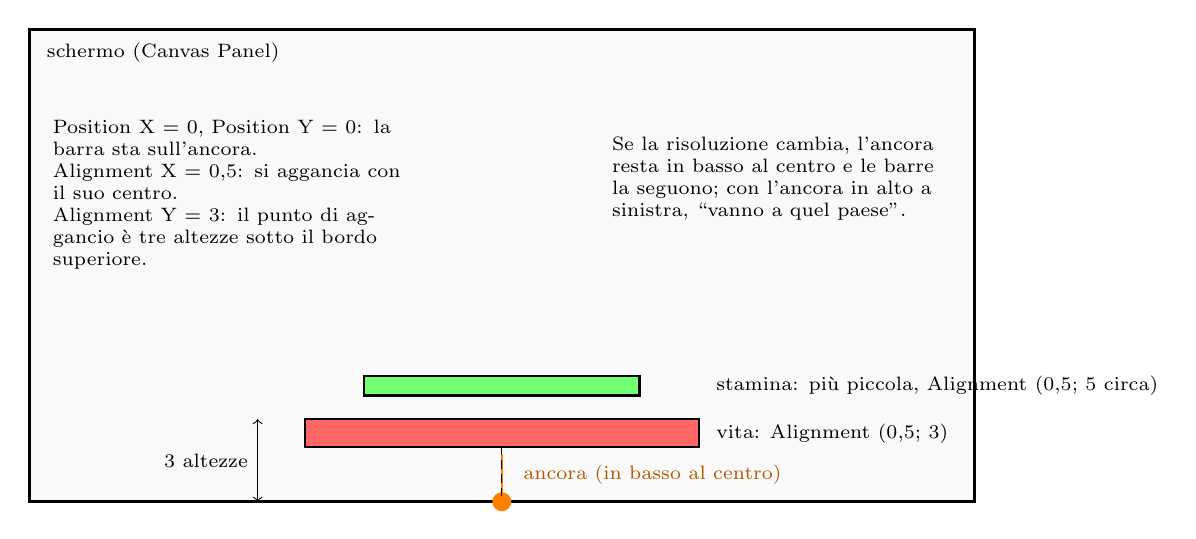
\begin{tikzpicture}[font=\footnotesize, x=1cm, y=1cm]
  % schermo
  \draw[very thick, fill=gray!5] (0,0) rectangle (12,6.0);
  \node[anchor=north west, font=\scriptsize] at (0.1,5.95) {schermo (Canvas Panel)};
  % ancora in basso al centro
  \fill[orange] (6,0) circle (0.12);
  \draw[orange, thick] (6,0) -- (6,0.6);
  \node[orange!70!black, font=\scriptsize, anchor=west] at (6.15,0.35) {ancora (in basso
    al centro)};
  % barra vita: alignment 0.5, 3 -> altezza 0.35 -> bordo superiore a 3*0.35=1.05
  \draw[thick, fill=red!60] (3.5,0.70) rectangle (8.5,1.05);
  \node[font=\scriptsize, anchor=west] at (8.6,0.87) {vita: Alignment (0,5; 3)};
  % barra stamina: posizione indicativa
  \draw[thick, fill=green!55] (4.25,1.35) rectangle (7.75,1.6);
  \node[font=\scriptsize, anchor=west] at (8.6,1.48) {stamina: più piccola, Alignment
    (0,5; 5 circa)};
  % pivot
  \draw[densely dashed] (6,0.70) -- (6,0);
  \draw[<->, thin] (2.9,0) -- node[left, font=\scriptsize]{3 altezze} (2.9,1.05);
  \node[font=\scriptsize, text width=4.6cm, align=left] at (2.6,3.9) {Position X = 0, Position
    Y = 0: la barra sta sull'ancora.\\ Alignment X = 0,5: si aggancia con il suo centro.\\
    Alignment Y = 3: il punto di aggancio è tre altezze sotto il bordo superiore.};
  \node[font=\scriptsize, text width=4.4cm, align=left] at (9.6,4.1) {Se la risoluzione
    cambia, l'ancora resta in basso al centro e le barre la seguono; con l'ancora in alto
    a sinistra, ``vanno a quel paese''.};
\end{tikzpicture}
\caption{Ancore, posizione e allineamento di un widget nel Canvas Panel. La posizione si
misura dall'ancora, l'allineamento sposta il punto dell'elemento che si aggancia
all'ancora, in frazioni della sua dimensione. Schema ricostruito; proporzioni indicative.}
\label{ue11:fig:ancore}
\end{figure}

\paragraph{Approfondimento: ancore e Percent nel libro.} Romero e Sewell (capitolo 7):
``poiché le dimensioni e i rapporti degli schermi possono variare, vogliamo assicurarci
che gli elementi della UI restino nella stessa posizione relativa sullo schermo. Le ancore
servono a definire la posizione desiderata di un widget sul canvas, indipendentemente
dalla dimensione dello schermo.'' Il simbolo a forma di fiore che si vede nel Designer si
chiama \emph{Anchor Medallion}, ``e rappresenta la posizione dell'ancora dell'elemento
selezionato''; la seconda edizione aggiunge che si può anche trascinare direttamente il
fiore nel punto voluto, o espandere \emph{Anchors} per i controlli di precisione. Uno dei
quesiti di fine capitolo chiede se ``i valori X e Y della posizione di un elemento in un
canvas sono sempre relativi all'angolo in alto a sinistra dello schermo'': la risposta è
no, sono relativi all'ancora, che è esattamente ciò che Guido ha scoperto. Sul Percent:
``l'intervallo dei valori va da 0,0 (vuota) a 1,0 (piena)''. Il libro anticipa anche il
motivo per cui serve una divisione: le sue variabili di vita e stamina hanno valore di
default 1,0 proprio perché ``questo valore è usato dai UI meters, che mostrano il grado di
riempimento fra 0,0 e 1,0''. La lezione invece tiene la vita in punti (10) e la stamina in
centesimi (100), e converte al momento di disegnare.

% ---------------------------------------------------------------------
\section{L'HUD sullo schermo: Initialize, Create Widget e Add to Viewport}
\label{ue11:sec:viewport}

\paragraph{L'evento d'inizializzazione.} Nel \textbf{Graph} del widget (``in alto a
destra, Designer e Graph: se clicchi su Graph vai direttamente là''), si tolgono gli eventi
predefiniti e si crea un \textbf{Custom Event}: \textbf{InitializeHealthBar}. Gli serve un
input, ``la referenza stessa al player'': nei Details dell'evento, sotto \emph{Inputs}, il
più, nome \textbf{PlayerRef}, tipo la classe del proprio personaggio (``io ho BP\_Bot2,
ma deve essere il nome del vostro character''), \textbf{Object Reference}: ``quella
azzurra, deve essere azzurra''. A che serve? ``Chiamerà l'Event Dispatcher'': il personaggio
dirà ``ehi, fammi esistere questa UI, mettimela sullo schermo'', e a quel punto bisogna
``bindare l'evento al fatto di inizializzare la barra, quindi dargli subito il valore di
quant'è la vita''. (A chi chiede ``com'è che sotto c'è la freccia bianca?'': è l'evento con
il suo input, che si aggiunge dai Details.)

\paragraph{Il Begin Play del personaggio.} ``Innanzitutto, buona regola, dobbiamo passargli
la PlayerRef.'' In BP\_Bot2, all'\textbf{Event BeginPlay}: ``quando il gioco inizia,
vogliamo che l'HUD, quindi questa schermata, la sua Progress Bar e tutto quanto, vada a
esistere nel mondo, nella nostra viewport''.
\begin{enumerate}
  \item \textbf{Create Widget} (``scusate, non \emph{Add}: è Create Widget''). Il pin
        \textbf{Class} chiede ``la tipologia di asset che andiamo a creare'': WB\_HUD;
  \item il \textbf{Return Value} si promuove a variabile, \textbf{AsHUD}: ``non lo useremo,
        però è una buona cosa sempre fare una referenza, perché magari volete comunicare
        altre volte con il nostro HUD e cambiargli dei valori'';
  \item ``questo lo crea, ma non lo mette nella viewport'': serve \textbf{Add to Viewport},
        con l'HUD come target. In Play, ``ecco a voi che la nostra barra rossa è apparsa
        a schermo'';
  \item infine, dalla variabile AsHUD, la chiamata a \textbf{InitializeHealthBar}, con
        \textbf{PlayerRef} collegato a un \textbf{Get a Reference to Self} (``fate
        \emph{self}, vi appare Get a Reference to Self''). ``Abbiamo detto: ehi, aggiungi
        questo widget alla viewport e inizializza.''
\end{enumerate}
(Durante questa parte il docente ha qualche problema di connessione: ``scusa, ho visto
adesso la chat; sto avendo problemi, devo fare un po' di manutenzione''.)

% ---------------------------------------------------------------------
\section{Il collegamento: Bind Event e Set Percent}
\label{ue11:sec:bind}

\paragraph{Il Bind.} ``Ci manca ovviamente la funzione collegata'': bisogna fare in modo
che l'inizializzazione \emph{agganci} l'aggiornamento della barra all'aggiornamento della
vita. Nel Graph del widget, dopo InitializeHealthBar, dal pin PlayerRef: \textbf{Bind
Event to E\_UpdateHealth} (la trascrizione sente ``bind e update''). Compilando dà errore,
``giustamente'': ``mi serve un evento: che evento devo collegare al fatto che io aggiorno la
mia variabile Health?''. L'evento si crea così: dal pin rosso \textbf{Event} del Bind si
trascina un filo e si sceglie \textbf{Add Custom Event}. ``Mi raccomando: non fate un
Custom Event esterno, tirate fuori proprio da Event e fate Custom Event, perché vi tira
fuori e si porta dietro i due valori che gli abbiamo dato di input, cioè CurrentHealth e
MaxHealth.'' Il nome: \textbf{UpdateHealthBar}.

\paragraph{Che cosa succede.} Una studentessa riassume: ``quindi quando viene
inizializzato, in automatico fa anche Update Health?''. ``Esatto.'' Quando il gioco
inizia, l'HUD ``binda l'evento di aggiornare la barra al nostro Update Health, cioè al
valore numerico che si aggiorna''. ``Creiamo il collegamento'': da quel momento, ``quando si
aggiorna effettivamente il nostro numero, la nostra variabile, allora avviene anche
l'update della barra''.

\paragraph{L'evento senza posti.} ``A me il Bind Event non me l'ha dato'': la studentessa
aveva creato prima, per sbaglio, un Custom Event separato e l'aveva collegato al Bind;
cancellato quello, il Bind risultava ``ancora delegato''. ``Elimina quello che hai
adesso; tira fuori da Event, Custom Event.'' La spiegazione: un Custom Event creato a mano
``non ti dà quei valori di input, CurrentHealth e MaxHealth''; ``questo qua deve essere
creato tramite il collegamento, perché noi gli abbiamo messo degli input''. ``Non deve
essere vuoto: si deve portare dietro i posti per la CurrentHealth e la MaxHealth.
Ricordiamoci il camion.''

\paragraph{Rinominare la barra.} ``Per ordine'': nel Designer, nella \textbf{Hierarchy}
(``ci permette di avere tutte le nostre cosine che abbiamo messo nella UI, tutte belle
elencate''), si seleziona la Progress Bar e con \textbf{F2} la si rinomina
\textbf{ProgressBar\_Health}.

\paragraph{Set Percent.} Nel Graph, la variabile ProgressBar\_Health si trascina
nell'evento UpdateHealthBar e da lei si tira fuori \textbf{Set Percent}. ``In questo caso
però si tratta di una percentuale, quindi è un valore da 0 a 1'': il valore è
\textbf{CurrentHealth diviso MaxHealth}, i due pin dell'evento in un \textbf{Divide}. In
Play, ``la mia barra diminuisce sempre di più, e boom, eccoci qua''
(figure~\ref{ue11:fig:hudgraph} e~\ref{ue11:fig:catena}).

\begin{figure}[htbp]
\centering
\begin{tikzpicture}[font=\scriptsize,
  ue11node/.style={draw, thick, rounded corners=4pt, align=center, fill=gray!8,
                  minimum height=0.9cm, text width=2.0cm},
  ue11ev/.style={ue11node, fill=red!12},
  ue11var/.style={ue11node, fill=blue!10, rounded corners=8pt},
  ue11exec/.style={-{Stealth[length=2.5mm]}, very thick, black!80},
  ue11data/.style={-{Stealth[length=2mm]}, thick, blue!60!black}]
  \node[font=\scriptsize\bfseries, anchor=west] at (-1.0,1.0) {BP\_Bot2, Event Graph};
  \node[ue11ev, text width=1.5cm] (bp) at (0,0) {\textbf{Event BeginPlay}};
  \node[ue11node, text width=1.7cm] (cw) at (2.4,0) {\textbf{Create Widget}\\Class:
    WB\_HUD};
  \node[ue11var, text width=1.4cm] (sh) at (4.7,0) {\textbf{Set}\\AsHUD};
  \node[ue11node, text width=1.6cm] (av) at (6.9,0) {\textbf{Add to Viewport}};
  \node[ue11node, fill=yellow!20, text width=2.5cm] (ih) at (9.7,0)
    {\textbf{Initialize\-Health\-Bar}\\PlayerRef: Self};
  \node[ue11node, fill=yellow!20, text width=2.5cm] (is) at (13.0,0)
    {\textbf{Initialize\-Stamina\-Bar}\\PlayerRef: Self (più tardi)};
  \draw[ue11exec] (bp) -- (cw); \draw[ue11exec] (cw) -- (sh);
  \draw[ue11exec] (sh) -- (av); \draw[ue11exec] (av) -- (ih);
  \draw[ue11exec, dashed] (ih) -- (is);
  \node[font=\scriptsize\bfseries, anchor=west] at (-1.0,-1.6) {WB\_HUD, Graph};
  \node[ue11ev, text width=2.5cm] (ini) at (0.3,-2.7) {\textbf{Initialize\-Health\-Bar}\\
    Custom Event, input PlayerRef};
  \node[ue11node, text width=2.5cm] (bind) at (3.9,-2.7) {\textbf{Bind Event to
    E\_UpdateHealth}\\Target: PlayerRef};
  \node[ue11ev, text width=2.5cm] (upd) at (8.3,-2.7) {\textbf{Update\-Health\-Bar}\\
    CurrentHealth, MaxHealth};
  \node[ue11node, text width=1.6cm] (div) at (10.9,-4.4) {\textbf{Divide}\\Current /
    Max};
  \node[ue11node, text width=2.6cm] (sp) at (12.4,-2.7) {\textbf{Set Percent}\\Target:
    ProgressBar\_Health};
  \draw[ue11exec] (ini) -- (bind);
  \draw[ue11data, red!60!black] (bind) -- node[below]{Event} (upd);
  \draw[ue11exec] (upd) -- (sp);
  \draw[ue11data] (upd.south) |- (div.west);
  \draw[ue11data] (div.north) -- node[right]{In Percent} (sp.south -| div.north);
\end{tikzpicture}
\caption{I due lati dell'HUD. In alto, il personaggio crea il widget, se lo salva, lo
aggiunge alla viewport e gli passa una referenza a se stesso. In basso, il widget usa
quella referenza per legare il proprio evento UpdateHealthBar all'Event Dispatcher del
personaggio: da lì in poi, ogni Call E\_UpdateHealth esegue Set Percent. La chiamata
tratteggiata si aggiunge con la stamina. Schema ricostruito.}
\label{ue11:fig:hudgraph}
\end{figure}

\begin{figure}[htbp]
\centering
\begin{tikzpicture}[font=\footnotesize,
  ue11node/.style={draw, thick, rounded corners=4pt, align=center, fill=gray!8,
                  minimum height=1.0cm, text width=2.5cm},
  ue11exec/.style={-{Stealth[length=2.5mm]}, very thick, black!80}]
  \node[ue11node, fill=orange!15] (pr) at (0,0) {\textbf{BP\_Projectile}\\{\scriptsize
    Sphere Trace, Break Hit Result}};
  \node[ue11node, fill=orange!15] (ad) at (3.4,0) {\textbf{Apply Damage}\\{\scriptsize
    Hit Actor, Base Damage 1}};
  \node[ue11node, fill=red!12] (any) at (6.8,0) {\textbf{Event Any\-Damage}\\{\scriptsize
    in BP\_Bot2}};
  \node[ue11node, fill=blue!10] (hp) at (10.2,0) {\textbf{CurrentHealth}\\{\scriptsize
    Subtract, Clamp, Set}};
  \node[ue11node, fill=yellow!20] (call) at (10.2,-2.2) {\textbf{Call
    E\_UpdateHealth}};
  \node[ue11node, fill=green!10] (ev) at (6.8,-2.2) {\textbf{Update\-Health\-Bar}\\
    {\scriptsize in WB\_HUD (legato)}};
  \node[ue11node, fill=green!10] (pb) at (3.4,-2.2) {\textbf{Set Percent}\\{\scriptsize
    Current / Max}};
  \node[ue11node, fill=green!20] (bar) at (0,-2.2) {\textbf{barra rossa}\\{\scriptsize
    sullo schermo}};
  \draw[ue11exec] (pr) -- (ad); \draw[ue11exec] (ad) -- (any);
  \draw[ue11exec] (any) -- (hp); \draw[ue11exec] (hp) -- (call);
  \draw[ue11exec] (call) -- (ev); \draw[ue11exec] (ev) -- (pb);
  \draw[ue11exec] (pb) -- (bar);
  \node[font=\scriptsize, text width=13cm, align=center] at (5.1,-3.6) {Il proiettile non
    sa nulla della UI, e la UI non sa nulla del proiettile: ognuno parla solo con il
    personaggio.};
\end{tikzpicture}
\caption{Il percorso completo di un colpo, dal proiettile alla barra. Il sistema di danno
di Unreal collega il proiettile al personaggio; l'Event Dispatcher collega il personaggio
all'HUD. Schema riassuntivo.}
\label{ue11:fig:catena}
\end{figure}

\paragraph{I problemi dei presenti.} ``Ci siete, ragazzi?'' Tre casi.
\begin{itemize}
  \item \textbf{Set Percent introvabile.} ``Non mi dà il Set Percent'', e nemmeno i
        Details per cercarlo. Primo controllo: nel Designer, la Progress Bar deve avere la
        spunta \textbf{Is Variable}, altrimenti nel Graph non esiste come variabile. I
        Details mancanti si riaprono da \textbf{Window}, \textbf{Details}. La spunta c'era;
        il vero errore è un altro: lo studente cercava Set Percent trascinando da un altro
        nodo. ``Ah, ok, lo facevo da qua'': Set Percent si trova solo \emph{tirando fuori
        dalla variabile} ProgressBar\_Health, che va presa dalla sezione \emph{Variables}
        (``se non ce l'hai, c'è la tendina'') e trascinata nel grafo. Per la divisione:
        ``tiri fuori dalla CurrentHealth e fai lo slash'', oppure si scrive
        \emph{divide}; poi ``questo diviso per quell'altro''.
  \item \textbf{La torretta che non spara}, a un'altra studentessa: rimandata alla pausa.
  \item \textbf{La barra che non scende.} ``La vita la perdo, perché poi respawno; tuttavia
        graficamente non scende la barra.'' Il Bind c'è, il danno è 1 (``l'ho messo come
        variabile''), la vita è 10. Un Print String dopo il Set Percent, ``attaccalo a In
        String'' (``collega quello verde a quello rosa''), non stampa niente. Allora
        \textbf{F9} sull'evento UpdateHealthBar: ``dice: sta facendo questo evento?''. Il
        breakpoint non scatta. In BP\_Bot2 si scopre perché: nel Begin Play mancava la
        chiamata a \textbf{InitializeHealthBar} dopo Add to Viewport. ``Non stai dicendo al
        gioco che, quando inizia, se io ho dato la vita, mi aggiorni pure la barra.'' Si
        aggiunge da AsHUD, con Self nel PlayerRef; si toglie il breakpoint (``se no te lo
        farà ogni volta''). ``Perfetto, grazie.''
\end{itemize}

\paragraph{Il portatile surriscaldato.} Un altro studente non riesce a seguire: ``sta
andando a scatti'', ``è troppo surriscaldato il computer''. Il consiglio, per tutti: ``per
chi ha un portatile, prendetevi quelle basette con le ventole'': ``col portatile quello
diventa un vulcano a un certo punto''. Lo studente ce l'ha già: ``ah, ok. Quindi sta proprio
andando pesantissimo''. ``Lascialo riposare il nostro soldato, tranquillo: tanto poi c'è la
registrazione.''

\paragraph{Approfondimento: Bind Event contro i Binding del libro.} Qui la lezione e il
libro scelgono due strade diverse, e vale la pena capire perché. Romero e Sewell
(capitolo 7) usano i \textbf{Binding} delle proprietà: accanto al campo \emph{Percent}
della Progress Bar c'è un pulsante \emph{Bind}; scegliendo \emph{Create Binding}, l'editor
crea una funzione che restituisce il valore, in cui gli autori mettono \emph{Get Player
Character}, \emph{Cast To FirstPersonCharacter} e il Get della vita. ``I Binding ci danno
la possibilità di legare variabili o funzioni di un Blueprint a un Widget. Ogni volta che
la variabile o la funzione è aggiornata, il cambiamento si riflette automaticamente nel
Widget.'' Il prezzo, per il funzionamento generale di UMG, è che una funzione di Binding
viene valutata \emph{a ogni frame}, che il valore sia cambiato o no (e, nell'esempio del
libro, con un cast a ogni valutazione). Lo schema della lezione è \emph{a eventi}: la barra
si aggiorna solo quando il personaggio chiama E\_UpdateHealth, cioè quando la vita cambia
davvero. Per due barre la differenza di prestazioni è trascurabile; diventa importante
negli HUD con molti elementi, e soprattutto rende esplicito \emph{chi} aggiorna \emph{che
cosa}. Sul Bind Event, invece, il libro (capitolo 4) dice la stessa cosa del docente:
``c'è un nodo Bind Event che lega un evento a un altro evento o a un Event Dispatcher, che
può stare in un altro Blueprint. Quando un evento è chiamato, tutti gli altri eventi legati
a lui sono chiamati'', e il Custom Event si crea trascinando ``dal pin rosso del nodo Bind
Event'' e scegliendo \emph{Add Custom Event}. Un dettaglio generale: un Custom Event creato
dal pin riceve automaticamente la \emph{firma} del dispatcher (i suoi input); se in seguito
si aggiungono input al dispatcher, gli eventi legati vanno aggiornati, e l'editor lo segnala
con un errore di firma alla compilazione.

% ---------------------------------------------------------------------
\section{La seconda barra e la corsa}
\label{ue11:sec:corsa}

``Abbiamo un quarto d'oretta. Sai che facciamo? Andiamo a creare la nostra barra della
stamina e facciamo insieme la stamina, così dopo magari facciamo qualcos'altro, che è il
menu in questo caso.''

\paragraph{La barra copiata.} ``Più che metterne una nuova'', nel Designer di WB\_HUD si
copia la barra della vita con \textbf{Ctrl+C} e \textbf{Ctrl+V}. La copia ha ancora
l'ancora in basso al centro; si azzerano le posizioni, \textbf{Alignment} X a \textbf{0,5}
e Y più alto, perché stia sopra la barra rossa (il docente dice ``non 3, ma la mettiamo
tipo a 2, e facciamo 5'', poi ``facciamo 5''), la si fa ``un pochino più piccola'' (con i
campi della dimensione, ``1,8, ma sì, 2'': ``questi rettangolini servono per essere un po'
più precisi''), e verde. ``Se volete, ragazzi, sbizzarritevi: i colori, proprio pastelli in
mano, fate come volete.''

\paragraph{InitializeStaminaBar.} ``Facciamo la stessa identica cosa per l'inizializzazione
della barra'': nel Graph, un altro Custom Event, \textbf{InitializeStaminaBar}, con lo
stesso input \textbf{PlayerRef} (``fortunatamente, se avete già fatto l'input, vi dice già:
ce l'ho, PlayerRef''). ``Per adesso lo lasciamo così, perché dobbiamo creare un altro
Event Dispatcher, che sarà invece l'update della stamina.''

\paragraph{IA\_Run.} Torniamo nel bot: ``dobbiamo far correre il nostro player''. Serve
un'\textbf{Input Action} nuova, \textbf{IA\_Run}, accanto a IA\_Look, IA\_Move e IA\_Jump;
la si era fatta la volta scorsa per il cavaliere, e ``fortunatamente'' basta una volta:
``questa è la bellezza del context: la mappatura degli input è separata dal player'', e
``la posso passare da player a player''. Per chi non ce l'ha:
\begin{enumerate}
  \item da un'azione qualsiasi, tasto destro, \textbf{Show in Folder View}; si
        \textbf{duplica} IA\_Jump e la si chiama IA\_Run. ``Se non sbaglio, Jump e Run
        sono uguali'': entrambe hanno un valore booleano (\emph{Digital});
  \item nell'\textbf{IMC} (\emph{Input Mapping Context}), il più, IA\_Run, e nella
        tendina la \textbf{tastiera}: ``cliccate sulla tastiera, premete Shift'', ``in modo
        da dire: guarda che questo è l'input collegato alla corsa''.
\end{enumerate}
``Io l'ho spiegato molto velocemente, perché so che, se qualcuno nel caso non avesse
visto, poi mi dica.''

\paragraph{Gli stati dell'evento.} Nel bot, l'evento \textbf{IA\_Run} mostra le sue uscite
(\emph{Triggered}, \emph{Started}, \emph{Ongoing}, \emph{Canceled}, \emph{Completed});
``in questo caso ci interesseranno solamente lo \textbf{Started} e il
\textbf{Completed}'': l'inizio e la fine della pressione.

\paragraph{Camminare di default.} ``Per dire già che il player deve camminare di default'',
si guarda il Blend Space del bot: la camminata è a 250, ``facciamo 300, un po' più alto''.
Nel \textbf{Character Movement}, categoria \emph{Character Movement: Walking},
\textbf{Max Walk Speed} a \textbf{300}: ``da adesso in poi il nostro character camminerà''.
(Se i passi non suonano, ``lo fixiamo poi'': il docente aveva aggiunto i suoni dei passi
anche all'animazione di camminata prima della lezione, ``perché prima solamente
correvamo''.)

\paragraph{Correre.} Due \textbf{Set Max Walk Speed}, entrambi con il Character Movement
come target (``ricordatevi di tutti e due di collegarli''): uno allo \textbf{Started}, a
\textbf{500}, uno al \textbf{Completed}, a \textbf{300}. (Il docente dice prima 600, poi
``500 era? Facciamo 500, va bene'', il valore massimo del Blend Space.) In Play: ``cammino;
Shift, corro; Shift, lascio''. ``Sicuramente possiamo mettere un po' di smooth
all'animazione'', con un \emph{blend in} e un \emph{blend out}: ``questo è un fix che
possiamo fare dopo, tranquillamente''.

\paragraph{La stamina di Dark Souls.} ``Qualcuno di voi ha in mente Dark Souls? La stamina
di Dark Souls, o in generale, molto spesso la stamina funziona in questo modo'': ``viene
persa durante un quantitativo di tempo, se si fa una certa azione, in questo caso correre:
viene levata gradualmente'', e quando l'azione smette ritorna su piano piano. ``Visto che
parliamo di tempo, useremo due \textbf{timer}'', come per la torretta, ``per far sì che
queste due cose vadano a scalare nel tempo''. Mancano cinque minuti alla pausa: ``facciamo
adesso un piccolo timer, oppure vogliamo andare già in pausa?''. Si va in pausa: ``la
prova è 25'', ``facciamo 17 e 55 e ci rivediamo''.

\paragraph{Approfondimento: lo sprint nel libro.} Romero e Sewell costruiscono lo sprint nel
capitolo 6 con il sistema di input precedente (l'\emph{Action Mapping} ``Sprint'' sul
tasto Shift sinistro, gli eventi \emph{Pressed} e \emph{Released}) e due \emph{Set Max
Walk Speed}, esattamente come la lezione con l'Enhanced Input (Started e Completed). Nel
capitolo 8 fanno un'osservazione di design che spiega perché la stamina serve: senza un
vincolo, ``non ci sarebbe niente a scoraggiare il giocatore dal tenere sempre premuto
Shift mentre si muove''; ``se un'opzione è così attraente che il giocatore si sente
costretto a usarla sempre, allora non aumenta il numero di scelte interessanti''. ``Dal
punto di vista del giocatore, il risultato sarebbe lo stesso se aumentassimo semplicemente
la velocità di base fino a quella dello sprint.'' La stamina trasforma lo sprint in una
\emph{risorsa}: correre ora significa non poter correre fra poco. È la stessa logica della
stamina di Dark Souls, dove la stessa barra è condivisa da corsa, schivata, parata e
attacco, e ogni scelta ha un costo.

% ---------------------------------------------------------------------
\section{La pausa: le torrette e i bot degli studenti}
\label{ue11:sec:pausa}

La pausa, come spesso in questo corso, diventa uno sportello di correzioni. Il docente
resta collegato e guarda i progetti uno alla volta, in condivisione di schermo
(``quando condividi, fai \emph{condividi schermo}, non condividere Unreal, perché è più
facile: stiamo schermando più grande'').

\paragraph{Lo Shift che non corre.} Il primo studente: ``se mi muovo normalmente cammina,
se premo Shift non corre''. ``Allora c'hai qualche cosa che non va nell'IA\_Run.'' La cosa
resta in sospeso: il problema dello stesso tipo tornerà, più grave, alla fine della lezione
(sezione~\ref{ue11:sec:barrastamina}).

\subsection{La torretta di Tommaso}

``Io entro, mi vede, ma non spara.'' Il tag Player c'è.
\begin{enumerate}
  \item \textbf{La collisione della mesh del bot}: ``non l'avevo messa''. Mesh, Collision,
        Custom, Detection Turret in Block (e Projectile Trace: ``va benissimo''). Ora la
        torretta lo segue, ma non spara.
  \item \textbf{Il Trace Channel}: nella torretta, il trace di rilevamento usava il canale
        sbagliato. ``Cambia Trace Channel'' a \textbf{Detection Turret} (``no, no, torna
        indietro; Ctrl+Z''). ``Ok, benissimo.''
  \item \textbf{La funzione dello spawn}: alla torretta di Tommaso manca proprio la
        funzione che fa nascere il proiettile. Il docente gliela passa con ``un
        trucchettino'': ``la cosa bella dei Blueprint è che puoi incollarli in un file di
        testo, copiarli tutti quanti''. Seleziona i nodi della sua funzione, Ctrl+C, li
        incolla in un file \emph{.txt} (``Fix, funzione Spawn'') e glielo manda su
        Discord, in privato. Tommaso scarica il file, ne copia tutto il testo e lo incolla
        con Ctrl+V nel grafo di Unreal: i nodi ricompaiono.
  \item \textbf{Sistemare l'incollato}: ``adesso c'hai degli errori, eh? Perché devi
        sistemarlo''; ``prima fix, poi ordina''. La funzione si rinomina con F2
        \textbf{Spawn Projectile}. Servono i due punti di uscita: nei Components, Add,
        due \textbf{Scene Component}, \textbf{ProjectileSpawn1} e \textbf{ProjectileSpawn2}
        (copiati con Ctrl+C e Ctrl+V), agganciati al \textbf{cannone} della torretta e
        spostati ``ai bocchettoni della mesh'', ``poco fuori la canna''.
  \item \textbf{Lo Spawn Actor rifatto}: il nodo incollato dà un errore sull'\emph{Spawn
        Actor} (``non ti spawno nessun actor''); l'errore sull'\emph{Instigator} invece
        ``va bene, non ci interessa''. ``Facciamo prima'': si cancella e si rifà
        \textbf{Spawn Actor from Class}; tasto destro sullo \emph{Spawn Transform},
        \textbf{Split Struct Pin}; si collegano Location e Rotation dei due Scene; la
        \textbf{Class} è il proiettile, BP\_Projectile.
  \item Una curiosità di Tommaso, nel frattempo: ``pure la barra della stamina, io gli ho
        dato un colore, ma me la dà grigia''. ``Forse è vuota'': il \emph{Percent} è a 0,
        e una Progress Bar vuota mostra solo lo sfondo. ``Faccio 1.''
  \item \textbf{Chiamare la funzione}: la torretta ancora non spara, ``perché non
        spawni'': nello \emph{Shoot}, al posto delle due vecchie chiamate, va chiamata la
        nuova \textbf{Spawn Projectile}.
  \item \textbf{Le collisioni della torretta}: il proiettile non deve fermarsi sulla
        torretta stessa. Sul cannone, sulla sfera di rilevamento e sul pivot, il canale
        Projectile Trace va su \textbf{Ignore} (``devi ignorare tutto, anche il pivot'').
\end{enumerate}
La torretta di Tommaso ancora non spara; ``aspetta, adesso facciamo fare Lucrezia, che è
un po' che aspetta''. Si riprenderà dopo la pausa.

\subsection{Il bot di Lucrezia, risolto}

\paragraph{Il Validated Get sulla variabile sbagliata.} Con Shift il bot di Lucrezia ora
``va più veloce'': ``quello almeno va benissimo''; quindi il personaggio si muove, ``è un
problema di animazioni''. Il docente esclude un doppio scheletro (``non vorrei che avessi
un doppio scheletro e te l'avessi fatto su un altro'': ne ha uno solo), poi mette un
Print String sull'uscita \textbf{Is Not Valid} del Validated Get, all'inizio dell'Update.
Stampa: ``ecco il nostro problema: la referenza a questo actor non è valida''. Il motivo:
``hai messo nel Validated Get la variabile del PB\_Bot, non del BP\_Bot, che sono due
diverse'': nell'Animation Blueprint c'erano due variabili quasi omonime, e il Validated
Get controllava quella che l'Initialize non riempiva mai. Si cancella, si prende la
variabile giusta (\textbf{AsBP\_Bot}), tasto destro, \textbf{Convert to Validated Get}, si
ricollega. ``Dovremmo aver scoperto l'arcano.'' ``Era lui.''

\paragraph{La regola di ritorno all'Idle.} Ora il bot anima, ma ``continua a camminare sul
posto'' quando si ferma. Nella State Machine, la regola Walk $\rightarrow$ Idle era
\emph{GroundSpeed $<$ 0}: ``attenzione, non è minore, è \textbf{minore o uguale}'',
perché una velocità negativa non esiste (la lunghezza di un vettore è sempre $\ge 0$), e con
il minore stretto la regola non è mai vera (``solo se sarà meno uno la velocità'').

\paragraph{Il Lean, di nuovo.} Correndo e girando, il bot ``non si inclina tantissimo'':
la stessa correzione fatta a inizio lezione (``come abbiamo fatto anche con Tommaso'': la
trascrizione attribuisce qui a Tommaso il Lean corretto all'inizio). Nel Blend Space i
campioni da $\pm 10$ a $\pm 1$, poi l'asse, nelle \emph{Axis Settings} dei Details, da $-1$
a 1. ``Ecco che si piega leggermente.''

\paragraph{La torretta di Lucrezia.} Poi la torretta, aperta con \emph{Edit BP\_Turret} dal
livello (``lo fai diretto''). ``Questo è un po' incasinato, eh? Vabbè, tranquillo.'' In
ordine:
\begin{itemize}
  \item \textbf{Begin Overlap}: il fix di inizio lezione, Get Player Pawn al posto
        dell'Other Actor nel Set di PlayerTarget;
  \item \textbf{Move Turret} (la rotazione verso il bersaglio): il nodo di rotazione
        usato era un altro, e si sostituisce con \textbf{Find Relative Look at
        Rotation}, che vuole uno \emph{Start Transform} (``non ti serve il Get Actor
        Rotation, ma devi invocare il \textbf{Get Actor Transform}'', ``pinnetto
        arancione per pinnetto arancione'') e una \emph{Target Location}, il \textbf{Get
        Actor Location} del PlayerTarget. Del risultato, con \emph{Split Struct Pin}, si
        usa la \textbf{Z} (lo Yaw) come \emph{Target} dell'interpolazione; un vecchio
        ``meno'' non serve più; nel \emph{Delta Time} va \textbf{Get World Delta Seconds}.
        La trascrizione, qui, è troppo frammentaria per ricostruire il grafo nodo per nodo;
        il senso è quello della rotazione della torretta costruita nelle lezioni
        precedenti;
  \item \textbf{Shoot}: Branch, Sequence, i due \emph{Do Once} con lo Spawn Projectile e il
        Delay, il \emph{Fire Rate}: ``va benissimo'';
  \item un secondo \emph{On Component Begin Overlap} rimasto da una prova (``probabilmente
        una cosa che avevo cancellato'', ``l'avevo spostata''): si elimina; l'\emph{End
        Overlap} e il Tick si tengono;
  \item \textbf{il tag}: la torretta ancora non la segue. Il tag Player era stato messo nei
        \emph{Component Tags} della mesh: ``attenzione, non della mesh, ma quello sotto'':
        i \textbf{Tags} dell'\emph{actor}, e con la stessa maiuscola.
\end{itemize}

\paragraph{Il proiettile assassino.} Ora la torretta spara (``sei un po' alta''), ma
emergono tre problemi del proiettile, uno dopo l'altro.
\begin{enumerate}
  \item I proiettili urtano la camera del personaggio: sulla \emph{Sphere} del proiettile,
        Collision, \textbf{Camera} su \textbf{Ignore}.
  \item I proiettili ``non si distruggono se il character gli va addosso'': la Sphere
        Trace aveva \textbf{Radius 0}, ``quindi è grande niente''. A \textbf{20}.
  \item Ora un colpo e il bot ``si blocca proprio tutto'', anche se la vita non è finita.
        Nel proiettile, dopo il colpo, c'era un \textbf{Destroy Actor} con l'\emph{Hit
        Actor} come target (un ramo chiamato \emph{Kill Target}): ``se colpisco qualcosa,
        distruggimi quello che ho colpito''. Il proiettile cancellava il personaggio dal
        mondo. Al suo posto: \textbf{Apply Damage} (Hit Actor nel Damaged Actor, Base
        Damage 1), e poi \textbf{Destroy Actor} senza target, cioè \emph{self}: ``quando
        collide con qualcosa, distruggi il proiettile: si autodistrugge''.
\end{enumerate}

\paragraph{La vita a zero e la NewVar.} Ora il bot ``muore praticamente subito'': la
\textbf{MaxHealth} aveva default 0, e il Clamp riduceva a zero qualunque vita. MaxHealth a
10. Poi il contrario: il primo colpo toglie vita, ``poi adesso è immortale''. Nell'Event
AnyDamage c'era un Set su una variabile \textbf{NewVar}, creata per sbaglio, invece che
sulla CurrentHealth: ``stai praticamente mettendo una variabile nuova come vita''. Si
sostituisce con \emph{Set CurrentHealth}, ricollegando il Return Value del Clamp e il
valore al Branch del minore o uguale. ``Perfetto. Grazie mille.''

\paragraph{Approfondimento: i Blueprint come testo.} Il ``trucchettino'' del file di testo
funziona perché Unreal copia i nodi negli appunti in un formato testuale (lo stesso
formato \emph{T3D} usato per copiare gli actor fra livelli): ogni nodo diventa un blocco
\texttt{Begin Object} \dots\ \texttt{End Object} con la sua classe, la posizione nel grafo,
i valori dei pin e i collegamenti. Incollando quel testo in un altro grafo, anche di un
altro progetto, l'editor ricrea i nodi. È il modo più rapido per condividere un pezzo di
logica in chat o su un forum, ed esistono siti che lo visualizzano come immagine. Il
limite è quello visto a lezione: i riferimenti a variabili, componenti e funzioni del
Blueprint d'origine non esistono nel Blueprint di destinazione, e i nodi che li usano
arrivano ``rotti'' e vanno ricollegati o ricreati (come gli Scene Component e lo Spawn
Actor di Tommaso). Questa è una nozione generale dell'editor, non trattata nei due libri.

% ---------------------------------------------------------------------
\section{Dopo la pausa: ancora la torretta, e gli annunci}
\label{ue11:sec:annunci}

``Eccoci qua, ragazzi, siamo ritornati.'' Tommaso ha provato a togliere e rimettere la
torretta: niente.

\paragraph{L'Event Tick che manca.} ``Io credo che sia \emph{not valid} il PlayerTarget,
probabilmente.'' Il Begin Overlap e il timer sono giusti; ``ah, ti manca il Tick''.
Nell'Event Graph della torretta non c'è l'\textbf{Event Tick} che, a ogni frame, controlla
il bersaglio e spara. Si ricrea: Event Tick, \textbf{Is Valid} (``punto interrogativo,
quello sotto'') con il PlayerTarget come oggetto, e sull'uscita \emph{Is Valid} la
funzione \textbf{Shoot}. La torretta spara.

\paragraph{Fire Rate e velocità.} ``È un po' lento a sparare'': il \textbf{Fire Rate}, fra
le variabili della torretta, è a 0,2 (la trascrizione dice ``02''); il docente suggerisce
un altro valore (``facciamolo 0,7''; il suo è 0,5): dalla trascrizione non si capisce se
il valore sia un intervallo fra i colpi o un'altra cosa nel grafo di Tommaso, e il capitolo
non lo ricostruisce. ``Il proiettile è molto lento'': nel proiettile, il componente
\textbf{Projectile Movement}, \textbf{Initial Speed} e \textbf{Max Speed} a \textbf{1000}.

\paragraph{Il danno che non arriva alla barra.} ``Però non prendo danno.'' Il proiettile ha
l'Apply Damage, ``va bene così''; nel BP\_Bot, però, l'\textbf{Add to Viewport} non era
collegato con il pin di esecuzione all'InitializeHealthBar (``vedi che non è stato
attaccato''). E non basta: nell'Event AnyDamage il Set era su \textbf{MaxHealth} invece che
su CurrentHealth (``ha impostato MaxHealth, non CurrentHealth''). Corretti entrambi:
``vediamo se muoio''. ``Ottimo, perfetto: di solito tutto il casino.''

\paragraph{Il calendario.} Prima di riprendere, gli annunci.
\begin{itemize}
  \item Il \textbf{menu}: ``se non ce la facciamo a fare il menu oggi, lo facciamo la
        prossima volta, e tanto la prossima volta sarà l'ultima lezione che avremo''.
  \item Dopo: ``poi avrete Davide, quindi avrete martedì con me e Davide''; ``poi
        inizierete a fare roba di \textbf{level design}''.
  \item Manca ``un piccolo asset da fare'', le \textbf{porte}: ``possiamo farlo
        tranquillamente la prossima volta, o ve lo lascio come compito, perché sono sicuro
        che lo sapete fare''. ``La timeline l'abbiamo già affrontata'' (il compito è
        descritto nella sezione~\ref{ue11:sec:chiusura}).
\end{itemize}
(``Non stai condividendo?'' ``Ah, ok. Grazie mille, Lucrezia.'')

% ---------------------------------------------------------------------
\section{I due timer della stamina}
\label{ue11:sec:timer}

``E adesso incominciamo a fare questo bellissimo scattino.'' Si torna al bot del docente
(``il proiettile non ci serve più; ci serve botolino''). Il movimento c'è già (500 e 300
sull'IA\_Run); ``abbiamo detto che dobbiamo fare due timer ben distinti: uno che la consuma
e uno che la riporta al suo massimo, piano piano nel tempo''.

\subsection{Il timer che consuma}

\paragraph{Set Timer by Event.} Dopo il Set Max Walk Speed a 500 (lo Started), un
\textbf{Set Timer by Event}.
\begin{itemize}
  \item il pin \textbf{Time} si promuove a variabile, \textbf{TimeStamina}, ``in modo tale
        da avere questa variabile molto più controllabile''; default \textbf{0,05}
        (impostato poco dopo: ``piccola cosa, semplicemente non l'abbiamo impostato''):
        ``questo è il tempo in cui verrà eseguito il timer, ogni 0,05 secondi'';
  \item \textbf{Looping} attivo; \textbf{Max Once Per Frame} attivo;
  \item ``il timer, come abbiamo visto le scorse volte, è un evento collegato'': dal pin
        rosso \textbf{Event} si crea un Custom Event, \textbf{StaminaDeduction}.
\end{itemize}

\paragraph{Le variabili.} ``Lo stesso discorso vale come per la Health'': due Float,
\textbf{CurrentStamina} e \textbf{MaxStamina}, entrambe a \textbf{100}.

\paragraph{StaminaDeduction.} Il corpo è quasi identico a quello della vita:
\begin{enumerate}
  \item CurrentStamina \textbf{Subtract} \textbf{1} (``verrà sottratto di 1 ogni 0,05
        secondi'');
  \item \textbf{Clamp (float)}, fra 0 e MaxStamina (``il nostro valore oscillerà fra un
        minimo di 0 e un massimo di MaxStamina, che è 100'');
  \item \textbf{Set CurrentStamina}: ``farà 99, 98, 97\dots''.
\end{enumerate}
``Questo è lo stesso discorso che vale per la Health, è quasi praticamente medesimo.''

\paragraph{Quando fermarsi: OR con Is Falling.} Poi un \textbf{Branch} (``tenete proprio
B'' e cliccate: la scorciatoia del Branch): se la CurrentStamina è \textbf{minore o uguale
a zero}, si fermerà la corsa (``ancora non abbiamo la funzione, ma la lasciamo così''). E
una piccola accortezza nata ``durante il testing'': ``ci sono dei problemi anche nel caso
noi stiamo cadendo''. ``Io tengo premuto il tasto mentre sto cadendo: non voglio che la
stamina venga consumata, perché non stiamo correndo effettivamente.'' Dal Character
Movement, \textbf{Is Falling} (``ce ne sono due: prendete quello \emph{Nav Movement}'',
quello con l'ingresso blu e l'uscita rossa), e i due booleani in un \textbf{OR Boolean}:
``OR è l'operatore che ci permette di dire \emph{o}: ti fermi se sei minore di zero
\emph{o} se stai cadendo'' (figura~\ref{ue11:fig:deduction}).

\paragraph{Il timer che non si ferma.} Con un Print String della CurrentStamina: ``io
cammino, cammino, comincio a sprintare: i valori scendono. Ma se anche smetto di correre,
i valori continuano a scendere, perché non stoppiamo mai il nostro timer.'' La soluzione è
tenere un \emph{riferimento} al timer: il \textbf{Return Value} di Set Timer by Event (un
\emph{Timer Handle}) si promuove a variabile, \textbf{TimerDeductionStamina}, ``in modo tale
che sia più comodo controllarlo da varie parti''. Al \textbf{Completed} dell'IA\_Run, dopo
il Set Max Walk Speed a 300: un Get di TimerDeductionStamina e \textbf{Clear and Invalidate
Timer by Handle}, ``andiamo a invalidare e fermare il nostro timer''. In Play: ``corro,
smetto di correre: si è fermato a 75''.

\subsection{Il timer che ricarica}

\paragraph{Il secondo timer.} ``Altro problema: se io ricomincio a correre, ripartirà da 75,
non torna piano piano verso 100.'' Quando si smette di correre bisogna ``fare l'opposto'':
subito dopo il Clear, un altro \textbf{Set Timer by Event}, ``sempre in Looping, sempre in
Max Once Per Frame''. Per il tempo il docente usa la stessa TimeStamina, ``ma volendo si può
fare a un valore che volete voi: volete che uno si recuperi più veloce oppure più lento,
sta a voi''. Il suo evento è un Custom Event, \textbf{RegainStamina}: ``non c'è neanche
tanto da sbizzarrirci: è letteralmente la copia di questo''. Si copiano i nodi della
deduzione fino al Set e ``l'unica cosa che andiamo a cambiare è che invece di sottrarre
uno, andiamo ad aggiungere uno'': \textbf{Add} 1, Clamp, Set CurrentStamina.

\paragraph{Fermare anche lui.} Stesso schema al contrario: il Return Value si promuove a
\textbf{TimerRegainStamina}, e allo \textbf{Started} (``quando noi ricominciamo a
correre'') un \textbf{Clear and Invalidate Timer by Handle} su di lui. In Play: ``comincio a
correre, i valori cominciano a scendere; lascio, i valori piano piano risalgono fino a
100''.

\paragraph{Fermarsi a 100.} Ma arrivato a 100, il timer della ricarica continua a girare,
inutilmente. In RegainStamina, dopo il Set, un \textbf{Branch}: se la CurrentStamina è
\textbf{maggiore o uguale} alla MaxStamina, un Clear and Invalidate Timer by Handle su
TimerRegainStamina, ``cioè lo stesso timer che stiamo avendo'': ``se arrivi a 100,
smettila''. ``Non stampo più, si è fermato.''

\subsection{L'evento StopRunning}

\paragraph{La corsa che non finisce.} ``C'è una particolarità'': correndo fino a zero, ``il
nostro character non si ferma, e neanche il timer si ferma'', e il personaggio continua a
correre con la stamina vuota. Serve la funzione di \emph{smettere di correre} anche
\emph{dentro} StaminaDeduction, non solo al rilascio del tasto. ``Per comodità, invece di
fare una funzione a parte'': si stacca il \textbf{Completed} dalla sua catena (Set Max Walk
Speed 300, Clear del timer di deduzione, Set Timer della ricarica), e all'inizio della
catena si mette un nuovo Custom Event, \textbf{StopRunning}. Poi:
\begin{itemize}
  \item il \textbf{Completed} chiama StopRunning;
  \item il ramo \textbf{True} del Branch di StaminaDeduction (stamina $\le$ 0 OR Is
        Falling) chiama StopRunning.
\end{itemize}
``Questa cosa ci serve semplicemente per trasportarci il fatto di \emph{fermati}: vai a
300 di velocità e smettila di sottrarmi la stamina, da questo evento che possiamo
trasportare un po' dappertutto.'' In Play: ``corro, corro, corro, arrivo fino a zero, mi
fermo in automatico'', la stamina risale; ``e poi devo semplicemente ripremere per poter
scattare'' (lo \emph{Started} scatta solo alla pressione). ``Abbiamo fatto il nostro
sistema di stamina'' (figura~\ref{ue11:fig:timer}).

\paragraph{Ricapitolare per chi si è perso.} Una studentessa ha perso il pezzo di
RegainStamina; il docente lo ripete: copiare la catena della deduzione, sostituire il meno
con un più, il Branch con il \emph{maggiore o uguale} (``non mi trova il maggiore'': ``io
ho la tastiera più piccola, non ci ho alcuni segni''; ``allora scrivi \emph{greater
equal}''), MaxStamina e CurrentStamina nei due ingressi, sul True il Clear and Invalidate
Timer by Handle con TimerRegainStamina. Poi StopRunning: ``stacchi da qui il Completed, ci
metti un Custom Event al suo posto, e StopRunning ce lo metti anche al Completed''; la
chiamata, ``di colore azzurro'', ``tiri fuori e fai StopRunning'', anche dopo il Branch.
``Ho recuperato tutto.''

\begin{figure}[htbp]
\centering
\begin{tikzpicture}[font=\footnotesize,
  ue11node/.style={draw, thick, rounded corners=4pt, align=center, fill=gray!8,
                  minimum height=0.9cm, text width=2.1cm},
  ue11ev/.style={ue11node, fill=red!12},
  ue11var/.style={ue11node, fill=blue!10, rounded corners=8pt},
  ue11exec/.style={-{Stealth[length=2.5mm]}, very thick, black!80},
  ue11data/.style={-{Stealth[length=2mm]}, thick, blue!60!black}]
  \node[ue11ev, text width=2.3cm] (ev) at (0,0) {\textbf{Stamina\-Deduction}\\{\scriptsize
    ogni 0,05 s}};
  \node[ue11node, text width=1.9cm] (sub) at (2.6,-2.0) {\textbf{Subtract}\\{\scriptsize
    CurrentStamina $-$ 1}};
  \node[ue11node] (cl) at (5.3,-2.0) {\textbf{Clamp (float)}\\{\scriptsize 0 --
    MaxStamina}};
  \node[ue11var] (set) at (3.1,0) {\textbf{Set}\\{\scriptsize CurrentStamina}};
  \node[ue11node, fill=yellow!20, text width=2.6cm] (call) at (6.4,0) {\textbf{Call
    E\_Update\-Stamina}\\{\scriptsize (aggiunta dopo)}};
  \node[ue11node, text width=1.4cm] (br) at (9.3,0) {\textbf{Branch}};
  \node[ue11node, text width=1.5cm] (or) at (9.3,-2.0) {\textbf{OR}};
  \node[ue11node, text width=2.1cm] (le) at (7.4,-3.7) {CurrentStamina $\le$ 0};
  \node[ue11node, text width=2.8cm] (fall) at (10.8,-3.7) {\textbf{Is Falling}\\
    {\scriptsize (Nav Movement, dal Character Movement)}};
  \node[ue11ev, text width=2.0cm] (stop) at (12.2,0) {\textbf{StopRunning}};
  \draw[ue11exec] (ev) -- (set); \draw[ue11exec] (set) -- (call);
  \draw[ue11exec] (call) -- (br);
  \draw[ue11exec] (br) -- node[above, font=\scriptsize]{True} (stop);
  \draw[ue11data] (ev.south) |- (sub.west);
  \draw[ue11data] (sub) -- (cl); \draw[ue11data] (cl.north) |- ([yshift=-3mm]set.east);
  \draw[ue11data] (le.north) -- (or.south west);
  \draw[ue11data] (fall.north) -- (or.south east);
  \draw[ue11data] (or) -- node[right, font=\scriptsize]{Condition} (br);
\end{tikzpicture}
\caption{L'evento del timer che consuma la stamina. Il calcolo è lo stesso della vita, con
1 al posto del danno; la corsa si interrompe se la stamina è finita oppure se il
personaggio sta cadendo. La chiamata dell'Event Dispatcher si inserisce dopo, per la barra.
Ricostruzione dalla lezione.}
\label{ue11:fig:deduction}
\end{figure}

\begin{figure}[htbp]
\centering
\begin{tikzpicture}[font=\footnotesize,
  ue11state/.style={draw, very thick, rounded corners=10pt, align=center,
                    minimum height=1.6cm, text width=3.8cm},
  ue11tr/.style={-{Stealth[length=2.5mm]}, very thick}]
  \node[ue11state, fill=gray!10] (walk) at (0,0) {\textbf{Cammina}\\{\scriptsize Max
    Walk Speed 300}\\{\scriptsize timer RegainStamina attivo, +1 ogni 0,05 s, fino a
    100}};
  \node[ue11state, fill=green!10] (run) at (8.4,0) {\textbf{Corre}\\{\scriptsize Max
    Walk Speed 500}\\{\scriptsize timer StaminaDeduction attivo, $-1$ ogni 0,05 s}};
  \node[ue11state, fill=yellow!15, text width=3.2cm, minimum height=1.1cm] (full) at
    (0,-4.4) {\textbf{Ferma a 100}\\{\scriptsize nessun timer attivo}};
  \draw[ue11tr] ([yshift=4mm]walk.east) -- node[above, font=\scriptsize, text
    width=4.2cm, align=center]{IA\_Run \textbf{Started}: speed 500, Clear
    TimerRegainStamina, Set Timer StaminaDeduction} ([yshift=4mm]run.west);
  \draw[ue11tr] ([yshift=-4mm]run.west) -- node[below, font=\scriptsize, text
    width=4.2cm, align=center]{\textbf{StopRunning}: dal Completed, oppure stamina $\le$
    0 OR Is Falling. Speed 300, Clear TimerDeductionStamina, Set Timer RegainStamina}
    ([yshift=-4mm]walk.east);
  \draw[ue11tr] (walk.south) -- node[left, font=\scriptsize, text width=3.0cm,
    align=right]{CurrentStamina $\ge$ MaxStamina: Clear TimerRegainStamina} (full.north);
  \draw[ue11tr] (full.east) -| node[pos=0.25, below, font=\scriptsize]{IA\_Run Started}
    (run.south);
\end{tikzpicture}
\caption{I due timer della stamina come due stati. Ogni passaggio spegne il timer dello
stato che si lascia (con il suo Timer Handle) e accende quello dello stato in cui si entra.
A stamina finita la corsa si interrompe da sola; per ricominciare bisogna premere di nuovo
Shift. Schema ricostruito.}
\label{ue11:fig:timer}
\end{figure}

\paragraph{Approfondimento: la stamina nel libro.} Romero e Sewell costruiscono la stessa
meccanica nel capitolo 8, \emph{Draining and regenerating stamina}, con scelte diverse che
è utile confrontare.
\begin{itemize}
  \item \textbf{Un timer solo.} Invece di due timer, il libro usa un unico evento,
        \emph{ManageStamina}, chiamato da un timer in loop ogni \emph{Stamina Drain and
        Recharge Time} = 0,2 secondi (``questo timer chiamerà la funzione cinque volte al
        secondo''); dentro, a seconda di un booleano \emph{IsSprinting}, l'evento consuma
        o ricarica. È lo schema dei due stati della figura~\ref{ue11:fig:timer} con un solo
        orologio.
  \item \textbf{Per nome, non per handle.} Il timer è creato con \emph{Set Timer by Function
        Name} e fermato con \emph{Clear Timer by Function Name}; per non sbagliare a
        scrivere il nome, il libro lo salva in una variabile stringa
        (\emph{StaminaManagerName}), ``per evitare bug dovuti a errori di battitura''. Prima
        di crearlo controlla \emph{Does Timer Exist by Function Name}, per non avviarne
        due. La lezione usa invece il \emph{Timer Handle} restituito da Set Timer by Event,
        che identifica il timer senza nomi.
  \item \textbf{Le macro.} La logica è divisa in quattro macro (\emph{StartSprinting},
        \emph{StopSprinting}, \emph{ManageStaminaDrain}, \emph{ManageStaminaRecharge}): è
        la stessa idea dell'evento StopRunning della lezione, un nome per un pezzo di
        logica da richiamare da più punti.
  \item \textbf{Una condizione in più.} In \emph{ManageStaminaDrain} ``ci sono due
        condizioni perché il giocatore continui a correre e a consumare stamina: deve
        muoversi, e Player Stamina deve essere maggiore di zero''; il movimento si verifica
        con \emph{Get Velocity} e \emph{VectorLengthSquared} maggiore di zero (``usiamo
        VectorLengthSquared invece di VectorLength per evitare una radice quadrata''). Nella
        lezione, invece, tenere premuto Shift da fermi consuma stamina; la condizione
        \emph{Is Falling} della lezione copre un altro caso, il salto. Inoltre, alla
        pressione di Shift il libro controlla con un Branch che la stamina sia almeno pari
        al costo di un passo di corsa (\emph{Greater} OR \emph{Nearly Equal} rispetto a
        \emph{Sprint Cost}) prima di avviare lo sprint: nella lezione, a stamina vuota la
        corsa parte e viene interrotta al primo scatto del timer.
  \item \textbf{I limiti.} Il libro usa \emph{Max (float)} per non scendere sotto 0 e
        \emph{Min (float)} per non superare 1; la ricarica si ferma quando la stamina è
        \emph{Nearly Equal} a 1,0. La lezione fa entrambe le cose con il Clamp, e si
        ferma con il maggiore o uguale.
\end{itemize}
Con i numeri della lezione: un punto ogni 0,05 secondi sono 20 punti al secondo, quindi
la stamina piena (100) dura \textbf{5 secondi} di corsa e si ricarica in altri 5 secondi.
Nel libro, 0,05 di stamina (su 1,0) ogni 0,2 secondi è 0,25 al secondo, 4 secondi di
corsa; la ricarica, 0,01 ogni 0,2 secondi, impiega 20 secondi.

\paragraph{Approfondimento: Timer Handle, Clear and Invalidate, Max Once Per Frame.} Alcune
nozioni generali sui timer di Unreal, non trattate nei due libri. Il \textbf{Timer Handle}
è una piccola struttura che identifica un timer attivo nel \emph{Timer Manager} del mondo;
\textbf{Clear and Invalidate Timer by Handle} ferma quel timer e svuota l'handle, così che
un controllo successivo (\emph{Is Timer Active by Handle}, \emph{Is Valid}) dica che non
esiste più. Chiamarlo su un handle già vuoto non fa danni: per questo la lezione può
``spegnere'' il timer della ricarica allo Started anche quando non è mai partito. Se si
chiama di nuovo Set Timer by Event sullo stesso evento mentre il timer è attivo, il timer
viene reimpostato, non duplicato. Un \textbf{Time} minore o uguale a zero non avvia il timer
(lo cancella): è il motivo per cui, nella sezione seguente, il timer di una studentessa con
il Time a zero ``non partirà mai''. Infine \textbf{Max Once Per Frame}: se l'intervallo
del timer è più corto di un frame (0,05 secondi sono 20 volte al secondo; a 15 fotogrammi
al secondo un frame dura circa 0,067 secondi), senza questa opzione il timer
``recupererebbe'' le esecuzioni perse chiamando l'evento più volte nello stesso frame; con
l'opzione lo chiama al massimo una volta. La conseguenza pratica è che, a frame rate molto
bassi, la stamina della lezione scende un po' più lentamente del previsto, invece di
scendere a scatti.

% ---------------------------------------------------------------------
\section{La stamina sulla barra}
\label{ue11:sec:barrastamina}

\paragraph{E\_UpdateStamina.} ``Adesso dobbiamo collegarlo alla nostra UI.'' Un secondo
Event Dispatcher, \textbf{E\_UpdateStamina}, con due input Float, \textbf{CurrentStamina} e
\textbf{MaxStamina} (``giustamente, ragazzi, non ho dimenticato: bisogna mettere i due
input''). Va chiamato ``in tutti i momenti in cui noi aggiorniamo CurrentStamina, quindi
sia a questo timer sia all'altro'': un \textbf{Call E\_UpdateStamina} dopo il Set di
StaminaDeduction e uno dopo il Set di RegainStamina, con i valori collegati.

\paragraph{Il Begin Play.} Come per la vita: da AsHUD, dopo InitializeHealthBar, la
chiamata a \textbf{InitializeStaminaBar} con Self nel PlayerRef (figura~\ref{ue11:fig:hudgraph}).
Un problema di passaggio: uno studente aveva chiamato gli input del dispatcher in un altro
modo e poi rinominati; il nodo dava errore. ``Elimina il blocco e rimettilo'': il nodo di
chiamata si rigenera con la firma aggiornata.

\paragraph{Nel widget.} In WB\_HUD, dopo InitializeStaminaBar: dal PlayerRef, \textbf{Bind
Event to E\_UpdateStamina}; dal pin Event, Add Custom Event, \textbf{UpdateStaminaBar} (la
trascrizione, divertita, sente ``update stealth''); ``la stessa identica cosa di dividere e
fare la percentuale''. ``Ma attenzione: quale target deve essere?'' La seconda barra, che
si chiama ancora \emph{ProgressBar\_Health1} perché è una copia: la si rinomina
\textbf{ProgressBar\_Stamina}, ``per far sì che sia più esplicativa'', la si trascina nel
Graph e diventa il target del Set Percent. In Play, ``corriamo: la barra della stamina
andrà giù e ritornerà su''.

\paragraph{I problemi dei presenti.} Molti, e diversi fra loro.
\begin{itemize}
  \item \textbf{La barra subito grigia.} ``Va subito a grigio, però i valori sono quelli.''
        Nelle due Call di E\_UpdateStamina i pin non erano collegati: ``non gli passi i
        valori''. Si collegano CurrentStamina e MaxStamina, in entrambe.
  \item \textbf{Il Bind che non compare.} ``A me non dà il Bind Event per la stamina.''
        InitializeStaminaBar non aveva l'input PlayerRef: senza la referenza al personaggio
        non c'è un oggetto da cui tirare fuori il Bind. I Details mancanti si aprono da
        \textbf{Finestra}, \textbf{Dettagli} (\emph{Window}, \emph{Details}: l'editor della
        studentessa è in italiano); si aggiunge l'input, e il Bind si trova cercando
        ``stamina''.
  \item \textbf{Il timer a zero.} Nel grafo della stessa studentessa, il Set Timer by
        Event aveva il Time vuoto: ``non ti partirà mai, perché il timer è zero''. Va
        collegata la variabile TimeStamina.
  \item \textbf{L'handle mai salvato.} Il Return Value del timer della ricarica non era
        mai stato salvato: ``torna al timer'', ``prendi Set TimerRegainStamina, imposta, e
        ce l'attacchi'', con anche il pin di esecuzione, ``perché sennò quello è il
        valore, quello là, ha dietro''.
  \item \textbf{L'Initialize scollegato e la barra sbagliata.} Nel Begin Play mancava il
        collegamento dell'InitializeStaminaBar (``la Self a PlayerRef''); nel widget,
        UpdateStaminaBar va ricreato dal pin, e il Set Percent va fatto sulla barra giusta
        (che la studentessa ha chiamato \emph{ProgressBar\_Endurance}).
  \item \textbf{Il personaggio che non corre più.} Tutto collegato, ``mi toglie la barra,
        ma non mi corre il personaggio''. Il docente ripercorre la catena (Max Walk Speed a
        300 nel componente, i due Set a 500 e 300, StaminaDeduction, il minore o uguale, Is
        Falling, StopRunning) e l'IMC: lo Shift sinistro c'è. Nell'IA\_Run, nella sezione
        \emph{Triggers}, c'erano dei trigger aggiunti (un \emph{Pressed} e un
        \emph{Released}, a quanto si capisce); la trascrizione è confusa su come vengano
        sistemati, ma la corsa non riparte. Allora una prova diretta: un \textbf{Event
        Tick} con un Print String di \textbf{Get Max Walk Speed} dal Character Movement.
        ``Il problema è che ce n'hai troppi di Print String'': con \textbf{Ctrl+F}
        (\emph{Find Results}) si cercano tutti i Print String del Blueprint, con un doppio
        clic si va a ciascuno e si tolgono quelli vecchi. Il valore stampato è
        ``300, 300, 300, sempre 300, anche se tengo premuto''. Un'altra ricerca, ``Max
        Walk Speed'', scopre il colpevole: un \emph{secondo} evento IA\_Run, rimasto dalla
        lezione precedente, con i suoi Set. ``Questo lo devi levare'', ``leva tutto questo
        ambaradam''. Ora corre.
  \item \textbf{La barra che scende solo al rilascio.} Ultimo sintomo: ``a me scende quando
        mollo il tasto''. Il timer (0,05, Looping, Max Once Per Frame), StaminaDeduction e
        i suoi nodi sembrano giusti; un F9 sul primo timer non chiarisce. ``Guarda, facciamo
        una cosa: lo facciamo la prossima volta. Ricordamelo tu.''
\end{itemize}

\paragraph{Approfondimento: Find Results.} La ricerca con \textbf{Ctrl+F} usata a fine
lezione è lo strumento più rapido per un Blueprint grande: cerca il testo in tutti i grafi
del Blueprint (Event Graph, funzioni, macro) e mostra i risultati in un pannello, con un
doppio clic che porta al nodo; con il binocolo del pannello la ricerca si estende a
\emph{tutti} i Blueprint del progetto. È il modo giusto per trovare un evento duplicato,
come il secondo IA\_Run, o i Print String dimenticati, che altrimenti riempiono lo schermo
e nascondono quelli utili (funzionamento generale dell'editor). Il caso della studentessa
mostra perché un evento d'input duplicato è insidioso: a lezione il secondo IA\_Run,
rimasto con i suoi vecchi Set, continuava a riportare il Max Walk Speed a 300, e il Print
String nel Tick lo ha reso visibile. Dalla trascrizione non si capisce se l'editor
segnalasse il duplicato con un avviso di compilazione; in ogni caso, una Input Action
dovrebbe avere un solo evento per Blueprint.

% ---------------------------------------------------------------------
\section{Il compito e la chiusura}
\label{ue11:sec:chiusura}

\paragraph{Il compito: le porte.} ``Vabbè, dai, io vi faccio solo vedere un po' il compito
che vi do per la prossima volta, che è sempre molto facoltativo: non c'è voto, non c'è
niente.'' È l'ultimo asset del pacchetto modulare usato nel corso: ``vorrei che faceste
questa \textbf{porta} qui'', un asset con ``un volume'' in cui il giocatore entra. Gli
elementi sono tre: la cornice, la mesh \textbf{SM\_Modular\_Wall\_Door} (``si chiama wall
door: se io vado nel Content e scrivo wall, eccolo qua''; all'inizio il docente la chiama
``frame''), e due ante \textbf{SM\_Door}, ``la stessa cosa, semplicemente ruotata di 180
gradi''. Il comportamento: ``all'avvicinamento e all'entrata in questo volume del
character, la porta si apre; viceversa, se il character esce, la porta si deve
chiudere''. ``In modo tale che abbiamo finito tutti gli asset pack''; ``lo fate voi, perché
tanto le timeline le abbiamo già affrontate''. Gli strumenti sono quelli della piattaforma
che sale: un \emph{Box Collision} con \emph{On Component Begin Overlap} ed \emph{End
Overlap}, una \emph{Timeline} con \emph{Play} e \emph{Reverse}, e un \emph{Set Relative
Rotation} (o Location) delle due ante. Se ci saranno difficoltà, ``la vediamo un attimo''
la prossima volta, ``e possiamo farla molto velocemente''.

\paragraph{La stamina in caduta.} Un'ultima domanda: ``anche quando saltiamo o cadiamo, se
tengo premuto Shift, continua a consumare la barra''. ``Aspetta, questo l'abbiamo visto,
c'era il fix.'' Nel grafo dello studente, l'Is Falling era il nodo sbagliato (``sei sicuro
che questo non è verde?''): va preso quello \emph{Nav Movement}, ``che ti dà questo blu e
rosso''; e l'OR deve avere un collegamento unico verso il Branch. ``Ah, ho trovato
l'errore.'' Dove si trova l'asset della porta? ``Dovrebbe essere già nel vostro progetto'':
\emph{wall door} e \emph{SM\_Door}.

\paragraph{Il consiglio.} Edoardo annuncia che recupererà la lezione prima di martedì.
``Vai tranquillo: le lezioni sono registrate fino a settembre, fino al ritorno a scuola.''
E un consiglio per tutti: ``queste nozioni vi serviranno in generale'': chi farà
programmazione ``masticherà quasi sempre queste cose'', ma anche i designer, ``io ad
esempio consiglio di allenarvi un pochino, perché il lavoro del designer, che è quello che
poi alla fine faccio io, è prototipare le meccaniche, vedere se funzionano''. ``Le idee sono
tanto belle e carine nella nostra testa, ma poi bisogna vedere se effettivamente sono
concretamente funzionanti all'interno di un ambiente di gioco.''

\paragraph{La prossima volta.} ``La prossima volta facciamo le \textbf{interazioni}'', del
tipo ``premi per interagire'' (la trascrizione dice ``to interact, roba varia''), oltre al
menu rimandato e alle correzioni in sospeso. ``Allora, se non ci sono altre domande, io vi
lascio. E ci vediamo martedì. Buon weekend, buon tutto e buona cena.''

\begin{table}[htbp]
\centering
\small
\begin{tabular}{@{}p{3.6cm}p{2.6cm}p{2.0cm}p{5.8cm}@{}}
\toprule
\textbf{Variabile} & \textbf{Dove} & \textbf{Tipo, valore} & \textbf{A che serve} \\
\midrule
CurrentHealth & BP\_Bot2 & Float, 10 & la vita attuale \\
MaxHealth & BP\_Bot2 & Float, 10 & il massimo del Clamp e il divisore della barra \\
CurrentStamina & BP\_Bot2 & Float, 100 & la stamina attuale \\
MaxStamina & BP\_Bot2 & Float, 100 & il massimo del Clamp e il divisore della barra \\
TimeStamina & BP\_Bot2 & Float, 0,05 & l'intervallo dei due timer, in secondi \\
TimerDeductionStamina & BP\_Bot2 & Timer Handle & il timer che consuma \\
TimerRegainStamina & BP\_Bot2 & Timer Handle & il timer che ricarica \\
AsHUD & BP\_Bot2 & WB\_HUD (ref.) & la referenza all'HUD creato \\
E\_UpdateHealth & BP\_Bot2 & Dispatcher & porta CurrentHealth e MaxHealth \\
E\_UpdateStamina & BP\_Bot2 & Dispatcher & porta CurrentStamina e MaxStamina \\
PlayerRef & WB\_HUD (input) & BP\_Bot2 (ref.) & il personaggio a cui legarsi \\
ProgressBar\_Health & WB\_HUD & Progress Bar & la barra rossa (Is Variable) \\
ProgressBar\_Stamina & WB\_HUD & Progress Bar & la barra verde (Is Variable) \\
Max Walk Speed & Character Movement & 300 / 500 & camminata e corsa \\
Base Damage & BP\_Projectile & 1 & il danno di un proiettile \\
\bottomrule
\end{tabular}
\caption{Le variabili e i valori della giornata, con i nomi usati dal docente.}
\label{ue11:tab:variabili}
\end{table}

\begin{table}[htbp]
\centering
\small
\begin{tabular}{@{}p{5.4cm}p{8.6cm}@{}}
\toprule
\textbf{Sintomo} & \textbf{Causa e rimedio} \\
\midrule
Il bot inclina appena & Lean fra $-1$ e 1, asse del Blend Space da $-10$ a 10: spostare
prima i campioni, poi l'asse a $-1$/1 \\
Il bot non si muove & manca il nodo che aggiunge l'Input Mapping Context nel Begin Play;
cliccare sulla viewport in Play \\
L'animazione non parte, Print String muto & il Validated Get controlla una variabile mai
valorizzata (due variabili quasi omonime): usare quella dell'Initialize \\
Il bot cammina sul posto da fermo & regola di ritorno con GroundSpeed $<$ 0: deve essere
$\le$ 0 \\
La torretta ignora il bot & tag Player mancante, o messo nei Component Tags invece che
nei Tags dell'actor \\
La torretta prende altri actor & usare Get Player Pawn invece dell'Other Actor \\
La torretta segue ma non spara & Mesh senza Block su Detection Turret e Projectile Trace;
Trace Channel sbagliato; Event Tick con Is Valid e Shoot mancante \\
Manca la funzione dello spawn & copiarla come testo; ricreare gli Scene Component e lo
Spawn Actor from Class \\
Break Hit Result non disponibile & Multi Sphere Trace (array): usare Sphere Trace By
Channel \\
I proiettili urtano la camera & Camera in Ignore sulla collisione del proiettile \\
I proiettili attraversano il bot & Radius della Sphere Trace a 0: metterlo a 20 \\
Un colpo e il bot sparisce & Destroy Actor sull'Hit Actor: Apply Damage sull'Hit Actor e
Destroy Actor su self \\
Il bot muore subito & MaxHealth a 0: il Clamp azzera la vita \\
Il bot diventa immortale & Set su una NewVar (o su MaxHealth) invece che su CurrentHealth
\\
Il Canvas Panel non si aggiunge & la Progress Bar è la radice del widget: cancellarla,
mettere prima il Canvas \\
Set Percent introvabile & va tirato fuori dalla variabile della barra (Is Variable
attivo) \\
Il Bind non accetta l'evento & Custom Event creato a mano, senza input: crearlo dal pin
Event del Bind \\
La barra della vita non scende & Initialize non chiamato, o Add to Viewport non collegato
all'Initialize \\
La barra della stamina è grigia & Percent a 0, o Call di E\_UpdateStamina senza valori \\
Manca il Bind per la stamina & InitializeStaminaBar senza l'input PlayerRef \\
Il timer non parte & Time a zero: collegare TimeStamina \\
La ricarica non si ferma & l'handle TimerRegainStamina mai salvato \\
Errore sulla Call dopo aver rinominato gli input & cancellare e ricreare il nodo \\
Shift non fa correre (Max Walk Speed fisso) & un secondo evento IA\_Run duplicato: trovarlo
con Ctrl+F e cancellarlo \\
La stamina scende solo al rilascio & non risolto a lezione, rimandato \\
La stamina scende in caduta & Is Falling sbagliato (quello Nav Movement) o OR collegato
male \\
Il portatile rallenta & surriscaldamento: base con ventole \\
\bottomrule
\end{tabular}
\caption{I problemi incontrati durante la lezione, con la causa e il rimedio.}
\label{ue11:tab:errori}
\end{table}

\begin{table}[htbp]
\centering
\small
\begin{tabular}{@{}p{4.8cm}p{9.2cm}@{}}
\toprule
\textbf{Nodo, asset o impostazione} & \textbf{Che cosa fa} \\
\midrule
Print String / breakpoint (F9) / F8 & scrive un valore; ferma l'esecuzione su un nodo;
stacca la camera in Play \\
Browse to Asset (la lente) & mostra l'asset nel Content Browser \\
Default Value (variabile) & valore di partenza, utile per provare l'anteprima \\
Tags (Actor) & etichette con cui la torretta riconosce il player \\
Get Player Pawn & il Pawn del giocatore \\
Collision: Custom, Block / Ignore & risposta di un componente a un canale \\
Apply Damage & infligge un danno a un actor \\
Event AnyDamage & riceve il danno: Damage, Damage Type, Instigated By, Damage Causer \\
Sphere / Multi Sphere Trace By Channel & una sfera lungo un segmento; un colpo o tutti
i colpi \\
Break Hit Result: Hit Actor & l'actor colpito \\
Subtract / Add / Divide & sottrazione; somma; divisione \\
Clamp (float) & limita un valore fra un minimo e un massimo \\
Less Equal / Greater Equal ($\le$, $\ge$) & confronti fra float \\
OR Boolean & vero se almeno un ingresso è vero \\
Event Dispatcher (con Inputs) & evento che porta dei valori a chi si è legato \\
Call / Bind Event to & chiama il dispatcher; lega un evento al dispatcher \\
Add Custom Event (dal pin Event) & crea un evento con la firma del dispatcher \\
Get Current Level Name / Open Level (by Name) & il nome del livello; lo apre (o lo
ricarica) \\
Widget Blueprint (User Widget) & l'asset dell'interfaccia: Designer e Graph \\
Canvas Panel / Palette / Hierarchy & la tela; gli elementi disponibili; l'elenco degli
elementi \\
Button: On Clicked, Pressed, Released, Hovered, Unhovered & gli eventi di un bottone \\
Progress Bar: Percent, Fill Color and Opacity & riempimento da 0 a 1; colore \\
Anchors / Position / Alignment & punto di riferimento; scostamento; pivot dell'elemento \\
Is Variable & rende l'elemento usabile nel Graph \\
Create Widget / Add to Viewport & crea l'istanza del widget; la mostra \\
Get a Reference to Self & referenza al Blueprint stesso \\
Set Percent & imposta il riempimento della barra \\
Input Action (Digital) / IMC & azione booleana; mappatura dei tasti \\
IA\_Run: Started / Completed & inizio e fine della pressione \\
Set Max Walk Speed & la velocità massima del Character Movement \\
Set Timer by Event (Time, Looping, Max Once Per Frame) & chiama un evento a intervalli \\
Timer Handle / Clear and Invalidate Timer by Handle & identifica il timer; lo ferma \\
Is Falling (Nav Movement) & vero se il personaggio è in aria \\
Find Relative Look at Rotation & la rotazione per guardare un punto \\
Get World Delta Seconds & il tempo dell'ultimo frame \\
Spawn Actor from Class, Split Struct Pin & fa nascere un actor; separa i campi di un pin \\
Scene Component & punto vuoto nella gerarchia (bocca del cannone) \\
Projectile Movement: Initial / Max Speed & la velocità del proiettile \\
Find Results (Ctrl+F) & cerca un testo nei grafi del Blueprint \\
\bottomrule
\end{tabular}
\caption{I nodi, gli asset e le impostazioni dell'undicesima lezione.}
\label{ue11:tab:nodi}
\end{table}

% ---------------------------------------------------------------------
\section*{Punti chiave del capitolo}
\addcontentsline{toc}{section}{Punti chiave del capitolo}

\begin{itemize}
  \item Il debug si fa \textbf{escludendo le cause}: un Print String dice quanto vale un
        dato e se un ramo è eseguito; F9 mette un breakpoint; F8 permette di ispezionare
        l'istanza in gioco; un Default Value forzato separa i dati dalle animazioni.
  \item Un Blend Space si adatta ai valori reali: se il Lean va da $-1$ a 1, l'asse va da
        $-1$ a 1. \textbf{Prima i campioni, poi l'asse.}
  \item Senza il nodo che aggiunge l'\textbf{Input Mapping Context}, gli input non
        arrivano al personaggio: ``non hai la mappa''.
  \item La \textbf{UI} è tutto ciò che dà informazioni al giocatore sullo schermo; l'HUD
        ne è la parte sempre visibile (vita, stamina, monete). Anche lo schermo rosso di
        Call of Duty è UI.
  \item Un personaggio nuovo va fatto riconoscere: \textbf{tag} Player sull'actor, Get
        Player Pawn, collisioni \textbf{Block} su Detection Turret e Projectile Trace.
  \item Il \textbf{danno} di Unreal ha due capi: \textbf{Apply Damage} (nel proiettile,
        sull'Hit Actor del Break Hit Result, Base Damage 1) ed \textbf{Event AnyDamage}
        (nel personaggio). Il proiettile poi distrugge \emph{se stesso}, non il bersaglio.
  \item La vita: CurrentHealth $-$ Damage, \textbf{Clamp} fra 0 e MaxHealth, Set; morte
        con il \textbf{minore o uguale} a zero (i float non sono esatti); \textbf{Get
        Current Level Name} e \textbf{Open Level} per ricominciare.
  \item Un \textbf{Event Dispatcher} con input è ``un camion con i posti per i pacchi'':
        il personaggio lo chiama con i valori, l'HUD vi si lega con \textbf{Bind Event} e
        un Custom Event creato \emph{dal pin}, che ne eredita gli input.
  \item Il \textbf{Widget Blueprint} ha un Designer (Canvas Panel, Palette, Hierarchy) e
        un Graph. La \textbf{Progress Bar} si riempie con \textbf{Percent} da 0 a 1:
        \emph{Current diviso Max}. Va resa \textbf{Is Variable} per usarla nel Graph.
  \item Le \textbf{ancore} legano un elemento a un punto dello schermo indipendentemente
        dalla risoluzione; \textbf{Position} è relativa all'ancora, \textbf{Alignment} è il
        pivot dell'elemento (0,5 lo centra).
  \item L'HUD nasce nel Begin Play: \textbf{Create Widget}, referenza promossa a variabile,
        \textbf{Add to Viewport}, poi l'Initialize con \textbf{Self} come PlayerRef.
  \item La corsa: \textbf{IA\_Run} (copia di IA\_Jump, Shift nell'IMC), Started a 500,
        Completed a 300, Max Walk Speed di default 300.
  \item La stamina usa due \textbf{timer} (Set Timer by Event, 0,05 s, Looping): uno
        sottrae, uno aggiunge. Ognuno si ferma con il suo \textbf{Timer Handle} e
        \textbf{Clear and Invalidate Timer by Handle}; la ricarica si ferma a 100;
        l'evento \textbf{StopRunning} interrompe la corsa al rilascio, a stamina finita o
        in caduta (\textbf{OR} con Is Falling).
  \item La seconda barra è la stessa cosa: \textbf{E\_UpdateStamina}, chiamato dopo ogni
        Set di CurrentStamina, InitializeStaminaBar, UpdateStaminaBar, Set Percent su
        ProgressBar\_Stamina.
  \item Gli errori tipici sono di \emph{collegamento}: Initialize non chiamato, valori non
        passati alla Call, Time a zero, handle non salvati, eventi duplicati (da trovare con
        \textbf{Ctrl+F}).
  \item Il compito facoltativo: una \textbf{porta} (SM\_Modular\_Wall\_Door e due SM\_Door)
        che si apre entrando in un volume e si chiude uscendo, con una Timeline. La
        prossima volta: interazioni e menu.
\end{itemize}

%
%  Tutte le etichette di questo capitolo hanno il prefisso "ue11:"
%  (ue11:cap:..., ue11:sec:..., ue11:fig:..., ue11:tab:...), e tutti gli
%  stili TikZ hanno il prefisso "ue11" (ue11node, ue11exec, ue11data,
%  ...) per non collidere con chiavi native di TikZ né con quelli delle
%  lezioni precedenti. Il capitolo è autonomo: non contiene \ref verso
%  altri capitoli (i rimandi alle lezioni precedenti sono a parole).
%  Le figure sono ricostruzioni schematiche di quanto mostrato e detto a
%  lezione, non copie delle schermate del docente. Dove la trascrizione
%  è troppo rovinata per ricostruire un dettaglio, il capitolo lo dice
%  invece di inventarlo.
% =====================================================================

\chapter[UI: vita, danno e stamina]{L'interfaccia utente: la barra della vita, il danno
e la stamina}
\label{ue11:cap:ui}

Questa è l'\textbf{undicesima lezione} del corso breve di \textbf{introduzione a Unreal
Engine}. Nelle due lezioni precedenti il corso ha costruito un personaggio nuovo, il
\textbf{bot}, con il suo Animation Blueprint, il Blend Space con il Lean e una State
Machine a sette stati. Oggi il personaggio impara a \emph{comunicare con il giocatore}:
la lezione è dedicata alla \textbf{UI}, l'interfaccia utente, e in particolare alle due
informazioni più classiche di un \emph{HUD}, la \textbf{barra della vita} e la
\textbf{barra della stamina}. ``Oggi vedremo praticamente la UI'', ``e oggi vedremo le
più basiche''.

Per avere qualcosa da mostrare sulle barre servono prima due \emph{sistemi} di gioco,
cioè due logiche con dei numeri. Il primo è il \textbf{danno}: la torretta delle lezioni
passate spara al personaggio, ogni proiettile toglie un punto di vita, e a zero il livello
si ricarica. Per farlo si usano due pezzi che Unreal mette già a disposizione,
\textbf{Apply Damage} (chi fa danno) ed \textbf{Event AnyDamage} (chi lo riceve). Il
secondo è la \textbf{stamina}: il personaggio cammina di default, corre tenendo premuto
Shift, e la corsa consuma un valore che si ricarica nel tempo, con due \textbf{timer}
che si accendono e si spengono a vicenda. Fra i numeri e la grafica c'è il ponte già
visto con il pulsante e le luci: gli \textbf{Event Dispatcher}. Il personaggio
``chiama'' un evento ogni volta che la vita o la stamina cambiano; il \textbf{Widget
Blueprint} dell'interfaccia, che si è ``agganciato'' a quell'evento con un
\textbf{Bind}, aggiorna la percentuale della sua \textbf{Progress Bar}.

La lezione è \textbf{online}, su Zoom, come le precedenti, e anche questa volta è fatta
in buona parte di correzioni in diretta: si apre con due progetti di studenti rimasti
indietro dalla volta prima (il Lean che non inclina, il bot che non si muove), prosegue
con la costruzione della barra della vita, interrotta dai problemi dei presenti, e la
pausa (``facciamo 17 e 55'') è occupata quasi per intero dalle torrette degli studenti,
che non riconoscono il personaggio nuovo. Dopo la pausa si costruisce la stamina, con i
suoi timer, e la si collega alla seconda barra. Il \textbf{menu}, previsto per oggi, è
rimandato: ``se non ce la facciamo a fare il menu oggi, lo facciamo la prossima volta, e
tanto la prossima volta sarà l'ultima lezione che avremo''. Si chiude con un compito
facoltativo, le \textbf{porte} che si aprono, e con un ``buon weekend, buon tutto e buona
cena''.

Tre avvertenze di lettura, le stesse delle lezioni precedenti. La prima: la trascrizione
è automatica e storpia moltissimi nomi. Unreal è ``Arreal'', ``Arrial'' e ``ArrayLa'';
il \textbf{Lean} è ``lin'' e ``l'in''; l'\textbf{HUD} è ``HD'', ``had'', ``HAD'',
``AD'', ``uhd'' e ``ashD'', e il Widget Blueprint \textbf{WB\_HUD} è ``VB ADD'' e
``vbad''; \textbf{Event AnyDamage} è ``EVI damage''; \textbf{Apply Damage} è ``a play
damage''; il \textbf{Break Hit Result} è ``break it result''; la \textbf{Multi Sphere
Trace} è ``molti sphere''; il \textbf{Trace Channel} è ``tre channel'' e ``3C Channel'';
la \textbf{Progress Bar} è ``proga e sbarra'' e ``Programme bar''; il \textbf{Set
Percent} è, più di una volta, ``7\%'' e ``set present''; il \textbf{Custom Event} è
``Gaston Event'', ``Castro Event'' e ``cast event''; il \textbf{PlayerRef} è ``playerf'',
``pragref'' e ``PlayerFlow''; il \textbf{Bind Event to} è ``bind e update''; la
\textbf{CurrentHealth} e la \textbf{MaxHealth} sono ``CurrentElT'' e ``MaxElT''; la
\textbf{StaminaDeduction} è ``Dessuction''; il \textbf{Max Walk Speed} è ``max wall
speed'' e ``max work speed''; l'\textbf{Is Falling} è ``his falling''; l'\textbf{IA\_Run}
è ``iaran'', ``IRRun'' e ``iran''; l'\textbf{IMC} è ``gli MC''; la \textbf{Detection
Turret} è ``Tour de Detection'' e ``Detection Tour''; il \textbf{Projectile Trace} è
``progetta il trace''; il proiettile è a tratti ``proiettilo'' e ``progetta il'';
\textbf{Get Player Pawn} è ``get player on'' e ``Get player, pom''; l'\textbf{Event Tick}
è ``Leventick''; le \textbf{World Settings} sono ``Word Settings''; \textbf{Get World
Delta Seconds} è ``get word delta seconds''; il bot è ``Boto'' e ``botolino''. Dove la
ricostruzione è sicura il capitolo usa la forma corretta; dove non lo è riporta la forma
della trascrizione e lo dice. La seconda: all'inizio della registrazione e durante la
pausa il riconoscimento vocale produce lunghi blocchi di testo senza senso e ripetuto
(``grazie a tutti per l'attenzione che ci ha spiegato'', ``qual è la risposta che ci può
essere?'', ``la situazione è questa, la migliore dal 2005'', il ``governo di Dalai
Lama'', il ``governo di rinforzamento'', ``le donne che vivevano in passato'') e, in due
punti, lunghissime file di sillabe (``papapapa'', ``la la la''): non appartengono alla
lezione e sono stati ignorati. La terza: buona parte della lezione è fatta di indicazioni
a voce mentre si lavora (``vai su'', ``tira fuori'', ``attacca quello sotto''), spesso
rivolte allo schermo di uno studente; il capitolo ricostruisce i grafi da ciò che il
docente dice mentre li costruisce, distingue i tentativi dalle soluzioni, completa i
nomi esatti dei nodi e dei pin di Unreal Engine 5, e dichiara i punti in cui la
trascrizione lascia un buco.

\paragraph{Come leggere questo capitolo.} Il capitolo segue l'ordine della lezione. Le
figure ricostruiscono il percorso del danno dal proiettile alla barra, il grafo di Event
AnyDamage, l'Event Dispatcher come ``camion'', le ancore e l'allineamento di un widget,
i due grafi che creano e collegano l'HUD, i due timer della stamina e il grafo della
stamina che scende. Le tabelle riassumono i pin del sistema di danno, le variabili della
giornata, gli errori incontrati durante la lezione e i nodi della giornata. Qua e là, dei
paragrafi di \textbf{approfondimento} collegano la lezione ai libri di Marcos Romero e
Brenden Sewell (\emph{Blueprints Visual Scripting for Unreal Engine 5} e la seconda
edizione dello stesso testo, scritta per Unreal Engine 4), i testi di riferimento per
questa parte del libro, e a qualche nozione tecnica generale su Unreal Engine 5; sono
segnalati come tali e non fanno parte della lezione.

Il percorso del capitolo:
\begin{enumerate}
  \item l'\textbf{inizio della lezione}: il Lean di Filippo e il bot di Lucrezia che non
        si muove (sezione~\ref{ue11:sec:inizio});
  \item che cos'è la \textbf{UI}, e la dimostrazione del risultato finale
        (sezione~\ref{ue11:sec:ui});
  \item la \textbf{torretta} e il personaggio nuovo (sezione~\ref{ue11:sec:torretta});
  \item il \textbf{danno}: Apply Damage ed Event AnyDamage (sezione~\ref{ue11:sec:danno});
  \item la \textbf{vita}: le variabili, il Clamp, l'Event Dispatcher e il livello che si
        ricarica (sezione~\ref{ue11:sec:vita});
  \item il \textbf{Widget Blueprint}: Designer, Graph, Progress Bar e ancore (sezioni
        \ref{ue11:sec:widget} e~\ref{ue11:sec:progress});
  \item l'\textbf{HUD} sullo schermo e il collegamento con il personaggio (sezioni
        \ref{ue11:sec:viewport} e~\ref{ue11:sec:bind});
  \item la \textbf{barra della stamina} e la \textbf{corsa} (sezione~\ref{ue11:sec:corsa});
  \item la \textbf{pausa}, con le torrette e i bot degli studenti, e gli annunci (sezioni
        \ref{ue11:sec:pausa} e~\ref{ue11:sec:annunci});
  \item i due \textbf{timer} della stamina (sezione~\ref{ue11:sec:timer});
  \item la stamina sulla \textbf{barra}, gli ultimi problemi (sezione~\ref{ue11:sec:barrastamina});
  \item il \textbf{compito} delle porte e la \textbf{chiusura}
        (sezione~\ref{ue11:sec:chiusura}).
\end{enumerate}

% ---------------------------------------------------------------------
\section{Prima della lezione: il Lean e il bot che non si muove}
\label{ue11:sec:inizio}

Dopo i minuti iniziali di rumore della trascrizione, i saluti (``buon pomeriggio, ti
senti?''). In collegamento ci sono, per ora, solo il docente, \textbf{Filippo} e
\textbf{Edoardo}; Filippo ne approfitta: ``colgo l'occasione che siamo solo noi due e
Edoardo per dirti che dobbiamo risolvere quella cosa''. (I nomi, qui, vanno presi con
cautela: più tardi, durante la pausa, il docente ricorda questa correzione come quella
fatta ``con Tommaso''; la trascrizione non permette di stabilire chi dei due fosse.) È il problema rimasto aperto alla
fine della lezione precedente: il robottino che, girando, non inclina la testa.

\subsection{Il Lean di Filippo}

\paragraph{Escludere le cause.} Il metodo del docente è quello di sempre: ``cerchiamo
tutte le variabili possibili'' ed escludiamole una alla volta.
\begin{enumerate}
  \item \textbf{Il Blend Space.} Si apre il Blend Space del bot (``scrivi BS'', che la
        trascrizione rende ``BBB Blend Space''): l'asse verticale arriva a 500, quello
        orizzontale va da $-10$ a 10, ``le animazioni sono quelle, perfetto''. ``Quindi già
        una cosa la possiamo escludere.''
  \item \textbf{L'Animation Blueprint.} Nel calcolo del Lean ci sono la \emph{Current
        Rotation} e la \emph{Previous Rotation}, e il valore viene impostato: ``va
        benissimo''.
  \item \textbf{Il valore.} ``Facciamo una cosa, giusto perché così abbiamo più dati'':
        un \textbf{Print String} collegato al Lean, ``in modo tale che sappiamo
        effettivamente quanto lo calcola''. Siccome il calcolo è nell'Update, ``te lo fa
        continuamente''. Il risultato: ``è molto piccolo, effettivamente'', oscilla fra
        $-1$ e 0; muovendosi e girando la camera insieme arriva a ``3, 3, 3, 4''.
\end{enumerate}

\paragraph{La diagnosi.} Il personaggio, girando, ``sta facendo così'': un
\emph{micro movimento}. Con un asse da $-10$ a 10, un Lean che vale al massimo 1 o 2
sposta il punto del Blend Space di pochissimo, e l'animazione inclinata quasi non si vede.
La soluzione è adattare l'asse ai valori reali:
\begin{enumerate}
  \item \textbf{prima i keyframe}: ``attenzione, sposta prima i keyframe, perché se no c'è
        un casino''. Le animazioni inclinate, che stavano a $-10$ e 10, si spostano a
        $-1$ e 1;
  \item \textbf{poi l'asse}: nelle impostazioni dell'asse orizzontale, minimo $-1$ e
        massimo 1 (la trascrizione dice ``minimo meno 1 e massimo meno 1'', un lapsus
        evidente).
\end{enumerate}
La regola, ripetuta: ``ricordati sempre: sposta i keyframe, perché se sposti prima
l'asse ti fa una marea di errori''. Restringere l'asse con i campioni ancora fuori dal
nuovo intervallo li fa finire fuori dalla griglia.

\paragraph{Il segno.} Provando, il bot ``si piega''. ``Se tu ti pieghi dall'altra parte,
allora le animazioni sono opposte'': se girando a destra il bot si inclina a sinistra, e
viceversa, ``puoi invertire le animazioni'', cioè scambiare i due campioni. Per Filippo va
bene così: ``è solo che il Lean era troppo piccolo, quindi di conseguenza la tua animazione
faceva così''. Il Print String si toglie.

\subsection{Il bot di Lucrezia}

Entrano \textbf{Lucrezia} e \textbf{Guido}. Il docente stabilisce una regola per il
tempo: i problemi delle lezioni passate si vedono ``magari in pausa'', quelli di questa
lezione subito; ma Lucrezia ha un problema bloccante, e si comincia da lei (``vai,
Lucrezia, puoi condividere te?''). Dopo qualche difficoltà di rete (``stavo avendo
problemi con internet''; ``dice che la larghezza di banda ha un po' di problemi''), il
sintomo: ``il personaggio non mi si muove proprio''.

\paragraph{Le cause in superficie.} Prima le domande banali, ``giusto per escludere tutti
i problemi più in superficie'':
\begin{itemize}
  \item gli input di base del template sono stati copiati nel nuovo personaggio? Sì;
  \item quando si preme Play, si è cliccato sulla \textbf{viewport}? ``Perché se c'è il
        mouse fuori dall'editor non ti prende i comandi.'' ``Sì, quella cavolata è
        perfetta.''
\end{itemize}

\paragraph{La mappatura degli input.} Il problema vero è nel \textbf{Begin Play} del bot:
manca il blocco che carica il contesto di input. ``Ti manca praticamente: se vai negli
altri character, quelli che abbiamo fatto in precedenza, dovresti copiare un altro
blocco.'' È il nodo che aggiunge l'\textbf{Input Mapping Context} al giocatore (nel
template Third Person, \emph{Add Mapping Context} sul sottosistema dell'Enhanced Input
del Player Controller; la trascrizione lo chiama ``camera input'', forse leggendo il
commento del grafo). ``Questo praticamente mette tutta la mappatura degli input, la mette
disponibile. Se non c'è questa cosa che viene caricata, gli input non saranno mai
visti.'' L'immagine: ``è come se dici \emph{vai da quella parte}, ma non hai la
mappa''. Copiato il blocco, il bot si muove: ``intanto ci si muove, buono così''.

\paragraph{L'animazione che non parte.} Resta un secondo problema: il bot scivola, ma non
anima la camminata. Il docente percorre la catena:
\begin{enumerate}
  \item \textbf{l'Anim Class}: cliccando sulla \textbf{Mesh} del personaggio, nei Details,
        l'Animation Blueprint è quello giusto. Un ``piccolo trucchetto'': accanto al
        campo \emph{Anim Class} c'è ``una cartellina con la lente di ingrandimento'' (il
        pulsante \emph{Browse to Asset}); cliccandola, il Content Browser va direttamente
        all'asset, ``quello illuminato di azzurro''. È ABP\_Bot, ``è proprio lui'';
  \item nell'Animation Blueprint, un consiglio a margine: l'\textbf{Interp Speed} del
        calcolo del Lean a 1, ``perché è una cosa che ho testato: è molto meglio''.
        L'\emph{Initialize} (la trascrizione dice ``Analyse'') è giusto, il cast è a
        BP\_Bot;
  \item nell'\textbf{AnimGraph}, la State Machine \emph{Locomotion}: il bot sta in Idle
        ma non passa in Walk. La regola Idle $\rightarrow$ Walk è ``GroundSpeed maggiore
        di zero: va benissimo'';
  \item \textbf{la prova dei dati}: si clicca sulla variabile \textbf{GroundSpeed} e, nei
        Details, si cambia il \textbf{Default Value} a \textbf{300}; nell'anteprima il bot
        cammina. ``Quindi vuol dire che se la velocità va a 300, l'animazione cambia:
        quindi non è un problema di animazione, è un problema che non ci sono questi dati
        che passano.'' Stessa prova con il \textbf{Lean} a $-10$: l'animazione si inclina,
        ``quindi sappiamo che proprio non è un problema di animazioni''. Poi si rimette
        tutto a zero e si \textbf{compila}: l'anteprima mostra i valori dell'ultima
        compilazione (``a ogni aggiornamento che fai della variabile, lui dice: ok, la
        giornata non la sto leggendo ancora, quindi sono rimasto al risultato di prima'').
\end{enumerate}

\paragraph{Il Print String che non stampa.} Nell'Event Graph dell'Animation Blueprint, un
Print String subito dopo il \emph{Set GroundSpeed}, ``dall'execution'', con GroundSpeed
collegato alla stringa (``non dal pallino'': il pin di esecuzione, non quello del dato).
Non stampa niente. ``Allora potrebbe essere effettivamente che non è il player che tu
stai caricando'': nelle \textbf{World Settings} (``tutto sulla destra, vicino al pannello
Details'') la \textbf{Default Pawn Class} è BP\_Bot, e il Player Controller è quello del
template. Allora un \textbf{breakpoint}: selezionato il nodo \emph{Set GroundSpeed}
(``quello verde''), \textbf{F9} lo segna; se in Play l'esecuzione passasse di lì, l'editor
si fermerebbe e aprirebbe il grafo. Non si ferma: ``vuol dire che proprio non è collegato''.
Ultimo tentativo: in Play, \textbf{F8} stacca la camera dal giocatore e permette di
\textbf{cliccare sul personaggio} nel livello; nei Details dell'istanza in gioco l'Animation
Blueprint è ABP\_Bot. ``Il character è giusto, l'Animation Blueprint è giusto''; ``sarà un
micro dettaglio''. Si rimanda: ``facciamolo in pausa, perché vedo effettivamente che magari
è un piccolo dettaglietto di cui non mi sto accorgendo'', ``tanto oggi fortunatamente
lavoriamo su altre cose''. La soluzione arriverà durante la pausa
(sezione~\ref{ue11:sec:pausa}).

\paragraph{Approfondimento: gli strumenti di debug dei Blueprint.} I passi del docente sono
la sequenza tipica del debug in Unreal, che vale la pena fissare (funzionamento generale
dell'engine). Il \textbf{Print String} scrive un valore a schermo e nel log: dice
\emph{quanto} vale un dato e, se non stampa, dice che \emph{quel ramo non viene eseguito}.
Il \textbf{breakpoint} (F9 su un nodo, o \emph{Toggle Breakpoint} dal menu contestuale)
ferma la simulazione quando l'esecuzione raggiunge il nodo, e permette di ispezionare i
valori dei pin passandoci sopra con il mouse; anche qui, il fatto che non scatti è
un'informazione. \textbf{F8} (\emph{Eject}) separa la camera dal Pawn durante il Play in
Editor e consente di selezionare gli actor del livello per leggerne le proprietà
\emph{nell'istanza viva}, che possono differire da quelle del Blueprint. Infine, modificare
il \textbf{Default Value} di una variabile nell'Animation Blueprint e guardare
l'anteprima separa il problema dei \emph{dati} da quello delle \emph{animazioni}: se con un
valore forzato l'animazione cambia, la State Machine e il Blend Space sono a posto, e il
guasto è a monte, nell'Event Graph che dovrebbe calcolare quel valore. Romero e Sewell non
dedicano un capitolo ai breakpoint; nel capitolo 1, descrivendo la toolbar dell'editor dei
Blueprint, citano però il menu \emph{Debug Object}, che ``permette di selezionare un
oggetto da debuggare'' (se non se ne sceglie nessuno, ``fa il debug di qualsiasi oggetto
creato con la classe Blueprint corrente''): è utile proprio quando nel livello ci sono più
istanze dello stesso Blueprint e si vuole seguire quella giusta.

% ---------------------------------------------------------------------
\section{Che cos'è la UI, e il risultato di oggi}
\label{ue11:sec:ui}

``Allora, ragazzi, partiamo direttamente. Oggi vedremo praticamente la UI.'' Prima una
domanda: chi sa che cosa si intende per UI nei videogiochi?

\paragraph{La risposta di uno studente.} ``In teoria, tutto quello che hai a schermo'':
``l'HUD, per dire la barra della vita, la valuta di gioco''; ``e la UI invece sono i vari
menu e i bottoni, giusto?''. Il docente allarga: ``generalmente la UI, appunto
\emph{user interface}, è tutto ciò che nella schermata dà informazioni al player''. ``La
barra della vita, la barra della stamina, quante monete ho'': ``tutto ciò che tramite una
raffigurazione grafica dà informazioni a un player''.

\paragraph{Call of Duty e l'informazione senza barra.} Un esempio di design: in
\emph{Call of Duty}, quando si era bassi di vita, ``diveniva quella schermata rossa,
proprio sangue'', e il giocatore capiva l'informazione: ``stavi per morire, quindi
dovevi andare a trovare riparo''. Non c'è un numero né una barra, ma è comunque UI: ``c'è
sempre una figura di design''. Infatti ``ci sono figure UX, \emph{UX designer}, che
impiegano proprio la loro mansione nel trasmettere informazioni in un certo modo
attraverso forme grafiche''.

\paragraph{La dimostrazione.} Il docente condivide il risultato finale. Sotto al
personaggio ci sono due barre:
\begin{itemize}
  \item una \textbf{barra rossa}, la vita, collegata alla torretta: ``se io adesso vengo
        colpito dalla torretta, io subisco danni''; quando la vita arriva a zero, ``il
        livello viene ricaricato completamente''. ``Si potrebbe fare un'animazione di
        morte, volendo'': ``in quel caso dovremmo prendere un'animazione da Mixamo e far
        sì che all'evento del danno, quando sono arrivato a zero, faccio anche
        un'animazione''. ``In questo caso non ci serve'', ``poi si può tutto migliorare'';
  \item una \textbf{barra verde}, la stamina. Il personaggio ora \emph{cammina} di default
        (``adesso il character è molto più lento''); premendo \textbf{Shift} corre, ``la
        barra verde si consuma e piano piano si ricarica nel tempo''. (Un riquadro di testo
        che si vede a schermo è ``vabbè, quello è il debug''.)
\end{itemize}
Il programma della giornata, in una frase: ``andremo a creare una logica all'interno del
player, e poi far sì che questa logica, questi valori numerici, comunichino in veste
grafica con queste barre'', ``queste \emph{progress bar}, vengono chiamate''.

\paragraph{Approfondimento: HUD, UI e UMG nel libro.} Romero e Sewell aprono il capitolo 7
(\emph{Creating Screen UI Elements}) con la stessa distinzione. L'editor di Unreal per
l'interfaccia si chiama \textbf{UMG} (\emph{Unreal Motion Graphics}) ed è ``uno strumento
visuale per creare la UI'', con cui si fanno ``i menu e l'HUD''. ``Un HUD
(\emph{Heads-Up Display}) è un display trasparente che fornisce informazioni senza
richiedere all'utente di distogliere lo sguardo dalla vista principale. È stato sviluppato
inizialmente per l'aviazione militare.'' Le barre di vita e stamina che compaiono
nell'HUD sono, nel loro lessico, \emph{UI meters}. Il loro progetto d'esempio, uno
sparatutto in prima persona, costruisce esattamente le stesse due barre (vita rossa,
stamina verde) più due contatori di testo (munizioni e bersagli abbattuti). Il rosso dello
schermo di Call of Duty è invece un caso di quella che la teoria del game design chiama
interfaccia \emph{diegetica} o \emph{spaziale}: informazione resa dentro il mondo o
sull'immagine stessa, invece che con un elemento sovrapposto. Questa è una nozione
generale di UI design, non della lezione.

% ---------------------------------------------------------------------
\section{La torretta e il personaggio nuovo}
\label{ue11:sec:torretta}

Prima di cominciare, una studentessa segnala: ``la torretta non mi traccia''. È il
problema già visto nella lezione precedente: la torretta è stata costruita per il
manichino, e il bot è un personaggio nuovo. Il docente sistema la cosa per tutti, in tre
passi.

\paragraph{1. Il tag Player.} ``Per una questione di tag, assolutamente.'' Nel Blueprint
del personaggio (``BP\_Bot, che io ho chiamato Boto''), nei Details in alto a destra si
cerca \textbf{tag}: nella sezione \emph{Actor}, \emph{Advanced}, \textbf{Tags}, si preme
il più e si scrive \textbf{Player}. ``Attenzione con la P maiuscola: comunque come l'hai
scritto esattamente nella torretta.'' Il consiglio è aprire la torretta e controllare
quale tag cerca (``io ho \emph{Actor Has Tag}: Player''), perché il confronto è esatto.

\paragraph{2. Get Player Pawn al posto di Other Actor.} ``Piccolo fix, perché può
capitare.'' Nell'\emph{On Component Begin Overlap} della torretta, il bersaglio veniva
preso dall'\emph{Other Actor} dell'evento, cioè da \emph{chiunque} entrasse nella sfera:
``ho notato che potrebbe prendere altri actor''. La correzione: staccare l'Other Actor
dal \emph{Set} della variabile \textbf{PlayerTarget} e collegarci invece un \textbf{Get
Player Pawn} (tasto destro, ``get player pawn''). ``Così siamo sicuri che prendiamo
proprio il player pawn.''

\paragraph{3. Le collisioni della Mesh.} Ora la torretta segue il bot, ma non spara. Il
motivo: il \emph{line trace} della torretta non ``vede'' il bot, perché la sua mesh non
risponde ai canali usati. Nel personaggio, selezionata la \textbf{Mesh}, nella sezione
\textbf{Collision}: il preset passa a \textbf{Custom}, e i due canali personalizzati creati
nelle lezioni della torretta, \textbf{Detection Turret} e \textbf{Projectile Trace}, vanno
entrambi in \textbf{Block}. ``In modo tale che la torretta, nel suo line trace, veda la
nostra mesh, la blocca, e quindi comincia a sparare.'' (Nello schermo del docente compare
anche un terzo canale, ``la torretta precedente'': gli studenti dovrebbero avere solo
questi due.) ``E serve anche il tag Player?'' ``È il tag Player, quello abbiamo detto
prima.'' ``Mi funziona adesso.''

\paragraph{Il pivot più basso.} Un ultimo consiglio: ``visto che prima avevamo il
character molto più alto'', la torretta va abbassata (``prendete il pivot, lo abbassate
un pelino''), perché il bot ``è un pelino più basso, più piccolo'', e i proiettili devono
stare ``in traiettoria del player''.

% ---------------------------------------------------------------------
\section{Il danno: Apply Damage ed Event AnyDamage}
\label{ue11:sec:danno}

\paragraph{Il piano.} ``Oggi useremo il nostro character e useremo gli Event
Dispatcher.'' Il ripasso: un Event Dispatcher serve a ``chiamare l'evento, bindare
l'evento'', cioè ``collegare gli eventi a un certo momento o a un altro actor''. Il piano
complessivo: ci saranno delle variabili per la vita e per la stamina, il personaggio farà i
calcoli, ``e poi tutto questo lo riverserà sulla UI''. Il docente lavora su un secondo
bot pulito, \textbf{BP\_Bot2} (``così seguiamo direttamente da vuoto''), dopo un po' di
ordine nel grafo. ``Partiamo con la vita, ragazzi: è molto meglio.''

\paragraph{Event AnyDamage.} ``Ci sta una particolarità in Unreal'': il danno è un
concetto già previsto dall'engine, ``perché in alcuni giochi può succedere che noi
subiamo danno''. Nel personaggio, tasto destro, \textbf{Event AnyDamage}: ``un evento che
praticamente, a qualsiasi danno provocato, ci riporta il danno, la tipologia, istigato da
chi e il \emph{damage causer}''. La distinzione fra gli ultimi due: ``l'istigato può essere
chi spara, e il damage causer è il proiettile'', ``chi spara il proiettile e il proiettile
che ci ha fatto male''. Oggi serve solo la quantità: ``ci servirà più la quantità di
danno'' (tabella~\ref{ue11:tab:danno}).

\paragraph{Apply Damage nel proiettile.} ``Innanzitutto dobbiamo dire a chi fa danno di
fare danno.'' Il primo istinto è aprire la torretta (``anzi no, scusate, perdonate''): il
danno lo fa il \textbf{proiettile}, \emph{BP\_Projectile} (``io ho sempre il Projectile1''),
costruito nella lezione della torretta. Il suo Event Tick lancia, a ogni frame, una
\textbf{Sphere Trace By Channel} lungo il percorso, ``appena viene castato cerca il
target''. Si aggiunge:
\begin{enumerate}
  \item dall'\textbf{Out Hit} della Sphere Trace, \textbf{Break Hit Result} (``facciamo un
        bel break, perché ci servirà''): la struttura del colpo si apre nei suoi campi;
  \item un nodo \textbf{Apply Damage}. ``Apply Damage ci chiede: chi sto danneggiando?''
        Fra i campi del Break Hit Result ce n'è uno molto importante, \textbf{Hit Actor}:
        ``chi ho colpito, che actor ho colpito''. L'Hit Actor va nel pin \textbf{Damaged
        Actor}: ``questo actor che ho colpito è l'actor che io sto danneggiando'';
  \item \textbf{Base Damage}: ``quanto lo vogliamo danneggiare con un proiettile? Andiamo
        con 1''. ``E qua, ragazzi, abbiamo finito.''
\end{enumerate}

\paragraph{La prova.} Un \textbf{Print String} collegato al \emph{Damage} di Event
AnyDamage nel bot mostra la relazione: ``quando mi colpisce, vedete che mi stampa quanto
danno il proiettile mi sta facendo; e questo non è fatto nel player, ma è dal nostro
proiettile che comunica al player con l'evento Event AnyDamage''. (Prima, il docente deve
rimettere il tag e le collisioni al suo bot nuovo: ``adesso io ho cambiato character,
devo mettergli il tag''.) Per ora il danno non ha effetti: ``adesso noi dobbiamo
mettergli tutta la logica''.

\paragraph{Il break che non esce.} Una studentessa non riesce a tirare fuori il Break Hit
Result dalla sua trace. Il motivo, in condivisione: il nodo era una \textbf{Multi Sphere
Trace By Channel} (``ah, perché c'hai \emph{molti sphere trace}''): ``ti sta facendo un
array, ti sta facendo più sfere''. Una Multi Trace restituisce un \emph{array} di Hit
Result (\emph{Out Hits}), che non si può spezzare direttamente; ``a noi ce ne serve una''.
Sostituita con la \textbf{Sphere Trace By Channel}, si ricollegano Start ed End, il
\textbf{Radius} (``ricordati il radius, 20'') e il \textbf{Trace Channel}, che deve essere
\textbf{Projectile Trace}, ``in modo tale che sia il trace che abbiamo dedicato al
proiettile''. Poi Break Hit Result e Apply Damage come sopra.

\begin{table}[htbp]
\centering
\small
\begin{tabular}{@{}p{3.2cm}p{3.6cm}p{7.2cm}@{}}
\toprule
\textbf{Nodo} & \textbf{Pin} & \textbf{Significato} \\
\midrule
Apply Damage & Damaged Actor & l'actor che riceve il danno (qui l'Hit Actor) \\
 & Base Damage & la quantità di danno (qui 1) \\
 & Event Instigator & il Controller responsabile (non usato) \\
 & Damage Causer & l'actor che causa il danno (non usato) \\
 & Damage Type Class & la classe del tipo di danno (non usata) \\
\midrule
Event AnyDamage & Damage & la quantità ricevuta: l'unico pin usato a lezione \\
 & Damage Type & il tipo di danno \\
 & Instigated By & ``chi spara'' (un Controller) \\
 & Damage Causer & ``il proiettile'' \\
\bottomrule
\end{tabular}
\caption{I due capi del sistema di danno di Unreal. Il proiettile chiama Apply Damage
sull'actor colpito; l'engine fa scattare Event AnyDamage in quell'actor, con gli stessi
dati. I pin non citati a lezione sono riportati secondo la firma standard dei due nodi.}
\label{ue11:tab:danno}
\end{table}

\paragraph{Approfondimento: il sistema di danno nel libro.} Romero e Sewell usano la stessa
coppia nel capitolo 10, quando il nemico attacca il giocatore: nel task dell'attacco
(\emph{BTTask\_DoAttack}) ``prendiamo la referenza al Target Actor dalla Blackboard e
controlliamo che sia valida prima di chiamare la funzione Apply Damage''; il danno,
\emph{Damage}, è una variabile con valore 0,25, ``il che significa che un attacco toglierà
il 25\% della vita del giocatore''. Poi, nel personaggio: ``useremo Event AnyDamage per
diminuire il valore della variabile Player Health''. Il vantaggio di questo schema, che è
anche quello della lezione, è il disaccoppiamento: chi fa danno non deve sapere
\emph{come} il bersaglio gestisce la propria vita, né fare un cast alla sua classe; chiama
Apply Damage su un actor qualsiasi, e ogni actor decide che cosa fare nel suo Event
AnyDamage (o non fa niente, se non lo implementa). Come nozione generale dell'engine: Apply
Damage non fa nulla se l'actor ha \emph{Can be Damaged} disattivato o se il danno è zero;
oltre all'AnyDamage esistono le varianti \emph{Point Damage} (con il punto e la direzione
del colpo) e \emph{Radial Damage} (per le esplosioni), con i rispettivi nodi \emph{Apply
Point Damage} e \emph{Apply Radial Damage}.

% ---------------------------------------------------------------------
\section{La vita: variabili, Clamp, Event Dispatcher e il livello che riparte}
\label{ue11:sec:vita}

Il Print String si toglie, ``perché tanto era solo per esempio''.

\paragraph{Due variabili.} ``Ci serviranno due variabili'': la \textbf{MaxHealth}, ``la
quantità massima di vita'', e la \textbf{CurrentHealth}, ``la vita attuale'', ``in modo
tale che avremo un massimo su cui limitare il nostro diminuire o avanzare della vita''.
Entrambe \textbf{Float}. Dopo una compilazione, i valori di default: \textbf{10} e
\textbf{10}.

\paragraph{Il calcolo.} Che cosa succede alla vita quando arriva un colpo? ``Viene
sottratto il valore del danno alla vita.''
\begin{enumerate}
  \item un \emph{Get} di CurrentHealth (``ricordo: Ctrl'', cioè trascinare la variabile
        tenendo premuto Ctrl, che crea direttamente il Get);
  \item un \textbf{Subtract} (``meno''), con il \textbf{Damage} dell'evento come secondo
        operando;
  \item ``per precisione'' un \textbf{Clamp (float)}: ``clampare un valore è
        fondamentalmente limitarlo tra un minimo e un massimo''. Minimo 0, massimo
        \textbf{MaxHealth}, ``che sarà sempre 10, quindi sarà una costante'';
  \item il \textbf{Set} di CurrentHealth con il risultato.
\end{enumerate}
Con un Print String di prova: ``9, 8, 7, 6, 5, 4, 3, 2, 1, 0. E rimane a 0, perché è
clampato a 0''. ``Questo sarà solamente di debug, perché poi lo andremo a far vedere con
la UI.''

\paragraph{L'Event Dispatcher E\_UpdateHealth.} Nel pannello \emph{My Blueprint}, il più
accanto a \emph{Event Dispatchers}: \textbf{E\_UpdateHealth}. Gli servono \textbf{due
input}. L'immagine del docente: ``ricordiamoci che gli Event Dispatcher ci permettono di
avere degli input all'interno. Immaginatelo come un \emph{camion}, e quelli sono
praticamente i posti per i pacchi'' (figura~\ref{ue11:fig:camion}). ``Possiamo dare un
posto per il pacco variabile CurrentHealth e un posto per il pacco variabile MaxHealth.''
Cliccato E\_UpdateHealth, nei Details, sotto \textbf{Inputs}, due volte il più: due
\textbf{Float}, CurrentHealth e MaxHealth.

\begin{figure}[htbp]
\centering
\begin{tikzpicture}[font=\footnotesize,
  ue11node/.style={draw, thick, rounded corners=4pt, align=center, fill=gray!8,
                  minimum height=0.9cm, text width=3.0cm},
  ue11box/.style={draw, thick, fill=yellow!25, minimum width=1.5cm, minimum height=0.8cm,
                  align=center, font=\scriptsize},
  ue11exec/.style={-{Stealth[length=2.5mm]}, very thick, black!80}]
  % camion
  \draw[thick, fill=blue!8] (3.0,-0.6) rectangle (8.2,1.2);
  \draw[thick, fill=blue!15] (8.2,-0.6) -- (8.2,0.8) -- (9.2,0.8) -- (9.8,0.1) --
    (9.8,-0.6) -- cycle;
  \draw[thick, fill=white] (3.9,-0.6) circle (0.32);
  \draw[thick, fill=white] (7.3,-0.6) circle (0.32);
  \draw[thick, fill=white] (9.0,-0.6) circle (0.32);
  \node[ue11box] at (4.4,0.35) {CurrentHealth\\(float)};
  \node[ue11box] at (6.6,0.35) {MaxHealth\\(float)};
  \node[font=\scriptsize\bfseries] at (5.6,1.5) {E\_UpdateHealth};
  % mittente e destinatario
  \node[ue11node, fill=red!10] (send) at (0,0.3) {\textbf{BP\_Bot2}\\{\scriptsize Call
    E\_UpdateHealth (chi carica i pacchi)}};
  \node[ue11node, fill=green!10] (recv) at (13.0,0.3) {\textbf{WB\_HUD}\\{\scriptsize
    UpdateHealthBar (chi li scarica), legato con Bind Event}};
  \draw[ue11exec] (send) -- (3.0,0.3);
  \draw[ue11exec] (9.8,0.3) -- (recv);
  \node[font=\scriptsize, text width=12cm, align=center] at (6.5,-1.5) {Un Event
    Dispatcher con due input trasporta due valori dal personaggio a tutti gli eventi che si
    sono legati a lui; un Custom Event creato \emph{dal pin} del Bind ha gli stessi due
    ``posti''.};
\end{tikzpicture}
\caption{Il ``camion'' del docente. L'Event Dispatcher è il mezzo, gli input sono i posti
per i pacchi; chi chiama l'evento li riempie con i valori attuali, chi si è legato
all'evento li riceve. Schema ricostruito dalla spiegazione a voce.}
\label{ue11:fig:camion}
\end{figure}

\paragraph{La morte: minore o uguale.} Dopo il Set, un \textbf{Branch}: ``quando è che
moriamo? Moriamo quando la CurrentHealth è minore o uguale a zero''. Perché \emph{minore o
uguale} e non \emph{uguale}? ``Ripeto, perché semplicemente, essendo anche un valore
float, noi ci mettiamo minore o uguale per evitare vari errori di calcolo, perché a volte
potrebbe succedere: numeri periodici, numeri particolari.''

\paragraph{Ricaricare il livello.} Sul ramo True: ``andiamo a ricaricare il nostro
livello''. Due nodi:
\begin{itemize}
  \item \textbf{Get Current Level Name}: ``andiamo a prendere il nome del livello attuale,
        perché lo andiamo a ricaricare'';
  \item \textbf{Open Level (by Name)}, con il \emph{Return Value} collegato al
        \emph{Level Name}. ``Quindi, di conseguenza, senza doverci andare a vedere come è
        scritto il livello'': ``siamo nel livello corrente, prendimi il nome del livello,
        mi apri il livello tramite il nome, e io glielo passo direttamente''.
\end{itemize}
In Play: dopo dieci colpi ``viene ricaricato il livello quando siamo arrivati a zero''.
``Fino a qui vi funziona, ragazzi?'' ``Sì.''

\paragraph{La chiamata.} Infine il dispatcher entra nel grafo: si stacca il collegamento
fra il Set e il Branch e, in mezzo, un \textbf{Call E\_UpdateHealth}, con CurrentHealth e
MaxHealth nei suoi due input. ``Dobbiamo chiamare il camion per dirgli: ehi, prenditi la
CurrentHealth e la MaxHealth attuali.'' La sequenza completa: ``prendo danno, sottraggo il
mio danno alla CurrentHealth, chiamo l'evento che, dopo aver aggiornato la mia vita, io
vado a comunicare e a trasportare. Adesso, chissà dove'' (lo si vedrà fra poco: alla UI).
``E se la CurrentHealth è minore o uguale, andiamo a ricaricare il livello''
(figura~\ref{ue11:fig:anydamage}).

\begin{figure}[htbp]
\centering
\begin{tikzpicture}[font=\footnotesize,
  ue11node/.style={draw, thick, rounded corners=4pt, align=center, fill=gray!8,
                  minimum height=0.9cm, text width=2.2cm},
  ue11ev/.style={ue11node, fill=red!12},
  ue11var/.style={ue11node, fill=blue!10, rounded corners=8pt},
  ue11exec/.style={-{Stealth[length=2.5mm]}, very thick, black!80},
  ue11data/.style={-{Stealth[length=2mm]}, thick, blue!60!black}]
  \node[ue11ev, text width=2.0cm] (ev) at (0,0) {\textbf{Event AnyDamage}\\{\scriptsize
    Damage}};
  \node[ue11node, text width=1.8cm] (sub) at (2.4,-2.0) {\textbf{Subtract}\\{\scriptsize
    CurrentHealth $-$ Damage}};
  \node[ue11node, text width=2.0cm] (clamp) at (5.2,-2.0) {\textbf{Clamp (float)}\\
    {\scriptsize Min 0, Max MaxHealth}};
  \node[ue11var] (set) at (5.2,0) {\textbf{Set}\\{\scriptsize CurrentHealth}};
  \node[ue11node, fill=yellow!20] (call) at (8.2,0) {\textbf{Call
    E\_UpdateHealth}\\{\scriptsize CurrentHealth, MaxHealth}};
  \node[ue11node, text width=2.0cm] (br) at (11.0,0) {\textbf{Branch}\\{\scriptsize
    CurrentHealth $\le$ 0}};
  \node[ue11node, text width=2.0cm] (name) at (11.0,-2.2) {\textbf{Get Current Level
    Name}};
  \node[ue11node, text width=1.8cm] (open) at (13.9,0) {\textbf{Open Level (by
    Name)}};
  \draw[ue11exec] (ev) -- (set);
  \draw[ue11exec] (set) -- (call);
  \draw[ue11exec] (call) -- (br);
  \draw[ue11exec] (br) -- node[above, font=\scriptsize]{True} (open);
  \draw[ue11data] (ev.south) |- (sub.west);
  \draw[ue11data] (sub) -- (clamp);
  \draw[ue11data] (clamp) -- (set);
  \draw[ue11data] (name.east) -| node[pos=0.75, right, font=\scriptsize]{Level Name}
    (open.south);
\end{tikzpicture}
\caption{La vita del bot in BP\_Bot2. A ogni Apply Damage ricevuto si sottrae il danno, si
limita il risultato fra 0 e MaxHealth e lo si salva; poi si chiama l'Event Dispatcher, che
porta i due valori alla UI, e se la vita è finita si riapre il livello corrente.
Ricostruzione dalla lezione; i nomi dei pin sono quelli di Unreal Engine 5.}
\label{ue11:fig:anydamage}
\end{figure}

\paragraph{Approfondimento: Clamp, Max e il confronto fra float.} Il libro fa lo stesso
calcolo con un nodo diverso: nel capitolo 10, ``trascinate un filo dal pin di ingresso di
SET Player Health e aggiungete un nodo MAX (float). Usiamo questo nodo per assicurarci che
Player Health non sia mai minore di 0,0''. Il Max taglia solo in basso; il \textbf{Clamp}
della lezione taglia in basso e in alto, ed è la scelta naturale quando la stessa
variabile può anche \emph{salire} (cure, pozioni, ricarica). Per la morte, nel capitolo 11
il libro confronta la vita con lo zero usando \textbf{Nearly Equal (float)}, ``perché ha
una proprietà \emph{Error Tolerance} che serve a confrontare valori con la precisione dei
numeri in virgola mobile''. È lo stesso problema che il docente risolve con il
\emph{minore o uguale}: un float ottenuto da molte sottrazioni (per esempio di 0,1) può
fermarsi a un valore come $1{,}49\cdot 10^{-8}$ invece che a 0, e un confronto di
uguaglianza esatta fallirebbe. Con il Clamp a 0 e il $\le$, la condizione è robusta in
entrambi i sensi. Un'osservazione di funzionamento generale: \textbf{Open Level} distrugge
il mondo corrente e lo ricrea da capo, e con lui il personaggio, la torretta e l'HUD; per
questo la vita torna a 10 senza bisogno di ``resettarla''. Sopravvive solo ciò che vive
fuori dal livello, come la Game Instance vista qualche lezione fa.

% ---------------------------------------------------------------------
\section{Il Widget Blueprint}
\label{ue11:sec:widget}

\paragraph{La cartella e l'asset.} Nel Content Browser, una cartella \textbf{UI} (``io
l'ho già creata: tasto destro, ricordo, New Folder''). Poi l'asset: ``andiamo a creare un
\emph{widget blueprint}. Un widget blueprint praticamente è la controparte di blueprint
della UI''. Tasto destro, \textbf{User Interface}, \textbf{Widget Blueprint}; nella
finestra che chiede la classe genitore, \textbf{User Widget}. Il nome:
\textbf{WB\_HUD} (``io lo metterò 1, perché non posso avere doppioni'': WB\_HUD1). ``E oggi
andremo anche a fare il menu con questa stessa logica.''

\paragraph{Un mondo a parte.} La UI ``è un mondo a parte'': ``addirittura ci sono proprio
persone che, anche a livello di programmazione tecnica, fanno UI a manetta''. ``Se si
parla di studi più grandi, c'è sicuramente qualcuno allocato a quel ruolo''; ``o in
quelli più piccoli ve la prendete voi''. La regola generale: ``ricordatevi, più piccoli
sono gli studi, più roba vi prendete, più dovete uscire dalla vostra comfort zone''.

\paragraph{Designer e Graph.} Aperto il Widget Blueprint, ``avete una schermata che al
momento non abbiamo mai visto''. In alto a destra due modalità:
\begin{itemize}
  \item il \textbf{Designer}: ``uno spazio grafico'' in cui si dispongono gli elementi
        visivi. ``Innanzitutto dobbiamo mettere una canvas, \emph{Canvas Panel}, quindi
        una tela'': il contenitore su cui si posizionano liberamente gli altri elementi.
        Dalla \textbf{Palette} si trascinano dentro ``tutte le particolarità grafiche'':
        \emph{Button}, \emph{Image}, \emph{Named Slot}, \emph{Progress Bar}, \emph{Radial
        Slider}, \emph{Slider}, \emph{Text Box} (``gli slider servono per le opzioni''),
        e così via. ``È uno spazio grafico che vi permette di designare la UI'';
  \item il \textbf{Graph}: ``ritorniamo un po' nel nostro mondo di Blueprint'', quello
        ``delle funzionalità stesse della UI'': ``cosa fa, che succede quando lo
        clicco''.
\end{itemize}

\paragraph{Gli eventi di un bottone.} Un esempio: trascinato un \textbf{Button} nel
Designer, nei Details è spuntato \textbf{Is Variable}. Nel Graph compare allora come
variabile, e in fondo ai suoi Details ci sono ``addirittura degli eventi'':
\textbf{On Clicked}, \textbf{On Pressed}, \textbf{On Released}, \textbf{On Hovered},
\textbf{On Unhovered}. ``Sono tutti eventi collegati alla particolarità di cliccare,
premere, rilasciare.'' Oggi il bottone non serve (lo si toglie); serviranno per il menu.

\paragraph{Approfondimento: il Widget Blueprint nel libro.} Romero e Sewell (capitolo 7):
``l'editor UMG usa un tipo specializzato di Blueprint chiamato \emph{Widget
Blueprint}''; si crea con ``User Interface | Widget Blueprint''. Il loro HUD è costruito
con dei contenitori: un \emph{Horizontal Box} (\emph{Player Stats}) con dentro due
\emph{Vertical Box}, uno per le scritte (\emph{Text}) e uno per le barre (\emph{Progress
Bar}). ``Il grande rettangolo nella vista del grafo rappresenta i confini dello schermo
che il giocatore vedrà, ed è chiamato \emph{canvas}: è l'oggetto Canvas Panel al livello
più alto della Hierarchy.'' La lezione usa un solo Canvas Panel con le barre posizionate a
mano, che è più semplice; i box del libro diventano utili quando gli elementi sono molti e
devono restare allineati fra loro (etichette accanto alle barre, contatori in fila).

% ---------------------------------------------------------------------
\section{La Progress Bar e le ancore}
\label{ue11:sec:progress}

\paragraph{La barra.} ``Quello che ci servirà adesso è la \textbf{Progress Bar}'': la si
trascina dalla Palette nel Designer e la si allarga ``un pelino'', afferrandola sui bordi.
Per muoversi nella tela, il tasto destro del mouse trascina la vista e la rotellina
zooma.

\paragraph{Le ancore.} ``Questo aggeggino qua'' è l'\textbf{ancora}. ``Le ancore
praticamente riguardano la risoluzione dello schermo'': ``è il pivot della UI, quindi di
uno spazio 2D, non di uno spazio 3D''. La posizione di un elemento è espressa
\emph{rispetto alla sua ancora}; se l'ancora resta in alto a sinistra e la barra sta in
basso, ``visto che la risoluzione cambia'' (``magari avete uno schermo 720 per qualcosa'')
la barra, ``secondo quel pivot, va a quel paese'': ``si comincia a mixare tutto quanto''.
Poiché la barra della vita sta sotto lo schermo, l'ancora va \textbf{in basso al centro}:
cliccata la Progress Bar, nei Details, \textbf{Anchors}, ``c'è una raffigurazione grafica
per tutto quanto'', e si sceglie quella in basso al centro.

\paragraph{Il Canvas che non entra.} Uno studente non riesce ad aggiungere il Canvas
Panel: ``me lo trova il pannello, ma non me lo fa mettere, mi dà tipo errore''. ``Mi dava
errore pure a me'', risponde un compagno: ``se cancelli la Progress Bar e metti prima il
pannello, te lo fa mettere''. Lo studente aveva trascinato la Progress Bar in un Widget
vuoto, e la barra era diventata la \emph{radice} del widget: un elemento come la Progress
Bar non può contenere figli, e al livello più alto c'è posto per un solo elemento. Si
cancella la barra, si mette il Canvas Panel, poi la barra dentro il Canvas. ``Ah, ok. A
posto.''

\paragraph{Percent e colore.} ``Quale sarà il valore che dovremo influenzare dalla nostra
Progress Bar? È il \textbf{Percent}'', nella sezione \emph{Progress}. Trascinando il valore
``si riempie e si svuota, dipendente se sta a 0 o se sta a 1''. Poi ``una bella botta
creativa'': \textbf{Fill Color and Opacity}, la ruota dei colori, ``di solito la barra
della vita è di quel rosso'': il docente sceglie ``un rosso abbastanza sangue'', poi
regolabile in chiarezza e saturazione. ``Importante: lasciatela a 1, perché tanto ci
servirà'': la barra parte piena.

\paragraph{Centrare la barra: Position e Alignment.} Più tardi, durante la costruzione del
grafo, Guido chiede ``una cosa più estetica'': ``c'è un modo nel designer di centrare la
barra? L'ho fatto a mano, però ci ho messo un po'.'' La risposta, provando i valori:
\begin{itemize}
  \item \textbf{Position X} e \textbf{Position Y} sono relative all'ancora: si mettono
        entrambe a \textbf{0}, così la barra sta \emph{sull'ancora};
  \item \textbf{Alignment} è il \emph{pivot} dell'elemento stesso: con 0,0 l'elemento si
        aggancia all'ancora con il suo angolo in alto a sinistra (``te lo metti in alto a
        sinistra, come all'angolo''); con \textbf{0,5} in X si aggancia con il suo centro
        orizzontale, ``perfettamente al centro''; in Y il docente prova 1,8, poi 2, poi
        \textbf{3}: il punto di aggancio sta tre altezze sotto il bordo superiore della barra,
        quindi la barra si solleva e il suo bordo inferiore resta due altezze sopra
        l'ancora.
\end{itemize}
Guido riassume: ``position X e Y sono relative all'anchor, e l'allineamento è il pivot''.
``Esatto. Bravissimo.'' Con Position a zero e Alignment 0,5 e 3, la barra è centrata
(figura~\ref{ue11:fig:ancore}); gli slider dei campi aiutano a essere precisi.

\begin{figure}[htbp]
\centering
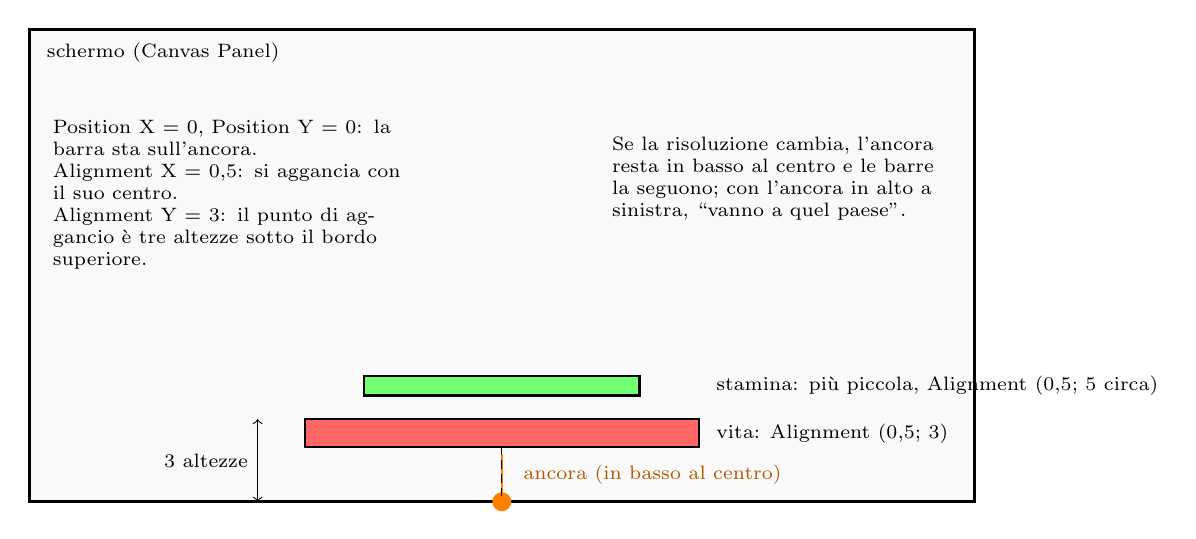
\begin{tikzpicture}[font=\footnotesize, x=1cm, y=1cm]
  % schermo
  \draw[very thick, fill=gray!5] (0,0) rectangle (12,6.0);
  \node[anchor=north west, font=\scriptsize] at (0.1,5.95) {schermo (Canvas Panel)};
  % ancora in basso al centro
  \fill[orange] (6,0) circle (0.12);
  \draw[orange, thick] (6,0) -- (6,0.6);
  \node[orange!70!black, font=\scriptsize, anchor=west] at (6.15,0.35) {ancora (in basso
    al centro)};
  % barra vita: alignment 0.5, 3 -> altezza 0.35 -> bordo superiore a 3*0.35=1.05
  \draw[thick, fill=red!60] (3.5,0.70) rectangle (8.5,1.05);
  \node[font=\scriptsize, anchor=west] at (8.6,0.87) {vita: Alignment (0,5; 3)};
  % barra stamina: posizione indicativa
  \draw[thick, fill=green!55] (4.25,1.35) rectangle (7.75,1.6);
  \node[font=\scriptsize, anchor=west] at (8.6,1.48) {stamina: più piccola, Alignment
    (0,5; 5 circa)};
  % pivot
  \draw[densely dashed] (6,0.70) -- (6,0);
  \draw[<->, thin] (2.9,0) -- node[left, font=\scriptsize]{3 altezze} (2.9,1.05);
  \node[font=\scriptsize, text width=4.6cm, align=left] at (2.6,3.9) {Position X = 0, Position
    Y = 0: la barra sta sull'ancora.\\ Alignment X = 0,5: si aggancia con il suo centro.\\
    Alignment Y = 3: il punto di aggancio è tre altezze sotto il bordo superiore.};
  \node[font=\scriptsize, text width=4.4cm, align=left] at (9.6,4.1) {Se la risoluzione
    cambia, l'ancora resta in basso al centro e le barre la seguono; con l'ancora in alto
    a sinistra, ``vanno a quel paese''.};
\end{tikzpicture}
\caption{Ancore, posizione e allineamento di un widget nel Canvas Panel. La posizione si
misura dall'ancora, l'allineamento sposta il punto dell'elemento che si aggancia
all'ancora, in frazioni della sua dimensione. Schema ricostruito; proporzioni indicative.}
\label{ue11:fig:ancore}
\end{figure}

\paragraph{Approfondimento: ancore e Percent nel libro.} Romero e Sewell (capitolo 7):
``poiché le dimensioni e i rapporti degli schermi possono variare, vogliamo assicurarci
che gli elementi della UI restino nella stessa posizione relativa sullo schermo. Le ancore
servono a definire la posizione desiderata di un widget sul canvas, indipendentemente
dalla dimensione dello schermo.'' Il simbolo a forma di fiore che si vede nel Designer si
chiama \emph{Anchor Medallion}, ``e rappresenta la posizione dell'ancora dell'elemento
selezionato''; la seconda edizione aggiunge che si può anche trascinare direttamente il
fiore nel punto voluto, o espandere \emph{Anchors} per i controlli di precisione. Uno dei
quesiti di fine capitolo chiede se ``i valori X e Y della posizione di un elemento in un
canvas sono sempre relativi all'angolo in alto a sinistra dello schermo'': la risposta è
no, sono relativi all'ancora, che è esattamente ciò che Guido ha scoperto. Sul Percent:
``l'intervallo dei valori va da 0,0 (vuota) a 1,0 (piena)''. Il libro anticipa anche il
motivo per cui serve una divisione: le sue variabili di vita e stamina hanno valore di
default 1,0 proprio perché ``questo valore è usato dai UI meters, che mostrano il grado di
riempimento fra 0,0 e 1,0''. La lezione invece tiene la vita in punti (10) e la stamina in
centesimi (100), e converte al momento di disegnare.

% ---------------------------------------------------------------------
\section{L'HUD sullo schermo: Initialize, Create Widget e Add to Viewport}
\label{ue11:sec:viewport}

\paragraph{L'evento d'inizializzazione.} Nel \textbf{Graph} del widget (``in alto a
destra, Designer e Graph: se clicchi su Graph vai direttamente là''), si tolgono gli eventi
predefiniti e si crea un \textbf{Custom Event}: \textbf{InitializeHealthBar}. Gli serve un
input, ``la referenza stessa al player'': nei Details dell'evento, sotto \emph{Inputs}, il
più, nome \textbf{PlayerRef}, tipo la classe del proprio personaggio (``io ho BP\_Bot2,
ma deve essere il nome del vostro character''), \textbf{Object Reference}: ``quella
azzurra, deve essere azzurra''. A che serve? ``Chiamerà l'Event Dispatcher'': il personaggio
dirà ``ehi, fammi esistere questa UI, mettimela sullo schermo'', e a quel punto bisogna
``bindare l'evento al fatto di inizializzare la barra, quindi dargli subito il valore di
quant'è la vita''. (A chi chiede ``com'è che sotto c'è la freccia bianca?'': è l'evento con
il suo input, che si aggiunge dai Details.)

\paragraph{Il Begin Play del personaggio.} ``Innanzitutto, buona regola, dobbiamo passargli
la PlayerRef.'' In BP\_Bot2, all'\textbf{Event BeginPlay}: ``quando il gioco inizia,
vogliamo che l'HUD, quindi questa schermata, la sua Progress Bar e tutto quanto, vada a
esistere nel mondo, nella nostra viewport''.
\begin{enumerate}
  \item \textbf{Create Widget} (``scusate, non \emph{Add}: è Create Widget''). Il pin
        \textbf{Class} chiede ``la tipologia di asset che andiamo a creare'': WB\_HUD;
  \item il \textbf{Return Value} si promuove a variabile, \textbf{AsHUD}: ``non lo useremo,
        però è una buona cosa sempre fare una referenza, perché magari volete comunicare
        altre volte con il nostro HUD e cambiargli dei valori'';
  \item ``questo lo crea, ma non lo mette nella viewport'': serve \textbf{Add to Viewport},
        con l'HUD come target. In Play, ``ecco a voi che la nostra barra rossa è apparsa
        a schermo'';
  \item infine, dalla variabile AsHUD, la chiamata a \textbf{InitializeHealthBar}, con
        \textbf{PlayerRef} collegato a un \textbf{Get a Reference to Self} (``fate
        \emph{self}, vi appare Get a Reference to Self''). ``Abbiamo detto: ehi, aggiungi
        questo widget alla viewport e inizializza.''
\end{enumerate}
(Durante questa parte il docente ha qualche problema di connessione: ``scusa, ho visto
adesso la chat; sto avendo problemi, devo fare un po' di manutenzione''.)

% ---------------------------------------------------------------------
\section{Il collegamento: Bind Event e Set Percent}
\label{ue11:sec:bind}

\paragraph{Il Bind.} ``Ci manca ovviamente la funzione collegata'': bisogna fare in modo
che l'inizializzazione \emph{agganci} l'aggiornamento della barra all'aggiornamento della
vita. Nel Graph del widget, dopo InitializeHealthBar, dal pin PlayerRef: \textbf{Bind
Event to E\_UpdateHealth} (la trascrizione sente ``bind e update''). Compilando dà errore,
``giustamente'': ``mi serve un evento: che evento devo collegare al fatto che io aggiorno la
mia variabile Health?''. L'evento si crea così: dal pin rosso \textbf{Event} del Bind si
trascina un filo e si sceglie \textbf{Add Custom Event}. ``Mi raccomando: non fate un
Custom Event esterno, tirate fuori proprio da Event e fate Custom Event, perché vi tira
fuori e si porta dietro i due valori che gli abbiamo dato di input, cioè CurrentHealth e
MaxHealth.'' Il nome: \textbf{UpdateHealthBar}.

\paragraph{Che cosa succede.} Una studentessa riassume: ``quindi quando viene
inizializzato, in automatico fa anche Update Health?''. ``Esatto.'' Quando il gioco
inizia, l'HUD ``binda l'evento di aggiornare la barra al nostro Update Health, cioè al
valore numerico che si aggiorna''. ``Creiamo il collegamento'': da quel momento, ``quando si
aggiorna effettivamente il nostro numero, la nostra variabile, allora avviene anche
l'update della barra''.

\paragraph{L'evento senza posti.} ``A me il Bind Event non me l'ha dato'': la studentessa
aveva creato prima, per sbaglio, un Custom Event separato e l'aveva collegato al Bind;
cancellato quello, il Bind risultava ``ancora delegato''. ``Elimina quello che hai
adesso; tira fuori da Event, Custom Event.'' La spiegazione: un Custom Event creato a mano
``non ti dà quei valori di input, CurrentHealth e MaxHealth''; ``questo qua deve essere
creato tramite il collegamento, perché noi gli abbiamo messo degli input''. ``Non deve
essere vuoto: si deve portare dietro i posti per la CurrentHealth e la MaxHealth.
Ricordiamoci il camion.''

\paragraph{Rinominare la barra.} ``Per ordine'': nel Designer, nella \textbf{Hierarchy}
(``ci permette di avere tutte le nostre cosine che abbiamo messo nella UI, tutte belle
elencate''), si seleziona la Progress Bar e con \textbf{F2} la si rinomina
\textbf{ProgressBar\_Health}.

\paragraph{Set Percent.} Nel Graph, la variabile ProgressBar\_Health si trascina
nell'evento UpdateHealthBar e da lei si tira fuori \textbf{Set Percent}. ``In questo caso
però si tratta di una percentuale, quindi è un valore da 0 a 1'': il valore è
\textbf{CurrentHealth diviso MaxHealth}, i due pin dell'evento in un \textbf{Divide}. In
Play, ``la mia barra diminuisce sempre di più, e boom, eccoci qua''
(figure~\ref{ue11:fig:hudgraph} e~\ref{ue11:fig:catena}).

\begin{figure}[htbp]
\centering
\begin{tikzpicture}[font=\scriptsize,
  ue11node/.style={draw, thick, rounded corners=4pt, align=center, fill=gray!8,
                  minimum height=0.9cm, text width=2.0cm},
  ue11ev/.style={ue11node, fill=red!12},
  ue11var/.style={ue11node, fill=blue!10, rounded corners=8pt},
  ue11exec/.style={-{Stealth[length=2.5mm]}, very thick, black!80},
  ue11data/.style={-{Stealth[length=2mm]}, thick, blue!60!black}]
  \node[font=\scriptsize\bfseries, anchor=west] at (-1.0,1.0) {BP\_Bot2, Event Graph};
  \node[ue11ev, text width=1.5cm] (bp) at (0,0) {\textbf{Event BeginPlay}};
  \node[ue11node, text width=1.7cm] (cw) at (2.4,0) {\textbf{Create Widget}\\Class:
    WB\_HUD};
  \node[ue11var, text width=1.4cm] (sh) at (4.7,0) {\textbf{Set}\\AsHUD};
  \node[ue11node, text width=1.6cm] (av) at (6.9,0) {\textbf{Add to Viewport}};
  \node[ue11node, fill=yellow!20, text width=2.5cm] (ih) at (9.7,0)
    {\textbf{Initialize\-Health\-Bar}\\PlayerRef: Self};
  \node[ue11node, fill=yellow!20, text width=2.5cm] (is) at (13.0,0)
    {\textbf{Initialize\-Stamina\-Bar}\\PlayerRef: Self (più tardi)};
  \draw[ue11exec] (bp) -- (cw); \draw[ue11exec] (cw) -- (sh);
  \draw[ue11exec] (sh) -- (av); \draw[ue11exec] (av) -- (ih);
  \draw[ue11exec, dashed] (ih) -- (is);
  \node[font=\scriptsize\bfseries, anchor=west] at (-1.0,-1.6) {WB\_HUD, Graph};
  \node[ue11ev, text width=2.5cm] (ini) at (0.3,-2.7) {\textbf{Initialize\-Health\-Bar}\\
    Custom Event, input PlayerRef};
  \node[ue11node, text width=2.5cm] (bind) at (3.9,-2.7) {\textbf{Bind Event to
    E\_UpdateHealth}\\Target: PlayerRef};
  \node[ue11ev, text width=2.5cm] (upd) at (8.3,-2.7) {\textbf{Update\-Health\-Bar}\\
    CurrentHealth, MaxHealth};
  \node[ue11node, text width=1.6cm] (div) at (10.9,-4.4) {\textbf{Divide}\\Current /
    Max};
  \node[ue11node, text width=2.6cm] (sp) at (12.4,-2.7) {\textbf{Set Percent}\\Target:
    ProgressBar\_Health};
  \draw[ue11exec] (ini) -- (bind);
  \draw[ue11data, red!60!black] (bind) -- node[below]{Event} (upd);
  \draw[ue11exec] (upd) -- (sp);
  \draw[ue11data] (upd.south) |- (div.west);
  \draw[ue11data] (div.north) -- node[right]{In Percent} (sp.south -| div.north);
\end{tikzpicture}
\caption{I due lati dell'HUD. In alto, il personaggio crea il widget, se lo salva, lo
aggiunge alla viewport e gli passa una referenza a se stesso. In basso, il widget usa
quella referenza per legare il proprio evento UpdateHealthBar all'Event Dispatcher del
personaggio: da lì in poi, ogni Call E\_UpdateHealth esegue Set Percent. La chiamata
tratteggiata si aggiunge con la stamina. Schema ricostruito.}
\label{ue11:fig:hudgraph}
\end{figure}

\begin{figure}[htbp]
\centering
\begin{tikzpicture}[font=\footnotesize,
  ue11node/.style={draw, thick, rounded corners=4pt, align=center, fill=gray!8,
                  minimum height=1.0cm, text width=2.5cm},
  ue11exec/.style={-{Stealth[length=2.5mm]}, very thick, black!80}]
  \node[ue11node, fill=orange!15] (pr) at (0,0) {\textbf{BP\_Projectile}\\{\scriptsize
    Sphere Trace, Break Hit Result}};
  \node[ue11node, fill=orange!15] (ad) at (3.4,0) {\textbf{Apply Damage}\\{\scriptsize
    Hit Actor, Base Damage 1}};
  \node[ue11node, fill=red!12] (any) at (6.8,0) {\textbf{Event Any\-Damage}\\{\scriptsize
    in BP\_Bot2}};
  \node[ue11node, fill=blue!10] (hp) at (10.2,0) {\textbf{CurrentHealth}\\{\scriptsize
    Subtract, Clamp, Set}};
  \node[ue11node, fill=yellow!20] (call) at (10.2,-2.2) {\textbf{Call
    E\_UpdateHealth}};
  \node[ue11node, fill=green!10] (ev) at (6.8,-2.2) {\textbf{Update\-Health\-Bar}\\
    {\scriptsize in WB\_HUD (legato)}};
  \node[ue11node, fill=green!10] (pb) at (3.4,-2.2) {\textbf{Set Percent}\\{\scriptsize
    Current / Max}};
  \node[ue11node, fill=green!20] (bar) at (0,-2.2) {\textbf{barra rossa}\\{\scriptsize
    sullo schermo}};
  \draw[ue11exec] (pr) -- (ad); \draw[ue11exec] (ad) -- (any);
  \draw[ue11exec] (any) -- (hp); \draw[ue11exec] (hp) -- (call);
  \draw[ue11exec] (call) -- (ev); \draw[ue11exec] (ev) -- (pb);
  \draw[ue11exec] (pb) -- (bar);
  \node[font=\scriptsize, text width=13cm, align=center] at (5.1,-3.6) {Il proiettile non
    sa nulla della UI, e la UI non sa nulla del proiettile: ognuno parla solo con il
    personaggio.};
\end{tikzpicture}
\caption{Il percorso completo di un colpo, dal proiettile alla barra. Il sistema di danno
di Unreal collega il proiettile al personaggio; l'Event Dispatcher collega il personaggio
all'HUD. Schema riassuntivo.}
\label{ue11:fig:catena}
\end{figure}

\paragraph{I problemi dei presenti.} ``Ci siete, ragazzi?'' Tre casi.
\begin{itemize}
  \item \textbf{Set Percent introvabile.} ``Non mi dà il Set Percent'', e nemmeno i
        Details per cercarlo. Primo controllo: nel Designer, la Progress Bar deve avere la
        spunta \textbf{Is Variable}, altrimenti nel Graph non esiste come variabile. I
        Details mancanti si riaprono da \textbf{Window}, \textbf{Details}. La spunta c'era;
        il vero errore è un altro: lo studente cercava Set Percent trascinando da un altro
        nodo. ``Ah, ok, lo facevo da qua'': Set Percent si trova solo \emph{tirando fuori
        dalla variabile} ProgressBar\_Health, che va presa dalla sezione \emph{Variables}
        (``se non ce l'hai, c'è la tendina'') e trascinata nel grafo. Per la divisione:
        ``tiri fuori dalla CurrentHealth e fai lo slash'', oppure si scrive
        \emph{divide}; poi ``questo diviso per quell'altro''.
  \item \textbf{La torretta che non spara}, a un'altra studentessa: rimandata alla pausa.
  \item \textbf{La barra che non scende.} ``La vita la perdo, perché poi respawno; tuttavia
        graficamente non scende la barra.'' Il Bind c'è, il danno è 1 (``l'ho messo come
        variabile''), la vita è 10. Un Print String dopo il Set Percent, ``attaccalo a In
        String'' (``collega quello verde a quello rosa''), non stampa niente. Allora
        \textbf{F9} sull'evento UpdateHealthBar: ``dice: sta facendo questo evento?''. Il
        breakpoint non scatta. In BP\_Bot2 si scopre perché: nel Begin Play mancava la
        chiamata a \textbf{InitializeHealthBar} dopo Add to Viewport. ``Non stai dicendo al
        gioco che, quando inizia, se io ho dato la vita, mi aggiorni pure la barra.'' Si
        aggiunge da AsHUD, con Self nel PlayerRef; si toglie il breakpoint (``se no te lo
        farà ogni volta''). ``Perfetto, grazie.''
\end{itemize}

\paragraph{Il portatile surriscaldato.} Un altro studente non riesce a seguire: ``sta
andando a scatti'', ``è troppo surriscaldato il computer''. Il consiglio, per tutti: ``per
chi ha un portatile, prendetevi quelle basette con le ventole'': ``col portatile quello
diventa un vulcano a un certo punto''. Lo studente ce l'ha già: ``ah, ok. Quindi sta proprio
andando pesantissimo''. ``Lascialo riposare il nostro soldato, tranquillo: tanto poi c'è la
registrazione.''

\paragraph{Approfondimento: Bind Event contro i Binding del libro.} Qui la lezione e il
libro scelgono due strade diverse, e vale la pena capire perché. Romero e Sewell
(capitolo 7) usano i \textbf{Binding} delle proprietà: accanto al campo \emph{Percent}
della Progress Bar c'è un pulsante \emph{Bind}; scegliendo \emph{Create Binding}, l'editor
crea una funzione che restituisce il valore, in cui gli autori mettono \emph{Get Player
Character}, \emph{Cast To FirstPersonCharacter} e il Get della vita. ``I Binding ci danno
la possibilità di legare variabili o funzioni di un Blueprint a un Widget. Ogni volta che
la variabile o la funzione è aggiornata, il cambiamento si riflette automaticamente nel
Widget.'' Il prezzo, per il funzionamento generale di UMG, è che una funzione di Binding
viene valutata \emph{a ogni frame}, che il valore sia cambiato o no (e, nell'esempio del
libro, con un cast a ogni valutazione). Lo schema della lezione è \emph{a eventi}: la barra
si aggiorna solo quando il personaggio chiama E\_UpdateHealth, cioè quando la vita cambia
davvero. Per due barre la differenza di prestazioni è trascurabile; diventa importante
negli HUD con molti elementi, e soprattutto rende esplicito \emph{chi} aggiorna \emph{che
cosa}. Sul Bind Event, invece, il libro (capitolo 4) dice la stessa cosa del docente:
``c'è un nodo Bind Event che lega un evento a un altro evento o a un Event Dispatcher, che
può stare in un altro Blueprint. Quando un evento è chiamato, tutti gli altri eventi legati
a lui sono chiamati'', e il Custom Event si crea trascinando ``dal pin rosso del nodo Bind
Event'' e scegliendo \emph{Add Custom Event}. Un dettaglio generale: un Custom Event creato
dal pin riceve automaticamente la \emph{firma} del dispatcher (i suoi input); se in seguito
si aggiungono input al dispatcher, gli eventi legati vanno aggiornati, e l'editor lo segnala
con un errore di firma alla compilazione.

% ---------------------------------------------------------------------
\section{La seconda barra e la corsa}
\label{ue11:sec:corsa}

``Abbiamo un quarto d'oretta. Sai che facciamo? Andiamo a creare la nostra barra della
stamina e facciamo insieme la stamina, così dopo magari facciamo qualcos'altro, che è il
menu in questo caso.''

\paragraph{La barra copiata.} ``Più che metterne una nuova'', nel Designer di WB\_HUD si
copia la barra della vita con \textbf{Ctrl+C} e \textbf{Ctrl+V}. La copia ha ancora
l'ancora in basso al centro; si azzerano le posizioni, \textbf{Alignment} X a \textbf{0,5}
e Y più alto, perché stia sopra la barra rossa (il docente dice ``non 3, ma la mettiamo
tipo a 2, e facciamo 5'', poi ``facciamo 5''), la si fa ``un pochino più piccola'' (con i
campi della dimensione, ``1,8, ma sì, 2'': ``questi rettangolini servono per essere un po'
più precisi''), e verde. ``Se volete, ragazzi, sbizzarritevi: i colori, proprio pastelli in
mano, fate come volete.''

\paragraph{InitializeStaminaBar.} ``Facciamo la stessa identica cosa per l'inizializzazione
della barra'': nel Graph, un altro Custom Event, \textbf{InitializeStaminaBar}, con lo
stesso input \textbf{PlayerRef} (``fortunatamente, se avete già fatto l'input, vi dice già:
ce l'ho, PlayerRef''). ``Per adesso lo lasciamo così, perché dobbiamo creare un altro
Event Dispatcher, che sarà invece l'update della stamina.''

\paragraph{IA\_Run.} Torniamo nel bot: ``dobbiamo far correre il nostro player''. Serve
un'\textbf{Input Action} nuova, \textbf{IA\_Run}, accanto a IA\_Look, IA\_Move e IA\_Jump;
la si era fatta la volta scorsa per il cavaliere, e ``fortunatamente'' basta una volta:
``questa è la bellezza del context: la mappatura degli input è separata dal player'', e
``la posso passare da player a player''. Per chi non ce l'ha:
\begin{enumerate}
  \item da un'azione qualsiasi, tasto destro, \textbf{Show in Folder View}; si
        \textbf{duplica} IA\_Jump e la si chiama IA\_Run. ``Se non sbaglio, Jump e Run
        sono uguali'': entrambe hanno un valore booleano (\emph{Digital});
  \item nell'\textbf{IMC} (\emph{Input Mapping Context}), il più, IA\_Run, e nella
        tendina la \textbf{tastiera}: ``cliccate sulla tastiera, premete Shift'', ``in modo
        da dire: guarda che questo è l'input collegato alla corsa''.
\end{enumerate}
``Io l'ho spiegato molto velocemente, perché so che, se qualcuno nel caso non avesse
visto, poi mi dica.''

\paragraph{Gli stati dell'evento.} Nel bot, l'evento \textbf{IA\_Run} mostra le sue uscite
(\emph{Triggered}, \emph{Started}, \emph{Ongoing}, \emph{Canceled}, \emph{Completed});
``in questo caso ci interesseranno solamente lo \textbf{Started} e il
\textbf{Completed}'': l'inizio e la fine della pressione.

\paragraph{Camminare di default.} ``Per dire già che il player deve camminare di default'',
si guarda il Blend Space del bot: la camminata è a 250, ``facciamo 300, un po' più alto''.
Nel \textbf{Character Movement}, categoria \emph{Character Movement: Walking},
\textbf{Max Walk Speed} a \textbf{300}: ``da adesso in poi il nostro character camminerà''.
(Se i passi non suonano, ``lo fixiamo poi'': il docente aveva aggiunto i suoni dei passi
anche all'animazione di camminata prima della lezione, ``perché prima solamente
correvamo''.)

\paragraph{Correre.} Due \textbf{Set Max Walk Speed}, entrambi con il Character Movement
come target (``ricordatevi di tutti e due di collegarli''): uno allo \textbf{Started}, a
\textbf{500}, uno al \textbf{Completed}, a \textbf{300}. (Il docente dice prima 600, poi
``500 era? Facciamo 500, va bene'', il valore massimo del Blend Space.) In Play: ``cammino;
Shift, corro; Shift, lascio''. ``Sicuramente possiamo mettere un po' di smooth
all'animazione'', con un \emph{blend in} e un \emph{blend out}: ``questo è un fix che
possiamo fare dopo, tranquillamente''.

\paragraph{La stamina di Dark Souls.} ``Qualcuno di voi ha in mente Dark Souls? La stamina
di Dark Souls, o in generale, molto spesso la stamina funziona in questo modo'': ``viene
persa durante un quantitativo di tempo, se si fa una certa azione, in questo caso correre:
viene levata gradualmente'', e quando l'azione smette ritorna su piano piano. ``Visto che
parliamo di tempo, useremo due \textbf{timer}'', come per la torretta, ``per far sì che
queste due cose vadano a scalare nel tempo''. Mancano cinque minuti alla pausa: ``facciamo
adesso un piccolo timer, oppure vogliamo andare già in pausa?''. Si va in pausa: ``la
prova è 25'', ``facciamo 17 e 55 e ci rivediamo''.

\paragraph{Approfondimento: lo sprint nel libro.} Romero e Sewell costruiscono lo sprint nel
capitolo 6 con il sistema di input precedente (l'\emph{Action Mapping} ``Sprint'' sul
tasto Shift sinistro, gli eventi \emph{Pressed} e \emph{Released}) e due \emph{Set Max
Walk Speed}, esattamente come la lezione con l'Enhanced Input (Started e Completed). Nel
capitolo 8 fanno un'osservazione di design che spiega perché la stamina serve: senza un
vincolo, ``non ci sarebbe niente a scoraggiare il giocatore dal tenere sempre premuto
Shift mentre si muove''; ``se un'opzione è così attraente che il giocatore si sente
costretto a usarla sempre, allora non aumenta il numero di scelte interessanti''. ``Dal
punto di vista del giocatore, il risultato sarebbe lo stesso se aumentassimo semplicemente
la velocità di base fino a quella dello sprint.'' La stamina trasforma lo sprint in una
\emph{risorsa}: correre ora significa non poter correre fra poco. È la stessa logica della
stamina di Dark Souls, dove la stessa barra è condivisa da corsa, schivata, parata e
attacco, e ogni scelta ha un costo.

% ---------------------------------------------------------------------
\section{La pausa: le torrette e i bot degli studenti}
\label{ue11:sec:pausa}

La pausa, come spesso in questo corso, diventa uno sportello di correzioni. Il docente
resta collegato e guarda i progetti uno alla volta, in condivisione di schermo
(``quando condividi, fai \emph{condividi schermo}, non condividere Unreal, perché è più
facile: stiamo schermando più grande'').

\paragraph{Lo Shift che non corre.} Il primo studente: ``se mi muovo normalmente cammina,
se premo Shift non corre''. ``Allora c'hai qualche cosa che non va nell'IA\_Run.'' La cosa
resta in sospeso: il problema dello stesso tipo tornerà, più grave, alla fine della lezione
(sezione~\ref{ue11:sec:barrastamina}).

\subsection{La torretta di Tommaso}

``Io entro, mi vede, ma non spara.'' Il tag Player c'è.
\begin{enumerate}
  \item \textbf{La collisione della mesh del bot}: ``non l'avevo messa''. Mesh, Collision,
        Custom, Detection Turret in Block (e Projectile Trace: ``va benissimo''). Ora la
        torretta lo segue, ma non spara.
  \item \textbf{Il Trace Channel}: nella torretta, il trace di rilevamento usava il canale
        sbagliato. ``Cambia Trace Channel'' a \textbf{Detection Turret} (``no, no, torna
        indietro; Ctrl+Z''). ``Ok, benissimo.''
  \item \textbf{La funzione dello spawn}: alla torretta di Tommaso manca proprio la
        funzione che fa nascere il proiettile. Il docente gliela passa con ``un
        trucchettino'': ``la cosa bella dei Blueprint è che puoi incollarli in un file di
        testo, copiarli tutti quanti''. Seleziona i nodi della sua funzione, Ctrl+C, li
        incolla in un file \emph{.txt} (``Fix, funzione Spawn'') e glielo manda su
        Discord, in privato. Tommaso scarica il file, ne copia tutto il testo e lo incolla
        con Ctrl+V nel grafo di Unreal: i nodi ricompaiono.
  \item \textbf{Sistemare l'incollato}: ``adesso c'hai degli errori, eh? Perché devi
        sistemarlo''; ``prima fix, poi ordina''. La funzione si rinomina con F2
        \textbf{Spawn Projectile}. Servono i due punti di uscita: nei Components, Add,
        due \textbf{Scene Component}, \textbf{ProjectileSpawn1} e \textbf{ProjectileSpawn2}
        (copiati con Ctrl+C e Ctrl+V), agganciati al \textbf{cannone} della torretta e
        spostati ``ai bocchettoni della mesh'', ``poco fuori la canna''.
  \item \textbf{Lo Spawn Actor rifatto}: il nodo incollato dà un errore sull'\emph{Spawn
        Actor} (``non ti spawno nessun actor''); l'errore sull'\emph{Instigator} invece
        ``va bene, non ci interessa''. ``Facciamo prima'': si cancella e si rifà
        \textbf{Spawn Actor from Class}; tasto destro sullo \emph{Spawn Transform},
        \textbf{Split Struct Pin}; si collegano Location e Rotation dei due Scene; la
        \textbf{Class} è il proiettile, BP\_Projectile.
  \item Una curiosità di Tommaso, nel frattempo: ``pure la barra della stamina, io gli ho
        dato un colore, ma me la dà grigia''. ``Forse è vuota'': il \emph{Percent} è a 0,
        e una Progress Bar vuota mostra solo lo sfondo. ``Faccio 1.''
  \item \textbf{Chiamare la funzione}: la torretta ancora non spara, ``perché non
        spawni'': nello \emph{Shoot}, al posto delle due vecchie chiamate, va chiamata la
        nuova \textbf{Spawn Projectile}.
  \item \textbf{Le collisioni della torretta}: il proiettile non deve fermarsi sulla
        torretta stessa. Sul cannone, sulla sfera di rilevamento e sul pivot, il canale
        Projectile Trace va su \textbf{Ignore} (``devi ignorare tutto, anche il pivot'').
\end{enumerate}
La torretta di Tommaso ancora non spara; ``aspetta, adesso facciamo fare Lucrezia, che è
un po' che aspetta''. Si riprenderà dopo la pausa.

\subsection{Il bot di Lucrezia, risolto}

\paragraph{Il Validated Get sulla variabile sbagliata.} Con Shift il bot di Lucrezia ora
``va più veloce'': ``quello almeno va benissimo''; quindi il personaggio si muove, ``è un
problema di animazioni''. Il docente esclude un doppio scheletro (``non vorrei che avessi
un doppio scheletro e te l'avessi fatto su un altro'': ne ha uno solo), poi mette un
Print String sull'uscita \textbf{Is Not Valid} del Validated Get, all'inizio dell'Update.
Stampa: ``ecco il nostro problema: la referenza a questo actor non è valida''. Il motivo:
``hai messo nel Validated Get la variabile del PB\_Bot, non del BP\_Bot, che sono due
diverse'': nell'Animation Blueprint c'erano due variabili quasi omonime, e il Validated
Get controllava quella che l'Initialize non riempiva mai. Si cancella, si prende la
variabile giusta (\textbf{AsBP\_Bot}), tasto destro, \textbf{Convert to Validated Get}, si
ricollega. ``Dovremmo aver scoperto l'arcano.'' ``Era lui.''

\paragraph{La regola di ritorno all'Idle.} Ora il bot anima, ma ``continua a camminare sul
posto'' quando si ferma. Nella State Machine, la regola Walk $\rightarrow$ Idle era
\emph{GroundSpeed $<$ 0}: ``attenzione, non è minore, è \textbf{minore o uguale}'',
perché una velocità negativa non esiste (la lunghezza di un vettore è sempre $\ge 0$), e con
il minore stretto la regola non è mai vera (``solo se sarà meno uno la velocità'').

\paragraph{Il Lean, di nuovo.} Correndo e girando, il bot ``non si inclina tantissimo'':
la stessa correzione fatta a inizio lezione (``come abbiamo fatto anche con Tommaso'': la
trascrizione attribuisce qui a Tommaso il Lean corretto all'inizio). Nel Blend Space i
campioni da $\pm 10$ a $\pm 1$, poi l'asse, nelle \emph{Axis Settings} dei Details, da $-1$
a 1. ``Ecco che si piega leggermente.''

\paragraph{La torretta di Lucrezia.} Poi la torretta, aperta con \emph{Edit BP\_Turret} dal
livello (``lo fai diretto''). ``Questo è un po' incasinato, eh? Vabbè, tranquillo.'' In
ordine:
\begin{itemize}
  \item \textbf{Begin Overlap}: il fix di inizio lezione, Get Player Pawn al posto
        dell'Other Actor nel Set di PlayerTarget;
  \item \textbf{Move Turret} (la rotazione verso il bersaglio): il nodo di rotazione
        usato era un altro, e si sostituisce con \textbf{Find Relative Look at
        Rotation}, che vuole uno \emph{Start Transform} (``non ti serve il Get Actor
        Rotation, ma devi invocare il \textbf{Get Actor Transform}'', ``pinnetto
        arancione per pinnetto arancione'') e una \emph{Target Location}, il \textbf{Get
        Actor Location} del PlayerTarget. Del risultato, con \emph{Split Struct Pin}, si
        usa la \textbf{Z} (lo Yaw) come \emph{Target} dell'interpolazione; un vecchio
        ``meno'' non serve più; nel \emph{Delta Time} va \textbf{Get World Delta Seconds}.
        La trascrizione, qui, è troppo frammentaria per ricostruire il grafo nodo per nodo;
        il senso è quello della rotazione della torretta costruita nelle lezioni
        precedenti;
  \item \textbf{Shoot}: Branch, Sequence, i due \emph{Do Once} con lo Spawn Projectile e il
        Delay, il \emph{Fire Rate}: ``va benissimo'';
  \item un secondo \emph{On Component Begin Overlap} rimasto da una prova (``probabilmente
        una cosa che avevo cancellato'', ``l'avevo spostata''): si elimina; l'\emph{End
        Overlap} e il Tick si tengono;
  \item \textbf{il tag}: la torretta ancora non la segue. Il tag Player era stato messo nei
        \emph{Component Tags} della mesh: ``attenzione, non della mesh, ma quello sotto'':
        i \textbf{Tags} dell'\emph{actor}, e con la stessa maiuscola.
\end{itemize}

\paragraph{Il proiettile assassino.} Ora la torretta spara (``sei un po' alta''), ma
emergono tre problemi del proiettile, uno dopo l'altro.
\begin{enumerate}
  \item I proiettili urtano la camera del personaggio: sulla \emph{Sphere} del proiettile,
        Collision, \textbf{Camera} su \textbf{Ignore}.
  \item I proiettili ``non si distruggono se il character gli va addosso'': la Sphere
        Trace aveva \textbf{Radius 0}, ``quindi è grande niente''. A \textbf{20}.
  \item Ora un colpo e il bot ``si blocca proprio tutto'', anche se la vita non è finita.
        Nel proiettile, dopo il colpo, c'era un \textbf{Destroy Actor} con l'\emph{Hit
        Actor} come target (un ramo chiamato \emph{Kill Target}): ``se colpisco qualcosa,
        distruggimi quello che ho colpito''. Il proiettile cancellava il personaggio dal
        mondo. Al suo posto: \textbf{Apply Damage} (Hit Actor nel Damaged Actor, Base
        Damage 1), e poi \textbf{Destroy Actor} senza target, cioè \emph{self}: ``quando
        collide con qualcosa, distruggi il proiettile: si autodistrugge''.
\end{enumerate}

\paragraph{La vita a zero e la NewVar.} Ora il bot ``muore praticamente subito'': la
\textbf{MaxHealth} aveva default 0, e il Clamp riduceva a zero qualunque vita. MaxHealth a
10. Poi il contrario: il primo colpo toglie vita, ``poi adesso è immortale''. Nell'Event
AnyDamage c'era un Set su una variabile \textbf{NewVar}, creata per sbaglio, invece che
sulla CurrentHealth: ``stai praticamente mettendo una variabile nuova come vita''. Si
sostituisce con \emph{Set CurrentHealth}, ricollegando il Return Value del Clamp e il
valore al Branch del minore o uguale. ``Perfetto. Grazie mille.''

\paragraph{Approfondimento: i Blueprint come testo.} Il ``trucchettino'' del file di testo
funziona perché Unreal copia i nodi negli appunti in un formato testuale (lo stesso
formato \emph{T3D} usato per copiare gli actor fra livelli): ogni nodo diventa un blocco
\texttt{Begin Object} \dots\ \texttt{End Object} con la sua classe, la posizione nel grafo,
i valori dei pin e i collegamenti. Incollando quel testo in un altro grafo, anche di un
altro progetto, l'editor ricrea i nodi. È il modo più rapido per condividere un pezzo di
logica in chat o su un forum, ed esistono siti che lo visualizzano come immagine. Il
limite è quello visto a lezione: i riferimenti a variabili, componenti e funzioni del
Blueprint d'origine non esistono nel Blueprint di destinazione, e i nodi che li usano
arrivano ``rotti'' e vanno ricollegati o ricreati (come gli Scene Component e lo Spawn
Actor di Tommaso). Questa è una nozione generale dell'editor, non trattata nei due libri.

% ---------------------------------------------------------------------
\section{Dopo la pausa: ancora la torretta, e gli annunci}
\label{ue11:sec:annunci}

``Eccoci qua, ragazzi, siamo ritornati.'' Tommaso ha provato a togliere e rimettere la
torretta: niente.

\paragraph{L'Event Tick che manca.} ``Io credo che sia \emph{not valid} il PlayerTarget,
probabilmente.'' Il Begin Overlap e il timer sono giusti; ``ah, ti manca il Tick''.
Nell'Event Graph della torretta non c'è l'\textbf{Event Tick} che, a ogni frame, controlla
il bersaglio e spara. Si ricrea: Event Tick, \textbf{Is Valid} (``punto interrogativo,
quello sotto'') con il PlayerTarget come oggetto, e sull'uscita \emph{Is Valid} la
funzione \textbf{Shoot}. La torretta spara.

\paragraph{Fire Rate e velocità.} ``È un po' lento a sparare'': il \textbf{Fire Rate}, fra
le variabili della torretta, è a 0,2 (la trascrizione dice ``02''); il docente suggerisce
un altro valore (``facciamolo 0,7''; il suo è 0,5): dalla trascrizione non si capisce se
il valore sia un intervallo fra i colpi o un'altra cosa nel grafo di Tommaso, e il capitolo
non lo ricostruisce. ``Il proiettile è molto lento'': nel proiettile, il componente
\textbf{Projectile Movement}, \textbf{Initial Speed} e \textbf{Max Speed} a \textbf{1000}.

\paragraph{Il danno che non arriva alla barra.} ``Però non prendo danno.'' Il proiettile ha
l'Apply Damage, ``va bene così''; nel BP\_Bot, però, l'\textbf{Add to Viewport} non era
collegato con il pin di esecuzione all'InitializeHealthBar (``vedi che non è stato
attaccato''). E non basta: nell'Event AnyDamage il Set era su \textbf{MaxHealth} invece che
su CurrentHealth (``ha impostato MaxHealth, non CurrentHealth''). Corretti entrambi:
``vediamo se muoio''. ``Ottimo, perfetto: di solito tutto il casino.''

\paragraph{Il calendario.} Prima di riprendere, gli annunci.
\begin{itemize}
  \item Il \textbf{menu}: ``se non ce la facciamo a fare il menu oggi, lo facciamo la
        prossima volta, e tanto la prossima volta sarà l'ultima lezione che avremo''.
  \item Dopo: ``poi avrete Davide, quindi avrete martedì con me e Davide''; ``poi
        inizierete a fare roba di \textbf{level design}''.
  \item Manca ``un piccolo asset da fare'', le \textbf{porte}: ``possiamo farlo
        tranquillamente la prossima volta, o ve lo lascio come compito, perché sono sicuro
        che lo sapete fare''. ``La timeline l'abbiamo già affrontata'' (il compito è
        descritto nella sezione~\ref{ue11:sec:chiusura}).
\end{itemize}
(``Non stai condividendo?'' ``Ah, ok. Grazie mille, Lucrezia.'')

% ---------------------------------------------------------------------
\section{I due timer della stamina}
\label{ue11:sec:timer}

``E adesso incominciamo a fare questo bellissimo scattino.'' Si torna al bot del docente
(``il proiettile non ci serve più; ci serve botolino''). Il movimento c'è già (500 e 300
sull'IA\_Run); ``abbiamo detto che dobbiamo fare due timer ben distinti: uno che la consuma
e uno che la riporta al suo massimo, piano piano nel tempo''.

\subsection{Il timer che consuma}

\paragraph{Set Timer by Event.} Dopo il Set Max Walk Speed a 500 (lo Started), un
\textbf{Set Timer by Event}.
\begin{itemize}
  \item il pin \textbf{Time} si promuove a variabile, \textbf{TimeStamina}, ``in modo tale
        da avere questa variabile molto più controllabile''; default \textbf{0,05}
        (impostato poco dopo: ``piccola cosa, semplicemente non l'abbiamo impostato''):
        ``questo è il tempo in cui verrà eseguito il timer, ogni 0,05 secondi'';
  \item \textbf{Looping} attivo; \textbf{Max Once Per Frame} attivo;
  \item ``il timer, come abbiamo visto le scorse volte, è un evento collegato'': dal pin
        rosso \textbf{Event} si crea un Custom Event, \textbf{StaminaDeduction}.
\end{itemize}

\paragraph{Le variabili.} ``Lo stesso discorso vale come per la Health'': due Float,
\textbf{CurrentStamina} e \textbf{MaxStamina}, entrambe a \textbf{100}.

\paragraph{StaminaDeduction.} Il corpo è quasi identico a quello della vita:
\begin{enumerate}
  \item CurrentStamina \textbf{Subtract} \textbf{1} (``verrà sottratto di 1 ogni 0,05
        secondi'');
  \item \textbf{Clamp (float)}, fra 0 e MaxStamina (``il nostro valore oscillerà fra un
        minimo di 0 e un massimo di MaxStamina, che è 100'');
  \item \textbf{Set CurrentStamina}: ``farà 99, 98, 97\dots''.
\end{enumerate}
``Questo è lo stesso discorso che vale per la Health, è quasi praticamente medesimo.''

\paragraph{Quando fermarsi: OR con Is Falling.} Poi un \textbf{Branch} (``tenete proprio
B'' e cliccate: la scorciatoia del Branch): se la CurrentStamina è \textbf{minore o uguale
a zero}, si fermerà la corsa (``ancora non abbiamo la funzione, ma la lasciamo così''). E
una piccola accortezza nata ``durante il testing'': ``ci sono dei problemi anche nel caso
noi stiamo cadendo''. ``Io tengo premuto il tasto mentre sto cadendo: non voglio che la
stamina venga consumata, perché non stiamo correndo effettivamente.'' Dal Character
Movement, \textbf{Is Falling} (``ce ne sono due: prendete quello \emph{Nav Movement}'',
quello con l'ingresso blu e l'uscita rossa), e i due booleani in un \textbf{OR Boolean}:
``OR è l'operatore che ci permette di dire \emph{o}: ti fermi se sei minore di zero
\emph{o} se stai cadendo'' (figura~\ref{ue11:fig:deduction}).

\paragraph{Il timer che non si ferma.} Con un Print String della CurrentStamina: ``io
cammino, cammino, comincio a sprintare: i valori scendono. Ma se anche smetto di correre,
i valori continuano a scendere, perché non stoppiamo mai il nostro timer.'' La soluzione è
tenere un \emph{riferimento} al timer: il \textbf{Return Value} di Set Timer by Event (un
\emph{Timer Handle}) si promuove a variabile, \textbf{TimerDeductionStamina}, ``in modo tale
che sia più comodo controllarlo da varie parti''. Al \textbf{Completed} dell'IA\_Run, dopo
il Set Max Walk Speed a 300: un Get di TimerDeductionStamina e \textbf{Clear and Invalidate
Timer by Handle}, ``andiamo a invalidare e fermare il nostro timer''. In Play: ``corro,
smetto di correre: si è fermato a 75''.

\subsection{Il timer che ricarica}

\paragraph{Il secondo timer.} ``Altro problema: se io ricomincio a correre, ripartirà da 75,
non torna piano piano verso 100.'' Quando si smette di correre bisogna ``fare l'opposto'':
subito dopo il Clear, un altro \textbf{Set Timer by Event}, ``sempre in Looping, sempre in
Max Once Per Frame''. Per il tempo il docente usa la stessa TimeStamina, ``ma volendo si può
fare a un valore che volete voi: volete che uno si recuperi più veloce oppure più lento,
sta a voi''. Il suo evento è un Custom Event, \textbf{RegainStamina}: ``non c'è neanche
tanto da sbizzarrirci: è letteralmente la copia di questo''. Si copiano i nodi della
deduzione fino al Set e ``l'unica cosa che andiamo a cambiare è che invece di sottrarre
uno, andiamo ad aggiungere uno'': \textbf{Add} 1, Clamp, Set CurrentStamina.

\paragraph{Fermare anche lui.} Stesso schema al contrario: il Return Value si promuove a
\textbf{TimerRegainStamina}, e allo \textbf{Started} (``quando noi ricominciamo a
correre'') un \textbf{Clear and Invalidate Timer by Handle} su di lui. In Play: ``comincio a
correre, i valori cominciano a scendere; lascio, i valori piano piano risalgono fino a
100''.

\paragraph{Fermarsi a 100.} Ma arrivato a 100, il timer della ricarica continua a girare,
inutilmente. In RegainStamina, dopo il Set, un \textbf{Branch}: se la CurrentStamina è
\textbf{maggiore o uguale} alla MaxStamina, un Clear and Invalidate Timer by Handle su
TimerRegainStamina, ``cioè lo stesso timer che stiamo avendo'': ``se arrivi a 100,
smettila''. ``Non stampo più, si è fermato.''

\subsection{L'evento StopRunning}

\paragraph{La corsa che non finisce.} ``C'è una particolarità'': correndo fino a zero, ``il
nostro character non si ferma, e neanche il timer si ferma'', e il personaggio continua a
correre con la stamina vuota. Serve la funzione di \emph{smettere di correre} anche
\emph{dentro} StaminaDeduction, non solo al rilascio del tasto. ``Per comodità, invece di
fare una funzione a parte'': si stacca il \textbf{Completed} dalla sua catena (Set Max Walk
Speed 300, Clear del timer di deduzione, Set Timer della ricarica), e all'inizio della
catena si mette un nuovo Custom Event, \textbf{StopRunning}. Poi:
\begin{itemize}
  \item il \textbf{Completed} chiama StopRunning;
  \item il ramo \textbf{True} del Branch di StaminaDeduction (stamina $\le$ 0 OR Is
        Falling) chiama StopRunning.
\end{itemize}
``Questa cosa ci serve semplicemente per trasportarci il fatto di \emph{fermati}: vai a
300 di velocità e smettila di sottrarmi la stamina, da questo evento che possiamo
trasportare un po' dappertutto.'' In Play: ``corro, corro, corro, arrivo fino a zero, mi
fermo in automatico'', la stamina risale; ``e poi devo semplicemente ripremere per poter
scattare'' (lo \emph{Started} scatta solo alla pressione). ``Abbiamo fatto il nostro
sistema di stamina'' (figura~\ref{ue11:fig:timer}).

\paragraph{Ricapitolare per chi si è perso.} Una studentessa ha perso il pezzo di
RegainStamina; il docente lo ripete: copiare la catena della deduzione, sostituire il meno
con un più, il Branch con il \emph{maggiore o uguale} (``non mi trova il maggiore'': ``io
ho la tastiera più piccola, non ci ho alcuni segni''; ``allora scrivi \emph{greater
equal}''), MaxStamina e CurrentStamina nei due ingressi, sul True il Clear and Invalidate
Timer by Handle con TimerRegainStamina. Poi StopRunning: ``stacchi da qui il Completed, ci
metti un Custom Event al suo posto, e StopRunning ce lo metti anche al Completed''; la
chiamata, ``di colore azzurro'', ``tiri fuori e fai StopRunning'', anche dopo il Branch.
``Ho recuperato tutto.''

\begin{figure}[htbp]
\centering
\begin{tikzpicture}[font=\footnotesize,
  ue11node/.style={draw, thick, rounded corners=4pt, align=center, fill=gray!8,
                  minimum height=0.9cm, text width=2.1cm},
  ue11ev/.style={ue11node, fill=red!12},
  ue11var/.style={ue11node, fill=blue!10, rounded corners=8pt},
  ue11exec/.style={-{Stealth[length=2.5mm]}, very thick, black!80},
  ue11data/.style={-{Stealth[length=2mm]}, thick, blue!60!black}]
  \node[ue11ev, text width=2.3cm] (ev) at (0,0) {\textbf{Stamina\-Deduction}\\{\scriptsize
    ogni 0,05 s}};
  \node[ue11node, text width=1.9cm] (sub) at (2.6,-2.0) {\textbf{Subtract}\\{\scriptsize
    CurrentStamina $-$ 1}};
  \node[ue11node] (cl) at (5.3,-2.0) {\textbf{Clamp (float)}\\{\scriptsize 0 --
    MaxStamina}};
  \node[ue11var] (set) at (3.1,0) {\textbf{Set}\\{\scriptsize CurrentStamina}};
  \node[ue11node, fill=yellow!20, text width=2.6cm] (call) at (6.4,0) {\textbf{Call
    E\_Update\-Stamina}\\{\scriptsize (aggiunta dopo)}};
  \node[ue11node, text width=1.4cm] (br) at (9.3,0) {\textbf{Branch}};
  \node[ue11node, text width=1.5cm] (or) at (9.3,-2.0) {\textbf{OR}};
  \node[ue11node, text width=2.1cm] (le) at (7.4,-3.7) {CurrentStamina $\le$ 0};
  \node[ue11node, text width=2.8cm] (fall) at (10.8,-3.7) {\textbf{Is Falling}\\
    {\scriptsize (Nav Movement, dal Character Movement)}};
  \node[ue11ev, text width=2.0cm] (stop) at (12.2,0) {\textbf{StopRunning}};
  \draw[ue11exec] (ev) -- (set); \draw[ue11exec] (set) -- (call);
  \draw[ue11exec] (call) -- (br);
  \draw[ue11exec] (br) -- node[above, font=\scriptsize]{True} (stop);
  \draw[ue11data] (ev.south) |- (sub.west);
  \draw[ue11data] (sub) -- (cl); \draw[ue11data] (cl.north) |- ([yshift=-3mm]set.east);
  \draw[ue11data] (le.north) -- (or.south west);
  \draw[ue11data] (fall.north) -- (or.south east);
  \draw[ue11data] (or) -- node[right, font=\scriptsize]{Condition} (br);
\end{tikzpicture}
\caption{L'evento del timer che consuma la stamina. Il calcolo è lo stesso della vita, con
1 al posto del danno; la corsa si interrompe se la stamina è finita oppure se il
personaggio sta cadendo. La chiamata dell'Event Dispatcher si inserisce dopo, per la barra.
Ricostruzione dalla lezione.}
\label{ue11:fig:deduction}
\end{figure}

\begin{figure}[htbp]
\centering
\begin{tikzpicture}[font=\footnotesize,
  ue11state/.style={draw, very thick, rounded corners=10pt, align=center,
                    minimum height=1.6cm, text width=3.8cm},
  ue11tr/.style={-{Stealth[length=2.5mm]}, very thick}]
  \node[ue11state, fill=gray!10] (walk) at (0,0) {\textbf{Cammina}\\{\scriptsize Max
    Walk Speed 300}\\{\scriptsize timer RegainStamina attivo, +1 ogni 0,05 s, fino a
    100}};
  \node[ue11state, fill=green!10] (run) at (8.4,0) {\textbf{Corre}\\{\scriptsize Max
    Walk Speed 500}\\{\scriptsize timer StaminaDeduction attivo, $-1$ ogni 0,05 s}};
  \node[ue11state, fill=yellow!15, text width=3.2cm, minimum height=1.1cm] (full) at
    (0,-4.4) {\textbf{Ferma a 100}\\{\scriptsize nessun timer attivo}};
  \draw[ue11tr] ([yshift=4mm]walk.east) -- node[above, font=\scriptsize, text
    width=4.2cm, align=center]{IA\_Run \textbf{Started}: speed 500, Clear
    TimerRegainStamina, Set Timer StaminaDeduction} ([yshift=4mm]run.west);
  \draw[ue11tr] ([yshift=-4mm]run.west) -- node[below, font=\scriptsize, text
    width=4.2cm, align=center]{\textbf{StopRunning}: dal Completed, oppure stamina $\le$
    0 OR Is Falling. Speed 300, Clear TimerDeductionStamina, Set Timer RegainStamina}
    ([yshift=-4mm]walk.east);
  \draw[ue11tr] (walk.south) -- node[left, font=\scriptsize, text width=3.0cm,
    align=right]{CurrentStamina $\ge$ MaxStamina: Clear TimerRegainStamina} (full.north);
  \draw[ue11tr] (full.east) -| node[pos=0.25, below, font=\scriptsize]{IA\_Run Started}
    (run.south);
\end{tikzpicture}
\caption{I due timer della stamina come due stati. Ogni passaggio spegne il timer dello
stato che si lascia (con il suo Timer Handle) e accende quello dello stato in cui si entra.
A stamina finita la corsa si interrompe da sola; per ricominciare bisogna premere di nuovo
Shift. Schema ricostruito.}
\label{ue11:fig:timer}
\end{figure}

\paragraph{Approfondimento: la stamina nel libro.} Romero e Sewell costruiscono la stessa
meccanica nel capitolo 8, \emph{Draining and regenerating stamina}, con scelte diverse che
è utile confrontare.
\begin{itemize}
  \item \textbf{Un timer solo.} Invece di due timer, il libro usa un unico evento,
        \emph{ManageStamina}, chiamato da un timer in loop ogni \emph{Stamina Drain and
        Recharge Time} = 0,2 secondi (``questo timer chiamerà la funzione cinque volte al
        secondo''); dentro, a seconda di un booleano \emph{IsSprinting}, l'evento consuma
        o ricarica. È lo schema dei due stati della figura~\ref{ue11:fig:timer} con un solo
        orologio.
  \item \textbf{Per nome, non per handle.} Il timer è creato con \emph{Set Timer by Function
        Name} e fermato con \emph{Clear Timer by Function Name}; per non sbagliare a
        scrivere il nome, il libro lo salva in una variabile stringa
        (\emph{StaminaManagerName}), ``per evitare bug dovuti a errori di battitura''. Prima
        di crearlo controlla \emph{Does Timer Exist by Function Name}, per non avviarne
        due. La lezione usa invece il \emph{Timer Handle} restituito da Set Timer by Event,
        che identifica il timer senza nomi.
  \item \textbf{Le macro.} La logica è divisa in quattro macro (\emph{StartSprinting},
        \emph{StopSprinting}, \emph{ManageStaminaDrain}, \emph{ManageStaminaRecharge}): è
        la stessa idea dell'evento StopRunning della lezione, un nome per un pezzo di
        logica da richiamare da più punti.
  \item \textbf{Una condizione in più.} In \emph{ManageStaminaDrain} ``ci sono due
        condizioni perché il giocatore continui a correre e a consumare stamina: deve
        muoversi, e Player Stamina deve essere maggiore di zero''; il movimento si verifica
        con \emph{Get Velocity} e \emph{VectorLengthSquared} maggiore di zero (``usiamo
        VectorLengthSquared invece di VectorLength per evitare una radice quadrata''). Nella
        lezione, invece, tenere premuto Shift da fermi consuma stamina; la condizione
        \emph{Is Falling} della lezione copre un altro caso, il salto. Inoltre, alla
        pressione di Shift il libro controlla con un Branch che la stamina sia almeno pari
        al costo di un passo di corsa (\emph{Greater} OR \emph{Nearly Equal} rispetto a
        \emph{Sprint Cost}) prima di avviare lo sprint: nella lezione, a stamina vuota la
        corsa parte e viene interrotta al primo scatto del timer.
  \item \textbf{I limiti.} Il libro usa \emph{Max (float)} per non scendere sotto 0 e
        \emph{Min (float)} per non superare 1; la ricarica si ferma quando la stamina è
        \emph{Nearly Equal} a 1,0. La lezione fa entrambe le cose con il Clamp, e si
        ferma con il maggiore o uguale.
\end{itemize}
Con i numeri della lezione: un punto ogni 0,05 secondi sono 20 punti al secondo, quindi
la stamina piena (100) dura \textbf{5 secondi} di corsa e si ricarica in altri 5 secondi.
Nel libro, 0,05 di stamina (su 1,0) ogni 0,2 secondi è 0,25 al secondo, 4 secondi di
corsa; la ricarica, 0,01 ogni 0,2 secondi, impiega 20 secondi.

\paragraph{Approfondimento: Timer Handle, Clear and Invalidate, Max Once Per Frame.} Alcune
nozioni generali sui timer di Unreal, non trattate nei due libri. Il \textbf{Timer Handle}
è una piccola struttura che identifica un timer attivo nel \emph{Timer Manager} del mondo;
\textbf{Clear and Invalidate Timer by Handle} ferma quel timer e svuota l'handle, così che
un controllo successivo (\emph{Is Timer Active by Handle}, \emph{Is Valid}) dica che non
esiste più. Chiamarlo su un handle già vuoto non fa danni: per questo la lezione può
``spegnere'' il timer della ricarica allo Started anche quando non è mai partito. Se si
chiama di nuovo Set Timer by Event sullo stesso evento mentre il timer è attivo, il timer
viene reimpostato, non duplicato. Un \textbf{Time} minore o uguale a zero non avvia il timer
(lo cancella): è il motivo per cui, nella sezione seguente, il timer di una studentessa con
il Time a zero ``non partirà mai''. Infine \textbf{Max Once Per Frame}: se l'intervallo
del timer è più corto di un frame (0,05 secondi sono 20 volte al secondo; a 15 fotogrammi
al secondo un frame dura circa 0,067 secondi), senza questa opzione il timer
``recupererebbe'' le esecuzioni perse chiamando l'evento più volte nello stesso frame; con
l'opzione lo chiama al massimo una volta. La conseguenza pratica è che, a frame rate molto
bassi, la stamina della lezione scende un po' più lentamente del previsto, invece di
scendere a scatti.

% ---------------------------------------------------------------------
\section{La stamina sulla barra}
\label{ue11:sec:barrastamina}

\paragraph{E\_UpdateStamina.} ``Adesso dobbiamo collegarlo alla nostra UI.'' Un secondo
Event Dispatcher, \textbf{E\_UpdateStamina}, con due input Float, \textbf{CurrentStamina} e
\textbf{MaxStamina} (``giustamente, ragazzi, non ho dimenticato: bisogna mettere i due
input''). Va chiamato ``in tutti i momenti in cui noi aggiorniamo CurrentStamina, quindi
sia a questo timer sia all'altro'': un \textbf{Call E\_UpdateStamina} dopo il Set di
StaminaDeduction e uno dopo il Set di RegainStamina, con i valori collegati.

\paragraph{Il Begin Play.} Come per la vita: da AsHUD, dopo InitializeHealthBar, la
chiamata a \textbf{InitializeStaminaBar} con Self nel PlayerRef (figura~\ref{ue11:fig:hudgraph}).
Un problema di passaggio: uno studente aveva chiamato gli input del dispatcher in un altro
modo e poi rinominati; il nodo dava errore. ``Elimina il blocco e rimettilo'': il nodo di
chiamata si rigenera con la firma aggiornata.

\paragraph{Nel widget.} In WB\_HUD, dopo InitializeStaminaBar: dal PlayerRef, \textbf{Bind
Event to E\_UpdateStamina}; dal pin Event, Add Custom Event, \textbf{UpdateStaminaBar} (la
trascrizione, divertita, sente ``update stealth''); ``la stessa identica cosa di dividere e
fare la percentuale''. ``Ma attenzione: quale target deve essere?'' La seconda barra, che
si chiama ancora \emph{ProgressBar\_Health1} perché è una copia: la si rinomina
\textbf{ProgressBar\_Stamina}, ``per far sì che sia più esplicativa'', la si trascina nel
Graph e diventa il target del Set Percent. In Play, ``corriamo: la barra della stamina
andrà giù e ritornerà su''.

\paragraph{I problemi dei presenti.} Molti, e diversi fra loro.
\begin{itemize}
  \item \textbf{La barra subito grigia.} ``Va subito a grigio, però i valori sono quelli.''
        Nelle due Call di E\_UpdateStamina i pin non erano collegati: ``non gli passi i
        valori''. Si collegano CurrentStamina e MaxStamina, in entrambe.
  \item \textbf{Il Bind che non compare.} ``A me non dà il Bind Event per la stamina.''
        InitializeStaminaBar non aveva l'input PlayerRef: senza la referenza al personaggio
        non c'è un oggetto da cui tirare fuori il Bind. I Details mancanti si aprono da
        \textbf{Finestra}, \textbf{Dettagli} (\emph{Window}, \emph{Details}: l'editor della
        studentessa è in italiano); si aggiunge l'input, e il Bind si trova cercando
        ``stamina''.
  \item \textbf{Il timer a zero.} Nel grafo della stessa studentessa, il Set Timer by
        Event aveva il Time vuoto: ``non ti partirà mai, perché il timer è zero''. Va
        collegata la variabile TimeStamina.
  \item \textbf{L'handle mai salvato.} Il Return Value del timer della ricarica non era
        mai stato salvato: ``torna al timer'', ``prendi Set TimerRegainStamina, imposta, e
        ce l'attacchi'', con anche il pin di esecuzione, ``perché sennò quello è il
        valore, quello là, ha dietro''.
  \item \textbf{L'Initialize scollegato e la barra sbagliata.} Nel Begin Play mancava il
        collegamento dell'InitializeStaminaBar (``la Self a PlayerRef''); nel widget,
        UpdateStaminaBar va ricreato dal pin, e il Set Percent va fatto sulla barra giusta
        (che la studentessa ha chiamato \emph{ProgressBar\_Endurance}).
  \item \textbf{Il personaggio che non corre più.} Tutto collegato, ``mi toglie la barra,
        ma non mi corre il personaggio''. Il docente ripercorre la catena (Max Walk Speed a
        300 nel componente, i due Set a 500 e 300, StaminaDeduction, il minore o uguale, Is
        Falling, StopRunning) e l'IMC: lo Shift sinistro c'è. Nell'IA\_Run, nella sezione
        \emph{Triggers}, c'erano dei trigger aggiunti (un \emph{Pressed} e un
        \emph{Released}, a quanto si capisce); la trascrizione è confusa su come vengano
        sistemati, ma la corsa non riparte. Allora una prova diretta: un \textbf{Event
        Tick} con un Print String di \textbf{Get Max Walk Speed} dal Character Movement.
        ``Il problema è che ce n'hai troppi di Print String'': con \textbf{Ctrl+F}
        (\emph{Find Results}) si cercano tutti i Print String del Blueprint, con un doppio
        clic si va a ciascuno e si tolgono quelli vecchi. Il valore stampato è
        ``300, 300, 300, sempre 300, anche se tengo premuto''. Un'altra ricerca, ``Max
        Walk Speed'', scopre il colpevole: un \emph{secondo} evento IA\_Run, rimasto dalla
        lezione precedente, con i suoi Set. ``Questo lo devi levare'', ``leva tutto questo
        ambaradam''. Ora corre.
  \item \textbf{La barra che scende solo al rilascio.} Ultimo sintomo: ``a me scende quando
        mollo il tasto''. Il timer (0,05, Looping, Max Once Per Frame), StaminaDeduction e
        i suoi nodi sembrano giusti; un F9 sul primo timer non chiarisce. ``Guarda, facciamo
        una cosa: lo facciamo la prossima volta. Ricordamelo tu.''
\end{itemize}

\paragraph{Approfondimento: Find Results.} La ricerca con \textbf{Ctrl+F} usata a fine
lezione è lo strumento più rapido per un Blueprint grande: cerca il testo in tutti i grafi
del Blueprint (Event Graph, funzioni, macro) e mostra i risultati in un pannello, con un
doppio clic che porta al nodo; con il binocolo del pannello la ricerca si estende a
\emph{tutti} i Blueprint del progetto. È il modo giusto per trovare un evento duplicato,
come il secondo IA\_Run, o i Print String dimenticati, che altrimenti riempiono lo schermo
e nascondono quelli utili (funzionamento generale dell'editor). Il caso della studentessa
mostra perché un evento d'input duplicato è insidioso: a lezione il secondo IA\_Run,
rimasto con i suoi vecchi Set, continuava a riportare il Max Walk Speed a 300, e il Print
String nel Tick lo ha reso visibile. Dalla trascrizione non si capisce se l'editor
segnalasse il duplicato con un avviso di compilazione; in ogni caso, una Input Action
dovrebbe avere un solo evento per Blueprint.

% ---------------------------------------------------------------------
\section{Il compito e la chiusura}
\label{ue11:sec:chiusura}

\paragraph{Il compito: le porte.} ``Vabbè, dai, io vi faccio solo vedere un po' il compito
che vi do per la prossima volta, che è sempre molto facoltativo: non c'è voto, non c'è
niente.'' È l'ultimo asset del pacchetto modulare usato nel corso: ``vorrei che faceste
questa \textbf{porta} qui'', un asset con ``un volume'' in cui il giocatore entra. Gli
elementi sono tre: la cornice, la mesh \textbf{SM\_Modular\_Wall\_Door} (``si chiama wall
door: se io vado nel Content e scrivo wall, eccolo qua''; all'inizio il docente la chiama
``frame''), e due ante \textbf{SM\_Door}, ``la stessa cosa, semplicemente ruotata di 180
gradi''. Il comportamento: ``all'avvicinamento e all'entrata in questo volume del
character, la porta si apre; viceversa, se il character esce, la porta si deve
chiudere''. ``In modo tale che abbiamo finito tutti gli asset pack''; ``lo fate voi, perché
tanto le timeline le abbiamo già affrontate''. Gli strumenti sono quelli della piattaforma
che sale: un \emph{Box Collision} con \emph{On Component Begin Overlap} ed \emph{End
Overlap}, una \emph{Timeline} con \emph{Play} e \emph{Reverse}, e un \emph{Set Relative
Rotation} (o Location) delle due ante. Se ci saranno difficoltà, ``la vediamo un attimo''
la prossima volta, ``e possiamo farla molto velocemente''.

\paragraph{La stamina in caduta.} Un'ultima domanda: ``anche quando saltiamo o cadiamo, se
tengo premuto Shift, continua a consumare la barra''. ``Aspetta, questo l'abbiamo visto,
c'era il fix.'' Nel grafo dello studente, l'Is Falling era il nodo sbagliato (``sei sicuro
che questo non è verde?''): va preso quello \emph{Nav Movement}, ``che ti dà questo blu e
rosso''; e l'OR deve avere un collegamento unico verso il Branch. ``Ah, ho trovato
l'errore.'' Dove si trova l'asset della porta? ``Dovrebbe essere già nel vostro progetto'':
\emph{wall door} e \emph{SM\_Door}.

\paragraph{Il consiglio.} Edoardo annuncia che recupererà la lezione prima di martedì.
``Vai tranquillo: le lezioni sono registrate fino a settembre, fino al ritorno a scuola.''
E un consiglio per tutti: ``queste nozioni vi serviranno in generale'': chi farà
programmazione ``masticherà quasi sempre queste cose'', ma anche i designer, ``io ad
esempio consiglio di allenarvi un pochino, perché il lavoro del designer, che è quello che
poi alla fine faccio io, è prototipare le meccaniche, vedere se funzionano''. ``Le idee sono
tanto belle e carine nella nostra testa, ma poi bisogna vedere se effettivamente sono
concretamente funzionanti all'interno di un ambiente di gioco.''

\paragraph{La prossima volta.} ``La prossima volta facciamo le \textbf{interazioni}'', del
tipo ``premi per interagire'' (la trascrizione dice ``to interact, roba varia''), oltre al
menu rimandato e alle correzioni in sospeso. ``Allora, se non ci sono altre domande, io vi
lascio. E ci vediamo martedì. Buon weekend, buon tutto e buona cena.''

\begin{table}[htbp]
\centering
\small
\begin{tabular}{@{}p{3.6cm}p{2.6cm}p{2.0cm}p{5.8cm}@{}}
\toprule
\textbf{Variabile} & \textbf{Dove} & \textbf{Tipo, valore} & \textbf{A che serve} \\
\midrule
CurrentHealth & BP\_Bot2 & Float, 10 & la vita attuale \\
MaxHealth & BP\_Bot2 & Float, 10 & il massimo del Clamp e il divisore della barra \\
CurrentStamina & BP\_Bot2 & Float, 100 & la stamina attuale \\
MaxStamina & BP\_Bot2 & Float, 100 & il massimo del Clamp e il divisore della barra \\
TimeStamina & BP\_Bot2 & Float, 0,05 & l'intervallo dei due timer, in secondi \\
TimerDeductionStamina & BP\_Bot2 & Timer Handle & il timer che consuma \\
TimerRegainStamina & BP\_Bot2 & Timer Handle & il timer che ricarica \\
AsHUD & BP\_Bot2 & WB\_HUD (ref.) & la referenza all'HUD creato \\
E\_UpdateHealth & BP\_Bot2 & Dispatcher & porta CurrentHealth e MaxHealth \\
E\_UpdateStamina & BP\_Bot2 & Dispatcher & porta CurrentStamina e MaxStamina \\
PlayerRef & WB\_HUD (input) & BP\_Bot2 (ref.) & il personaggio a cui legarsi \\
ProgressBar\_Health & WB\_HUD & Progress Bar & la barra rossa (Is Variable) \\
ProgressBar\_Stamina & WB\_HUD & Progress Bar & la barra verde (Is Variable) \\
Max Walk Speed & Character Movement & 300 / 500 & camminata e corsa \\
Base Damage & BP\_Projectile & 1 & il danno di un proiettile \\
\bottomrule
\end{tabular}
\caption{Le variabili e i valori della giornata, con i nomi usati dal docente.}
\label{ue11:tab:variabili}
\end{table}

\begin{table}[htbp]
\centering
\small
\begin{tabular}{@{}p{5.4cm}p{8.6cm}@{}}
\toprule
\textbf{Sintomo} & \textbf{Causa e rimedio} \\
\midrule
Il bot inclina appena & Lean fra $-1$ e 1, asse del Blend Space da $-10$ a 10: spostare
prima i campioni, poi l'asse a $-1$/1 \\
Il bot non si muove & manca il nodo che aggiunge l'Input Mapping Context nel Begin Play;
cliccare sulla viewport in Play \\
L'animazione non parte, Print String muto & il Validated Get controlla una variabile mai
valorizzata (due variabili quasi omonime): usare quella dell'Initialize \\
Il bot cammina sul posto da fermo & regola di ritorno con GroundSpeed $<$ 0: deve essere
$\le$ 0 \\
La torretta ignora il bot & tag Player mancante, o messo nei Component Tags invece che
nei Tags dell'actor \\
La torretta prende altri actor & usare Get Player Pawn invece dell'Other Actor \\
La torretta segue ma non spara & Mesh senza Block su Detection Turret e Projectile Trace;
Trace Channel sbagliato; Event Tick con Is Valid e Shoot mancante \\
Manca la funzione dello spawn & copiarla come testo; ricreare gli Scene Component e lo
Spawn Actor from Class \\
Break Hit Result non disponibile & Multi Sphere Trace (array): usare Sphere Trace By
Channel \\
I proiettili urtano la camera & Camera in Ignore sulla collisione del proiettile \\
I proiettili attraversano il bot & Radius della Sphere Trace a 0: metterlo a 20 \\
Un colpo e il bot sparisce & Destroy Actor sull'Hit Actor: Apply Damage sull'Hit Actor e
Destroy Actor su self \\
Il bot muore subito & MaxHealth a 0: il Clamp azzera la vita \\
Il bot diventa immortale & Set su una NewVar (o su MaxHealth) invece che su CurrentHealth
\\
Il Canvas Panel non si aggiunge & la Progress Bar è la radice del widget: cancellarla,
mettere prima il Canvas \\
Set Percent introvabile & va tirato fuori dalla variabile della barra (Is Variable
attivo) \\
Il Bind non accetta l'evento & Custom Event creato a mano, senza input: crearlo dal pin
Event del Bind \\
La barra della vita non scende & Initialize non chiamato, o Add to Viewport non collegato
all'Initialize \\
La barra della stamina è grigia & Percent a 0, o Call di E\_UpdateStamina senza valori \\
Manca il Bind per la stamina & InitializeStaminaBar senza l'input PlayerRef \\
Il timer non parte & Time a zero: collegare TimeStamina \\
La ricarica non si ferma & l'handle TimerRegainStamina mai salvato \\
Errore sulla Call dopo aver rinominato gli input & cancellare e ricreare il nodo \\
Shift non fa correre (Max Walk Speed fisso) & un secondo evento IA\_Run duplicato: trovarlo
con Ctrl+F e cancellarlo \\
La stamina scende solo al rilascio & non risolto a lezione, rimandato \\
La stamina scende in caduta & Is Falling sbagliato (quello Nav Movement) o OR collegato
male \\
Il portatile rallenta & surriscaldamento: base con ventole \\
\bottomrule
\end{tabular}
\caption{I problemi incontrati durante la lezione, con la causa e il rimedio.}
\label{ue11:tab:errori}
\end{table}

\begin{table}[htbp]
\centering
\small
\begin{tabular}{@{}p{4.8cm}p{9.2cm}@{}}
\toprule
\textbf{Nodo, asset o impostazione} & \textbf{Che cosa fa} \\
\midrule
Print String / breakpoint (F9) / F8 & scrive un valore; ferma l'esecuzione su un nodo;
stacca la camera in Play \\
Browse to Asset (la lente) & mostra l'asset nel Content Browser \\
Default Value (variabile) & valore di partenza, utile per provare l'anteprima \\
Tags (Actor) & etichette con cui la torretta riconosce il player \\
Get Player Pawn & il Pawn del giocatore \\
Collision: Custom, Block / Ignore & risposta di un componente a un canale \\
Apply Damage & infligge un danno a un actor \\
Event AnyDamage & riceve il danno: Damage, Damage Type, Instigated By, Damage Causer \\
Sphere / Multi Sphere Trace By Channel & una sfera lungo un segmento; un colpo o tutti
i colpi \\
Break Hit Result: Hit Actor & l'actor colpito \\
Subtract / Add / Divide & sottrazione; somma; divisione \\
Clamp (float) & limita un valore fra un minimo e un massimo \\
Less Equal / Greater Equal ($\le$, $\ge$) & confronti fra float \\
OR Boolean & vero se almeno un ingresso è vero \\
Event Dispatcher (con Inputs) & evento che porta dei valori a chi si è legato \\
Call / Bind Event to & chiama il dispatcher; lega un evento al dispatcher \\
Add Custom Event (dal pin Event) & crea un evento con la firma del dispatcher \\
Get Current Level Name / Open Level (by Name) & il nome del livello; lo apre (o lo
ricarica) \\
Widget Blueprint (User Widget) & l'asset dell'interfaccia: Designer e Graph \\
Canvas Panel / Palette / Hierarchy & la tela; gli elementi disponibili; l'elenco degli
elementi \\
Button: On Clicked, Pressed, Released, Hovered, Unhovered & gli eventi di un bottone \\
Progress Bar: Percent, Fill Color and Opacity & riempimento da 0 a 1; colore \\
Anchors / Position / Alignment & punto di riferimento; scostamento; pivot dell'elemento \\
Is Variable & rende l'elemento usabile nel Graph \\
Create Widget / Add to Viewport & crea l'istanza del widget; la mostra \\
Get a Reference to Self & referenza al Blueprint stesso \\
Set Percent & imposta il riempimento della barra \\
Input Action (Digital) / IMC & azione booleana; mappatura dei tasti \\
IA\_Run: Started / Completed & inizio e fine della pressione \\
Set Max Walk Speed & la velocità massima del Character Movement \\
Set Timer by Event (Time, Looping, Max Once Per Frame) & chiama un evento a intervalli \\
Timer Handle / Clear and Invalidate Timer by Handle & identifica il timer; lo ferma \\
Is Falling (Nav Movement) & vero se il personaggio è in aria \\
Find Relative Look at Rotation & la rotazione per guardare un punto \\
Get World Delta Seconds & il tempo dell'ultimo frame \\
Spawn Actor from Class, Split Struct Pin & fa nascere un actor; separa i campi di un pin \\
Scene Component & punto vuoto nella gerarchia (bocca del cannone) \\
Projectile Movement: Initial / Max Speed & la velocità del proiettile \\
Find Results (Ctrl+F) & cerca un testo nei grafi del Blueprint \\
\bottomrule
\end{tabular}
\caption{I nodi, gli asset e le impostazioni dell'undicesima lezione.}
\label{ue11:tab:nodi}
\end{table}

% ---------------------------------------------------------------------
\section*{Punti chiave del capitolo}
\addcontentsline{toc}{section}{Punti chiave del capitolo}

\begin{itemize}
  \item Il debug si fa \textbf{escludendo le cause}: un Print String dice quanto vale un
        dato e se un ramo è eseguito; F9 mette un breakpoint; F8 permette di ispezionare
        l'istanza in gioco; un Default Value forzato separa i dati dalle animazioni.
  \item Un Blend Space si adatta ai valori reali: se il Lean va da $-1$ a 1, l'asse va da
        $-1$ a 1. \textbf{Prima i campioni, poi l'asse.}
  \item Senza il nodo che aggiunge l'\textbf{Input Mapping Context}, gli input non
        arrivano al personaggio: ``non hai la mappa''.
  \item La \textbf{UI} è tutto ciò che dà informazioni al giocatore sullo schermo; l'HUD
        ne è la parte sempre visibile (vita, stamina, monete). Anche lo schermo rosso di
        Call of Duty è UI.
  \item Un personaggio nuovo va fatto riconoscere: \textbf{tag} Player sull'actor, Get
        Player Pawn, collisioni \textbf{Block} su Detection Turret e Projectile Trace.
  \item Il \textbf{danno} di Unreal ha due capi: \textbf{Apply Damage} (nel proiettile,
        sull'Hit Actor del Break Hit Result, Base Damage 1) ed \textbf{Event AnyDamage}
        (nel personaggio). Il proiettile poi distrugge \emph{se stesso}, non il bersaglio.
  \item La vita: CurrentHealth $-$ Damage, \textbf{Clamp} fra 0 e MaxHealth, Set; morte
        con il \textbf{minore o uguale} a zero (i float non sono esatti); \textbf{Get
        Current Level Name} e \textbf{Open Level} per ricominciare.
  \item Un \textbf{Event Dispatcher} con input è ``un camion con i posti per i pacchi'':
        il personaggio lo chiama con i valori, l'HUD vi si lega con \textbf{Bind Event} e
        un Custom Event creato \emph{dal pin}, che ne eredita gli input.
  \item Il \textbf{Widget Blueprint} ha un Designer (Canvas Panel, Palette, Hierarchy) e
        un Graph. La \textbf{Progress Bar} si riempie con \textbf{Percent} da 0 a 1:
        \emph{Current diviso Max}. Va resa \textbf{Is Variable} per usarla nel Graph.
  \item Le \textbf{ancore} legano un elemento a un punto dello schermo indipendentemente
        dalla risoluzione; \textbf{Position} è relativa all'ancora, \textbf{Alignment} è il
        pivot dell'elemento (0,5 lo centra).
  \item L'HUD nasce nel Begin Play: \textbf{Create Widget}, referenza promossa a variabile,
        \textbf{Add to Viewport}, poi l'Initialize con \textbf{Self} come PlayerRef.
  \item La corsa: \textbf{IA\_Run} (copia di IA\_Jump, Shift nell'IMC), Started a 500,
        Completed a 300, Max Walk Speed di default 300.
  \item La stamina usa due \textbf{timer} (Set Timer by Event, 0,05 s, Looping): uno
        sottrae, uno aggiunge. Ognuno si ferma con il suo \textbf{Timer Handle} e
        \textbf{Clear and Invalidate Timer by Handle}; la ricarica si ferma a 100;
        l'evento \textbf{StopRunning} interrompe la corsa al rilascio, a stamina finita o
        in caduta (\textbf{OR} con Is Falling).
  \item La seconda barra è la stessa cosa: \textbf{E\_UpdateStamina}, chiamato dopo ogni
        Set di CurrentStamina, InitializeStaminaBar, UpdateStaminaBar, Set Percent su
        ProgressBar\_Stamina.
  \item Gli errori tipici sono di \emph{collegamento}: Initialize non chiamato, valori non
        passati alla Call, Time a zero, handle non salvati, eventi duplicati (da trovare con
        \textbf{Ctrl+F}).
  \item Il compito facoltativo: una \textbf{porta} (SM\_Modular\_Wall\_Door e due SM\_Door)
        che si apre entrando in un volume e si chiude uscendo, con una Timeline. La
        prossima volta: interazioni e menu.
\end{itemize}

%
%  Tutte le etichette di questo capitolo hanno il prefisso "ue11:"
%  (ue11:cap:..., ue11:sec:..., ue11:fig:..., ue11:tab:...), e tutti gli
%  stili TikZ hanno il prefisso "ue11" (ue11node, ue11exec, ue11data,
%  ...) per non collidere con chiavi native di TikZ né con quelli delle
%  lezioni precedenti. Il capitolo è autonomo: non contiene \ref verso
%  altri capitoli (i rimandi alle lezioni precedenti sono a parole).
%  Le figure sono ricostruzioni schematiche di quanto mostrato e detto a
%  lezione, non copie delle schermate del docente. Dove la trascrizione
%  è troppo rovinata per ricostruire un dettaglio, il capitolo lo dice
%  invece di inventarlo.
% =====================================================================

\chapter[UI: vita, danno e stamina]{L'interfaccia utente: la barra della vita, il danno
e la stamina}
\label{ue11:cap:ui}

Questa è l'\textbf{undicesima lezione} del corso breve di \textbf{introduzione a Unreal
Engine}. Nelle due lezioni precedenti il corso ha costruito un personaggio nuovo, il
\textbf{bot}, con il suo Animation Blueprint, il Blend Space con il Lean e una State
Machine a sette stati. Oggi il personaggio impara a \emph{comunicare con il giocatore}:
la lezione è dedicata alla \textbf{UI}, l'interfaccia utente, e in particolare alle due
informazioni più classiche di un \emph{HUD}, la \textbf{barra della vita} e la
\textbf{barra della stamina}. ``Oggi vedremo praticamente la UI'', ``e oggi vedremo le
più basiche''.

Per avere qualcosa da mostrare sulle barre servono prima due \emph{sistemi} di gioco,
cioè due logiche con dei numeri. Il primo è il \textbf{danno}: la torretta delle lezioni
passate spara al personaggio, ogni proiettile toglie un punto di vita, e a zero il livello
si ricarica. Per farlo si usano due pezzi che Unreal mette già a disposizione,
\textbf{Apply Damage} (chi fa danno) ed \textbf{Event AnyDamage} (chi lo riceve). Il
secondo è la \textbf{stamina}: il personaggio cammina di default, corre tenendo premuto
Shift, e la corsa consuma un valore che si ricarica nel tempo, con due \textbf{timer}
che si accendono e si spengono a vicenda. Fra i numeri e la grafica c'è il ponte già
visto con il pulsante e le luci: gli \textbf{Event Dispatcher}. Il personaggio
``chiama'' un evento ogni volta che la vita o la stamina cambiano; il \textbf{Widget
Blueprint} dell'interfaccia, che si è ``agganciato'' a quell'evento con un
\textbf{Bind}, aggiorna la percentuale della sua \textbf{Progress Bar}.

La lezione è \textbf{online}, su Zoom, come le precedenti, e anche questa volta è fatta
in buona parte di correzioni in diretta: si apre con due progetti di studenti rimasti
indietro dalla volta prima (il Lean che non inclina, il bot che non si muove), prosegue
con la costruzione della barra della vita, interrotta dai problemi dei presenti, e la
pausa (``facciamo 17 e 55'') è occupata quasi per intero dalle torrette degli studenti,
che non riconoscono il personaggio nuovo. Dopo la pausa si costruisce la stamina, con i
suoi timer, e la si collega alla seconda barra. Il \textbf{menu}, previsto per oggi, è
rimandato: ``se non ce la facciamo a fare il menu oggi, lo facciamo la prossima volta, e
tanto la prossima volta sarà l'ultima lezione che avremo''. Si chiude con un compito
facoltativo, le \textbf{porte} che si aprono, e con un ``buon weekend, buon tutto e buona
cena''.

Tre avvertenze di lettura, le stesse delle lezioni precedenti. La prima: la trascrizione
è automatica e storpia moltissimi nomi. Unreal è ``Arreal'', ``Arrial'' e ``ArrayLa'';
il \textbf{Lean} è ``lin'' e ``l'in''; l'\textbf{HUD} è ``HD'', ``had'', ``HAD'',
``AD'', ``uhd'' e ``ashD'', e il Widget Blueprint \textbf{WB\_HUD} è ``VB ADD'' e
``vbad''; \textbf{Event AnyDamage} è ``EVI damage''; \textbf{Apply Damage} è ``a play
damage''; il \textbf{Break Hit Result} è ``break it result''; la \textbf{Multi Sphere
Trace} è ``molti sphere''; il \textbf{Trace Channel} è ``tre channel'' e ``3C Channel'';
la \textbf{Progress Bar} è ``proga e sbarra'' e ``Programme bar''; il \textbf{Set
Percent} è, più di una volta, ``7\%'' e ``set present''; il \textbf{Custom Event} è
``Gaston Event'', ``Castro Event'' e ``cast event''; il \textbf{PlayerRef} è ``playerf'',
``pragref'' e ``PlayerFlow''; il \textbf{Bind Event to} è ``bind e update''; la
\textbf{CurrentHealth} e la \textbf{MaxHealth} sono ``CurrentElT'' e ``MaxElT''; la
\textbf{StaminaDeduction} è ``Dessuction''; il \textbf{Max Walk Speed} è ``max wall
speed'' e ``max work speed''; l'\textbf{Is Falling} è ``his falling''; l'\textbf{IA\_Run}
è ``iaran'', ``IRRun'' e ``iran''; l'\textbf{IMC} è ``gli MC''; la \textbf{Detection
Turret} è ``Tour de Detection'' e ``Detection Tour''; il \textbf{Projectile Trace} è
``progetta il trace''; il proiettile è a tratti ``proiettilo'' e ``progetta il'';
\textbf{Get Player Pawn} è ``get player on'' e ``Get player, pom''; l'\textbf{Event Tick}
è ``Leventick''; le \textbf{World Settings} sono ``Word Settings''; \textbf{Get World
Delta Seconds} è ``get word delta seconds''; il bot è ``Boto'' e ``botolino''. Dove la
ricostruzione è sicura il capitolo usa la forma corretta; dove non lo è riporta la forma
della trascrizione e lo dice. La seconda: all'inizio della registrazione e durante la
pausa il riconoscimento vocale produce lunghi blocchi di testo senza senso e ripetuto
(``grazie a tutti per l'attenzione che ci ha spiegato'', ``qual è la risposta che ci può
essere?'', ``la situazione è questa, la migliore dal 2005'', il ``governo di Dalai
Lama'', il ``governo di rinforzamento'', ``le donne che vivevano in passato'') e, in due
punti, lunghissime file di sillabe (``papapapa'', ``la la la''): non appartengono alla
lezione e sono stati ignorati. La terza: buona parte della lezione è fatta di indicazioni
a voce mentre si lavora (``vai su'', ``tira fuori'', ``attacca quello sotto''), spesso
rivolte allo schermo di uno studente; il capitolo ricostruisce i grafi da ciò che il
docente dice mentre li costruisce, distingue i tentativi dalle soluzioni, completa i
nomi esatti dei nodi e dei pin di Unreal Engine 5, e dichiara i punti in cui la
trascrizione lascia un buco.

\paragraph{Come leggere questo capitolo.} Il capitolo segue l'ordine della lezione. Le
figure ricostruiscono il percorso del danno dal proiettile alla barra, il grafo di Event
AnyDamage, l'Event Dispatcher come ``camion'', le ancore e l'allineamento di un widget,
i due grafi che creano e collegano l'HUD, i due timer della stamina e il grafo della
stamina che scende. Le tabelle riassumono i pin del sistema di danno, le variabili della
giornata, gli errori incontrati durante la lezione e i nodi della giornata. Qua e là, dei
paragrafi di \textbf{approfondimento} collegano la lezione ai libri di Marcos Romero e
Brenden Sewell (\emph{Blueprints Visual Scripting for Unreal Engine 5} e la seconda
edizione dello stesso testo, scritta per Unreal Engine 4), i testi di riferimento per
questa parte del libro, e a qualche nozione tecnica generale su Unreal Engine 5; sono
segnalati come tali e non fanno parte della lezione.

Il percorso del capitolo:
\begin{enumerate}
  \item l'\textbf{inizio della lezione}: il Lean di Filippo e il bot di Lucrezia che non
        si muove (sezione~\ref{ue11:sec:inizio});
  \item che cos'è la \textbf{UI}, e la dimostrazione del risultato finale
        (sezione~\ref{ue11:sec:ui});
  \item la \textbf{torretta} e il personaggio nuovo (sezione~\ref{ue11:sec:torretta});
  \item il \textbf{danno}: Apply Damage ed Event AnyDamage (sezione~\ref{ue11:sec:danno});
  \item la \textbf{vita}: le variabili, il Clamp, l'Event Dispatcher e il livello che si
        ricarica (sezione~\ref{ue11:sec:vita});
  \item il \textbf{Widget Blueprint}: Designer, Graph, Progress Bar e ancore (sezioni
        \ref{ue11:sec:widget} e~\ref{ue11:sec:progress});
  \item l'\textbf{HUD} sullo schermo e il collegamento con il personaggio (sezioni
        \ref{ue11:sec:viewport} e~\ref{ue11:sec:bind});
  \item la \textbf{barra della stamina} e la \textbf{corsa} (sezione~\ref{ue11:sec:corsa});
  \item la \textbf{pausa}, con le torrette e i bot degli studenti, e gli annunci (sezioni
        \ref{ue11:sec:pausa} e~\ref{ue11:sec:annunci});
  \item i due \textbf{timer} della stamina (sezione~\ref{ue11:sec:timer});
  \item la stamina sulla \textbf{barra}, gli ultimi problemi (sezione~\ref{ue11:sec:barrastamina});
  \item il \textbf{compito} delle porte e la \textbf{chiusura}
        (sezione~\ref{ue11:sec:chiusura}).
\end{enumerate}

% ---------------------------------------------------------------------
\section{Prima della lezione: il Lean e il bot che non si muove}
\label{ue11:sec:inizio}

Dopo i minuti iniziali di rumore della trascrizione, i saluti (``buon pomeriggio, ti
senti?''). In collegamento ci sono, per ora, solo il docente, \textbf{Filippo} e
\textbf{Edoardo}; Filippo ne approfitta: ``colgo l'occasione che siamo solo noi due e
Edoardo per dirti che dobbiamo risolvere quella cosa''. (I nomi, qui, vanno presi con
cautela: più tardi, durante la pausa, il docente ricorda questa correzione come quella
fatta ``con Tommaso''; la trascrizione non permette di stabilire chi dei due fosse.) È il problema rimasto aperto alla
fine della lezione precedente: il robottino che, girando, non inclina la testa.

\subsection{Il Lean di Filippo}

\paragraph{Escludere le cause.} Il metodo del docente è quello di sempre: ``cerchiamo
tutte le variabili possibili'' ed escludiamole una alla volta.
\begin{enumerate}
  \item \textbf{Il Blend Space.} Si apre il Blend Space del bot (``scrivi BS'', che la
        trascrizione rende ``BBB Blend Space''): l'asse verticale arriva a 500, quello
        orizzontale va da $-10$ a 10, ``le animazioni sono quelle, perfetto''. ``Quindi già
        una cosa la possiamo escludere.''
  \item \textbf{L'Animation Blueprint.} Nel calcolo del Lean ci sono la \emph{Current
        Rotation} e la \emph{Previous Rotation}, e il valore viene impostato: ``va
        benissimo''.
  \item \textbf{Il valore.} ``Facciamo una cosa, giusto perché così abbiamo più dati'':
        un \textbf{Print String} collegato al Lean, ``in modo tale che sappiamo
        effettivamente quanto lo calcola''. Siccome il calcolo è nell'Update, ``te lo fa
        continuamente''. Il risultato: ``è molto piccolo, effettivamente'', oscilla fra
        $-1$ e 0; muovendosi e girando la camera insieme arriva a ``3, 3, 3, 4''.
\end{enumerate}

\paragraph{La diagnosi.} Il personaggio, girando, ``sta facendo così'': un
\emph{micro movimento}. Con un asse da $-10$ a 10, un Lean che vale al massimo 1 o 2
sposta il punto del Blend Space di pochissimo, e l'animazione inclinata quasi non si vede.
La soluzione è adattare l'asse ai valori reali:
\begin{enumerate}
  \item \textbf{prima i keyframe}: ``attenzione, sposta prima i keyframe, perché se no c'è
        un casino''. Le animazioni inclinate, che stavano a $-10$ e 10, si spostano a
        $-1$ e 1;
  \item \textbf{poi l'asse}: nelle impostazioni dell'asse orizzontale, minimo $-1$ e
        massimo 1 (la trascrizione dice ``minimo meno 1 e massimo meno 1'', un lapsus
        evidente).
\end{enumerate}
La regola, ripetuta: ``ricordati sempre: sposta i keyframe, perché se sposti prima
l'asse ti fa una marea di errori''. Restringere l'asse con i campioni ancora fuori dal
nuovo intervallo li fa finire fuori dalla griglia.

\paragraph{Il segno.} Provando, il bot ``si piega''. ``Se tu ti pieghi dall'altra parte,
allora le animazioni sono opposte'': se girando a destra il bot si inclina a sinistra, e
viceversa, ``puoi invertire le animazioni'', cioè scambiare i due campioni. Per Filippo va
bene così: ``è solo che il Lean era troppo piccolo, quindi di conseguenza la tua animazione
faceva così''. Il Print String si toglie.

\subsection{Il bot di Lucrezia}

Entrano \textbf{Lucrezia} e \textbf{Guido}. Il docente stabilisce una regola per il
tempo: i problemi delle lezioni passate si vedono ``magari in pausa'', quelli di questa
lezione subito; ma Lucrezia ha un problema bloccante, e si comincia da lei (``vai,
Lucrezia, puoi condividere te?''). Dopo qualche difficoltà di rete (``stavo avendo
problemi con internet''; ``dice che la larghezza di banda ha un po' di problemi''), il
sintomo: ``il personaggio non mi si muove proprio''.

\paragraph{Le cause in superficie.} Prima le domande banali, ``giusto per escludere tutti
i problemi più in superficie'':
\begin{itemize}
  \item gli input di base del template sono stati copiati nel nuovo personaggio? Sì;
  \item quando si preme Play, si è cliccato sulla \textbf{viewport}? ``Perché se c'è il
        mouse fuori dall'editor non ti prende i comandi.'' ``Sì, quella cavolata è
        perfetta.''
\end{itemize}

\paragraph{La mappatura degli input.} Il problema vero è nel \textbf{Begin Play} del bot:
manca il blocco che carica il contesto di input. ``Ti manca praticamente: se vai negli
altri character, quelli che abbiamo fatto in precedenza, dovresti copiare un altro
blocco.'' È il nodo che aggiunge l'\textbf{Input Mapping Context} al giocatore (nel
template Third Person, \emph{Add Mapping Context} sul sottosistema dell'Enhanced Input
del Player Controller; la trascrizione lo chiama ``camera input'', forse leggendo il
commento del grafo). ``Questo praticamente mette tutta la mappatura degli input, la mette
disponibile. Se non c'è questa cosa che viene caricata, gli input non saranno mai
visti.'' L'immagine: ``è come se dici \emph{vai da quella parte}, ma non hai la
mappa''. Copiato il blocco, il bot si muove: ``intanto ci si muove, buono così''.

\paragraph{L'animazione che non parte.} Resta un secondo problema: il bot scivola, ma non
anima la camminata. Il docente percorre la catena:
\begin{enumerate}
  \item \textbf{l'Anim Class}: cliccando sulla \textbf{Mesh} del personaggio, nei Details,
        l'Animation Blueprint è quello giusto. Un ``piccolo trucchetto'': accanto al
        campo \emph{Anim Class} c'è ``una cartellina con la lente di ingrandimento'' (il
        pulsante \emph{Browse to Asset}); cliccandola, il Content Browser va direttamente
        all'asset, ``quello illuminato di azzurro''. È ABP\_Bot, ``è proprio lui'';
  \item nell'Animation Blueprint, un consiglio a margine: l'\textbf{Interp Speed} del
        calcolo del Lean a 1, ``perché è una cosa che ho testato: è molto meglio''.
        L'\emph{Initialize} (la trascrizione dice ``Analyse'') è giusto, il cast è a
        BP\_Bot;
  \item nell'\textbf{AnimGraph}, la State Machine \emph{Locomotion}: il bot sta in Idle
        ma non passa in Walk. La regola Idle $\rightarrow$ Walk è ``GroundSpeed maggiore
        di zero: va benissimo'';
  \item \textbf{la prova dei dati}: si clicca sulla variabile \textbf{GroundSpeed} e, nei
        Details, si cambia il \textbf{Default Value} a \textbf{300}; nell'anteprima il bot
        cammina. ``Quindi vuol dire che se la velocità va a 300, l'animazione cambia:
        quindi non è un problema di animazione, è un problema che non ci sono questi dati
        che passano.'' Stessa prova con il \textbf{Lean} a $-10$: l'animazione si inclina,
        ``quindi sappiamo che proprio non è un problema di animazioni''. Poi si rimette
        tutto a zero e si \textbf{compila}: l'anteprima mostra i valori dell'ultima
        compilazione (``a ogni aggiornamento che fai della variabile, lui dice: ok, la
        giornata non la sto leggendo ancora, quindi sono rimasto al risultato di prima'').
\end{enumerate}

\paragraph{Il Print String che non stampa.} Nell'Event Graph dell'Animation Blueprint, un
Print String subito dopo il \emph{Set GroundSpeed}, ``dall'execution'', con GroundSpeed
collegato alla stringa (``non dal pallino'': il pin di esecuzione, non quello del dato).
Non stampa niente. ``Allora potrebbe essere effettivamente che non è il player che tu
stai caricando'': nelle \textbf{World Settings} (``tutto sulla destra, vicino al pannello
Details'') la \textbf{Default Pawn Class} è BP\_Bot, e il Player Controller è quello del
template. Allora un \textbf{breakpoint}: selezionato il nodo \emph{Set GroundSpeed}
(``quello verde''), \textbf{F9} lo segna; se in Play l'esecuzione passasse di lì, l'editor
si fermerebbe e aprirebbe il grafo. Non si ferma: ``vuol dire che proprio non è collegato''.
Ultimo tentativo: in Play, \textbf{F8} stacca la camera dal giocatore e permette di
\textbf{cliccare sul personaggio} nel livello; nei Details dell'istanza in gioco l'Animation
Blueprint è ABP\_Bot. ``Il character è giusto, l'Animation Blueprint è giusto''; ``sarà un
micro dettaglio''. Si rimanda: ``facciamolo in pausa, perché vedo effettivamente che magari
è un piccolo dettaglietto di cui non mi sto accorgendo'', ``tanto oggi fortunatamente
lavoriamo su altre cose''. La soluzione arriverà durante la pausa
(sezione~\ref{ue11:sec:pausa}).

\paragraph{Approfondimento: gli strumenti di debug dei Blueprint.} I passi del docente sono
la sequenza tipica del debug in Unreal, che vale la pena fissare (funzionamento generale
dell'engine). Il \textbf{Print String} scrive un valore a schermo e nel log: dice
\emph{quanto} vale un dato e, se non stampa, dice che \emph{quel ramo non viene eseguito}.
Il \textbf{breakpoint} (F9 su un nodo, o \emph{Toggle Breakpoint} dal menu contestuale)
ferma la simulazione quando l'esecuzione raggiunge il nodo, e permette di ispezionare i
valori dei pin passandoci sopra con il mouse; anche qui, il fatto che non scatti è
un'informazione. \textbf{F8} (\emph{Eject}) separa la camera dal Pawn durante il Play in
Editor e consente di selezionare gli actor del livello per leggerne le proprietà
\emph{nell'istanza viva}, che possono differire da quelle del Blueprint. Infine, modificare
il \textbf{Default Value} di una variabile nell'Animation Blueprint e guardare
l'anteprima separa il problema dei \emph{dati} da quello delle \emph{animazioni}: se con un
valore forzato l'animazione cambia, la State Machine e il Blend Space sono a posto, e il
guasto è a monte, nell'Event Graph che dovrebbe calcolare quel valore. Romero e Sewell non
dedicano un capitolo ai breakpoint; nel capitolo 1, descrivendo la toolbar dell'editor dei
Blueprint, citano però il menu \emph{Debug Object}, che ``permette di selezionare un
oggetto da debuggare'' (se non se ne sceglie nessuno, ``fa il debug di qualsiasi oggetto
creato con la classe Blueprint corrente''): è utile proprio quando nel livello ci sono più
istanze dello stesso Blueprint e si vuole seguire quella giusta.

% ---------------------------------------------------------------------
\section{Che cos'è la UI, e il risultato di oggi}
\label{ue11:sec:ui}

``Allora, ragazzi, partiamo direttamente. Oggi vedremo praticamente la UI.'' Prima una
domanda: chi sa che cosa si intende per UI nei videogiochi?

\paragraph{La risposta di uno studente.} ``In teoria, tutto quello che hai a schermo'':
``l'HUD, per dire la barra della vita, la valuta di gioco''; ``e la UI invece sono i vari
menu e i bottoni, giusto?''. Il docente allarga: ``generalmente la UI, appunto
\emph{user interface}, è tutto ciò che nella schermata dà informazioni al player''. ``La
barra della vita, la barra della stamina, quante monete ho'': ``tutto ciò che tramite una
raffigurazione grafica dà informazioni a un player''.

\paragraph{Call of Duty e l'informazione senza barra.} Un esempio di design: in
\emph{Call of Duty}, quando si era bassi di vita, ``diveniva quella schermata rossa,
proprio sangue'', e il giocatore capiva l'informazione: ``stavi per morire, quindi
dovevi andare a trovare riparo''. Non c'è un numero né una barra, ma è comunque UI: ``c'è
sempre una figura di design''. Infatti ``ci sono figure UX, \emph{UX designer}, che
impiegano proprio la loro mansione nel trasmettere informazioni in un certo modo
attraverso forme grafiche''.

\paragraph{La dimostrazione.} Il docente condivide il risultato finale. Sotto al
personaggio ci sono due barre:
\begin{itemize}
  \item una \textbf{barra rossa}, la vita, collegata alla torretta: ``se io adesso vengo
        colpito dalla torretta, io subisco danni''; quando la vita arriva a zero, ``il
        livello viene ricaricato completamente''. ``Si potrebbe fare un'animazione di
        morte, volendo'': ``in quel caso dovremmo prendere un'animazione da Mixamo e far
        sì che all'evento del danno, quando sono arrivato a zero, faccio anche
        un'animazione''. ``In questo caso non ci serve'', ``poi si può tutto migliorare'';
  \item una \textbf{barra verde}, la stamina. Il personaggio ora \emph{cammina} di default
        (``adesso il character è molto più lento''); premendo \textbf{Shift} corre, ``la
        barra verde si consuma e piano piano si ricarica nel tempo''. (Un riquadro di testo
        che si vede a schermo è ``vabbè, quello è il debug''.)
\end{itemize}
Il programma della giornata, in una frase: ``andremo a creare una logica all'interno del
player, e poi far sì che questa logica, questi valori numerici, comunichino in veste
grafica con queste barre'', ``queste \emph{progress bar}, vengono chiamate''.

\paragraph{Approfondimento: HUD, UI e UMG nel libro.} Romero e Sewell aprono il capitolo 7
(\emph{Creating Screen UI Elements}) con la stessa distinzione. L'editor di Unreal per
l'interfaccia si chiama \textbf{UMG} (\emph{Unreal Motion Graphics}) ed è ``uno strumento
visuale per creare la UI'', con cui si fanno ``i menu e l'HUD''. ``Un HUD
(\emph{Heads-Up Display}) è un display trasparente che fornisce informazioni senza
richiedere all'utente di distogliere lo sguardo dalla vista principale. È stato sviluppato
inizialmente per l'aviazione militare.'' Le barre di vita e stamina che compaiono
nell'HUD sono, nel loro lessico, \emph{UI meters}. Il loro progetto d'esempio, uno
sparatutto in prima persona, costruisce esattamente le stesse due barre (vita rossa,
stamina verde) più due contatori di testo (munizioni e bersagli abbattuti). Il rosso dello
schermo di Call of Duty è invece un caso di quella che la teoria del game design chiama
interfaccia \emph{diegetica} o \emph{spaziale}: informazione resa dentro il mondo o
sull'immagine stessa, invece che con un elemento sovrapposto. Questa è una nozione
generale di UI design, non della lezione.

% ---------------------------------------------------------------------
\section{La torretta e il personaggio nuovo}
\label{ue11:sec:torretta}

Prima di cominciare, una studentessa segnala: ``la torretta non mi traccia''. È il
problema già visto nella lezione precedente: la torretta è stata costruita per il
manichino, e il bot è un personaggio nuovo. Il docente sistema la cosa per tutti, in tre
passi.

\paragraph{1. Il tag Player.} ``Per una questione di tag, assolutamente.'' Nel Blueprint
del personaggio (``BP\_Bot, che io ho chiamato Boto''), nei Details in alto a destra si
cerca \textbf{tag}: nella sezione \emph{Actor}, \emph{Advanced}, \textbf{Tags}, si preme
il più e si scrive \textbf{Player}. ``Attenzione con la P maiuscola: comunque come l'hai
scritto esattamente nella torretta.'' Il consiglio è aprire la torretta e controllare
quale tag cerca (``io ho \emph{Actor Has Tag}: Player''), perché il confronto è esatto.

\paragraph{2. Get Player Pawn al posto di Other Actor.} ``Piccolo fix, perché può
capitare.'' Nell'\emph{On Component Begin Overlap} della torretta, il bersaglio veniva
preso dall'\emph{Other Actor} dell'evento, cioè da \emph{chiunque} entrasse nella sfera:
``ho notato che potrebbe prendere altri actor''. La correzione: staccare l'Other Actor
dal \emph{Set} della variabile \textbf{PlayerTarget} e collegarci invece un \textbf{Get
Player Pawn} (tasto destro, ``get player pawn''). ``Così siamo sicuri che prendiamo
proprio il player pawn.''

\paragraph{3. Le collisioni della Mesh.} Ora la torretta segue il bot, ma non spara. Il
motivo: il \emph{line trace} della torretta non ``vede'' il bot, perché la sua mesh non
risponde ai canali usati. Nel personaggio, selezionata la \textbf{Mesh}, nella sezione
\textbf{Collision}: il preset passa a \textbf{Custom}, e i due canali personalizzati creati
nelle lezioni della torretta, \textbf{Detection Turret} e \textbf{Projectile Trace}, vanno
entrambi in \textbf{Block}. ``In modo tale che la torretta, nel suo line trace, veda la
nostra mesh, la blocca, e quindi comincia a sparare.'' (Nello schermo del docente compare
anche un terzo canale, ``la torretta precedente'': gli studenti dovrebbero avere solo
questi due.) ``E serve anche il tag Player?'' ``È il tag Player, quello abbiamo detto
prima.'' ``Mi funziona adesso.''

\paragraph{Il pivot più basso.} Un ultimo consiglio: ``visto che prima avevamo il
character molto più alto'', la torretta va abbassata (``prendete il pivot, lo abbassate
un pelino''), perché il bot ``è un pelino più basso, più piccolo'', e i proiettili devono
stare ``in traiettoria del player''.

% ---------------------------------------------------------------------
\section{Il danno: Apply Damage ed Event AnyDamage}
\label{ue11:sec:danno}

\paragraph{Il piano.} ``Oggi useremo il nostro character e useremo gli Event
Dispatcher.'' Il ripasso: un Event Dispatcher serve a ``chiamare l'evento, bindare
l'evento'', cioè ``collegare gli eventi a un certo momento o a un altro actor''. Il piano
complessivo: ci saranno delle variabili per la vita e per la stamina, il personaggio farà i
calcoli, ``e poi tutto questo lo riverserà sulla UI''. Il docente lavora su un secondo
bot pulito, \textbf{BP\_Bot2} (``così seguiamo direttamente da vuoto''), dopo un po' di
ordine nel grafo. ``Partiamo con la vita, ragazzi: è molto meglio.''

\paragraph{Event AnyDamage.} ``Ci sta una particolarità in Unreal'': il danno è un
concetto già previsto dall'engine, ``perché in alcuni giochi può succedere che noi
subiamo danno''. Nel personaggio, tasto destro, \textbf{Event AnyDamage}: ``un evento che
praticamente, a qualsiasi danno provocato, ci riporta il danno, la tipologia, istigato da
chi e il \emph{damage causer}''. La distinzione fra gli ultimi due: ``l'istigato può essere
chi spara, e il damage causer è il proiettile'', ``chi spara il proiettile e il proiettile
che ci ha fatto male''. Oggi serve solo la quantità: ``ci servirà più la quantità di
danno'' (tabella~\ref{ue11:tab:danno}).

\paragraph{Apply Damage nel proiettile.} ``Innanzitutto dobbiamo dire a chi fa danno di
fare danno.'' Il primo istinto è aprire la torretta (``anzi no, scusate, perdonate''): il
danno lo fa il \textbf{proiettile}, \emph{BP\_Projectile} (``io ho sempre il Projectile1''),
costruito nella lezione della torretta. Il suo Event Tick lancia, a ogni frame, una
\textbf{Sphere Trace By Channel} lungo il percorso, ``appena viene castato cerca il
target''. Si aggiunge:
\begin{enumerate}
  \item dall'\textbf{Out Hit} della Sphere Trace, \textbf{Break Hit Result} (``facciamo un
        bel break, perché ci servirà''): la struttura del colpo si apre nei suoi campi;
  \item un nodo \textbf{Apply Damage}. ``Apply Damage ci chiede: chi sto danneggiando?''
        Fra i campi del Break Hit Result ce n'è uno molto importante, \textbf{Hit Actor}:
        ``chi ho colpito, che actor ho colpito''. L'Hit Actor va nel pin \textbf{Damaged
        Actor}: ``questo actor che ho colpito è l'actor che io sto danneggiando'';
  \item \textbf{Base Damage}: ``quanto lo vogliamo danneggiare con un proiettile? Andiamo
        con 1''. ``E qua, ragazzi, abbiamo finito.''
\end{enumerate}

\paragraph{La prova.} Un \textbf{Print String} collegato al \emph{Damage} di Event
AnyDamage nel bot mostra la relazione: ``quando mi colpisce, vedete che mi stampa quanto
danno il proiettile mi sta facendo; e questo non è fatto nel player, ma è dal nostro
proiettile che comunica al player con l'evento Event AnyDamage''. (Prima, il docente deve
rimettere il tag e le collisioni al suo bot nuovo: ``adesso io ho cambiato character,
devo mettergli il tag''.) Per ora il danno non ha effetti: ``adesso noi dobbiamo
mettergli tutta la logica''.

\paragraph{Il break che non esce.} Una studentessa non riesce a tirare fuori il Break Hit
Result dalla sua trace. Il motivo, in condivisione: il nodo era una \textbf{Multi Sphere
Trace By Channel} (``ah, perché c'hai \emph{molti sphere trace}''): ``ti sta facendo un
array, ti sta facendo più sfere''. Una Multi Trace restituisce un \emph{array} di Hit
Result (\emph{Out Hits}), che non si può spezzare direttamente; ``a noi ce ne serve una''.
Sostituita con la \textbf{Sphere Trace By Channel}, si ricollegano Start ed End, il
\textbf{Radius} (``ricordati il radius, 20'') e il \textbf{Trace Channel}, che deve essere
\textbf{Projectile Trace}, ``in modo tale che sia il trace che abbiamo dedicato al
proiettile''. Poi Break Hit Result e Apply Damage come sopra.

\begin{table}[htbp]
\centering
\small
\begin{tabular}{@{}p{3.2cm}p{3.6cm}p{7.2cm}@{}}
\toprule
\textbf{Nodo} & \textbf{Pin} & \textbf{Significato} \\
\midrule
Apply Damage & Damaged Actor & l'actor che riceve il danno (qui l'Hit Actor) \\
 & Base Damage & la quantità di danno (qui 1) \\
 & Event Instigator & il Controller responsabile (non usato) \\
 & Damage Causer & l'actor che causa il danno (non usato) \\
 & Damage Type Class & la classe del tipo di danno (non usata) \\
\midrule
Event AnyDamage & Damage & la quantità ricevuta: l'unico pin usato a lezione \\
 & Damage Type & il tipo di danno \\
 & Instigated By & ``chi spara'' (un Controller) \\
 & Damage Causer & ``il proiettile'' \\
\bottomrule
\end{tabular}
\caption{I due capi del sistema di danno di Unreal. Il proiettile chiama Apply Damage
sull'actor colpito; l'engine fa scattare Event AnyDamage in quell'actor, con gli stessi
dati. I pin non citati a lezione sono riportati secondo la firma standard dei due nodi.}
\label{ue11:tab:danno}
\end{table}

\paragraph{Approfondimento: il sistema di danno nel libro.} Romero e Sewell usano la stessa
coppia nel capitolo 10, quando il nemico attacca il giocatore: nel task dell'attacco
(\emph{BTTask\_DoAttack}) ``prendiamo la referenza al Target Actor dalla Blackboard e
controlliamo che sia valida prima di chiamare la funzione Apply Damage''; il danno,
\emph{Damage}, è una variabile con valore 0,25, ``il che significa che un attacco toglierà
il 25\% della vita del giocatore''. Poi, nel personaggio: ``useremo Event AnyDamage per
diminuire il valore della variabile Player Health''. Il vantaggio di questo schema, che è
anche quello della lezione, è il disaccoppiamento: chi fa danno non deve sapere
\emph{come} il bersaglio gestisce la propria vita, né fare un cast alla sua classe; chiama
Apply Damage su un actor qualsiasi, e ogni actor decide che cosa fare nel suo Event
AnyDamage (o non fa niente, se non lo implementa). Come nozione generale dell'engine: Apply
Damage non fa nulla se l'actor ha \emph{Can be Damaged} disattivato o se il danno è zero;
oltre all'AnyDamage esistono le varianti \emph{Point Damage} (con il punto e la direzione
del colpo) e \emph{Radial Damage} (per le esplosioni), con i rispettivi nodi \emph{Apply
Point Damage} e \emph{Apply Radial Damage}.

% ---------------------------------------------------------------------
\section{La vita: variabili, Clamp, Event Dispatcher e il livello che riparte}
\label{ue11:sec:vita}

Il Print String si toglie, ``perché tanto era solo per esempio''.

\paragraph{Due variabili.} ``Ci serviranno due variabili'': la \textbf{MaxHealth}, ``la
quantità massima di vita'', e la \textbf{CurrentHealth}, ``la vita attuale'', ``in modo
tale che avremo un massimo su cui limitare il nostro diminuire o avanzare della vita''.
Entrambe \textbf{Float}. Dopo una compilazione, i valori di default: \textbf{10} e
\textbf{10}.

\paragraph{Il calcolo.} Che cosa succede alla vita quando arriva un colpo? ``Viene
sottratto il valore del danno alla vita.''
\begin{enumerate}
  \item un \emph{Get} di CurrentHealth (``ricordo: Ctrl'', cioè trascinare la variabile
        tenendo premuto Ctrl, che crea direttamente il Get);
  \item un \textbf{Subtract} (``meno''), con il \textbf{Damage} dell'evento come secondo
        operando;
  \item ``per precisione'' un \textbf{Clamp (float)}: ``clampare un valore è
        fondamentalmente limitarlo tra un minimo e un massimo''. Minimo 0, massimo
        \textbf{MaxHealth}, ``che sarà sempre 10, quindi sarà una costante'';
  \item il \textbf{Set} di CurrentHealth con il risultato.
\end{enumerate}
Con un Print String di prova: ``9, 8, 7, 6, 5, 4, 3, 2, 1, 0. E rimane a 0, perché è
clampato a 0''. ``Questo sarà solamente di debug, perché poi lo andremo a far vedere con
la UI.''

\paragraph{L'Event Dispatcher E\_UpdateHealth.} Nel pannello \emph{My Blueprint}, il più
accanto a \emph{Event Dispatchers}: \textbf{E\_UpdateHealth}. Gli servono \textbf{due
input}. L'immagine del docente: ``ricordiamoci che gli Event Dispatcher ci permettono di
avere degli input all'interno. Immaginatelo come un \emph{camion}, e quelli sono
praticamente i posti per i pacchi'' (figura~\ref{ue11:fig:camion}). ``Possiamo dare un
posto per il pacco variabile CurrentHealth e un posto per il pacco variabile MaxHealth.''
Cliccato E\_UpdateHealth, nei Details, sotto \textbf{Inputs}, due volte il più: due
\textbf{Float}, CurrentHealth e MaxHealth.

\begin{figure}[htbp]
\centering
\begin{tikzpicture}[font=\footnotesize,
  ue11node/.style={draw, thick, rounded corners=4pt, align=center, fill=gray!8,
                  minimum height=0.9cm, text width=3.0cm},
  ue11box/.style={draw, thick, fill=yellow!25, minimum width=1.5cm, minimum height=0.8cm,
                  align=center, font=\scriptsize},
  ue11exec/.style={-{Stealth[length=2.5mm]}, very thick, black!80}]
  % camion
  \draw[thick, fill=blue!8] (3.0,-0.6) rectangle (8.2,1.2);
  \draw[thick, fill=blue!15] (8.2,-0.6) -- (8.2,0.8) -- (9.2,0.8) -- (9.8,0.1) --
    (9.8,-0.6) -- cycle;
  \draw[thick, fill=white] (3.9,-0.6) circle (0.32);
  \draw[thick, fill=white] (7.3,-0.6) circle (0.32);
  \draw[thick, fill=white] (9.0,-0.6) circle (0.32);
  \node[ue11box] at (4.4,0.35) {CurrentHealth\\(float)};
  \node[ue11box] at (6.6,0.35) {MaxHealth\\(float)};
  \node[font=\scriptsize\bfseries] at (5.6,1.5) {E\_UpdateHealth};
  % mittente e destinatario
  \node[ue11node, fill=red!10] (send) at (0,0.3) {\textbf{BP\_Bot2}\\{\scriptsize Call
    E\_UpdateHealth (chi carica i pacchi)}};
  \node[ue11node, fill=green!10] (recv) at (13.0,0.3) {\textbf{WB\_HUD}\\{\scriptsize
    UpdateHealthBar (chi li scarica), legato con Bind Event}};
  \draw[ue11exec] (send) -- (3.0,0.3);
  \draw[ue11exec] (9.8,0.3) -- (recv);
  \node[font=\scriptsize, text width=12cm, align=center] at (6.5,-1.5) {Un Event
    Dispatcher con due input trasporta due valori dal personaggio a tutti gli eventi che si
    sono legati a lui; un Custom Event creato \emph{dal pin} del Bind ha gli stessi due
    ``posti''.};
\end{tikzpicture}
\caption{Il ``camion'' del docente. L'Event Dispatcher è il mezzo, gli input sono i posti
per i pacchi; chi chiama l'evento li riempie con i valori attuali, chi si è legato
all'evento li riceve. Schema ricostruito dalla spiegazione a voce.}
\label{ue11:fig:camion}
\end{figure}

\paragraph{La morte: minore o uguale.} Dopo il Set, un \textbf{Branch}: ``quando è che
moriamo? Moriamo quando la CurrentHealth è minore o uguale a zero''. Perché \emph{minore o
uguale} e non \emph{uguale}? ``Ripeto, perché semplicemente, essendo anche un valore
float, noi ci mettiamo minore o uguale per evitare vari errori di calcolo, perché a volte
potrebbe succedere: numeri periodici, numeri particolari.''

\paragraph{Ricaricare il livello.} Sul ramo True: ``andiamo a ricaricare il nostro
livello''. Due nodi:
\begin{itemize}
  \item \textbf{Get Current Level Name}: ``andiamo a prendere il nome del livello attuale,
        perché lo andiamo a ricaricare'';
  \item \textbf{Open Level (by Name)}, con il \emph{Return Value} collegato al
        \emph{Level Name}. ``Quindi, di conseguenza, senza doverci andare a vedere come è
        scritto il livello'': ``siamo nel livello corrente, prendimi il nome del livello,
        mi apri il livello tramite il nome, e io glielo passo direttamente''.
\end{itemize}
In Play: dopo dieci colpi ``viene ricaricato il livello quando siamo arrivati a zero''.
``Fino a qui vi funziona, ragazzi?'' ``Sì.''

\paragraph{La chiamata.} Infine il dispatcher entra nel grafo: si stacca il collegamento
fra il Set e il Branch e, in mezzo, un \textbf{Call E\_UpdateHealth}, con CurrentHealth e
MaxHealth nei suoi due input. ``Dobbiamo chiamare il camion per dirgli: ehi, prenditi la
CurrentHealth e la MaxHealth attuali.'' La sequenza completa: ``prendo danno, sottraggo il
mio danno alla CurrentHealth, chiamo l'evento che, dopo aver aggiornato la mia vita, io
vado a comunicare e a trasportare. Adesso, chissà dove'' (lo si vedrà fra poco: alla UI).
``E se la CurrentHealth è minore o uguale, andiamo a ricaricare il livello''
(figura~\ref{ue11:fig:anydamage}).

\begin{figure}[htbp]
\centering
\begin{tikzpicture}[font=\footnotesize,
  ue11node/.style={draw, thick, rounded corners=4pt, align=center, fill=gray!8,
                  minimum height=0.9cm, text width=2.2cm},
  ue11ev/.style={ue11node, fill=red!12},
  ue11var/.style={ue11node, fill=blue!10, rounded corners=8pt},
  ue11exec/.style={-{Stealth[length=2.5mm]}, very thick, black!80},
  ue11data/.style={-{Stealth[length=2mm]}, thick, blue!60!black}]
  \node[ue11ev, text width=2.0cm] (ev) at (0,0) {\textbf{Event AnyDamage}\\{\scriptsize
    Damage}};
  \node[ue11node, text width=1.8cm] (sub) at (2.4,-2.0) {\textbf{Subtract}\\{\scriptsize
    CurrentHealth $-$ Damage}};
  \node[ue11node, text width=2.0cm] (clamp) at (5.2,-2.0) {\textbf{Clamp (float)}\\
    {\scriptsize Min 0, Max MaxHealth}};
  \node[ue11var] (set) at (5.2,0) {\textbf{Set}\\{\scriptsize CurrentHealth}};
  \node[ue11node, fill=yellow!20] (call) at (8.2,0) {\textbf{Call
    E\_UpdateHealth}\\{\scriptsize CurrentHealth, MaxHealth}};
  \node[ue11node, text width=2.0cm] (br) at (11.0,0) {\textbf{Branch}\\{\scriptsize
    CurrentHealth $\le$ 0}};
  \node[ue11node, text width=2.0cm] (name) at (11.0,-2.2) {\textbf{Get Current Level
    Name}};
  \node[ue11node, text width=1.8cm] (open) at (13.9,0) {\textbf{Open Level (by
    Name)}};
  \draw[ue11exec] (ev) -- (set);
  \draw[ue11exec] (set) -- (call);
  \draw[ue11exec] (call) -- (br);
  \draw[ue11exec] (br) -- node[above, font=\scriptsize]{True} (open);
  \draw[ue11data] (ev.south) |- (sub.west);
  \draw[ue11data] (sub) -- (clamp);
  \draw[ue11data] (clamp) -- (set);
  \draw[ue11data] (name.east) -| node[pos=0.75, right, font=\scriptsize]{Level Name}
    (open.south);
\end{tikzpicture}
\caption{La vita del bot in BP\_Bot2. A ogni Apply Damage ricevuto si sottrae il danno, si
limita il risultato fra 0 e MaxHealth e lo si salva; poi si chiama l'Event Dispatcher, che
porta i due valori alla UI, e se la vita è finita si riapre il livello corrente.
Ricostruzione dalla lezione; i nomi dei pin sono quelli di Unreal Engine 5.}
\label{ue11:fig:anydamage}
\end{figure}

\paragraph{Approfondimento: Clamp, Max e il confronto fra float.} Il libro fa lo stesso
calcolo con un nodo diverso: nel capitolo 10, ``trascinate un filo dal pin di ingresso di
SET Player Health e aggiungete un nodo MAX (float). Usiamo questo nodo per assicurarci che
Player Health non sia mai minore di 0,0''. Il Max taglia solo in basso; il \textbf{Clamp}
della lezione taglia in basso e in alto, ed è la scelta naturale quando la stessa
variabile può anche \emph{salire} (cure, pozioni, ricarica). Per la morte, nel capitolo 11
il libro confronta la vita con lo zero usando \textbf{Nearly Equal (float)}, ``perché ha
una proprietà \emph{Error Tolerance} che serve a confrontare valori con la precisione dei
numeri in virgola mobile''. È lo stesso problema che il docente risolve con il
\emph{minore o uguale}: un float ottenuto da molte sottrazioni (per esempio di 0,1) può
fermarsi a un valore come $1{,}49\cdot 10^{-8}$ invece che a 0, e un confronto di
uguaglianza esatta fallirebbe. Con il Clamp a 0 e il $\le$, la condizione è robusta in
entrambi i sensi. Un'osservazione di funzionamento generale: \textbf{Open Level} distrugge
il mondo corrente e lo ricrea da capo, e con lui il personaggio, la torretta e l'HUD; per
questo la vita torna a 10 senza bisogno di ``resettarla''. Sopravvive solo ciò che vive
fuori dal livello, come la Game Instance vista qualche lezione fa.

% ---------------------------------------------------------------------
\section{Il Widget Blueprint}
\label{ue11:sec:widget}

\paragraph{La cartella e l'asset.} Nel Content Browser, una cartella \textbf{UI} (``io
l'ho già creata: tasto destro, ricordo, New Folder''). Poi l'asset: ``andiamo a creare un
\emph{widget blueprint}. Un widget blueprint praticamente è la controparte di blueprint
della UI''. Tasto destro, \textbf{User Interface}, \textbf{Widget Blueprint}; nella
finestra che chiede la classe genitore, \textbf{User Widget}. Il nome:
\textbf{WB\_HUD} (``io lo metterò 1, perché non posso avere doppioni'': WB\_HUD1). ``E oggi
andremo anche a fare il menu con questa stessa logica.''

\paragraph{Un mondo a parte.} La UI ``è un mondo a parte'': ``addirittura ci sono proprio
persone che, anche a livello di programmazione tecnica, fanno UI a manetta''. ``Se si
parla di studi più grandi, c'è sicuramente qualcuno allocato a quel ruolo''; ``o in
quelli più piccoli ve la prendete voi''. La regola generale: ``ricordatevi, più piccoli
sono gli studi, più roba vi prendete, più dovete uscire dalla vostra comfort zone''.

\paragraph{Designer e Graph.} Aperto il Widget Blueprint, ``avete una schermata che al
momento non abbiamo mai visto''. In alto a destra due modalità:
\begin{itemize}
  \item il \textbf{Designer}: ``uno spazio grafico'' in cui si dispongono gli elementi
        visivi. ``Innanzitutto dobbiamo mettere una canvas, \emph{Canvas Panel}, quindi
        una tela'': il contenitore su cui si posizionano liberamente gli altri elementi.
        Dalla \textbf{Palette} si trascinano dentro ``tutte le particolarità grafiche'':
        \emph{Button}, \emph{Image}, \emph{Named Slot}, \emph{Progress Bar}, \emph{Radial
        Slider}, \emph{Slider}, \emph{Text Box} (``gli slider servono per le opzioni''),
        e così via. ``È uno spazio grafico che vi permette di designare la UI'';
  \item il \textbf{Graph}: ``ritorniamo un po' nel nostro mondo di Blueprint'', quello
        ``delle funzionalità stesse della UI'': ``cosa fa, che succede quando lo
        clicco''.
\end{itemize}

\paragraph{Gli eventi di un bottone.} Un esempio: trascinato un \textbf{Button} nel
Designer, nei Details è spuntato \textbf{Is Variable}. Nel Graph compare allora come
variabile, e in fondo ai suoi Details ci sono ``addirittura degli eventi'':
\textbf{On Clicked}, \textbf{On Pressed}, \textbf{On Released}, \textbf{On Hovered},
\textbf{On Unhovered}. ``Sono tutti eventi collegati alla particolarità di cliccare,
premere, rilasciare.'' Oggi il bottone non serve (lo si toglie); serviranno per il menu.

\paragraph{Approfondimento: il Widget Blueprint nel libro.} Romero e Sewell (capitolo 7):
``l'editor UMG usa un tipo specializzato di Blueprint chiamato \emph{Widget
Blueprint}''; si crea con ``User Interface | Widget Blueprint''. Il loro HUD è costruito
con dei contenitori: un \emph{Horizontal Box} (\emph{Player Stats}) con dentro due
\emph{Vertical Box}, uno per le scritte (\emph{Text}) e uno per le barre (\emph{Progress
Bar}). ``Il grande rettangolo nella vista del grafo rappresenta i confini dello schermo
che il giocatore vedrà, ed è chiamato \emph{canvas}: è l'oggetto Canvas Panel al livello
più alto della Hierarchy.'' La lezione usa un solo Canvas Panel con le barre posizionate a
mano, che è più semplice; i box del libro diventano utili quando gli elementi sono molti e
devono restare allineati fra loro (etichette accanto alle barre, contatori in fila).

% ---------------------------------------------------------------------
\section{La Progress Bar e le ancore}
\label{ue11:sec:progress}

\paragraph{La barra.} ``Quello che ci servirà adesso è la \textbf{Progress Bar}'': la si
trascina dalla Palette nel Designer e la si allarga ``un pelino'', afferrandola sui bordi.
Per muoversi nella tela, il tasto destro del mouse trascina la vista e la rotellina
zooma.

\paragraph{Le ancore.} ``Questo aggeggino qua'' è l'\textbf{ancora}. ``Le ancore
praticamente riguardano la risoluzione dello schermo'': ``è il pivot della UI, quindi di
uno spazio 2D, non di uno spazio 3D''. La posizione di un elemento è espressa
\emph{rispetto alla sua ancora}; se l'ancora resta in alto a sinistra e la barra sta in
basso, ``visto che la risoluzione cambia'' (``magari avete uno schermo 720 per qualcosa'')
la barra, ``secondo quel pivot, va a quel paese'': ``si comincia a mixare tutto quanto''.
Poiché la barra della vita sta sotto lo schermo, l'ancora va \textbf{in basso al centro}:
cliccata la Progress Bar, nei Details, \textbf{Anchors}, ``c'è una raffigurazione grafica
per tutto quanto'', e si sceglie quella in basso al centro.

\paragraph{Il Canvas che non entra.} Uno studente non riesce ad aggiungere il Canvas
Panel: ``me lo trova il pannello, ma non me lo fa mettere, mi dà tipo errore''. ``Mi dava
errore pure a me'', risponde un compagno: ``se cancelli la Progress Bar e metti prima il
pannello, te lo fa mettere''. Lo studente aveva trascinato la Progress Bar in un Widget
vuoto, e la barra era diventata la \emph{radice} del widget: un elemento come la Progress
Bar non può contenere figli, e al livello più alto c'è posto per un solo elemento. Si
cancella la barra, si mette il Canvas Panel, poi la barra dentro il Canvas. ``Ah, ok. A
posto.''

\paragraph{Percent e colore.} ``Quale sarà il valore che dovremo influenzare dalla nostra
Progress Bar? È il \textbf{Percent}'', nella sezione \emph{Progress}. Trascinando il valore
``si riempie e si svuota, dipendente se sta a 0 o se sta a 1''. Poi ``una bella botta
creativa'': \textbf{Fill Color and Opacity}, la ruota dei colori, ``di solito la barra
della vita è di quel rosso'': il docente sceglie ``un rosso abbastanza sangue'', poi
regolabile in chiarezza e saturazione. ``Importante: lasciatela a 1, perché tanto ci
servirà'': la barra parte piena.

\paragraph{Centrare la barra: Position e Alignment.} Più tardi, durante la costruzione del
grafo, Guido chiede ``una cosa più estetica'': ``c'è un modo nel designer di centrare la
barra? L'ho fatto a mano, però ci ho messo un po'.'' La risposta, provando i valori:
\begin{itemize}
  \item \textbf{Position X} e \textbf{Position Y} sono relative all'ancora: si mettono
        entrambe a \textbf{0}, così la barra sta \emph{sull'ancora};
  \item \textbf{Alignment} è il \emph{pivot} dell'elemento stesso: con 0,0 l'elemento si
        aggancia all'ancora con il suo angolo in alto a sinistra (``te lo metti in alto a
        sinistra, come all'angolo''); con \textbf{0,5} in X si aggancia con il suo centro
        orizzontale, ``perfettamente al centro''; in Y il docente prova 1,8, poi 2, poi
        \textbf{3}: il punto di aggancio sta tre altezze sotto il bordo superiore della barra,
        quindi la barra si solleva e il suo bordo inferiore resta due altezze sopra
        l'ancora.
\end{itemize}
Guido riassume: ``position X e Y sono relative all'anchor, e l'allineamento è il pivot''.
``Esatto. Bravissimo.'' Con Position a zero e Alignment 0,5 e 3, la barra è centrata
(figura~\ref{ue11:fig:ancore}); gli slider dei campi aiutano a essere precisi.

\begin{figure}[htbp]
\centering
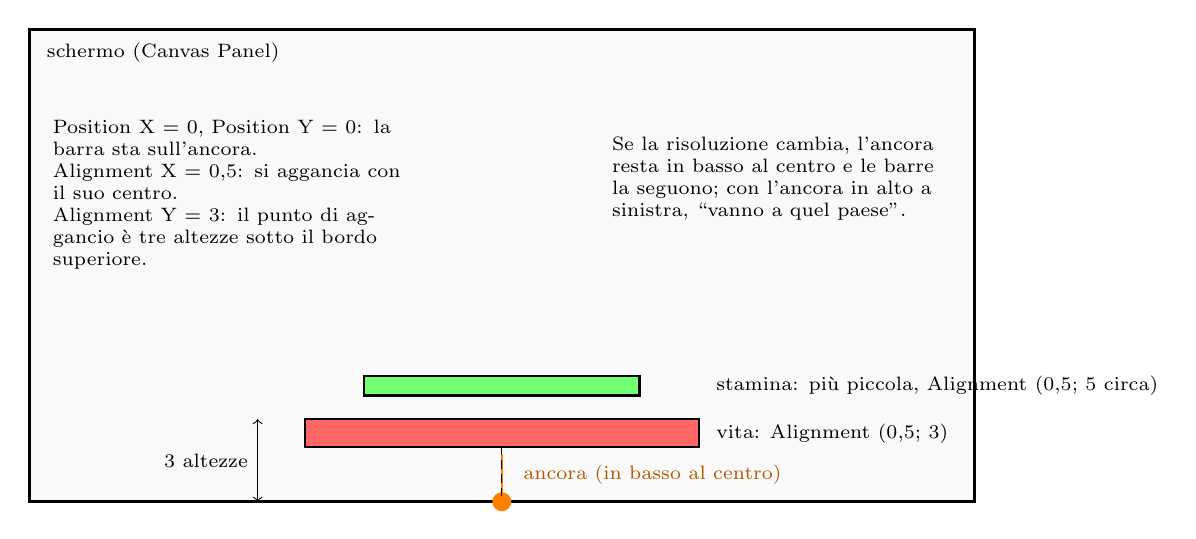
\begin{tikzpicture}[font=\footnotesize, x=1cm, y=1cm]
  % schermo
  \draw[very thick, fill=gray!5] (0,0) rectangle (12,6.0);
  \node[anchor=north west, font=\scriptsize] at (0.1,5.95) {schermo (Canvas Panel)};
  % ancora in basso al centro
  \fill[orange] (6,0) circle (0.12);
  \draw[orange, thick] (6,0) -- (6,0.6);
  \node[orange!70!black, font=\scriptsize, anchor=west] at (6.15,0.35) {ancora (in basso
    al centro)};
  % barra vita: alignment 0.5, 3 -> altezza 0.35 -> bordo superiore a 3*0.35=1.05
  \draw[thick, fill=red!60] (3.5,0.70) rectangle (8.5,1.05);
  \node[font=\scriptsize, anchor=west] at (8.6,0.87) {vita: Alignment (0,5; 3)};
  % barra stamina: posizione indicativa
  \draw[thick, fill=green!55] (4.25,1.35) rectangle (7.75,1.6);
  \node[font=\scriptsize, anchor=west] at (8.6,1.48) {stamina: più piccola, Alignment
    (0,5; 5 circa)};
  % pivot
  \draw[densely dashed] (6,0.70) -- (6,0);
  \draw[<->, thin] (2.9,0) -- node[left, font=\scriptsize]{3 altezze} (2.9,1.05);
  \node[font=\scriptsize, text width=4.6cm, align=left] at (2.6,3.9) {Position X = 0, Position
    Y = 0: la barra sta sull'ancora.\\ Alignment X = 0,5: si aggancia con il suo centro.\\
    Alignment Y = 3: il punto di aggancio è tre altezze sotto il bordo superiore.};
  \node[font=\scriptsize, text width=4.4cm, align=left] at (9.6,4.1) {Se la risoluzione
    cambia, l'ancora resta in basso al centro e le barre la seguono; con l'ancora in alto
    a sinistra, ``vanno a quel paese''.};
\end{tikzpicture}
\caption{Ancore, posizione e allineamento di un widget nel Canvas Panel. La posizione si
misura dall'ancora, l'allineamento sposta il punto dell'elemento che si aggancia
all'ancora, in frazioni della sua dimensione. Schema ricostruito; proporzioni indicative.}
\label{ue11:fig:ancore}
\end{figure}

\paragraph{Approfondimento: ancore e Percent nel libro.} Romero e Sewell (capitolo 7):
``poiché le dimensioni e i rapporti degli schermi possono variare, vogliamo assicurarci
che gli elementi della UI restino nella stessa posizione relativa sullo schermo. Le ancore
servono a definire la posizione desiderata di un widget sul canvas, indipendentemente
dalla dimensione dello schermo.'' Il simbolo a forma di fiore che si vede nel Designer si
chiama \emph{Anchor Medallion}, ``e rappresenta la posizione dell'ancora dell'elemento
selezionato''; la seconda edizione aggiunge che si può anche trascinare direttamente il
fiore nel punto voluto, o espandere \emph{Anchors} per i controlli di precisione. Uno dei
quesiti di fine capitolo chiede se ``i valori X e Y della posizione di un elemento in un
canvas sono sempre relativi all'angolo in alto a sinistra dello schermo'': la risposta è
no, sono relativi all'ancora, che è esattamente ciò che Guido ha scoperto. Sul Percent:
``l'intervallo dei valori va da 0,0 (vuota) a 1,0 (piena)''. Il libro anticipa anche il
motivo per cui serve una divisione: le sue variabili di vita e stamina hanno valore di
default 1,0 proprio perché ``questo valore è usato dai UI meters, che mostrano il grado di
riempimento fra 0,0 e 1,0''. La lezione invece tiene la vita in punti (10) e la stamina in
centesimi (100), e converte al momento di disegnare.

% ---------------------------------------------------------------------
\section{L'HUD sullo schermo: Initialize, Create Widget e Add to Viewport}
\label{ue11:sec:viewport}

\paragraph{L'evento d'inizializzazione.} Nel \textbf{Graph} del widget (``in alto a
destra, Designer e Graph: se clicchi su Graph vai direttamente là''), si tolgono gli eventi
predefiniti e si crea un \textbf{Custom Event}: \textbf{InitializeHealthBar}. Gli serve un
input, ``la referenza stessa al player'': nei Details dell'evento, sotto \emph{Inputs}, il
più, nome \textbf{PlayerRef}, tipo la classe del proprio personaggio (``io ho BP\_Bot2,
ma deve essere il nome del vostro character''), \textbf{Object Reference}: ``quella
azzurra, deve essere azzurra''. A che serve? ``Chiamerà l'Event Dispatcher'': il personaggio
dirà ``ehi, fammi esistere questa UI, mettimela sullo schermo'', e a quel punto bisogna
``bindare l'evento al fatto di inizializzare la barra, quindi dargli subito il valore di
quant'è la vita''. (A chi chiede ``com'è che sotto c'è la freccia bianca?'': è l'evento con
il suo input, che si aggiunge dai Details.)

\paragraph{Il Begin Play del personaggio.} ``Innanzitutto, buona regola, dobbiamo passargli
la PlayerRef.'' In BP\_Bot2, all'\textbf{Event BeginPlay}: ``quando il gioco inizia,
vogliamo che l'HUD, quindi questa schermata, la sua Progress Bar e tutto quanto, vada a
esistere nel mondo, nella nostra viewport''.
\begin{enumerate}
  \item \textbf{Create Widget} (``scusate, non \emph{Add}: è Create Widget''). Il pin
        \textbf{Class} chiede ``la tipologia di asset che andiamo a creare'': WB\_HUD;
  \item il \textbf{Return Value} si promuove a variabile, \textbf{AsHUD}: ``non lo useremo,
        però è una buona cosa sempre fare una referenza, perché magari volete comunicare
        altre volte con il nostro HUD e cambiargli dei valori'';
  \item ``questo lo crea, ma non lo mette nella viewport'': serve \textbf{Add to Viewport},
        con l'HUD come target. In Play, ``ecco a voi che la nostra barra rossa è apparsa
        a schermo'';
  \item infine, dalla variabile AsHUD, la chiamata a \textbf{InitializeHealthBar}, con
        \textbf{PlayerRef} collegato a un \textbf{Get a Reference to Self} (``fate
        \emph{self}, vi appare Get a Reference to Self''). ``Abbiamo detto: ehi, aggiungi
        questo widget alla viewport e inizializza.''
\end{enumerate}
(Durante questa parte il docente ha qualche problema di connessione: ``scusa, ho visto
adesso la chat; sto avendo problemi, devo fare un po' di manutenzione''.)

% ---------------------------------------------------------------------
\section{Il collegamento: Bind Event e Set Percent}
\label{ue11:sec:bind}

\paragraph{Il Bind.} ``Ci manca ovviamente la funzione collegata'': bisogna fare in modo
che l'inizializzazione \emph{agganci} l'aggiornamento della barra all'aggiornamento della
vita. Nel Graph del widget, dopo InitializeHealthBar, dal pin PlayerRef: \textbf{Bind
Event to E\_UpdateHealth} (la trascrizione sente ``bind e update''). Compilando dà errore,
``giustamente'': ``mi serve un evento: che evento devo collegare al fatto che io aggiorno la
mia variabile Health?''. L'evento si crea così: dal pin rosso \textbf{Event} del Bind si
trascina un filo e si sceglie \textbf{Add Custom Event}. ``Mi raccomando: non fate un
Custom Event esterno, tirate fuori proprio da Event e fate Custom Event, perché vi tira
fuori e si porta dietro i due valori che gli abbiamo dato di input, cioè CurrentHealth e
MaxHealth.'' Il nome: \textbf{UpdateHealthBar}.

\paragraph{Che cosa succede.} Una studentessa riassume: ``quindi quando viene
inizializzato, in automatico fa anche Update Health?''. ``Esatto.'' Quando il gioco
inizia, l'HUD ``binda l'evento di aggiornare la barra al nostro Update Health, cioè al
valore numerico che si aggiorna''. ``Creiamo il collegamento'': da quel momento, ``quando si
aggiorna effettivamente il nostro numero, la nostra variabile, allora avviene anche
l'update della barra''.

\paragraph{L'evento senza posti.} ``A me il Bind Event non me l'ha dato'': la studentessa
aveva creato prima, per sbaglio, un Custom Event separato e l'aveva collegato al Bind;
cancellato quello, il Bind risultava ``ancora delegato''. ``Elimina quello che hai
adesso; tira fuori da Event, Custom Event.'' La spiegazione: un Custom Event creato a mano
``non ti dà quei valori di input, CurrentHealth e MaxHealth''; ``questo qua deve essere
creato tramite il collegamento, perché noi gli abbiamo messo degli input''. ``Non deve
essere vuoto: si deve portare dietro i posti per la CurrentHealth e la MaxHealth.
Ricordiamoci il camion.''

\paragraph{Rinominare la barra.} ``Per ordine'': nel Designer, nella \textbf{Hierarchy}
(``ci permette di avere tutte le nostre cosine che abbiamo messo nella UI, tutte belle
elencate''), si seleziona la Progress Bar e con \textbf{F2} la si rinomina
\textbf{ProgressBar\_Health}.

\paragraph{Set Percent.} Nel Graph, la variabile ProgressBar\_Health si trascina
nell'evento UpdateHealthBar e da lei si tira fuori \textbf{Set Percent}. ``In questo caso
però si tratta di una percentuale, quindi è un valore da 0 a 1'': il valore è
\textbf{CurrentHealth diviso MaxHealth}, i due pin dell'evento in un \textbf{Divide}. In
Play, ``la mia barra diminuisce sempre di più, e boom, eccoci qua''
(figure~\ref{ue11:fig:hudgraph} e~\ref{ue11:fig:catena}).

\begin{figure}[htbp]
\centering
\begin{tikzpicture}[font=\scriptsize,
  ue11node/.style={draw, thick, rounded corners=4pt, align=center, fill=gray!8,
                  minimum height=0.9cm, text width=2.0cm},
  ue11ev/.style={ue11node, fill=red!12},
  ue11var/.style={ue11node, fill=blue!10, rounded corners=8pt},
  ue11exec/.style={-{Stealth[length=2.5mm]}, very thick, black!80},
  ue11data/.style={-{Stealth[length=2mm]}, thick, blue!60!black}]
  \node[font=\scriptsize\bfseries, anchor=west] at (-1.0,1.0) {BP\_Bot2, Event Graph};
  \node[ue11ev, text width=1.5cm] (bp) at (0,0) {\textbf{Event BeginPlay}};
  \node[ue11node, text width=1.7cm] (cw) at (2.4,0) {\textbf{Create Widget}\\Class:
    WB\_HUD};
  \node[ue11var, text width=1.4cm] (sh) at (4.7,0) {\textbf{Set}\\AsHUD};
  \node[ue11node, text width=1.6cm] (av) at (6.9,0) {\textbf{Add to Viewport}};
  \node[ue11node, fill=yellow!20, text width=2.5cm] (ih) at (9.7,0)
    {\textbf{Initialize\-Health\-Bar}\\PlayerRef: Self};
  \node[ue11node, fill=yellow!20, text width=2.5cm] (is) at (13.0,0)
    {\textbf{Initialize\-Stamina\-Bar}\\PlayerRef: Self (più tardi)};
  \draw[ue11exec] (bp) -- (cw); \draw[ue11exec] (cw) -- (sh);
  \draw[ue11exec] (sh) -- (av); \draw[ue11exec] (av) -- (ih);
  \draw[ue11exec, dashed] (ih) -- (is);
  \node[font=\scriptsize\bfseries, anchor=west] at (-1.0,-1.6) {WB\_HUD, Graph};
  \node[ue11ev, text width=2.5cm] (ini) at (0.3,-2.7) {\textbf{Initialize\-Health\-Bar}\\
    Custom Event, input PlayerRef};
  \node[ue11node, text width=2.5cm] (bind) at (3.9,-2.7) {\textbf{Bind Event to
    E\_UpdateHealth}\\Target: PlayerRef};
  \node[ue11ev, text width=2.5cm] (upd) at (8.3,-2.7) {\textbf{Update\-Health\-Bar}\\
    CurrentHealth, MaxHealth};
  \node[ue11node, text width=1.6cm] (div) at (10.9,-4.4) {\textbf{Divide}\\Current /
    Max};
  \node[ue11node, text width=2.6cm] (sp) at (12.4,-2.7) {\textbf{Set Percent}\\Target:
    ProgressBar\_Health};
  \draw[ue11exec] (ini) -- (bind);
  \draw[ue11data, red!60!black] (bind) -- node[below]{Event} (upd);
  \draw[ue11exec] (upd) -- (sp);
  \draw[ue11data] (upd.south) |- (div.west);
  \draw[ue11data] (div.north) -- node[right]{In Percent} (sp.south -| div.north);
\end{tikzpicture}
\caption{I due lati dell'HUD. In alto, il personaggio crea il widget, se lo salva, lo
aggiunge alla viewport e gli passa una referenza a se stesso. In basso, il widget usa
quella referenza per legare il proprio evento UpdateHealthBar all'Event Dispatcher del
personaggio: da lì in poi, ogni Call E\_UpdateHealth esegue Set Percent. La chiamata
tratteggiata si aggiunge con la stamina. Schema ricostruito.}
\label{ue11:fig:hudgraph}
\end{figure}

\begin{figure}[htbp]
\centering
\begin{tikzpicture}[font=\footnotesize,
  ue11node/.style={draw, thick, rounded corners=4pt, align=center, fill=gray!8,
                  minimum height=1.0cm, text width=2.5cm},
  ue11exec/.style={-{Stealth[length=2.5mm]}, very thick, black!80}]
  \node[ue11node, fill=orange!15] (pr) at (0,0) {\textbf{BP\_Projectile}\\{\scriptsize
    Sphere Trace, Break Hit Result}};
  \node[ue11node, fill=orange!15] (ad) at (3.4,0) {\textbf{Apply Damage}\\{\scriptsize
    Hit Actor, Base Damage 1}};
  \node[ue11node, fill=red!12] (any) at (6.8,0) {\textbf{Event Any\-Damage}\\{\scriptsize
    in BP\_Bot2}};
  \node[ue11node, fill=blue!10] (hp) at (10.2,0) {\textbf{CurrentHealth}\\{\scriptsize
    Subtract, Clamp, Set}};
  \node[ue11node, fill=yellow!20] (call) at (10.2,-2.2) {\textbf{Call
    E\_UpdateHealth}};
  \node[ue11node, fill=green!10] (ev) at (6.8,-2.2) {\textbf{Update\-Health\-Bar}\\
    {\scriptsize in WB\_HUD (legato)}};
  \node[ue11node, fill=green!10] (pb) at (3.4,-2.2) {\textbf{Set Percent}\\{\scriptsize
    Current / Max}};
  \node[ue11node, fill=green!20] (bar) at (0,-2.2) {\textbf{barra rossa}\\{\scriptsize
    sullo schermo}};
  \draw[ue11exec] (pr) -- (ad); \draw[ue11exec] (ad) -- (any);
  \draw[ue11exec] (any) -- (hp); \draw[ue11exec] (hp) -- (call);
  \draw[ue11exec] (call) -- (ev); \draw[ue11exec] (ev) -- (pb);
  \draw[ue11exec] (pb) -- (bar);
  \node[font=\scriptsize, text width=13cm, align=center] at (5.1,-3.6) {Il proiettile non
    sa nulla della UI, e la UI non sa nulla del proiettile: ognuno parla solo con il
    personaggio.};
\end{tikzpicture}
\caption{Il percorso completo di un colpo, dal proiettile alla barra. Il sistema di danno
di Unreal collega il proiettile al personaggio; l'Event Dispatcher collega il personaggio
all'HUD. Schema riassuntivo.}
\label{ue11:fig:catena}
\end{figure}

\paragraph{I problemi dei presenti.} ``Ci siete, ragazzi?'' Tre casi.
\begin{itemize}
  \item \textbf{Set Percent introvabile.} ``Non mi dà il Set Percent'', e nemmeno i
        Details per cercarlo. Primo controllo: nel Designer, la Progress Bar deve avere la
        spunta \textbf{Is Variable}, altrimenti nel Graph non esiste come variabile. I
        Details mancanti si riaprono da \textbf{Window}, \textbf{Details}. La spunta c'era;
        il vero errore è un altro: lo studente cercava Set Percent trascinando da un altro
        nodo. ``Ah, ok, lo facevo da qua'': Set Percent si trova solo \emph{tirando fuori
        dalla variabile} ProgressBar\_Health, che va presa dalla sezione \emph{Variables}
        (``se non ce l'hai, c'è la tendina'') e trascinata nel grafo. Per la divisione:
        ``tiri fuori dalla CurrentHealth e fai lo slash'', oppure si scrive
        \emph{divide}; poi ``questo diviso per quell'altro''.
  \item \textbf{La torretta che non spara}, a un'altra studentessa: rimandata alla pausa.
  \item \textbf{La barra che non scende.} ``La vita la perdo, perché poi respawno; tuttavia
        graficamente non scende la barra.'' Il Bind c'è, il danno è 1 (``l'ho messo come
        variabile''), la vita è 10. Un Print String dopo il Set Percent, ``attaccalo a In
        String'' (``collega quello verde a quello rosa''), non stampa niente. Allora
        \textbf{F9} sull'evento UpdateHealthBar: ``dice: sta facendo questo evento?''. Il
        breakpoint non scatta. In BP\_Bot2 si scopre perché: nel Begin Play mancava la
        chiamata a \textbf{InitializeHealthBar} dopo Add to Viewport. ``Non stai dicendo al
        gioco che, quando inizia, se io ho dato la vita, mi aggiorni pure la barra.'' Si
        aggiunge da AsHUD, con Self nel PlayerRef; si toglie il breakpoint (``se no te lo
        farà ogni volta''). ``Perfetto, grazie.''
\end{itemize}

\paragraph{Il portatile surriscaldato.} Un altro studente non riesce a seguire: ``sta
andando a scatti'', ``è troppo surriscaldato il computer''. Il consiglio, per tutti: ``per
chi ha un portatile, prendetevi quelle basette con le ventole'': ``col portatile quello
diventa un vulcano a un certo punto''. Lo studente ce l'ha già: ``ah, ok. Quindi sta proprio
andando pesantissimo''. ``Lascialo riposare il nostro soldato, tranquillo: tanto poi c'è la
registrazione.''

\paragraph{Approfondimento: Bind Event contro i Binding del libro.} Qui la lezione e il
libro scelgono due strade diverse, e vale la pena capire perché. Romero e Sewell
(capitolo 7) usano i \textbf{Binding} delle proprietà: accanto al campo \emph{Percent}
della Progress Bar c'è un pulsante \emph{Bind}; scegliendo \emph{Create Binding}, l'editor
crea una funzione che restituisce il valore, in cui gli autori mettono \emph{Get Player
Character}, \emph{Cast To FirstPersonCharacter} e il Get della vita. ``I Binding ci danno
la possibilità di legare variabili o funzioni di un Blueprint a un Widget. Ogni volta che
la variabile o la funzione è aggiornata, il cambiamento si riflette automaticamente nel
Widget.'' Il prezzo, per il funzionamento generale di UMG, è che una funzione di Binding
viene valutata \emph{a ogni frame}, che il valore sia cambiato o no (e, nell'esempio del
libro, con un cast a ogni valutazione). Lo schema della lezione è \emph{a eventi}: la barra
si aggiorna solo quando il personaggio chiama E\_UpdateHealth, cioè quando la vita cambia
davvero. Per due barre la differenza di prestazioni è trascurabile; diventa importante
negli HUD con molti elementi, e soprattutto rende esplicito \emph{chi} aggiorna \emph{che
cosa}. Sul Bind Event, invece, il libro (capitolo 4) dice la stessa cosa del docente:
``c'è un nodo Bind Event che lega un evento a un altro evento o a un Event Dispatcher, che
può stare in un altro Blueprint. Quando un evento è chiamato, tutti gli altri eventi legati
a lui sono chiamati'', e il Custom Event si crea trascinando ``dal pin rosso del nodo Bind
Event'' e scegliendo \emph{Add Custom Event}. Un dettaglio generale: un Custom Event creato
dal pin riceve automaticamente la \emph{firma} del dispatcher (i suoi input); se in seguito
si aggiungono input al dispatcher, gli eventi legati vanno aggiornati, e l'editor lo segnala
con un errore di firma alla compilazione.

% ---------------------------------------------------------------------
\section{La seconda barra e la corsa}
\label{ue11:sec:corsa}

``Abbiamo un quarto d'oretta. Sai che facciamo? Andiamo a creare la nostra barra della
stamina e facciamo insieme la stamina, così dopo magari facciamo qualcos'altro, che è il
menu in questo caso.''

\paragraph{La barra copiata.} ``Più che metterne una nuova'', nel Designer di WB\_HUD si
copia la barra della vita con \textbf{Ctrl+C} e \textbf{Ctrl+V}. La copia ha ancora
l'ancora in basso al centro; si azzerano le posizioni, \textbf{Alignment} X a \textbf{0,5}
e Y più alto, perché stia sopra la barra rossa (il docente dice ``non 3, ma la mettiamo
tipo a 2, e facciamo 5'', poi ``facciamo 5''), la si fa ``un pochino più piccola'' (con i
campi della dimensione, ``1,8, ma sì, 2'': ``questi rettangolini servono per essere un po'
più precisi''), e verde. ``Se volete, ragazzi, sbizzarritevi: i colori, proprio pastelli in
mano, fate come volete.''

\paragraph{InitializeStaminaBar.} ``Facciamo la stessa identica cosa per l'inizializzazione
della barra'': nel Graph, un altro Custom Event, \textbf{InitializeStaminaBar}, con lo
stesso input \textbf{PlayerRef} (``fortunatamente, se avete già fatto l'input, vi dice già:
ce l'ho, PlayerRef''). ``Per adesso lo lasciamo così, perché dobbiamo creare un altro
Event Dispatcher, che sarà invece l'update della stamina.''

\paragraph{IA\_Run.} Torniamo nel bot: ``dobbiamo far correre il nostro player''. Serve
un'\textbf{Input Action} nuova, \textbf{IA\_Run}, accanto a IA\_Look, IA\_Move e IA\_Jump;
la si era fatta la volta scorsa per il cavaliere, e ``fortunatamente'' basta una volta:
``questa è la bellezza del context: la mappatura degli input è separata dal player'', e
``la posso passare da player a player''. Per chi non ce l'ha:
\begin{enumerate}
  \item da un'azione qualsiasi, tasto destro, \textbf{Show in Folder View}; si
        \textbf{duplica} IA\_Jump e la si chiama IA\_Run. ``Se non sbaglio, Jump e Run
        sono uguali'': entrambe hanno un valore booleano (\emph{Digital});
  \item nell'\textbf{IMC} (\emph{Input Mapping Context}), il più, IA\_Run, e nella
        tendina la \textbf{tastiera}: ``cliccate sulla tastiera, premete Shift'', ``in modo
        da dire: guarda che questo è l'input collegato alla corsa''.
\end{enumerate}
``Io l'ho spiegato molto velocemente, perché so che, se qualcuno nel caso non avesse
visto, poi mi dica.''

\paragraph{Gli stati dell'evento.} Nel bot, l'evento \textbf{IA\_Run} mostra le sue uscite
(\emph{Triggered}, \emph{Started}, \emph{Ongoing}, \emph{Canceled}, \emph{Completed});
``in questo caso ci interesseranno solamente lo \textbf{Started} e il
\textbf{Completed}'': l'inizio e la fine della pressione.

\paragraph{Camminare di default.} ``Per dire già che il player deve camminare di default'',
si guarda il Blend Space del bot: la camminata è a 250, ``facciamo 300, un po' più alto''.
Nel \textbf{Character Movement}, categoria \emph{Character Movement: Walking},
\textbf{Max Walk Speed} a \textbf{300}: ``da adesso in poi il nostro character camminerà''.
(Se i passi non suonano, ``lo fixiamo poi'': il docente aveva aggiunto i suoni dei passi
anche all'animazione di camminata prima della lezione, ``perché prima solamente
correvamo''.)

\paragraph{Correre.} Due \textbf{Set Max Walk Speed}, entrambi con il Character Movement
come target (``ricordatevi di tutti e due di collegarli''): uno allo \textbf{Started}, a
\textbf{500}, uno al \textbf{Completed}, a \textbf{300}. (Il docente dice prima 600, poi
``500 era? Facciamo 500, va bene'', il valore massimo del Blend Space.) In Play: ``cammino;
Shift, corro; Shift, lascio''. ``Sicuramente possiamo mettere un po' di smooth
all'animazione'', con un \emph{blend in} e un \emph{blend out}: ``questo è un fix che
possiamo fare dopo, tranquillamente''.

\paragraph{La stamina di Dark Souls.} ``Qualcuno di voi ha in mente Dark Souls? La stamina
di Dark Souls, o in generale, molto spesso la stamina funziona in questo modo'': ``viene
persa durante un quantitativo di tempo, se si fa una certa azione, in questo caso correre:
viene levata gradualmente'', e quando l'azione smette ritorna su piano piano. ``Visto che
parliamo di tempo, useremo due \textbf{timer}'', come per la torretta, ``per far sì che
queste due cose vadano a scalare nel tempo''. Mancano cinque minuti alla pausa: ``facciamo
adesso un piccolo timer, oppure vogliamo andare già in pausa?''. Si va in pausa: ``la
prova è 25'', ``facciamo 17 e 55 e ci rivediamo''.

\paragraph{Approfondimento: lo sprint nel libro.} Romero e Sewell costruiscono lo sprint nel
capitolo 6 con il sistema di input precedente (l'\emph{Action Mapping} ``Sprint'' sul
tasto Shift sinistro, gli eventi \emph{Pressed} e \emph{Released}) e due \emph{Set Max
Walk Speed}, esattamente come la lezione con l'Enhanced Input (Started e Completed). Nel
capitolo 8 fanno un'osservazione di design che spiega perché la stamina serve: senza un
vincolo, ``non ci sarebbe niente a scoraggiare il giocatore dal tenere sempre premuto
Shift mentre si muove''; ``se un'opzione è così attraente che il giocatore si sente
costretto a usarla sempre, allora non aumenta il numero di scelte interessanti''. ``Dal
punto di vista del giocatore, il risultato sarebbe lo stesso se aumentassimo semplicemente
la velocità di base fino a quella dello sprint.'' La stamina trasforma lo sprint in una
\emph{risorsa}: correre ora significa non poter correre fra poco. È la stessa logica della
stamina di Dark Souls, dove la stessa barra è condivisa da corsa, schivata, parata e
attacco, e ogni scelta ha un costo.

% ---------------------------------------------------------------------
\section{La pausa: le torrette e i bot degli studenti}
\label{ue11:sec:pausa}

La pausa, come spesso in questo corso, diventa uno sportello di correzioni. Il docente
resta collegato e guarda i progetti uno alla volta, in condivisione di schermo
(``quando condividi, fai \emph{condividi schermo}, non condividere Unreal, perché è più
facile: stiamo schermando più grande'').

\paragraph{Lo Shift che non corre.} Il primo studente: ``se mi muovo normalmente cammina,
se premo Shift non corre''. ``Allora c'hai qualche cosa che non va nell'IA\_Run.'' La cosa
resta in sospeso: il problema dello stesso tipo tornerà, più grave, alla fine della lezione
(sezione~\ref{ue11:sec:barrastamina}).

\subsection{La torretta di Tommaso}

``Io entro, mi vede, ma non spara.'' Il tag Player c'è.
\begin{enumerate}
  \item \textbf{La collisione della mesh del bot}: ``non l'avevo messa''. Mesh, Collision,
        Custom, Detection Turret in Block (e Projectile Trace: ``va benissimo''). Ora la
        torretta lo segue, ma non spara.
  \item \textbf{Il Trace Channel}: nella torretta, il trace di rilevamento usava il canale
        sbagliato. ``Cambia Trace Channel'' a \textbf{Detection Turret} (``no, no, torna
        indietro; Ctrl+Z''). ``Ok, benissimo.''
  \item \textbf{La funzione dello spawn}: alla torretta di Tommaso manca proprio la
        funzione che fa nascere il proiettile. Il docente gliela passa con ``un
        trucchettino'': ``la cosa bella dei Blueprint è che puoi incollarli in un file di
        testo, copiarli tutti quanti''. Seleziona i nodi della sua funzione, Ctrl+C, li
        incolla in un file \emph{.txt} (``Fix, funzione Spawn'') e glielo manda su
        Discord, in privato. Tommaso scarica il file, ne copia tutto il testo e lo incolla
        con Ctrl+V nel grafo di Unreal: i nodi ricompaiono.
  \item \textbf{Sistemare l'incollato}: ``adesso c'hai degli errori, eh? Perché devi
        sistemarlo''; ``prima fix, poi ordina''. La funzione si rinomina con F2
        \textbf{Spawn Projectile}. Servono i due punti di uscita: nei Components, Add,
        due \textbf{Scene Component}, \textbf{ProjectileSpawn1} e \textbf{ProjectileSpawn2}
        (copiati con Ctrl+C e Ctrl+V), agganciati al \textbf{cannone} della torretta e
        spostati ``ai bocchettoni della mesh'', ``poco fuori la canna''.
  \item \textbf{Lo Spawn Actor rifatto}: il nodo incollato dà un errore sull'\emph{Spawn
        Actor} (``non ti spawno nessun actor''); l'errore sull'\emph{Instigator} invece
        ``va bene, non ci interessa''. ``Facciamo prima'': si cancella e si rifà
        \textbf{Spawn Actor from Class}; tasto destro sullo \emph{Spawn Transform},
        \textbf{Split Struct Pin}; si collegano Location e Rotation dei due Scene; la
        \textbf{Class} è il proiettile, BP\_Projectile.
  \item Una curiosità di Tommaso, nel frattempo: ``pure la barra della stamina, io gli ho
        dato un colore, ma me la dà grigia''. ``Forse è vuota'': il \emph{Percent} è a 0,
        e una Progress Bar vuota mostra solo lo sfondo. ``Faccio 1.''
  \item \textbf{Chiamare la funzione}: la torretta ancora non spara, ``perché non
        spawni'': nello \emph{Shoot}, al posto delle due vecchie chiamate, va chiamata la
        nuova \textbf{Spawn Projectile}.
  \item \textbf{Le collisioni della torretta}: il proiettile non deve fermarsi sulla
        torretta stessa. Sul cannone, sulla sfera di rilevamento e sul pivot, il canale
        Projectile Trace va su \textbf{Ignore} (``devi ignorare tutto, anche il pivot'').
\end{enumerate}
La torretta di Tommaso ancora non spara; ``aspetta, adesso facciamo fare Lucrezia, che è
un po' che aspetta''. Si riprenderà dopo la pausa.

\subsection{Il bot di Lucrezia, risolto}

\paragraph{Il Validated Get sulla variabile sbagliata.} Con Shift il bot di Lucrezia ora
``va più veloce'': ``quello almeno va benissimo''; quindi il personaggio si muove, ``è un
problema di animazioni''. Il docente esclude un doppio scheletro (``non vorrei che avessi
un doppio scheletro e te l'avessi fatto su un altro'': ne ha uno solo), poi mette un
Print String sull'uscita \textbf{Is Not Valid} del Validated Get, all'inizio dell'Update.
Stampa: ``ecco il nostro problema: la referenza a questo actor non è valida''. Il motivo:
``hai messo nel Validated Get la variabile del PB\_Bot, non del BP\_Bot, che sono due
diverse'': nell'Animation Blueprint c'erano due variabili quasi omonime, e il Validated
Get controllava quella che l'Initialize non riempiva mai. Si cancella, si prende la
variabile giusta (\textbf{AsBP\_Bot}), tasto destro, \textbf{Convert to Validated Get}, si
ricollega. ``Dovremmo aver scoperto l'arcano.'' ``Era lui.''

\paragraph{La regola di ritorno all'Idle.} Ora il bot anima, ma ``continua a camminare sul
posto'' quando si ferma. Nella State Machine, la regola Walk $\rightarrow$ Idle era
\emph{GroundSpeed $<$ 0}: ``attenzione, non è minore, è \textbf{minore o uguale}'',
perché una velocità negativa non esiste (la lunghezza di un vettore è sempre $\ge 0$), e con
il minore stretto la regola non è mai vera (``solo se sarà meno uno la velocità'').

\paragraph{Il Lean, di nuovo.} Correndo e girando, il bot ``non si inclina tantissimo'':
la stessa correzione fatta a inizio lezione (``come abbiamo fatto anche con Tommaso'': la
trascrizione attribuisce qui a Tommaso il Lean corretto all'inizio). Nel Blend Space i
campioni da $\pm 10$ a $\pm 1$, poi l'asse, nelle \emph{Axis Settings} dei Details, da $-1$
a 1. ``Ecco che si piega leggermente.''

\paragraph{La torretta di Lucrezia.} Poi la torretta, aperta con \emph{Edit BP\_Turret} dal
livello (``lo fai diretto''). ``Questo è un po' incasinato, eh? Vabbè, tranquillo.'' In
ordine:
\begin{itemize}
  \item \textbf{Begin Overlap}: il fix di inizio lezione, Get Player Pawn al posto
        dell'Other Actor nel Set di PlayerTarget;
  \item \textbf{Move Turret} (la rotazione verso il bersaglio): il nodo di rotazione
        usato era un altro, e si sostituisce con \textbf{Find Relative Look at
        Rotation}, che vuole uno \emph{Start Transform} (``non ti serve il Get Actor
        Rotation, ma devi invocare il \textbf{Get Actor Transform}'', ``pinnetto
        arancione per pinnetto arancione'') e una \emph{Target Location}, il \textbf{Get
        Actor Location} del PlayerTarget. Del risultato, con \emph{Split Struct Pin}, si
        usa la \textbf{Z} (lo Yaw) come \emph{Target} dell'interpolazione; un vecchio
        ``meno'' non serve più; nel \emph{Delta Time} va \textbf{Get World Delta Seconds}.
        La trascrizione, qui, è troppo frammentaria per ricostruire il grafo nodo per nodo;
        il senso è quello della rotazione della torretta costruita nelle lezioni
        precedenti;
  \item \textbf{Shoot}: Branch, Sequence, i due \emph{Do Once} con lo Spawn Projectile e il
        Delay, il \emph{Fire Rate}: ``va benissimo'';
  \item un secondo \emph{On Component Begin Overlap} rimasto da una prova (``probabilmente
        una cosa che avevo cancellato'', ``l'avevo spostata''): si elimina; l'\emph{End
        Overlap} e il Tick si tengono;
  \item \textbf{il tag}: la torretta ancora non la segue. Il tag Player era stato messo nei
        \emph{Component Tags} della mesh: ``attenzione, non della mesh, ma quello sotto'':
        i \textbf{Tags} dell'\emph{actor}, e con la stessa maiuscola.
\end{itemize}

\paragraph{Il proiettile assassino.} Ora la torretta spara (``sei un po' alta''), ma
emergono tre problemi del proiettile, uno dopo l'altro.
\begin{enumerate}
  \item I proiettili urtano la camera del personaggio: sulla \emph{Sphere} del proiettile,
        Collision, \textbf{Camera} su \textbf{Ignore}.
  \item I proiettili ``non si distruggono se il character gli va addosso'': la Sphere
        Trace aveva \textbf{Radius 0}, ``quindi è grande niente''. A \textbf{20}.
  \item Ora un colpo e il bot ``si blocca proprio tutto'', anche se la vita non è finita.
        Nel proiettile, dopo il colpo, c'era un \textbf{Destroy Actor} con l'\emph{Hit
        Actor} come target (un ramo chiamato \emph{Kill Target}): ``se colpisco qualcosa,
        distruggimi quello che ho colpito''. Il proiettile cancellava il personaggio dal
        mondo. Al suo posto: \textbf{Apply Damage} (Hit Actor nel Damaged Actor, Base
        Damage 1), e poi \textbf{Destroy Actor} senza target, cioè \emph{self}: ``quando
        collide con qualcosa, distruggi il proiettile: si autodistrugge''.
\end{enumerate}

\paragraph{La vita a zero e la NewVar.} Ora il bot ``muore praticamente subito'': la
\textbf{MaxHealth} aveva default 0, e il Clamp riduceva a zero qualunque vita. MaxHealth a
10. Poi il contrario: il primo colpo toglie vita, ``poi adesso è immortale''. Nell'Event
AnyDamage c'era un Set su una variabile \textbf{NewVar}, creata per sbaglio, invece che
sulla CurrentHealth: ``stai praticamente mettendo una variabile nuova come vita''. Si
sostituisce con \emph{Set CurrentHealth}, ricollegando il Return Value del Clamp e il
valore al Branch del minore o uguale. ``Perfetto. Grazie mille.''

\paragraph{Approfondimento: i Blueprint come testo.} Il ``trucchettino'' del file di testo
funziona perché Unreal copia i nodi negli appunti in un formato testuale (lo stesso
formato \emph{T3D} usato per copiare gli actor fra livelli): ogni nodo diventa un blocco
\texttt{Begin Object} \dots\ \texttt{End Object} con la sua classe, la posizione nel grafo,
i valori dei pin e i collegamenti. Incollando quel testo in un altro grafo, anche di un
altro progetto, l'editor ricrea i nodi. È il modo più rapido per condividere un pezzo di
logica in chat o su un forum, ed esistono siti che lo visualizzano come immagine. Il
limite è quello visto a lezione: i riferimenti a variabili, componenti e funzioni del
Blueprint d'origine non esistono nel Blueprint di destinazione, e i nodi che li usano
arrivano ``rotti'' e vanno ricollegati o ricreati (come gli Scene Component e lo Spawn
Actor di Tommaso). Questa è una nozione generale dell'editor, non trattata nei due libri.

% ---------------------------------------------------------------------
\section{Dopo la pausa: ancora la torretta, e gli annunci}
\label{ue11:sec:annunci}

``Eccoci qua, ragazzi, siamo ritornati.'' Tommaso ha provato a togliere e rimettere la
torretta: niente.

\paragraph{L'Event Tick che manca.} ``Io credo che sia \emph{not valid} il PlayerTarget,
probabilmente.'' Il Begin Overlap e il timer sono giusti; ``ah, ti manca il Tick''.
Nell'Event Graph della torretta non c'è l'\textbf{Event Tick} che, a ogni frame, controlla
il bersaglio e spara. Si ricrea: Event Tick, \textbf{Is Valid} (``punto interrogativo,
quello sotto'') con il PlayerTarget come oggetto, e sull'uscita \emph{Is Valid} la
funzione \textbf{Shoot}. La torretta spara.

\paragraph{Fire Rate e velocità.} ``È un po' lento a sparare'': il \textbf{Fire Rate}, fra
le variabili della torretta, è a 0,2 (la trascrizione dice ``02''); il docente suggerisce
un altro valore (``facciamolo 0,7''; il suo è 0,5): dalla trascrizione non si capisce se
il valore sia un intervallo fra i colpi o un'altra cosa nel grafo di Tommaso, e il capitolo
non lo ricostruisce. ``Il proiettile è molto lento'': nel proiettile, il componente
\textbf{Projectile Movement}, \textbf{Initial Speed} e \textbf{Max Speed} a \textbf{1000}.

\paragraph{Il danno che non arriva alla barra.} ``Però non prendo danno.'' Il proiettile ha
l'Apply Damage, ``va bene così''; nel BP\_Bot, però, l'\textbf{Add to Viewport} non era
collegato con il pin di esecuzione all'InitializeHealthBar (``vedi che non è stato
attaccato''). E non basta: nell'Event AnyDamage il Set era su \textbf{MaxHealth} invece che
su CurrentHealth (``ha impostato MaxHealth, non CurrentHealth''). Corretti entrambi:
``vediamo se muoio''. ``Ottimo, perfetto: di solito tutto il casino.''

\paragraph{Il calendario.} Prima di riprendere, gli annunci.
\begin{itemize}
  \item Il \textbf{menu}: ``se non ce la facciamo a fare il menu oggi, lo facciamo la
        prossima volta, e tanto la prossima volta sarà l'ultima lezione che avremo''.
  \item Dopo: ``poi avrete Davide, quindi avrete martedì con me e Davide''; ``poi
        inizierete a fare roba di \textbf{level design}''.
  \item Manca ``un piccolo asset da fare'', le \textbf{porte}: ``possiamo farlo
        tranquillamente la prossima volta, o ve lo lascio come compito, perché sono sicuro
        che lo sapete fare''. ``La timeline l'abbiamo già affrontata'' (il compito è
        descritto nella sezione~\ref{ue11:sec:chiusura}).
\end{itemize}
(``Non stai condividendo?'' ``Ah, ok. Grazie mille, Lucrezia.'')

% ---------------------------------------------------------------------
\section{I due timer della stamina}
\label{ue11:sec:timer}

``E adesso incominciamo a fare questo bellissimo scattino.'' Si torna al bot del docente
(``il proiettile non ci serve più; ci serve botolino''). Il movimento c'è già (500 e 300
sull'IA\_Run); ``abbiamo detto che dobbiamo fare due timer ben distinti: uno che la consuma
e uno che la riporta al suo massimo, piano piano nel tempo''.

\subsection{Il timer che consuma}

\paragraph{Set Timer by Event.} Dopo il Set Max Walk Speed a 500 (lo Started), un
\textbf{Set Timer by Event}.
\begin{itemize}
  \item il pin \textbf{Time} si promuove a variabile, \textbf{TimeStamina}, ``in modo tale
        da avere questa variabile molto più controllabile''; default \textbf{0,05}
        (impostato poco dopo: ``piccola cosa, semplicemente non l'abbiamo impostato''):
        ``questo è il tempo in cui verrà eseguito il timer, ogni 0,05 secondi'';
  \item \textbf{Looping} attivo; \textbf{Max Once Per Frame} attivo;
  \item ``il timer, come abbiamo visto le scorse volte, è un evento collegato'': dal pin
        rosso \textbf{Event} si crea un Custom Event, \textbf{StaminaDeduction}.
\end{itemize}

\paragraph{Le variabili.} ``Lo stesso discorso vale come per la Health'': due Float,
\textbf{CurrentStamina} e \textbf{MaxStamina}, entrambe a \textbf{100}.

\paragraph{StaminaDeduction.} Il corpo è quasi identico a quello della vita:
\begin{enumerate}
  \item CurrentStamina \textbf{Subtract} \textbf{1} (``verrà sottratto di 1 ogni 0,05
        secondi'');
  \item \textbf{Clamp (float)}, fra 0 e MaxStamina (``il nostro valore oscillerà fra un
        minimo di 0 e un massimo di MaxStamina, che è 100'');
  \item \textbf{Set CurrentStamina}: ``farà 99, 98, 97\dots''.
\end{enumerate}
``Questo è lo stesso discorso che vale per la Health, è quasi praticamente medesimo.''

\paragraph{Quando fermarsi: OR con Is Falling.} Poi un \textbf{Branch} (``tenete proprio
B'' e cliccate: la scorciatoia del Branch): se la CurrentStamina è \textbf{minore o uguale
a zero}, si fermerà la corsa (``ancora non abbiamo la funzione, ma la lasciamo così''). E
una piccola accortezza nata ``durante il testing'': ``ci sono dei problemi anche nel caso
noi stiamo cadendo''. ``Io tengo premuto il tasto mentre sto cadendo: non voglio che la
stamina venga consumata, perché non stiamo correndo effettivamente.'' Dal Character
Movement, \textbf{Is Falling} (``ce ne sono due: prendete quello \emph{Nav Movement}'',
quello con l'ingresso blu e l'uscita rossa), e i due booleani in un \textbf{OR Boolean}:
``OR è l'operatore che ci permette di dire \emph{o}: ti fermi se sei minore di zero
\emph{o} se stai cadendo'' (figura~\ref{ue11:fig:deduction}).

\paragraph{Il timer che non si ferma.} Con un Print String della CurrentStamina: ``io
cammino, cammino, comincio a sprintare: i valori scendono. Ma se anche smetto di correre,
i valori continuano a scendere, perché non stoppiamo mai il nostro timer.'' La soluzione è
tenere un \emph{riferimento} al timer: il \textbf{Return Value} di Set Timer by Event (un
\emph{Timer Handle}) si promuove a variabile, \textbf{TimerDeductionStamina}, ``in modo tale
che sia più comodo controllarlo da varie parti''. Al \textbf{Completed} dell'IA\_Run, dopo
il Set Max Walk Speed a 300: un Get di TimerDeductionStamina e \textbf{Clear and Invalidate
Timer by Handle}, ``andiamo a invalidare e fermare il nostro timer''. In Play: ``corro,
smetto di correre: si è fermato a 75''.

\subsection{Il timer che ricarica}

\paragraph{Il secondo timer.} ``Altro problema: se io ricomincio a correre, ripartirà da 75,
non torna piano piano verso 100.'' Quando si smette di correre bisogna ``fare l'opposto'':
subito dopo il Clear, un altro \textbf{Set Timer by Event}, ``sempre in Looping, sempre in
Max Once Per Frame''. Per il tempo il docente usa la stessa TimeStamina, ``ma volendo si può
fare a un valore che volete voi: volete che uno si recuperi più veloce oppure più lento,
sta a voi''. Il suo evento è un Custom Event, \textbf{RegainStamina}: ``non c'è neanche
tanto da sbizzarrirci: è letteralmente la copia di questo''. Si copiano i nodi della
deduzione fino al Set e ``l'unica cosa che andiamo a cambiare è che invece di sottrarre
uno, andiamo ad aggiungere uno'': \textbf{Add} 1, Clamp, Set CurrentStamina.

\paragraph{Fermare anche lui.} Stesso schema al contrario: il Return Value si promuove a
\textbf{TimerRegainStamina}, e allo \textbf{Started} (``quando noi ricominciamo a
correre'') un \textbf{Clear and Invalidate Timer by Handle} su di lui. In Play: ``comincio a
correre, i valori cominciano a scendere; lascio, i valori piano piano risalgono fino a
100''.

\paragraph{Fermarsi a 100.} Ma arrivato a 100, il timer della ricarica continua a girare,
inutilmente. In RegainStamina, dopo il Set, un \textbf{Branch}: se la CurrentStamina è
\textbf{maggiore o uguale} alla MaxStamina, un Clear and Invalidate Timer by Handle su
TimerRegainStamina, ``cioè lo stesso timer che stiamo avendo'': ``se arrivi a 100,
smettila''. ``Non stampo più, si è fermato.''

\subsection{L'evento StopRunning}

\paragraph{La corsa che non finisce.} ``C'è una particolarità'': correndo fino a zero, ``il
nostro character non si ferma, e neanche il timer si ferma'', e il personaggio continua a
correre con la stamina vuota. Serve la funzione di \emph{smettere di correre} anche
\emph{dentro} StaminaDeduction, non solo al rilascio del tasto. ``Per comodità, invece di
fare una funzione a parte'': si stacca il \textbf{Completed} dalla sua catena (Set Max Walk
Speed 300, Clear del timer di deduzione, Set Timer della ricarica), e all'inizio della
catena si mette un nuovo Custom Event, \textbf{StopRunning}. Poi:
\begin{itemize}
  \item il \textbf{Completed} chiama StopRunning;
  \item il ramo \textbf{True} del Branch di StaminaDeduction (stamina $\le$ 0 OR Is
        Falling) chiama StopRunning.
\end{itemize}
``Questa cosa ci serve semplicemente per trasportarci il fatto di \emph{fermati}: vai a
300 di velocità e smettila di sottrarmi la stamina, da questo evento che possiamo
trasportare un po' dappertutto.'' In Play: ``corro, corro, corro, arrivo fino a zero, mi
fermo in automatico'', la stamina risale; ``e poi devo semplicemente ripremere per poter
scattare'' (lo \emph{Started} scatta solo alla pressione). ``Abbiamo fatto il nostro
sistema di stamina'' (figura~\ref{ue11:fig:timer}).

\paragraph{Ricapitolare per chi si è perso.} Una studentessa ha perso il pezzo di
RegainStamina; il docente lo ripete: copiare la catena della deduzione, sostituire il meno
con un più, il Branch con il \emph{maggiore o uguale} (``non mi trova il maggiore'': ``io
ho la tastiera più piccola, non ci ho alcuni segni''; ``allora scrivi \emph{greater
equal}''), MaxStamina e CurrentStamina nei due ingressi, sul True il Clear and Invalidate
Timer by Handle con TimerRegainStamina. Poi StopRunning: ``stacchi da qui il Completed, ci
metti un Custom Event al suo posto, e StopRunning ce lo metti anche al Completed''; la
chiamata, ``di colore azzurro'', ``tiri fuori e fai StopRunning'', anche dopo il Branch.
``Ho recuperato tutto.''

\begin{figure}[htbp]
\centering
\begin{tikzpicture}[font=\footnotesize,
  ue11node/.style={draw, thick, rounded corners=4pt, align=center, fill=gray!8,
                  minimum height=0.9cm, text width=2.1cm},
  ue11ev/.style={ue11node, fill=red!12},
  ue11var/.style={ue11node, fill=blue!10, rounded corners=8pt},
  ue11exec/.style={-{Stealth[length=2.5mm]}, very thick, black!80},
  ue11data/.style={-{Stealth[length=2mm]}, thick, blue!60!black}]
  \node[ue11ev, text width=2.3cm] (ev) at (0,0) {\textbf{Stamina\-Deduction}\\{\scriptsize
    ogni 0,05 s}};
  \node[ue11node, text width=1.9cm] (sub) at (2.6,-2.0) {\textbf{Subtract}\\{\scriptsize
    CurrentStamina $-$ 1}};
  \node[ue11node] (cl) at (5.3,-2.0) {\textbf{Clamp (float)}\\{\scriptsize 0 --
    MaxStamina}};
  \node[ue11var] (set) at (3.1,0) {\textbf{Set}\\{\scriptsize CurrentStamina}};
  \node[ue11node, fill=yellow!20, text width=2.6cm] (call) at (6.4,0) {\textbf{Call
    E\_Update\-Stamina}\\{\scriptsize (aggiunta dopo)}};
  \node[ue11node, text width=1.4cm] (br) at (9.3,0) {\textbf{Branch}};
  \node[ue11node, text width=1.5cm] (or) at (9.3,-2.0) {\textbf{OR}};
  \node[ue11node, text width=2.1cm] (le) at (7.4,-3.7) {CurrentStamina $\le$ 0};
  \node[ue11node, text width=2.8cm] (fall) at (10.8,-3.7) {\textbf{Is Falling}\\
    {\scriptsize (Nav Movement, dal Character Movement)}};
  \node[ue11ev, text width=2.0cm] (stop) at (12.2,0) {\textbf{StopRunning}};
  \draw[ue11exec] (ev) -- (set); \draw[ue11exec] (set) -- (call);
  \draw[ue11exec] (call) -- (br);
  \draw[ue11exec] (br) -- node[above, font=\scriptsize]{True} (stop);
  \draw[ue11data] (ev.south) |- (sub.west);
  \draw[ue11data] (sub) -- (cl); \draw[ue11data] (cl.north) |- ([yshift=-3mm]set.east);
  \draw[ue11data] (le.north) -- (or.south west);
  \draw[ue11data] (fall.north) -- (or.south east);
  \draw[ue11data] (or) -- node[right, font=\scriptsize]{Condition} (br);
\end{tikzpicture}
\caption{L'evento del timer che consuma la stamina. Il calcolo è lo stesso della vita, con
1 al posto del danno; la corsa si interrompe se la stamina è finita oppure se il
personaggio sta cadendo. La chiamata dell'Event Dispatcher si inserisce dopo, per la barra.
Ricostruzione dalla lezione.}
\label{ue11:fig:deduction}
\end{figure}

\begin{figure}[htbp]
\centering
\begin{tikzpicture}[font=\footnotesize,
  ue11state/.style={draw, very thick, rounded corners=10pt, align=center,
                    minimum height=1.6cm, text width=3.8cm},
  ue11tr/.style={-{Stealth[length=2.5mm]}, very thick}]
  \node[ue11state, fill=gray!10] (walk) at (0,0) {\textbf{Cammina}\\{\scriptsize Max
    Walk Speed 300}\\{\scriptsize timer RegainStamina attivo, +1 ogni 0,05 s, fino a
    100}};
  \node[ue11state, fill=green!10] (run) at (8.4,0) {\textbf{Corre}\\{\scriptsize Max
    Walk Speed 500}\\{\scriptsize timer StaminaDeduction attivo, $-1$ ogni 0,05 s}};
  \node[ue11state, fill=yellow!15, text width=3.2cm, minimum height=1.1cm] (full) at
    (0,-4.4) {\textbf{Ferma a 100}\\{\scriptsize nessun timer attivo}};
  \draw[ue11tr] ([yshift=4mm]walk.east) -- node[above, font=\scriptsize, text
    width=4.2cm, align=center]{IA\_Run \textbf{Started}: speed 500, Clear
    TimerRegainStamina, Set Timer StaminaDeduction} ([yshift=4mm]run.west);
  \draw[ue11tr] ([yshift=-4mm]run.west) -- node[below, font=\scriptsize, text
    width=4.2cm, align=center]{\textbf{StopRunning}: dal Completed, oppure stamina $\le$
    0 OR Is Falling. Speed 300, Clear TimerDeductionStamina, Set Timer RegainStamina}
    ([yshift=-4mm]walk.east);
  \draw[ue11tr] (walk.south) -- node[left, font=\scriptsize, text width=3.0cm,
    align=right]{CurrentStamina $\ge$ MaxStamina: Clear TimerRegainStamina} (full.north);
  \draw[ue11tr] (full.east) -| node[pos=0.25, below, font=\scriptsize]{IA\_Run Started}
    (run.south);
\end{tikzpicture}
\caption{I due timer della stamina come due stati. Ogni passaggio spegne il timer dello
stato che si lascia (con il suo Timer Handle) e accende quello dello stato in cui si entra.
A stamina finita la corsa si interrompe da sola; per ricominciare bisogna premere di nuovo
Shift. Schema ricostruito.}
\label{ue11:fig:timer}
\end{figure}

\paragraph{Approfondimento: la stamina nel libro.} Romero e Sewell costruiscono la stessa
meccanica nel capitolo 8, \emph{Draining and regenerating stamina}, con scelte diverse che
è utile confrontare.
\begin{itemize}
  \item \textbf{Un timer solo.} Invece di due timer, il libro usa un unico evento,
        \emph{ManageStamina}, chiamato da un timer in loop ogni \emph{Stamina Drain and
        Recharge Time} = 0,2 secondi (``questo timer chiamerà la funzione cinque volte al
        secondo''); dentro, a seconda di un booleano \emph{IsSprinting}, l'evento consuma
        o ricarica. È lo schema dei due stati della figura~\ref{ue11:fig:timer} con un solo
        orologio.
  \item \textbf{Per nome, non per handle.} Il timer è creato con \emph{Set Timer by Function
        Name} e fermato con \emph{Clear Timer by Function Name}; per non sbagliare a
        scrivere il nome, il libro lo salva in una variabile stringa
        (\emph{StaminaManagerName}), ``per evitare bug dovuti a errori di battitura''. Prima
        di crearlo controlla \emph{Does Timer Exist by Function Name}, per non avviarne
        due. La lezione usa invece il \emph{Timer Handle} restituito da Set Timer by Event,
        che identifica il timer senza nomi.
  \item \textbf{Le macro.} La logica è divisa in quattro macro (\emph{StartSprinting},
        \emph{StopSprinting}, \emph{ManageStaminaDrain}, \emph{ManageStaminaRecharge}): è
        la stessa idea dell'evento StopRunning della lezione, un nome per un pezzo di
        logica da richiamare da più punti.
  \item \textbf{Una condizione in più.} In \emph{ManageStaminaDrain} ``ci sono due
        condizioni perché il giocatore continui a correre e a consumare stamina: deve
        muoversi, e Player Stamina deve essere maggiore di zero''; il movimento si verifica
        con \emph{Get Velocity} e \emph{VectorLengthSquared} maggiore di zero (``usiamo
        VectorLengthSquared invece di VectorLength per evitare una radice quadrata''). Nella
        lezione, invece, tenere premuto Shift da fermi consuma stamina; la condizione
        \emph{Is Falling} della lezione copre un altro caso, il salto. Inoltre, alla
        pressione di Shift il libro controlla con un Branch che la stamina sia almeno pari
        al costo di un passo di corsa (\emph{Greater} OR \emph{Nearly Equal} rispetto a
        \emph{Sprint Cost}) prima di avviare lo sprint: nella lezione, a stamina vuota la
        corsa parte e viene interrotta al primo scatto del timer.
  \item \textbf{I limiti.} Il libro usa \emph{Max (float)} per non scendere sotto 0 e
        \emph{Min (float)} per non superare 1; la ricarica si ferma quando la stamina è
        \emph{Nearly Equal} a 1,0. La lezione fa entrambe le cose con il Clamp, e si
        ferma con il maggiore o uguale.
\end{itemize}
Con i numeri della lezione: un punto ogni 0,05 secondi sono 20 punti al secondo, quindi
la stamina piena (100) dura \textbf{5 secondi} di corsa e si ricarica in altri 5 secondi.
Nel libro, 0,05 di stamina (su 1,0) ogni 0,2 secondi è 0,25 al secondo, 4 secondi di
corsa; la ricarica, 0,01 ogni 0,2 secondi, impiega 20 secondi.

\paragraph{Approfondimento: Timer Handle, Clear and Invalidate, Max Once Per Frame.} Alcune
nozioni generali sui timer di Unreal, non trattate nei due libri. Il \textbf{Timer Handle}
è una piccola struttura che identifica un timer attivo nel \emph{Timer Manager} del mondo;
\textbf{Clear and Invalidate Timer by Handle} ferma quel timer e svuota l'handle, così che
un controllo successivo (\emph{Is Timer Active by Handle}, \emph{Is Valid}) dica che non
esiste più. Chiamarlo su un handle già vuoto non fa danni: per questo la lezione può
``spegnere'' il timer della ricarica allo Started anche quando non è mai partito. Se si
chiama di nuovo Set Timer by Event sullo stesso evento mentre il timer è attivo, il timer
viene reimpostato, non duplicato. Un \textbf{Time} minore o uguale a zero non avvia il timer
(lo cancella): è il motivo per cui, nella sezione seguente, il timer di una studentessa con
il Time a zero ``non partirà mai''. Infine \textbf{Max Once Per Frame}: se l'intervallo
del timer è più corto di un frame (0,05 secondi sono 20 volte al secondo; a 15 fotogrammi
al secondo un frame dura circa 0,067 secondi), senza questa opzione il timer
``recupererebbe'' le esecuzioni perse chiamando l'evento più volte nello stesso frame; con
l'opzione lo chiama al massimo una volta. La conseguenza pratica è che, a frame rate molto
bassi, la stamina della lezione scende un po' più lentamente del previsto, invece di
scendere a scatti.

% ---------------------------------------------------------------------
\section{La stamina sulla barra}
\label{ue11:sec:barrastamina}

\paragraph{E\_UpdateStamina.} ``Adesso dobbiamo collegarlo alla nostra UI.'' Un secondo
Event Dispatcher, \textbf{E\_UpdateStamina}, con due input Float, \textbf{CurrentStamina} e
\textbf{MaxStamina} (``giustamente, ragazzi, non ho dimenticato: bisogna mettere i due
input''). Va chiamato ``in tutti i momenti in cui noi aggiorniamo CurrentStamina, quindi
sia a questo timer sia all'altro'': un \textbf{Call E\_UpdateStamina} dopo il Set di
StaminaDeduction e uno dopo il Set di RegainStamina, con i valori collegati.

\paragraph{Il Begin Play.} Come per la vita: da AsHUD, dopo InitializeHealthBar, la
chiamata a \textbf{InitializeStaminaBar} con Self nel PlayerRef (figura~\ref{ue11:fig:hudgraph}).
Un problema di passaggio: uno studente aveva chiamato gli input del dispatcher in un altro
modo e poi rinominati; il nodo dava errore. ``Elimina il blocco e rimettilo'': il nodo di
chiamata si rigenera con la firma aggiornata.

\paragraph{Nel widget.} In WB\_HUD, dopo InitializeStaminaBar: dal PlayerRef, \textbf{Bind
Event to E\_UpdateStamina}; dal pin Event, Add Custom Event, \textbf{UpdateStaminaBar} (la
trascrizione, divertita, sente ``update stealth''); ``la stessa identica cosa di dividere e
fare la percentuale''. ``Ma attenzione: quale target deve essere?'' La seconda barra, che
si chiama ancora \emph{ProgressBar\_Health1} perché è una copia: la si rinomina
\textbf{ProgressBar\_Stamina}, ``per far sì che sia più esplicativa'', la si trascina nel
Graph e diventa il target del Set Percent. In Play, ``corriamo: la barra della stamina
andrà giù e ritornerà su''.

\paragraph{I problemi dei presenti.} Molti, e diversi fra loro.
\begin{itemize}
  \item \textbf{La barra subito grigia.} ``Va subito a grigio, però i valori sono quelli.''
        Nelle due Call di E\_UpdateStamina i pin non erano collegati: ``non gli passi i
        valori''. Si collegano CurrentStamina e MaxStamina, in entrambe.
  \item \textbf{Il Bind che non compare.} ``A me non dà il Bind Event per la stamina.''
        InitializeStaminaBar non aveva l'input PlayerRef: senza la referenza al personaggio
        non c'è un oggetto da cui tirare fuori il Bind. I Details mancanti si aprono da
        \textbf{Finestra}, \textbf{Dettagli} (\emph{Window}, \emph{Details}: l'editor della
        studentessa è in italiano); si aggiunge l'input, e il Bind si trova cercando
        ``stamina''.
  \item \textbf{Il timer a zero.} Nel grafo della stessa studentessa, il Set Timer by
        Event aveva il Time vuoto: ``non ti partirà mai, perché il timer è zero''. Va
        collegata la variabile TimeStamina.
  \item \textbf{L'handle mai salvato.} Il Return Value del timer della ricarica non era
        mai stato salvato: ``torna al timer'', ``prendi Set TimerRegainStamina, imposta, e
        ce l'attacchi'', con anche il pin di esecuzione, ``perché sennò quello è il
        valore, quello là, ha dietro''.
  \item \textbf{L'Initialize scollegato e la barra sbagliata.} Nel Begin Play mancava il
        collegamento dell'InitializeStaminaBar (``la Self a PlayerRef''); nel widget,
        UpdateStaminaBar va ricreato dal pin, e il Set Percent va fatto sulla barra giusta
        (che la studentessa ha chiamato \emph{ProgressBar\_Endurance}).
  \item \textbf{Il personaggio che non corre più.} Tutto collegato, ``mi toglie la barra,
        ma non mi corre il personaggio''. Il docente ripercorre la catena (Max Walk Speed a
        300 nel componente, i due Set a 500 e 300, StaminaDeduction, il minore o uguale, Is
        Falling, StopRunning) e l'IMC: lo Shift sinistro c'è. Nell'IA\_Run, nella sezione
        \emph{Triggers}, c'erano dei trigger aggiunti (un \emph{Pressed} e un
        \emph{Released}, a quanto si capisce); la trascrizione è confusa su come vengano
        sistemati, ma la corsa non riparte. Allora una prova diretta: un \textbf{Event
        Tick} con un Print String di \textbf{Get Max Walk Speed} dal Character Movement.
        ``Il problema è che ce n'hai troppi di Print String'': con \textbf{Ctrl+F}
        (\emph{Find Results}) si cercano tutti i Print String del Blueprint, con un doppio
        clic si va a ciascuno e si tolgono quelli vecchi. Il valore stampato è
        ``300, 300, 300, sempre 300, anche se tengo premuto''. Un'altra ricerca, ``Max
        Walk Speed'', scopre il colpevole: un \emph{secondo} evento IA\_Run, rimasto dalla
        lezione precedente, con i suoi Set. ``Questo lo devi levare'', ``leva tutto questo
        ambaradam''. Ora corre.
  \item \textbf{La barra che scende solo al rilascio.} Ultimo sintomo: ``a me scende quando
        mollo il tasto''. Il timer (0,05, Looping, Max Once Per Frame), StaminaDeduction e
        i suoi nodi sembrano giusti; un F9 sul primo timer non chiarisce. ``Guarda, facciamo
        una cosa: lo facciamo la prossima volta. Ricordamelo tu.''
\end{itemize}

\paragraph{Approfondimento: Find Results.} La ricerca con \textbf{Ctrl+F} usata a fine
lezione è lo strumento più rapido per un Blueprint grande: cerca il testo in tutti i grafi
del Blueprint (Event Graph, funzioni, macro) e mostra i risultati in un pannello, con un
doppio clic che porta al nodo; con il binocolo del pannello la ricerca si estende a
\emph{tutti} i Blueprint del progetto. È il modo giusto per trovare un evento duplicato,
come il secondo IA\_Run, o i Print String dimenticati, che altrimenti riempiono lo schermo
e nascondono quelli utili (funzionamento generale dell'editor). Il caso della studentessa
mostra perché un evento d'input duplicato è insidioso: a lezione il secondo IA\_Run,
rimasto con i suoi vecchi Set, continuava a riportare il Max Walk Speed a 300, e il Print
String nel Tick lo ha reso visibile. Dalla trascrizione non si capisce se l'editor
segnalasse il duplicato con un avviso di compilazione; in ogni caso, una Input Action
dovrebbe avere un solo evento per Blueprint.

% ---------------------------------------------------------------------
\section{Il compito e la chiusura}
\label{ue11:sec:chiusura}

\paragraph{Il compito: le porte.} ``Vabbè, dai, io vi faccio solo vedere un po' il compito
che vi do per la prossima volta, che è sempre molto facoltativo: non c'è voto, non c'è
niente.'' È l'ultimo asset del pacchetto modulare usato nel corso: ``vorrei che faceste
questa \textbf{porta} qui'', un asset con ``un volume'' in cui il giocatore entra. Gli
elementi sono tre: la cornice, la mesh \textbf{SM\_Modular\_Wall\_Door} (``si chiama wall
door: se io vado nel Content e scrivo wall, eccolo qua''; all'inizio il docente la chiama
``frame''), e due ante \textbf{SM\_Door}, ``la stessa cosa, semplicemente ruotata di 180
gradi''. Il comportamento: ``all'avvicinamento e all'entrata in questo volume del
character, la porta si apre; viceversa, se il character esce, la porta si deve
chiudere''. ``In modo tale che abbiamo finito tutti gli asset pack''; ``lo fate voi, perché
tanto le timeline le abbiamo già affrontate''. Gli strumenti sono quelli della piattaforma
che sale: un \emph{Box Collision} con \emph{On Component Begin Overlap} ed \emph{End
Overlap}, una \emph{Timeline} con \emph{Play} e \emph{Reverse}, e un \emph{Set Relative
Rotation} (o Location) delle due ante. Se ci saranno difficoltà, ``la vediamo un attimo''
la prossima volta, ``e possiamo farla molto velocemente''.

\paragraph{La stamina in caduta.} Un'ultima domanda: ``anche quando saltiamo o cadiamo, se
tengo premuto Shift, continua a consumare la barra''. ``Aspetta, questo l'abbiamo visto,
c'era il fix.'' Nel grafo dello studente, l'Is Falling era il nodo sbagliato (``sei sicuro
che questo non è verde?''): va preso quello \emph{Nav Movement}, ``che ti dà questo blu e
rosso''; e l'OR deve avere un collegamento unico verso il Branch. ``Ah, ho trovato
l'errore.'' Dove si trova l'asset della porta? ``Dovrebbe essere già nel vostro progetto'':
\emph{wall door} e \emph{SM\_Door}.

\paragraph{Il consiglio.} Edoardo annuncia che recupererà la lezione prima di martedì.
``Vai tranquillo: le lezioni sono registrate fino a settembre, fino al ritorno a scuola.''
E un consiglio per tutti: ``queste nozioni vi serviranno in generale'': chi farà
programmazione ``masticherà quasi sempre queste cose'', ma anche i designer, ``io ad
esempio consiglio di allenarvi un pochino, perché il lavoro del designer, che è quello che
poi alla fine faccio io, è prototipare le meccaniche, vedere se funzionano''. ``Le idee sono
tanto belle e carine nella nostra testa, ma poi bisogna vedere se effettivamente sono
concretamente funzionanti all'interno di un ambiente di gioco.''

\paragraph{La prossima volta.} ``La prossima volta facciamo le \textbf{interazioni}'', del
tipo ``premi per interagire'' (la trascrizione dice ``to interact, roba varia''), oltre al
menu rimandato e alle correzioni in sospeso. ``Allora, se non ci sono altre domande, io vi
lascio. E ci vediamo martedì. Buon weekend, buon tutto e buona cena.''

\begin{table}[htbp]
\centering
\small
\begin{tabular}{@{}p{3.6cm}p{2.6cm}p{2.0cm}p{5.8cm}@{}}
\toprule
\textbf{Variabile} & \textbf{Dove} & \textbf{Tipo, valore} & \textbf{A che serve} \\
\midrule
CurrentHealth & BP\_Bot2 & Float, 10 & la vita attuale \\
MaxHealth & BP\_Bot2 & Float, 10 & il massimo del Clamp e il divisore della barra \\
CurrentStamina & BP\_Bot2 & Float, 100 & la stamina attuale \\
MaxStamina & BP\_Bot2 & Float, 100 & il massimo del Clamp e il divisore della barra \\
TimeStamina & BP\_Bot2 & Float, 0,05 & l'intervallo dei due timer, in secondi \\
TimerDeductionStamina & BP\_Bot2 & Timer Handle & il timer che consuma \\
TimerRegainStamina & BP\_Bot2 & Timer Handle & il timer che ricarica \\
AsHUD & BP\_Bot2 & WB\_HUD (ref.) & la referenza all'HUD creato \\
E\_UpdateHealth & BP\_Bot2 & Dispatcher & porta CurrentHealth e MaxHealth \\
E\_UpdateStamina & BP\_Bot2 & Dispatcher & porta CurrentStamina e MaxStamina \\
PlayerRef & WB\_HUD (input) & BP\_Bot2 (ref.) & il personaggio a cui legarsi \\
ProgressBar\_Health & WB\_HUD & Progress Bar & la barra rossa (Is Variable) \\
ProgressBar\_Stamina & WB\_HUD & Progress Bar & la barra verde (Is Variable) \\
Max Walk Speed & Character Movement & 300 / 500 & camminata e corsa \\
Base Damage & BP\_Projectile & 1 & il danno di un proiettile \\
\bottomrule
\end{tabular}
\caption{Le variabili e i valori della giornata, con i nomi usati dal docente.}
\label{ue11:tab:variabili}
\end{table}

\begin{table}[htbp]
\centering
\small
\begin{tabular}{@{}p{5.4cm}p{8.6cm}@{}}
\toprule
\textbf{Sintomo} & \textbf{Causa e rimedio} \\
\midrule
Il bot inclina appena & Lean fra $-1$ e 1, asse del Blend Space da $-10$ a 10: spostare
prima i campioni, poi l'asse a $-1$/1 \\
Il bot non si muove & manca il nodo che aggiunge l'Input Mapping Context nel Begin Play;
cliccare sulla viewport in Play \\
L'animazione non parte, Print String muto & il Validated Get controlla una variabile mai
valorizzata (due variabili quasi omonime): usare quella dell'Initialize \\
Il bot cammina sul posto da fermo & regola di ritorno con GroundSpeed $<$ 0: deve essere
$\le$ 0 \\
La torretta ignora il bot & tag Player mancante, o messo nei Component Tags invece che
nei Tags dell'actor \\
La torretta prende altri actor & usare Get Player Pawn invece dell'Other Actor \\
La torretta segue ma non spara & Mesh senza Block su Detection Turret e Projectile Trace;
Trace Channel sbagliato; Event Tick con Is Valid e Shoot mancante \\
Manca la funzione dello spawn & copiarla come testo; ricreare gli Scene Component e lo
Spawn Actor from Class \\
Break Hit Result non disponibile & Multi Sphere Trace (array): usare Sphere Trace By
Channel \\
I proiettili urtano la camera & Camera in Ignore sulla collisione del proiettile \\
I proiettili attraversano il bot & Radius della Sphere Trace a 0: metterlo a 20 \\
Un colpo e il bot sparisce & Destroy Actor sull'Hit Actor: Apply Damage sull'Hit Actor e
Destroy Actor su self \\
Il bot muore subito & MaxHealth a 0: il Clamp azzera la vita \\
Il bot diventa immortale & Set su una NewVar (o su MaxHealth) invece che su CurrentHealth
\\
Il Canvas Panel non si aggiunge & la Progress Bar è la radice del widget: cancellarla,
mettere prima il Canvas \\
Set Percent introvabile & va tirato fuori dalla variabile della barra (Is Variable
attivo) \\
Il Bind non accetta l'evento & Custom Event creato a mano, senza input: crearlo dal pin
Event del Bind \\
La barra della vita non scende & Initialize non chiamato, o Add to Viewport non collegato
all'Initialize \\
La barra della stamina è grigia & Percent a 0, o Call di E\_UpdateStamina senza valori \\
Manca il Bind per la stamina & InitializeStaminaBar senza l'input PlayerRef \\
Il timer non parte & Time a zero: collegare TimeStamina \\
La ricarica non si ferma & l'handle TimerRegainStamina mai salvato \\
Errore sulla Call dopo aver rinominato gli input & cancellare e ricreare il nodo \\
Shift non fa correre (Max Walk Speed fisso) & un secondo evento IA\_Run duplicato: trovarlo
con Ctrl+F e cancellarlo \\
La stamina scende solo al rilascio & non risolto a lezione, rimandato \\
La stamina scende in caduta & Is Falling sbagliato (quello Nav Movement) o OR collegato
male \\
Il portatile rallenta & surriscaldamento: base con ventole \\
\bottomrule
\end{tabular}
\caption{I problemi incontrati durante la lezione, con la causa e il rimedio.}
\label{ue11:tab:errori}
\end{table}

\begin{table}[htbp]
\centering
\small
\begin{tabular}{@{}p{4.8cm}p{9.2cm}@{}}
\toprule
\textbf{Nodo, asset o impostazione} & \textbf{Che cosa fa} \\
\midrule
Print String / breakpoint (F9) / F8 & scrive un valore; ferma l'esecuzione su un nodo;
stacca la camera in Play \\
Browse to Asset (la lente) & mostra l'asset nel Content Browser \\
Default Value (variabile) & valore di partenza, utile per provare l'anteprima \\
Tags (Actor) & etichette con cui la torretta riconosce il player \\
Get Player Pawn & il Pawn del giocatore \\
Collision: Custom, Block / Ignore & risposta di un componente a un canale \\
Apply Damage & infligge un danno a un actor \\
Event AnyDamage & riceve il danno: Damage, Damage Type, Instigated By, Damage Causer \\
Sphere / Multi Sphere Trace By Channel & una sfera lungo un segmento; un colpo o tutti
i colpi \\
Break Hit Result: Hit Actor & l'actor colpito \\
Subtract / Add / Divide & sottrazione; somma; divisione \\
Clamp (float) & limita un valore fra un minimo e un massimo \\
Less Equal / Greater Equal ($\le$, $\ge$) & confronti fra float \\
OR Boolean & vero se almeno un ingresso è vero \\
Event Dispatcher (con Inputs) & evento che porta dei valori a chi si è legato \\
Call / Bind Event to & chiama il dispatcher; lega un evento al dispatcher \\
Add Custom Event (dal pin Event) & crea un evento con la firma del dispatcher \\
Get Current Level Name / Open Level (by Name) & il nome del livello; lo apre (o lo
ricarica) \\
Widget Blueprint (User Widget) & l'asset dell'interfaccia: Designer e Graph \\
Canvas Panel / Palette / Hierarchy & la tela; gli elementi disponibili; l'elenco degli
elementi \\
Button: On Clicked, Pressed, Released, Hovered, Unhovered & gli eventi di un bottone \\
Progress Bar: Percent, Fill Color and Opacity & riempimento da 0 a 1; colore \\
Anchors / Position / Alignment & punto di riferimento; scostamento; pivot dell'elemento \\
Is Variable & rende l'elemento usabile nel Graph \\
Create Widget / Add to Viewport & crea l'istanza del widget; la mostra \\
Get a Reference to Self & referenza al Blueprint stesso \\
Set Percent & imposta il riempimento della barra \\
Input Action (Digital) / IMC & azione booleana; mappatura dei tasti \\
IA\_Run: Started / Completed & inizio e fine della pressione \\
Set Max Walk Speed & la velocità massima del Character Movement \\
Set Timer by Event (Time, Looping, Max Once Per Frame) & chiama un evento a intervalli \\
Timer Handle / Clear and Invalidate Timer by Handle & identifica il timer; lo ferma \\
Is Falling (Nav Movement) & vero se il personaggio è in aria \\
Find Relative Look at Rotation & la rotazione per guardare un punto \\
Get World Delta Seconds & il tempo dell'ultimo frame \\
Spawn Actor from Class, Split Struct Pin & fa nascere un actor; separa i campi di un pin \\
Scene Component & punto vuoto nella gerarchia (bocca del cannone) \\
Projectile Movement: Initial / Max Speed & la velocità del proiettile \\
Find Results (Ctrl+F) & cerca un testo nei grafi del Blueprint \\
\bottomrule
\end{tabular}
\caption{I nodi, gli asset e le impostazioni dell'undicesima lezione.}
\label{ue11:tab:nodi}
\end{table}

% ---------------------------------------------------------------------
\section*{Punti chiave del capitolo}
\addcontentsline{toc}{section}{Punti chiave del capitolo}

\begin{itemize}
  \item Il debug si fa \textbf{escludendo le cause}: un Print String dice quanto vale un
        dato e se un ramo è eseguito; F9 mette un breakpoint; F8 permette di ispezionare
        l'istanza in gioco; un Default Value forzato separa i dati dalle animazioni.
  \item Un Blend Space si adatta ai valori reali: se il Lean va da $-1$ a 1, l'asse va da
        $-1$ a 1. \textbf{Prima i campioni, poi l'asse.}
  \item Senza il nodo che aggiunge l'\textbf{Input Mapping Context}, gli input non
        arrivano al personaggio: ``non hai la mappa''.
  \item La \textbf{UI} è tutto ciò che dà informazioni al giocatore sullo schermo; l'HUD
        ne è la parte sempre visibile (vita, stamina, monete). Anche lo schermo rosso di
        Call of Duty è UI.
  \item Un personaggio nuovo va fatto riconoscere: \textbf{tag} Player sull'actor, Get
        Player Pawn, collisioni \textbf{Block} su Detection Turret e Projectile Trace.
  \item Il \textbf{danno} di Unreal ha due capi: \textbf{Apply Damage} (nel proiettile,
        sull'Hit Actor del Break Hit Result, Base Damage 1) ed \textbf{Event AnyDamage}
        (nel personaggio). Il proiettile poi distrugge \emph{se stesso}, non il bersaglio.
  \item La vita: CurrentHealth $-$ Damage, \textbf{Clamp} fra 0 e MaxHealth, Set; morte
        con il \textbf{minore o uguale} a zero (i float non sono esatti); \textbf{Get
        Current Level Name} e \textbf{Open Level} per ricominciare.
  \item Un \textbf{Event Dispatcher} con input è ``un camion con i posti per i pacchi'':
        il personaggio lo chiama con i valori, l'HUD vi si lega con \textbf{Bind Event} e
        un Custom Event creato \emph{dal pin}, che ne eredita gli input.
  \item Il \textbf{Widget Blueprint} ha un Designer (Canvas Panel, Palette, Hierarchy) e
        un Graph. La \textbf{Progress Bar} si riempie con \textbf{Percent} da 0 a 1:
        \emph{Current diviso Max}. Va resa \textbf{Is Variable} per usarla nel Graph.
  \item Le \textbf{ancore} legano un elemento a un punto dello schermo indipendentemente
        dalla risoluzione; \textbf{Position} è relativa all'ancora, \textbf{Alignment} è il
        pivot dell'elemento (0,5 lo centra).
  \item L'HUD nasce nel Begin Play: \textbf{Create Widget}, referenza promossa a variabile,
        \textbf{Add to Viewport}, poi l'Initialize con \textbf{Self} come PlayerRef.
  \item La corsa: \textbf{IA\_Run} (copia di IA\_Jump, Shift nell'IMC), Started a 500,
        Completed a 300, Max Walk Speed di default 300.
  \item La stamina usa due \textbf{timer} (Set Timer by Event, 0,05 s, Looping): uno
        sottrae, uno aggiunge. Ognuno si ferma con il suo \textbf{Timer Handle} e
        \textbf{Clear and Invalidate Timer by Handle}; la ricarica si ferma a 100;
        l'evento \textbf{StopRunning} interrompe la corsa al rilascio, a stamina finita o
        in caduta (\textbf{OR} con Is Falling).
  \item La seconda barra è la stessa cosa: \textbf{E\_UpdateStamina}, chiamato dopo ogni
        Set di CurrentStamina, InitializeStaminaBar, UpdateStaminaBar, Set Percent su
        ProgressBar\_Stamina.
  \item Gli errori tipici sono di \emph{collegamento}: Initialize non chiamato, valori non
        passati alla Call, Time a zero, handle non salvati, eventi duplicati (da trovare con
        \textbf{Ctrl+F}).
  \item Il compito facoltativo: una \textbf{porta} (SM\_Modular\_Wall\_Door e due SM\_Door)
        che si apre entrando in un volume e si chiude uscendo, con una Timeline. La
        prossima volta: interazioni e menu.
\end{itemize}

%
%  Tutte le etichette di questo capitolo hanno il prefisso "ue11:"
%  (ue11:cap:..., ue11:sec:..., ue11:fig:..., ue11:tab:...), e tutti gli
%  stili TikZ hanno il prefisso "ue11" (ue11node, ue11exec, ue11data,
%  ...) per non collidere con chiavi native di TikZ né con quelli delle
%  lezioni precedenti. Il capitolo è autonomo: non contiene \ref verso
%  altri capitoli (i rimandi alle lezioni precedenti sono a parole).
%  Le figure sono ricostruzioni schematiche di quanto mostrato e detto a
%  lezione, non copie delle schermate del docente. Dove la trascrizione
%  è troppo rovinata per ricostruire un dettaglio, il capitolo lo dice
%  invece di inventarlo.
% =====================================================================

\chapter[UI: vita, danno e stamina]{L'interfaccia utente: la barra della vita, il danno
e la stamina}
\label{ue11:cap:ui}

Questa è l'\textbf{undicesima lezione} del corso breve di \textbf{introduzione a Unreal
Engine}. Nelle due lezioni precedenti il corso ha costruito un personaggio nuovo, il
\textbf{bot}, con il suo Animation Blueprint, il Blend Space con il Lean e una State
Machine a sette stati. Oggi il personaggio impara a \emph{comunicare con il giocatore}:
la lezione è dedicata alla \textbf{UI}, l'interfaccia utente, e in particolare alle due
informazioni più classiche di un \emph{HUD}, la \textbf{barra della vita} e la
\textbf{barra della stamina}. ``Oggi vedremo praticamente la UI'', ``e oggi vedremo le
più basiche''.

Per avere qualcosa da mostrare sulle barre servono prima due \emph{sistemi} di gioco,
cioè due logiche con dei numeri. Il primo è il \textbf{danno}: la torretta delle lezioni
passate spara al personaggio, ogni proiettile toglie un punto di vita, e a zero il livello
si ricarica. Per farlo si usano due pezzi che Unreal mette già a disposizione,
\textbf{Apply Damage} (chi fa danno) ed \textbf{Event AnyDamage} (chi lo riceve). Il
secondo è la \textbf{stamina}: il personaggio cammina di default, corre tenendo premuto
Shift, e la corsa consuma un valore che si ricarica nel tempo, con due \textbf{timer}
che si accendono e si spengono a vicenda. Fra i numeri e la grafica c'è il ponte già
visto con il pulsante e le luci: gli \textbf{Event Dispatcher}. Il personaggio
``chiama'' un evento ogni volta che la vita o la stamina cambiano; il \textbf{Widget
Blueprint} dell'interfaccia, che si è ``agganciato'' a quell'evento con un
\textbf{Bind}, aggiorna la percentuale della sua \textbf{Progress Bar}.

La lezione è \textbf{online}, su Zoom, come le precedenti, e anche questa volta è fatta
in buona parte di correzioni in diretta: si apre con due progetti di studenti rimasti
indietro dalla volta prima (il Lean che non inclina, il bot che non si muove), prosegue
con la costruzione della barra della vita, interrotta dai problemi dei presenti, e la
pausa (``facciamo 17 e 55'') è occupata quasi per intero dalle torrette degli studenti,
che non riconoscono il personaggio nuovo. Dopo la pausa si costruisce la stamina, con i
suoi timer, e la si collega alla seconda barra. Il \textbf{menu}, previsto per oggi, è
rimandato: ``se non ce la facciamo a fare il menu oggi, lo facciamo la prossima volta, e
tanto la prossima volta sarà l'ultima lezione che avremo''. Si chiude con un compito
facoltativo, le \textbf{porte} che si aprono, e con un ``buon weekend, buon tutto e buona
cena''.

Tre avvertenze di lettura, le stesse delle lezioni precedenti. La prima: la trascrizione
è automatica e storpia moltissimi nomi. Unreal è ``Arreal'', ``Arrial'' e ``ArrayLa'';
il \textbf{Lean} è ``lin'' e ``l'in''; l'\textbf{HUD} è ``HD'', ``had'', ``HAD'',
``AD'', ``uhd'' e ``ashD'', e il Widget Blueprint \textbf{WB\_HUD} è ``VB ADD'' e
``vbad''; \textbf{Event AnyDamage} è ``EVI damage''; \textbf{Apply Damage} è ``a play
damage''; il \textbf{Break Hit Result} è ``break it result''; la \textbf{Multi Sphere
Trace} è ``molti sphere''; il \textbf{Trace Channel} è ``tre channel'' e ``3C Channel'';
la \textbf{Progress Bar} è ``proga e sbarra'' e ``Programme bar''; il \textbf{Set
Percent} è, più di una volta, ``7\%'' e ``set present''; il \textbf{Custom Event} è
``Gaston Event'', ``Castro Event'' e ``cast event''; il \textbf{PlayerRef} è ``playerf'',
``pragref'' e ``PlayerFlow''; il \textbf{Bind Event to} è ``bind e update''; la
\textbf{CurrentHealth} e la \textbf{MaxHealth} sono ``CurrentElT'' e ``MaxElT''; la
\textbf{StaminaDeduction} è ``Dessuction''; il \textbf{Max Walk Speed} è ``max wall
speed'' e ``max work speed''; l'\textbf{Is Falling} è ``his falling''; l'\textbf{IA\_Run}
è ``iaran'', ``IRRun'' e ``iran''; l'\textbf{IMC} è ``gli MC''; la \textbf{Detection
Turret} è ``Tour de Detection'' e ``Detection Tour''; il \textbf{Projectile Trace} è
``progetta il trace''; il proiettile è a tratti ``proiettilo'' e ``progetta il'';
\textbf{Get Player Pawn} è ``get player on'' e ``Get player, pom''; l'\textbf{Event Tick}
è ``Leventick''; le \textbf{World Settings} sono ``Word Settings''; \textbf{Get World
Delta Seconds} è ``get word delta seconds''; il bot è ``Boto'' e ``botolino''. Dove la
ricostruzione è sicura il capitolo usa la forma corretta; dove non lo è riporta la forma
della trascrizione e lo dice. La seconda: all'inizio della registrazione e durante la
pausa il riconoscimento vocale produce lunghi blocchi di testo senza senso e ripetuto
(``grazie a tutti per l'attenzione che ci ha spiegato'', ``qual è la risposta che ci può
essere?'', ``la situazione è questa, la migliore dal 2005'', il ``governo di Dalai
Lama'', il ``governo di rinforzamento'', ``le donne che vivevano in passato'') e, in due
punti, lunghissime file di sillabe (``papapapa'', ``la la la''): non appartengono alla
lezione e sono stati ignorati. La terza: buona parte della lezione è fatta di indicazioni
a voce mentre si lavora (``vai su'', ``tira fuori'', ``attacca quello sotto''), spesso
rivolte allo schermo di uno studente; il capitolo ricostruisce i grafi da ciò che il
docente dice mentre li costruisce, distingue i tentativi dalle soluzioni, completa i
nomi esatti dei nodi e dei pin di Unreal Engine 5, e dichiara i punti in cui la
trascrizione lascia un buco.

\paragraph{Come leggere questo capitolo.} Il capitolo segue l'ordine della lezione. Le
figure ricostruiscono il percorso del danno dal proiettile alla barra, il grafo di Event
AnyDamage, l'Event Dispatcher come ``camion'', le ancore e l'allineamento di un widget,
i due grafi che creano e collegano l'HUD, i due timer della stamina e il grafo della
stamina che scende. Le tabelle riassumono i pin del sistema di danno, le variabili della
giornata, gli errori incontrati durante la lezione e i nodi della giornata. Qua e là, dei
paragrafi di \textbf{approfondimento} collegano la lezione ai libri di Marcos Romero e
Brenden Sewell (\emph{Blueprints Visual Scripting for Unreal Engine 5} e la seconda
edizione dello stesso testo, scritta per Unreal Engine 4), i testi di riferimento per
questa parte del libro, e a qualche nozione tecnica generale su Unreal Engine 5; sono
segnalati come tali e non fanno parte della lezione.

Il percorso del capitolo:
\begin{enumerate}
  \item l'\textbf{inizio della lezione}: il Lean di Filippo e il bot di Lucrezia che non
        si muove (sezione~\ref{ue11:sec:inizio});
  \item che cos'è la \textbf{UI}, e la dimostrazione del risultato finale
        (sezione~\ref{ue11:sec:ui});
  \item la \textbf{torretta} e il personaggio nuovo (sezione~\ref{ue11:sec:torretta});
  \item il \textbf{danno}: Apply Damage ed Event AnyDamage (sezione~\ref{ue11:sec:danno});
  \item la \textbf{vita}: le variabili, il Clamp, l'Event Dispatcher e il livello che si
        ricarica (sezione~\ref{ue11:sec:vita});
  \item il \textbf{Widget Blueprint}: Designer, Graph, Progress Bar e ancore (sezioni
        \ref{ue11:sec:widget} e~\ref{ue11:sec:progress});
  \item l'\textbf{HUD} sullo schermo e il collegamento con il personaggio (sezioni
        \ref{ue11:sec:viewport} e~\ref{ue11:sec:bind});
  \item la \textbf{barra della stamina} e la \textbf{corsa} (sezione~\ref{ue11:sec:corsa});
  \item la \textbf{pausa}, con le torrette e i bot degli studenti, e gli annunci (sezioni
        \ref{ue11:sec:pausa} e~\ref{ue11:sec:annunci});
  \item i due \textbf{timer} della stamina (sezione~\ref{ue11:sec:timer});
  \item la stamina sulla \textbf{barra}, gli ultimi problemi (sezione~\ref{ue11:sec:barrastamina});
  \item il \textbf{compito} delle porte e la \textbf{chiusura}
        (sezione~\ref{ue11:sec:chiusura}).
\end{enumerate}

% ---------------------------------------------------------------------
\section{Prima della lezione: il Lean e il bot che non si muove}
\label{ue11:sec:inizio}

Dopo i minuti iniziali di rumore della trascrizione, i saluti (``buon pomeriggio, ti
senti?''). In collegamento ci sono, per ora, solo il docente, \textbf{Filippo} e
\textbf{Edoardo}; Filippo ne approfitta: ``colgo l'occasione che siamo solo noi due e
Edoardo per dirti che dobbiamo risolvere quella cosa''. (I nomi, qui, vanno presi con
cautela: più tardi, durante la pausa, il docente ricorda questa correzione come quella
fatta ``con Tommaso''; la trascrizione non permette di stabilire chi dei due fosse.) È il problema rimasto aperto alla
fine della lezione precedente: il robottino che, girando, non inclina la testa.

\subsection{Il Lean di Filippo}

\paragraph{Escludere le cause.} Il metodo del docente è quello di sempre: ``cerchiamo
tutte le variabili possibili'' ed escludiamole una alla volta.
\begin{enumerate}
  \item \textbf{Il Blend Space.} Si apre il Blend Space del bot (``scrivi BS'', che la
        trascrizione rende ``BBB Blend Space''): l'asse verticale arriva a 500, quello
        orizzontale va da $-10$ a 10, ``le animazioni sono quelle, perfetto''. ``Quindi già
        una cosa la possiamo escludere.''
  \item \textbf{L'Animation Blueprint.} Nel calcolo del Lean ci sono la \emph{Current
        Rotation} e la \emph{Previous Rotation}, e il valore viene impostato: ``va
        benissimo''.
  \item \textbf{Il valore.} ``Facciamo una cosa, giusto perché così abbiamo più dati'':
        un \textbf{Print String} collegato al Lean, ``in modo tale che sappiamo
        effettivamente quanto lo calcola''. Siccome il calcolo è nell'Update, ``te lo fa
        continuamente''. Il risultato: ``è molto piccolo, effettivamente'', oscilla fra
        $-1$ e 0; muovendosi e girando la camera insieme arriva a ``3, 3, 3, 4''.
\end{enumerate}

\paragraph{La diagnosi.} Il personaggio, girando, ``sta facendo così'': un
\emph{micro movimento}. Con un asse da $-10$ a 10, un Lean che vale al massimo 1 o 2
sposta il punto del Blend Space di pochissimo, e l'animazione inclinata quasi non si vede.
La soluzione è adattare l'asse ai valori reali:
\begin{enumerate}
  \item \textbf{prima i keyframe}: ``attenzione, sposta prima i keyframe, perché se no c'è
        un casino''. Le animazioni inclinate, che stavano a $-10$ e 10, si spostano a
        $-1$ e 1;
  \item \textbf{poi l'asse}: nelle impostazioni dell'asse orizzontale, minimo $-1$ e
        massimo 1 (la trascrizione dice ``minimo meno 1 e massimo meno 1'', un lapsus
        evidente).
\end{enumerate}
La regola, ripetuta: ``ricordati sempre: sposta i keyframe, perché se sposti prima
l'asse ti fa una marea di errori''. Restringere l'asse con i campioni ancora fuori dal
nuovo intervallo li fa finire fuori dalla griglia.

\paragraph{Il segno.} Provando, il bot ``si piega''. ``Se tu ti pieghi dall'altra parte,
allora le animazioni sono opposte'': se girando a destra il bot si inclina a sinistra, e
viceversa, ``puoi invertire le animazioni'', cioè scambiare i due campioni. Per Filippo va
bene così: ``è solo che il Lean era troppo piccolo, quindi di conseguenza la tua animazione
faceva così''. Il Print String si toglie.

\subsection{Il bot di Lucrezia}

Entrano \textbf{Lucrezia} e \textbf{Guido}. Il docente stabilisce una regola per il
tempo: i problemi delle lezioni passate si vedono ``magari in pausa'', quelli di questa
lezione subito; ma Lucrezia ha un problema bloccante, e si comincia da lei (``vai,
Lucrezia, puoi condividere te?''). Dopo qualche difficoltà di rete (``stavo avendo
problemi con internet''; ``dice che la larghezza di banda ha un po' di problemi''), il
sintomo: ``il personaggio non mi si muove proprio''.

\paragraph{Le cause in superficie.} Prima le domande banali, ``giusto per escludere tutti
i problemi più in superficie'':
\begin{itemize}
  \item gli input di base del template sono stati copiati nel nuovo personaggio? Sì;
  \item quando si preme Play, si è cliccato sulla \textbf{viewport}? ``Perché se c'è il
        mouse fuori dall'editor non ti prende i comandi.'' ``Sì, quella cavolata è
        perfetta.''
\end{itemize}

\paragraph{La mappatura degli input.} Il problema vero è nel \textbf{Begin Play} del bot:
manca il blocco che carica il contesto di input. ``Ti manca praticamente: se vai negli
altri character, quelli che abbiamo fatto in precedenza, dovresti copiare un altro
blocco.'' È il nodo che aggiunge l'\textbf{Input Mapping Context} al giocatore (nel
template Third Person, \emph{Add Mapping Context} sul sottosistema dell'Enhanced Input
del Player Controller; la trascrizione lo chiama ``camera input'', forse leggendo il
commento del grafo). ``Questo praticamente mette tutta la mappatura degli input, la mette
disponibile. Se non c'è questa cosa che viene caricata, gli input non saranno mai
visti.'' L'immagine: ``è come se dici \emph{vai da quella parte}, ma non hai la
mappa''. Copiato il blocco, il bot si muove: ``intanto ci si muove, buono così''.

\paragraph{L'animazione che non parte.} Resta un secondo problema: il bot scivola, ma non
anima la camminata. Il docente percorre la catena:
\begin{enumerate}
  \item \textbf{l'Anim Class}: cliccando sulla \textbf{Mesh} del personaggio, nei Details,
        l'Animation Blueprint è quello giusto. Un ``piccolo trucchetto'': accanto al
        campo \emph{Anim Class} c'è ``una cartellina con la lente di ingrandimento'' (il
        pulsante \emph{Browse to Asset}); cliccandola, il Content Browser va direttamente
        all'asset, ``quello illuminato di azzurro''. È ABP\_Bot, ``è proprio lui'';
  \item nell'Animation Blueprint, un consiglio a margine: l'\textbf{Interp Speed} del
        calcolo del Lean a 1, ``perché è una cosa che ho testato: è molto meglio''.
        L'\emph{Initialize} (la trascrizione dice ``Analyse'') è giusto, il cast è a
        BP\_Bot;
  \item nell'\textbf{AnimGraph}, la State Machine \emph{Locomotion}: il bot sta in Idle
        ma non passa in Walk. La regola Idle $\rightarrow$ Walk è ``GroundSpeed maggiore
        di zero: va benissimo'';
  \item \textbf{la prova dei dati}: si clicca sulla variabile \textbf{GroundSpeed} e, nei
        Details, si cambia il \textbf{Default Value} a \textbf{300}; nell'anteprima il bot
        cammina. ``Quindi vuol dire che se la velocità va a 300, l'animazione cambia:
        quindi non è un problema di animazione, è un problema che non ci sono questi dati
        che passano.'' Stessa prova con il \textbf{Lean} a $-10$: l'animazione si inclina,
        ``quindi sappiamo che proprio non è un problema di animazioni''. Poi si rimette
        tutto a zero e si \textbf{compila}: l'anteprima mostra i valori dell'ultima
        compilazione (``a ogni aggiornamento che fai della variabile, lui dice: ok, la
        giornata non la sto leggendo ancora, quindi sono rimasto al risultato di prima'').
\end{enumerate}

\paragraph{Il Print String che non stampa.} Nell'Event Graph dell'Animation Blueprint, un
Print String subito dopo il \emph{Set GroundSpeed}, ``dall'execution'', con GroundSpeed
collegato alla stringa (``non dal pallino'': il pin di esecuzione, non quello del dato).
Non stampa niente. ``Allora potrebbe essere effettivamente che non è il player che tu
stai caricando'': nelle \textbf{World Settings} (``tutto sulla destra, vicino al pannello
Details'') la \textbf{Default Pawn Class} è BP\_Bot, e il Player Controller è quello del
template. Allora un \textbf{breakpoint}: selezionato il nodo \emph{Set GroundSpeed}
(``quello verde''), \textbf{F9} lo segna; se in Play l'esecuzione passasse di lì, l'editor
si fermerebbe e aprirebbe il grafo. Non si ferma: ``vuol dire che proprio non è collegato''.
Ultimo tentativo: in Play, \textbf{F8} stacca la camera dal giocatore e permette di
\textbf{cliccare sul personaggio} nel livello; nei Details dell'istanza in gioco l'Animation
Blueprint è ABP\_Bot. ``Il character è giusto, l'Animation Blueprint è giusto''; ``sarà un
micro dettaglio''. Si rimanda: ``facciamolo in pausa, perché vedo effettivamente che magari
è un piccolo dettaglietto di cui non mi sto accorgendo'', ``tanto oggi fortunatamente
lavoriamo su altre cose''. La soluzione arriverà durante la pausa
(sezione~\ref{ue11:sec:pausa}).

\paragraph{Approfondimento: gli strumenti di debug dei Blueprint.} I passi del docente sono
la sequenza tipica del debug in Unreal, che vale la pena fissare (funzionamento generale
dell'engine). Il \textbf{Print String} scrive un valore a schermo e nel log: dice
\emph{quanto} vale un dato e, se non stampa, dice che \emph{quel ramo non viene eseguito}.
Il \textbf{breakpoint} (F9 su un nodo, o \emph{Toggle Breakpoint} dal menu contestuale)
ferma la simulazione quando l'esecuzione raggiunge il nodo, e permette di ispezionare i
valori dei pin passandoci sopra con il mouse; anche qui, il fatto che non scatti è
un'informazione. \textbf{F8} (\emph{Eject}) separa la camera dal Pawn durante il Play in
Editor e consente di selezionare gli actor del livello per leggerne le proprietà
\emph{nell'istanza viva}, che possono differire da quelle del Blueprint. Infine, modificare
il \textbf{Default Value} di una variabile nell'Animation Blueprint e guardare
l'anteprima separa il problema dei \emph{dati} da quello delle \emph{animazioni}: se con un
valore forzato l'animazione cambia, la State Machine e il Blend Space sono a posto, e il
guasto è a monte, nell'Event Graph che dovrebbe calcolare quel valore. Romero e Sewell non
dedicano un capitolo ai breakpoint; nel capitolo 1, descrivendo la toolbar dell'editor dei
Blueprint, citano però il menu \emph{Debug Object}, che ``permette di selezionare un
oggetto da debuggare'' (se non se ne sceglie nessuno, ``fa il debug di qualsiasi oggetto
creato con la classe Blueprint corrente''): è utile proprio quando nel livello ci sono più
istanze dello stesso Blueprint e si vuole seguire quella giusta.

% ---------------------------------------------------------------------
\section{Che cos'è la UI, e il risultato di oggi}
\label{ue11:sec:ui}

``Allora, ragazzi, partiamo direttamente. Oggi vedremo praticamente la UI.'' Prima una
domanda: chi sa che cosa si intende per UI nei videogiochi?

\paragraph{La risposta di uno studente.} ``In teoria, tutto quello che hai a schermo'':
``l'HUD, per dire la barra della vita, la valuta di gioco''; ``e la UI invece sono i vari
menu e i bottoni, giusto?''. Il docente allarga: ``generalmente la UI, appunto
\emph{user interface}, è tutto ciò che nella schermata dà informazioni al player''. ``La
barra della vita, la barra della stamina, quante monete ho'': ``tutto ciò che tramite una
raffigurazione grafica dà informazioni a un player''.

\paragraph{Call of Duty e l'informazione senza barra.} Un esempio di design: in
\emph{Call of Duty}, quando si era bassi di vita, ``diveniva quella schermata rossa,
proprio sangue'', e il giocatore capiva l'informazione: ``stavi per morire, quindi
dovevi andare a trovare riparo''. Non c'è un numero né una barra, ma è comunque UI: ``c'è
sempre una figura di design''. Infatti ``ci sono figure UX, \emph{UX designer}, che
impiegano proprio la loro mansione nel trasmettere informazioni in un certo modo
attraverso forme grafiche''.

\paragraph{La dimostrazione.} Il docente condivide il risultato finale. Sotto al
personaggio ci sono due barre:
\begin{itemize}
  \item una \textbf{barra rossa}, la vita, collegata alla torretta: ``se io adesso vengo
        colpito dalla torretta, io subisco danni''; quando la vita arriva a zero, ``il
        livello viene ricaricato completamente''. ``Si potrebbe fare un'animazione di
        morte, volendo'': ``in quel caso dovremmo prendere un'animazione da Mixamo e far
        sì che all'evento del danno, quando sono arrivato a zero, faccio anche
        un'animazione''. ``In questo caso non ci serve'', ``poi si può tutto migliorare'';
  \item una \textbf{barra verde}, la stamina. Il personaggio ora \emph{cammina} di default
        (``adesso il character è molto più lento''); premendo \textbf{Shift} corre, ``la
        barra verde si consuma e piano piano si ricarica nel tempo''. (Un riquadro di testo
        che si vede a schermo è ``vabbè, quello è il debug''.)
\end{itemize}
Il programma della giornata, in una frase: ``andremo a creare una logica all'interno del
player, e poi far sì che questa logica, questi valori numerici, comunichino in veste
grafica con queste barre'', ``queste \emph{progress bar}, vengono chiamate''.

\paragraph{Approfondimento: HUD, UI e UMG nel libro.} Romero e Sewell aprono il capitolo 7
(\emph{Creating Screen UI Elements}) con la stessa distinzione. L'editor di Unreal per
l'interfaccia si chiama \textbf{UMG} (\emph{Unreal Motion Graphics}) ed è ``uno strumento
visuale per creare la UI'', con cui si fanno ``i menu e l'HUD''. ``Un HUD
(\emph{Heads-Up Display}) è un display trasparente che fornisce informazioni senza
richiedere all'utente di distogliere lo sguardo dalla vista principale. È stato sviluppato
inizialmente per l'aviazione militare.'' Le barre di vita e stamina che compaiono
nell'HUD sono, nel loro lessico, \emph{UI meters}. Il loro progetto d'esempio, uno
sparatutto in prima persona, costruisce esattamente le stesse due barre (vita rossa,
stamina verde) più due contatori di testo (munizioni e bersagli abbattuti). Il rosso dello
schermo di Call of Duty è invece un caso di quella che la teoria del game design chiama
interfaccia \emph{diegetica} o \emph{spaziale}: informazione resa dentro il mondo o
sull'immagine stessa, invece che con un elemento sovrapposto. Questa è una nozione
generale di UI design, non della lezione.

% ---------------------------------------------------------------------
\section{La torretta e il personaggio nuovo}
\label{ue11:sec:torretta}

Prima di cominciare, una studentessa segnala: ``la torretta non mi traccia''. È il
problema già visto nella lezione precedente: la torretta è stata costruita per il
manichino, e il bot è un personaggio nuovo. Il docente sistema la cosa per tutti, in tre
passi.

\paragraph{1. Il tag Player.} ``Per una questione di tag, assolutamente.'' Nel Blueprint
del personaggio (``BP\_Bot, che io ho chiamato Boto''), nei Details in alto a destra si
cerca \textbf{tag}: nella sezione \emph{Actor}, \emph{Advanced}, \textbf{Tags}, si preme
il più e si scrive \textbf{Player}. ``Attenzione con la P maiuscola: comunque come l'hai
scritto esattamente nella torretta.'' Il consiglio è aprire la torretta e controllare
quale tag cerca (``io ho \emph{Actor Has Tag}: Player''), perché il confronto è esatto.

\paragraph{2. Get Player Pawn al posto di Other Actor.} ``Piccolo fix, perché può
capitare.'' Nell'\emph{On Component Begin Overlap} della torretta, il bersaglio veniva
preso dall'\emph{Other Actor} dell'evento, cioè da \emph{chiunque} entrasse nella sfera:
``ho notato che potrebbe prendere altri actor''. La correzione: staccare l'Other Actor
dal \emph{Set} della variabile \textbf{PlayerTarget} e collegarci invece un \textbf{Get
Player Pawn} (tasto destro, ``get player pawn''). ``Così siamo sicuri che prendiamo
proprio il player pawn.''

\paragraph{3. Le collisioni della Mesh.} Ora la torretta segue il bot, ma non spara. Il
motivo: il \emph{line trace} della torretta non ``vede'' il bot, perché la sua mesh non
risponde ai canali usati. Nel personaggio, selezionata la \textbf{Mesh}, nella sezione
\textbf{Collision}: il preset passa a \textbf{Custom}, e i due canali personalizzati creati
nelle lezioni della torretta, \textbf{Detection Turret} e \textbf{Projectile Trace}, vanno
entrambi in \textbf{Block}. ``In modo tale che la torretta, nel suo line trace, veda la
nostra mesh, la blocca, e quindi comincia a sparare.'' (Nello schermo del docente compare
anche un terzo canale, ``la torretta precedente'': gli studenti dovrebbero avere solo
questi due.) ``E serve anche il tag Player?'' ``È il tag Player, quello abbiamo detto
prima.'' ``Mi funziona adesso.''

\paragraph{Il pivot più basso.} Un ultimo consiglio: ``visto che prima avevamo il
character molto più alto'', la torretta va abbassata (``prendete il pivot, lo abbassate
un pelino''), perché il bot ``è un pelino più basso, più piccolo'', e i proiettili devono
stare ``in traiettoria del player''.

% ---------------------------------------------------------------------
\section{Il danno: Apply Damage ed Event AnyDamage}
\label{ue11:sec:danno}

\paragraph{Il piano.} ``Oggi useremo il nostro character e useremo gli Event
Dispatcher.'' Il ripasso: un Event Dispatcher serve a ``chiamare l'evento, bindare
l'evento'', cioè ``collegare gli eventi a un certo momento o a un altro actor''. Il piano
complessivo: ci saranno delle variabili per la vita e per la stamina, il personaggio farà i
calcoli, ``e poi tutto questo lo riverserà sulla UI''. Il docente lavora su un secondo
bot pulito, \textbf{BP\_Bot2} (``così seguiamo direttamente da vuoto''), dopo un po' di
ordine nel grafo. ``Partiamo con la vita, ragazzi: è molto meglio.''

\paragraph{Event AnyDamage.} ``Ci sta una particolarità in Unreal'': il danno è un
concetto già previsto dall'engine, ``perché in alcuni giochi può succedere che noi
subiamo danno''. Nel personaggio, tasto destro, \textbf{Event AnyDamage}: ``un evento che
praticamente, a qualsiasi danno provocato, ci riporta il danno, la tipologia, istigato da
chi e il \emph{damage causer}''. La distinzione fra gli ultimi due: ``l'istigato può essere
chi spara, e il damage causer è il proiettile'', ``chi spara il proiettile e il proiettile
che ci ha fatto male''. Oggi serve solo la quantità: ``ci servirà più la quantità di
danno'' (tabella~\ref{ue11:tab:danno}).

\paragraph{Apply Damage nel proiettile.} ``Innanzitutto dobbiamo dire a chi fa danno di
fare danno.'' Il primo istinto è aprire la torretta (``anzi no, scusate, perdonate''): il
danno lo fa il \textbf{proiettile}, \emph{BP\_Projectile} (``io ho sempre il Projectile1''),
costruito nella lezione della torretta. Il suo Event Tick lancia, a ogni frame, una
\textbf{Sphere Trace By Channel} lungo il percorso, ``appena viene castato cerca il
target''. Si aggiunge:
\begin{enumerate}
  \item dall'\textbf{Out Hit} della Sphere Trace, \textbf{Break Hit Result} (``facciamo un
        bel break, perché ci servirà''): la struttura del colpo si apre nei suoi campi;
  \item un nodo \textbf{Apply Damage}. ``Apply Damage ci chiede: chi sto danneggiando?''
        Fra i campi del Break Hit Result ce n'è uno molto importante, \textbf{Hit Actor}:
        ``chi ho colpito, che actor ho colpito''. L'Hit Actor va nel pin \textbf{Damaged
        Actor}: ``questo actor che ho colpito è l'actor che io sto danneggiando'';
  \item \textbf{Base Damage}: ``quanto lo vogliamo danneggiare con un proiettile? Andiamo
        con 1''. ``E qua, ragazzi, abbiamo finito.''
\end{enumerate}

\paragraph{La prova.} Un \textbf{Print String} collegato al \emph{Damage} di Event
AnyDamage nel bot mostra la relazione: ``quando mi colpisce, vedete che mi stampa quanto
danno il proiettile mi sta facendo; e questo non è fatto nel player, ma è dal nostro
proiettile che comunica al player con l'evento Event AnyDamage''. (Prima, il docente deve
rimettere il tag e le collisioni al suo bot nuovo: ``adesso io ho cambiato character,
devo mettergli il tag''.) Per ora il danno non ha effetti: ``adesso noi dobbiamo
mettergli tutta la logica''.

\paragraph{Il break che non esce.} Una studentessa non riesce a tirare fuori il Break Hit
Result dalla sua trace. Il motivo, in condivisione: il nodo era una \textbf{Multi Sphere
Trace By Channel} (``ah, perché c'hai \emph{molti sphere trace}''): ``ti sta facendo un
array, ti sta facendo più sfere''. Una Multi Trace restituisce un \emph{array} di Hit
Result (\emph{Out Hits}), che non si può spezzare direttamente; ``a noi ce ne serve una''.
Sostituita con la \textbf{Sphere Trace By Channel}, si ricollegano Start ed End, il
\textbf{Radius} (``ricordati il radius, 20'') e il \textbf{Trace Channel}, che deve essere
\textbf{Projectile Trace}, ``in modo tale che sia il trace che abbiamo dedicato al
proiettile''. Poi Break Hit Result e Apply Damage come sopra.

\begin{table}[htbp]
\centering
\small
\begin{tabular}{@{}p{3.2cm}p{3.6cm}p{7.2cm}@{}}
\toprule
\textbf{Nodo} & \textbf{Pin} & \textbf{Significato} \\
\midrule
Apply Damage & Damaged Actor & l'actor che riceve il danno (qui l'Hit Actor) \\
 & Base Damage & la quantità di danno (qui 1) \\
 & Event Instigator & il Controller responsabile (non usato) \\
 & Damage Causer & l'actor che causa il danno (non usato) \\
 & Damage Type Class & la classe del tipo di danno (non usata) \\
\midrule
Event AnyDamage & Damage & la quantità ricevuta: l'unico pin usato a lezione \\
 & Damage Type & il tipo di danno \\
 & Instigated By & ``chi spara'' (un Controller) \\
 & Damage Causer & ``il proiettile'' \\
\bottomrule
\end{tabular}
\caption{I due capi del sistema di danno di Unreal. Il proiettile chiama Apply Damage
sull'actor colpito; l'engine fa scattare Event AnyDamage in quell'actor, con gli stessi
dati. I pin non citati a lezione sono riportati secondo la firma standard dei due nodi.}
\label{ue11:tab:danno}
\end{table}

\paragraph{Approfondimento: il sistema di danno nel libro.} Romero e Sewell usano la stessa
coppia nel capitolo 10, quando il nemico attacca il giocatore: nel task dell'attacco
(\emph{BTTask\_DoAttack}) ``prendiamo la referenza al Target Actor dalla Blackboard e
controlliamo che sia valida prima di chiamare la funzione Apply Damage''; il danno,
\emph{Damage}, è una variabile con valore 0,25, ``il che significa che un attacco toglierà
il 25\% della vita del giocatore''. Poi, nel personaggio: ``useremo Event AnyDamage per
diminuire il valore della variabile Player Health''. Il vantaggio di questo schema, che è
anche quello della lezione, è il disaccoppiamento: chi fa danno non deve sapere
\emph{come} il bersaglio gestisce la propria vita, né fare un cast alla sua classe; chiama
Apply Damage su un actor qualsiasi, e ogni actor decide che cosa fare nel suo Event
AnyDamage (o non fa niente, se non lo implementa). Come nozione generale dell'engine: Apply
Damage non fa nulla se l'actor ha \emph{Can be Damaged} disattivato o se il danno è zero;
oltre all'AnyDamage esistono le varianti \emph{Point Damage} (con il punto e la direzione
del colpo) e \emph{Radial Damage} (per le esplosioni), con i rispettivi nodi \emph{Apply
Point Damage} e \emph{Apply Radial Damage}.

% ---------------------------------------------------------------------
\section{La vita: variabili, Clamp, Event Dispatcher e il livello che riparte}
\label{ue11:sec:vita}

Il Print String si toglie, ``perché tanto era solo per esempio''.

\paragraph{Due variabili.} ``Ci serviranno due variabili'': la \textbf{MaxHealth}, ``la
quantità massima di vita'', e la \textbf{CurrentHealth}, ``la vita attuale'', ``in modo
tale che avremo un massimo su cui limitare il nostro diminuire o avanzare della vita''.
Entrambe \textbf{Float}. Dopo una compilazione, i valori di default: \textbf{10} e
\textbf{10}.

\paragraph{Il calcolo.} Che cosa succede alla vita quando arriva un colpo? ``Viene
sottratto il valore del danno alla vita.''
\begin{enumerate}
  \item un \emph{Get} di CurrentHealth (``ricordo: Ctrl'', cioè trascinare la variabile
        tenendo premuto Ctrl, che crea direttamente il Get);
  \item un \textbf{Subtract} (``meno''), con il \textbf{Damage} dell'evento come secondo
        operando;
  \item ``per precisione'' un \textbf{Clamp (float)}: ``clampare un valore è
        fondamentalmente limitarlo tra un minimo e un massimo''. Minimo 0, massimo
        \textbf{MaxHealth}, ``che sarà sempre 10, quindi sarà una costante'';
  \item il \textbf{Set} di CurrentHealth con il risultato.
\end{enumerate}
Con un Print String di prova: ``9, 8, 7, 6, 5, 4, 3, 2, 1, 0. E rimane a 0, perché è
clampato a 0''. ``Questo sarà solamente di debug, perché poi lo andremo a far vedere con
la UI.''

\paragraph{L'Event Dispatcher E\_UpdateHealth.} Nel pannello \emph{My Blueprint}, il più
accanto a \emph{Event Dispatchers}: \textbf{E\_UpdateHealth}. Gli servono \textbf{due
input}. L'immagine del docente: ``ricordiamoci che gli Event Dispatcher ci permettono di
avere degli input all'interno. Immaginatelo come un \emph{camion}, e quelli sono
praticamente i posti per i pacchi'' (figura~\ref{ue11:fig:camion}). ``Possiamo dare un
posto per il pacco variabile CurrentHealth e un posto per il pacco variabile MaxHealth.''
Cliccato E\_UpdateHealth, nei Details, sotto \textbf{Inputs}, due volte il più: due
\textbf{Float}, CurrentHealth e MaxHealth.

\begin{figure}[htbp]
\centering
\begin{tikzpicture}[font=\footnotesize,
  ue11node/.style={draw, thick, rounded corners=4pt, align=center, fill=gray!8,
                  minimum height=0.9cm, text width=3.0cm},
  ue11box/.style={draw, thick, fill=yellow!25, minimum width=1.5cm, minimum height=0.8cm,
                  align=center, font=\scriptsize},
  ue11exec/.style={-{Stealth[length=2.5mm]}, very thick, black!80}]
  % camion
  \draw[thick, fill=blue!8] (3.0,-0.6) rectangle (8.2,1.2);
  \draw[thick, fill=blue!15] (8.2,-0.6) -- (8.2,0.8) -- (9.2,0.8) -- (9.8,0.1) --
    (9.8,-0.6) -- cycle;
  \draw[thick, fill=white] (3.9,-0.6) circle (0.32);
  \draw[thick, fill=white] (7.3,-0.6) circle (0.32);
  \draw[thick, fill=white] (9.0,-0.6) circle (0.32);
  \node[ue11box] at (4.4,0.35) {CurrentHealth\\(float)};
  \node[ue11box] at (6.6,0.35) {MaxHealth\\(float)};
  \node[font=\scriptsize\bfseries] at (5.6,1.5) {E\_UpdateHealth};
  % mittente e destinatario
  \node[ue11node, fill=red!10] (send) at (0,0.3) {\textbf{BP\_Bot2}\\{\scriptsize Call
    E\_UpdateHealth (chi carica i pacchi)}};
  \node[ue11node, fill=green!10] (recv) at (13.0,0.3) {\textbf{WB\_HUD}\\{\scriptsize
    UpdateHealthBar (chi li scarica), legato con Bind Event}};
  \draw[ue11exec] (send) -- (3.0,0.3);
  \draw[ue11exec] (9.8,0.3) -- (recv);
  \node[font=\scriptsize, text width=12cm, align=center] at (6.5,-1.5) {Un Event
    Dispatcher con due input trasporta due valori dal personaggio a tutti gli eventi che si
    sono legati a lui; un Custom Event creato \emph{dal pin} del Bind ha gli stessi due
    ``posti''.};
\end{tikzpicture}
\caption{Il ``camion'' del docente. L'Event Dispatcher è il mezzo, gli input sono i posti
per i pacchi; chi chiama l'evento li riempie con i valori attuali, chi si è legato
all'evento li riceve. Schema ricostruito dalla spiegazione a voce.}
\label{ue11:fig:camion}
\end{figure}

\paragraph{La morte: minore o uguale.} Dopo il Set, un \textbf{Branch}: ``quando è che
moriamo? Moriamo quando la CurrentHealth è minore o uguale a zero''. Perché \emph{minore o
uguale} e non \emph{uguale}? ``Ripeto, perché semplicemente, essendo anche un valore
float, noi ci mettiamo minore o uguale per evitare vari errori di calcolo, perché a volte
potrebbe succedere: numeri periodici, numeri particolari.''

\paragraph{Ricaricare il livello.} Sul ramo True: ``andiamo a ricaricare il nostro
livello''. Due nodi:
\begin{itemize}
  \item \textbf{Get Current Level Name}: ``andiamo a prendere il nome del livello attuale,
        perché lo andiamo a ricaricare'';
  \item \textbf{Open Level (by Name)}, con il \emph{Return Value} collegato al
        \emph{Level Name}. ``Quindi, di conseguenza, senza doverci andare a vedere come è
        scritto il livello'': ``siamo nel livello corrente, prendimi il nome del livello,
        mi apri il livello tramite il nome, e io glielo passo direttamente''.
\end{itemize}
In Play: dopo dieci colpi ``viene ricaricato il livello quando siamo arrivati a zero''.
``Fino a qui vi funziona, ragazzi?'' ``Sì.''

\paragraph{La chiamata.} Infine il dispatcher entra nel grafo: si stacca il collegamento
fra il Set e il Branch e, in mezzo, un \textbf{Call E\_UpdateHealth}, con CurrentHealth e
MaxHealth nei suoi due input. ``Dobbiamo chiamare il camion per dirgli: ehi, prenditi la
CurrentHealth e la MaxHealth attuali.'' La sequenza completa: ``prendo danno, sottraggo il
mio danno alla CurrentHealth, chiamo l'evento che, dopo aver aggiornato la mia vita, io
vado a comunicare e a trasportare. Adesso, chissà dove'' (lo si vedrà fra poco: alla UI).
``E se la CurrentHealth è minore o uguale, andiamo a ricaricare il livello''
(figura~\ref{ue11:fig:anydamage}).

\begin{figure}[htbp]
\centering
\begin{tikzpicture}[font=\footnotesize,
  ue11node/.style={draw, thick, rounded corners=4pt, align=center, fill=gray!8,
                  minimum height=0.9cm, text width=2.2cm},
  ue11ev/.style={ue11node, fill=red!12},
  ue11var/.style={ue11node, fill=blue!10, rounded corners=8pt},
  ue11exec/.style={-{Stealth[length=2.5mm]}, very thick, black!80},
  ue11data/.style={-{Stealth[length=2mm]}, thick, blue!60!black}]
  \node[ue11ev, text width=2.0cm] (ev) at (0,0) {\textbf{Event AnyDamage}\\{\scriptsize
    Damage}};
  \node[ue11node, text width=1.8cm] (sub) at (2.4,-2.0) {\textbf{Subtract}\\{\scriptsize
    CurrentHealth $-$ Damage}};
  \node[ue11node, text width=2.0cm] (clamp) at (5.2,-2.0) {\textbf{Clamp (float)}\\
    {\scriptsize Min 0, Max MaxHealth}};
  \node[ue11var] (set) at (5.2,0) {\textbf{Set}\\{\scriptsize CurrentHealth}};
  \node[ue11node, fill=yellow!20] (call) at (8.2,0) {\textbf{Call
    E\_UpdateHealth}\\{\scriptsize CurrentHealth, MaxHealth}};
  \node[ue11node, text width=2.0cm] (br) at (11.0,0) {\textbf{Branch}\\{\scriptsize
    CurrentHealth $\le$ 0}};
  \node[ue11node, text width=2.0cm] (name) at (11.0,-2.2) {\textbf{Get Current Level
    Name}};
  \node[ue11node, text width=1.8cm] (open) at (13.9,0) {\textbf{Open Level (by
    Name)}};
  \draw[ue11exec] (ev) -- (set);
  \draw[ue11exec] (set) -- (call);
  \draw[ue11exec] (call) -- (br);
  \draw[ue11exec] (br) -- node[above, font=\scriptsize]{True} (open);
  \draw[ue11data] (ev.south) |- (sub.west);
  \draw[ue11data] (sub) -- (clamp);
  \draw[ue11data] (clamp) -- (set);
  \draw[ue11data] (name.east) -| node[pos=0.75, right, font=\scriptsize]{Level Name}
    (open.south);
\end{tikzpicture}
\caption{La vita del bot in BP\_Bot2. A ogni Apply Damage ricevuto si sottrae il danno, si
limita il risultato fra 0 e MaxHealth e lo si salva; poi si chiama l'Event Dispatcher, che
porta i due valori alla UI, e se la vita è finita si riapre il livello corrente.
Ricostruzione dalla lezione; i nomi dei pin sono quelli di Unreal Engine 5.}
\label{ue11:fig:anydamage}
\end{figure}

\paragraph{Approfondimento: Clamp, Max e il confronto fra float.} Il libro fa lo stesso
calcolo con un nodo diverso: nel capitolo 10, ``trascinate un filo dal pin di ingresso di
SET Player Health e aggiungete un nodo MAX (float). Usiamo questo nodo per assicurarci che
Player Health non sia mai minore di 0,0''. Il Max taglia solo in basso; il \textbf{Clamp}
della lezione taglia in basso e in alto, ed è la scelta naturale quando la stessa
variabile può anche \emph{salire} (cure, pozioni, ricarica). Per la morte, nel capitolo 11
il libro confronta la vita con lo zero usando \textbf{Nearly Equal (float)}, ``perché ha
una proprietà \emph{Error Tolerance} che serve a confrontare valori con la precisione dei
numeri in virgola mobile''. È lo stesso problema che il docente risolve con il
\emph{minore o uguale}: un float ottenuto da molte sottrazioni (per esempio di 0,1) può
fermarsi a un valore come $1{,}49\cdot 10^{-8}$ invece che a 0, e un confronto di
uguaglianza esatta fallirebbe. Con il Clamp a 0 e il $\le$, la condizione è robusta in
entrambi i sensi. Un'osservazione di funzionamento generale: \textbf{Open Level} distrugge
il mondo corrente e lo ricrea da capo, e con lui il personaggio, la torretta e l'HUD; per
questo la vita torna a 10 senza bisogno di ``resettarla''. Sopravvive solo ciò che vive
fuori dal livello, come la Game Instance vista qualche lezione fa.

% ---------------------------------------------------------------------
\section{Il Widget Blueprint}
\label{ue11:sec:widget}

\paragraph{La cartella e l'asset.} Nel Content Browser, una cartella \textbf{UI} (``io
l'ho già creata: tasto destro, ricordo, New Folder''). Poi l'asset: ``andiamo a creare un
\emph{widget blueprint}. Un widget blueprint praticamente è la controparte di blueprint
della UI''. Tasto destro, \textbf{User Interface}, \textbf{Widget Blueprint}; nella
finestra che chiede la classe genitore, \textbf{User Widget}. Il nome:
\textbf{WB\_HUD} (``io lo metterò 1, perché non posso avere doppioni'': WB\_HUD1). ``E oggi
andremo anche a fare il menu con questa stessa logica.''

\paragraph{Un mondo a parte.} La UI ``è un mondo a parte'': ``addirittura ci sono proprio
persone che, anche a livello di programmazione tecnica, fanno UI a manetta''. ``Se si
parla di studi più grandi, c'è sicuramente qualcuno allocato a quel ruolo''; ``o in
quelli più piccoli ve la prendete voi''. La regola generale: ``ricordatevi, più piccoli
sono gli studi, più roba vi prendete, più dovete uscire dalla vostra comfort zone''.

\paragraph{Designer e Graph.} Aperto il Widget Blueprint, ``avete una schermata che al
momento non abbiamo mai visto''. In alto a destra due modalità:
\begin{itemize}
  \item il \textbf{Designer}: ``uno spazio grafico'' in cui si dispongono gli elementi
        visivi. ``Innanzitutto dobbiamo mettere una canvas, \emph{Canvas Panel}, quindi
        una tela'': il contenitore su cui si posizionano liberamente gli altri elementi.
        Dalla \textbf{Palette} si trascinano dentro ``tutte le particolarità grafiche'':
        \emph{Button}, \emph{Image}, \emph{Named Slot}, \emph{Progress Bar}, \emph{Radial
        Slider}, \emph{Slider}, \emph{Text Box} (``gli slider servono per le opzioni''),
        e così via. ``È uno spazio grafico che vi permette di designare la UI'';
  \item il \textbf{Graph}: ``ritorniamo un po' nel nostro mondo di Blueprint'', quello
        ``delle funzionalità stesse della UI'': ``cosa fa, che succede quando lo
        clicco''.
\end{itemize}

\paragraph{Gli eventi di un bottone.} Un esempio: trascinato un \textbf{Button} nel
Designer, nei Details è spuntato \textbf{Is Variable}. Nel Graph compare allora come
variabile, e in fondo ai suoi Details ci sono ``addirittura degli eventi'':
\textbf{On Clicked}, \textbf{On Pressed}, \textbf{On Released}, \textbf{On Hovered},
\textbf{On Unhovered}. ``Sono tutti eventi collegati alla particolarità di cliccare,
premere, rilasciare.'' Oggi il bottone non serve (lo si toglie); serviranno per il menu.

\paragraph{Approfondimento: il Widget Blueprint nel libro.} Romero e Sewell (capitolo 7):
``l'editor UMG usa un tipo specializzato di Blueprint chiamato \emph{Widget
Blueprint}''; si crea con ``User Interface | Widget Blueprint''. Il loro HUD è costruito
con dei contenitori: un \emph{Horizontal Box} (\emph{Player Stats}) con dentro due
\emph{Vertical Box}, uno per le scritte (\emph{Text}) e uno per le barre (\emph{Progress
Bar}). ``Il grande rettangolo nella vista del grafo rappresenta i confini dello schermo
che il giocatore vedrà, ed è chiamato \emph{canvas}: è l'oggetto Canvas Panel al livello
più alto della Hierarchy.'' La lezione usa un solo Canvas Panel con le barre posizionate a
mano, che è più semplice; i box del libro diventano utili quando gli elementi sono molti e
devono restare allineati fra loro (etichette accanto alle barre, contatori in fila).

% ---------------------------------------------------------------------
\section{La Progress Bar e le ancore}
\label{ue11:sec:progress}

\paragraph{La barra.} ``Quello che ci servirà adesso è la \textbf{Progress Bar}'': la si
trascina dalla Palette nel Designer e la si allarga ``un pelino'', afferrandola sui bordi.
Per muoversi nella tela, il tasto destro del mouse trascina la vista e la rotellina
zooma.

\paragraph{Le ancore.} ``Questo aggeggino qua'' è l'\textbf{ancora}. ``Le ancore
praticamente riguardano la risoluzione dello schermo'': ``è il pivot della UI, quindi di
uno spazio 2D, non di uno spazio 3D''. La posizione di un elemento è espressa
\emph{rispetto alla sua ancora}; se l'ancora resta in alto a sinistra e la barra sta in
basso, ``visto che la risoluzione cambia'' (``magari avete uno schermo 720 per qualcosa'')
la barra, ``secondo quel pivot, va a quel paese'': ``si comincia a mixare tutto quanto''.
Poiché la barra della vita sta sotto lo schermo, l'ancora va \textbf{in basso al centro}:
cliccata la Progress Bar, nei Details, \textbf{Anchors}, ``c'è una raffigurazione grafica
per tutto quanto'', e si sceglie quella in basso al centro.

\paragraph{Il Canvas che non entra.} Uno studente non riesce ad aggiungere il Canvas
Panel: ``me lo trova il pannello, ma non me lo fa mettere, mi dà tipo errore''. ``Mi dava
errore pure a me'', risponde un compagno: ``se cancelli la Progress Bar e metti prima il
pannello, te lo fa mettere''. Lo studente aveva trascinato la Progress Bar in un Widget
vuoto, e la barra era diventata la \emph{radice} del widget: un elemento come la Progress
Bar non può contenere figli, e al livello più alto c'è posto per un solo elemento. Si
cancella la barra, si mette il Canvas Panel, poi la barra dentro il Canvas. ``Ah, ok. A
posto.''

\paragraph{Percent e colore.} ``Quale sarà il valore che dovremo influenzare dalla nostra
Progress Bar? È il \textbf{Percent}'', nella sezione \emph{Progress}. Trascinando il valore
``si riempie e si svuota, dipendente se sta a 0 o se sta a 1''. Poi ``una bella botta
creativa'': \textbf{Fill Color and Opacity}, la ruota dei colori, ``di solito la barra
della vita è di quel rosso'': il docente sceglie ``un rosso abbastanza sangue'', poi
regolabile in chiarezza e saturazione. ``Importante: lasciatela a 1, perché tanto ci
servirà'': la barra parte piena.

\paragraph{Centrare la barra: Position e Alignment.} Più tardi, durante la costruzione del
grafo, Guido chiede ``una cosa più estetica'': ``c'è un modo nel designer di centrare la
barra? L'ho fatto a mano, però ci ho messo un po'.'' La risposta, provando i valori:
\begin{itemize}
  \item \textbf{Position X} e \textbf{Position Y} sono relative all'ancora: si mettono
        entrambe a \textbf{0}, così la barra sta \emph{sull'ancora};
  \item \textbf{Alignment} è il \emph{pivot} dell'elemento stesso: con 0,0 l'elemento si
        aggancia all'ancora con il suo angolo in alto a sinistra (``te lo metti in alto a
        sinistra, come all'angolo''); con \textbf{0,5} in X si aggancia con il suo centro
        orizzontale, ``perfettamente al centro''; in Y il docente prova 1,8, poi 2, poi
        \textbf{3}: il punto di aggancio sta tre altezze sotto il bordo superiore della barra,
        quindi la barra si solleva e il suo bordo inferiore resta due altezze sopra
        l'ancora.
\end{itemize}
Guido riassume: ``position X e Y sono relative all'anchor, e l'allineamento è il pivot''.
``Esatto. Bravissimo.'' Con Position a zero e Alignment 0,5 e 3, la barra è centrata
(figura~\ref{ue11:fig:ancore}); gli slider dei campi aiutano a essere precisi.

\begin{figure}[htbp]
\centering
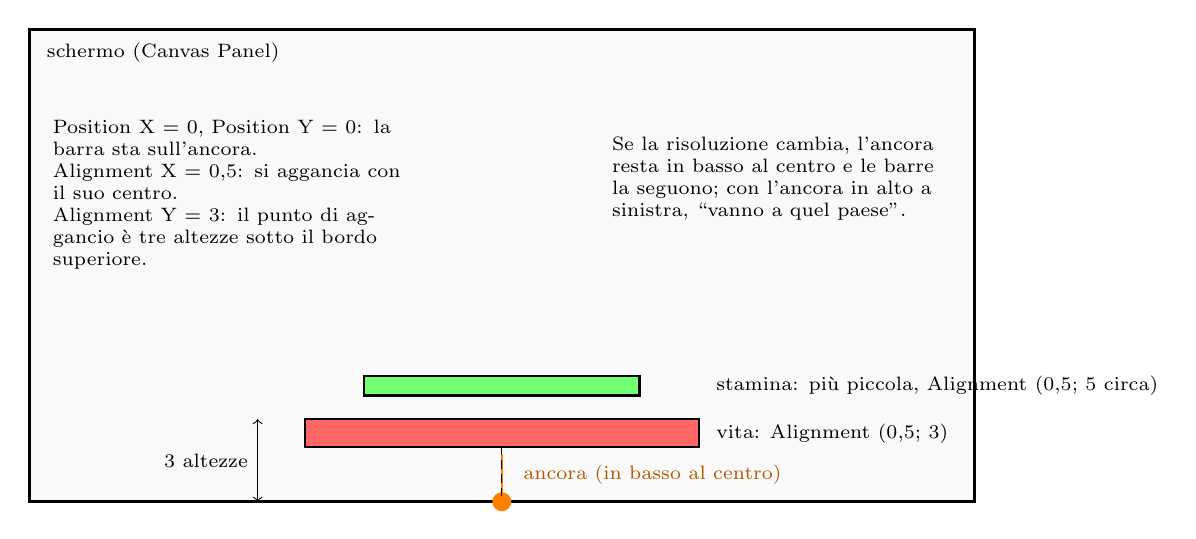
\begin{tikzpicture}[font=\footnotesize, x=1cm, y=1cm]
  % schermo
  \draw[very thick, fill=gray!5] (0,0) rectangle (12,6.0);
  \node[anchor=north west, font=\scriptsize] at (0.1,5.95) {schermo (Canvas Panel)};
  % ancora in basso al centro
  \fill[orange] (6,0) circle (0.12);
  \draw[orange, thick] (6,0) -- (6,0.6);
  \node[orange!70!black, font=\scriptsize, anchor=west] at (6.15,0.35) {ancora (in basso
    al centro)};
  % barra vita: alignment 0.5, 3 -> altezza 0.35 -> bordo superiore a 3*0.35=1.05
  \draw[thick, fill=red!60] (3.5,0.70) rectangle (8.5,1.05);
  \node[font=\scriptsize, anchor=west] at (8.6,0.87) {vita: Alignment (0,5; 3)};
  % barra stamina: posizione indicativa
  \draw[thick, fill=green!55] (4.25,1.35) rectangle (7.75,1.6);
  \node[font=\scriptsize, anchor=west] at (8.6,1.48) {stamina: più piccola, Alignment
    (0,5; 5 circa)};
  % pivot
  \draw[densely dashed] (6,0.70) -- (6,0);
  \draw[<->, thin] (2.9,0) -- node[left, font=\scriptsize]{3 altezze} (2.9,1.05);
  \node[font=\scriptsize, text width=4.6cm, align=left] at (2.6,3.9) {Position X = 0, Position
    Y = 0: la barra sta sull'ancora.\\ Alignment X = 0,5: si aggancia con il suo centro.\\
    Alignment Y = 3: il punto di aggancio è tre altezze sotto il bordo superiore.};
  \node[font=\scriptsize, text width=4.4cm, align=left] at (9.6,4.1) {Se la risoluzione
    cambia, l'ancora resta in basso al centro e le barre la seguono; con l'ancora in alto
    a sinistra, ``vanno a quel paese''.};
\end{tikzpicture}
\caption{Ancore, posizione e allineamento di un widget nel Canvas Panel. La posizione si
misura dall'ancora, l'allineamento sposta il punto dell'elemento che si aggancia
all'ancora, in frazioni della sua dimensione. Schema ricostruito; proporzioni indicative.}
\label{ue11:fig:ancore}
\end{figure}

\paragraph{Approfondimento: ancore e Percent nel libro.} Romero e Sewell (capitolo 7):
``poiché le dimensioni e i rapporti degli schermi possono variare, vogliamo assicurarci
che gli elementi della UI restino nella stessa posizione relativa sullo schermo. Le ancore
servono a definire la posizione desiderata di un widget sul canvas, indipendentemente
dalla dimensione dello schermo.'' Il simbolo a forma di fiore che si vede nel Designer si
chiama \emph{Anchor Medallion}, ``e rappresenta la posizione dell'ancora dell'elemento
selezionato''; la seconda edizione aggiunge che si può anche trascinare direttamente il
fiore nel punto voluto, o espandere \emph{Anchors} per i controlli di precisione. Uno dei
quesiti di fine capitolo chiede se ``i valori X e Y della posizione di un elemento in un
canvas sono sempre relativi all'angolo in alto a sinistra dello schermo'': la risposta è
no, sono relativi all'ancora, che è esattamente ciò che Guido ha scoperto. Sul Percent:
``l'intervallo dei valori va da 0,0 (vuota) a 1,0 (piena)''. Il libro anticipa anche il
motivo per cui serve una divisione: le sue variabili di vita e stamina hanno valore di
default 1,0 proprio perché ``questo valore è usato dai UI meters, che mostrano il grado di
riempimento fra 0,0 e 1,0''. La lezione invece tiene la vita in punti (10) e la stamina in
centesimi (100), e converte al momento di disegnare.

% ---------------------------------------------------------------------
\section{L'HUD sullo schermo: Initialize, Create Widget e Add to Viewport}
\label{ue11:sec:viewport}

\paragraph{L'evento d'inizializzazione.} Nel \textbf{Graph} del widget (``in alto a
destra, Designer e Graph: se clicchi su Graph vai direttamente là''), si tolgono gli eventi
predefiniti e si crea un \textbf{Custom Event}: \textbf{InitializeHealthBar}. Gli serve un
input, ``la referenza stessa al player'': nei Details dell'evento, sotto \emph{Inputs}, il
più, nome \textbf{PlayerRef}, tipo la classe del proprio personaggio (``io ho BP\_Bot2,
ma deve essere il nome del vostro character''), \textbf{Object Reference}: ``quella
azzurra, deve essere azzurra''. A che serve? ``Chiamerà l'Event Dispatcher'': il personaggio
dirà ``ehi, fammi esistere questa UI, mettimela sullo schermo'', e a quel punto bisogna
``bindare l'evento al fatto di inizializzare la barra, quindi dargli subito il valore di
quant'è la vita''. (A chi chiede ``com'è che sotto c'è la freccia bianca?'': è l'evento con
il suo input, che si aggiunge dai Details.)

\paragraph{Il Begin Play del personaggio.} ``Innanzitutto, buona regola, dobbiamo passargli
la PlayerRef.'' In BP\_Bot2, all'\textbf{Event BeginPlay}: ``quando il gioco inizia,
vogliamo che l'HUD, quindi questa schermata, la sua Progress Bar e tutto quanto, vada a
esistere nel mondo, nella nostra viewport''.
\begin{enumerate}
  \item \textbf{Create Widget} (``scusate, non \emph{Add}: è Create Widget''). Il pin
        \textbf{Class} chiede ``la tipologia di asset che andiamo a creare'': WB\_HUD;
  \item il \textbf{Return Value} si promuove a variabile, \textbf{AsHUD}: ``non lo useremo,
        però è una buona cosa sempre fare una referenza, perché magari volete comunicare
        altre volte con il nostro HUD e cambiargli dei valori'';
  \item ``questo lo crea, ma non lo mette nella viewport'': serve \textbf{Add to Viewport},
        con l'HUD come target. In Play, ``ecco a voi che la nostra barra rossa è apparsa
        a schermo'';
  \item infine, dalla variabile AsHUD, la chiamata a \textbf{InitializeHealthBar}, con
        \textbf{PlayerRef} collegato a un \textbf{Get a Reference to Self} (``fate
        \emph{self}, vi appare Get a Reference to Self''). ``Abbiamo detto: ehi, aggiungi
        questo widget alla viewport e inizializza.''
\end{enumerate}
(Durante questa parte il docente ha qualche problema di connessione: ``scusa, ho visto
adesso la chat; sto avendo problemi, devo fare un po' di manutenzione''.)

% ---------------------------------------------------------------------
\section{Il collegamento: Bind Event e Set Percent}
\label{ue11:sec:bind}

\paragraph{Il Bind.} ``Ci manca ovviamente la funzione collegata'': bisogna fare in modo
che l'inizializzazione \emph{agganci} l'aggiornamento della barra all'aggiornamento della
vita. Nel Graph del widget, dopo InitializeHealthBar, dal pin PlayerRef: \textbf{Bind
Event to E\_UpdateHealth} (la trascrizione sente ``bind e update''). Compilando dà errore,
``giustamente'': ``mi serve un evento: che evento devo collegare al fatto che io aggiorno la
mia variabile Health?''. L'evento si crea così: dal pin rosso \textbf{Event} del Bind si
trascina un filo e si sceglie \textbf{Add Custom Event}. ``Mi raccomando: non fate un
Custom Event esterno, tirate fuori proprio da Event e fate Custom Event, perché vi tira
fuori e si porta dietro i due valori che gli abbiamo dato di input, cioè CurrentHealth e
MaxHealth.'' Il nome: \textbf{UpdateHealthBar}.

\paragraph{Che cosa succede.} Una studentessa riassume: ``quindi quando viene
inizializzato, in automatico fa anche Update Health?''. ``Esatto.'' Quando il gioco
inizia, l'HUD ``binda l'evento di aggiornare la barra al nostro Update Health, cioè al
valore numerico che si aggiorna''. ``Creiamo il collegamento'': da quel momento, ``quando si
aggiorna effettivamente il nostro numero, la nostra variabile, allora avviene anche
l'update della barra''.

\paragraph{L'evento senza posti.} ``A me il Bind Event non me l'ha dato'': la studentessa
aveva creato prima, per sbaglio, un Custom Event separato e l'aveva collegato al Bind;
cancellato quello, il Bind risultava ``ancora delegato''. ``Elimina quello che hai
adesso; tira fuori da Event, Custom Event.'' La spiegazione: un Custom Event creato a mano
``non ti dà quei valori di input, CurrentHealth e MaxHealth''; ``questo qua deve essere
creato tramite il collegamento, perché noi gli abbiamo messo degli input''. ``Non deve
essere vuoto: si deve portare dietro i posti per la CurrentHealth e la MaxHealth.
Ricordiamoci il camion.''

\paragraph{Rinominare la barra.} ``Per ordine'': nel Designer, nella \textbf{Hierarchy}
(``ci permette di avere tutte le nostre cosine che abbiamo messo nella UI, tutte belle
elencate''), si seleziona la Progress Bar e con \textbf{F2} la si rinomina
\textbf{ProgressBar\_Health}.

\paragraph{Set Percent.} Nel Graph, la variabile ProgressBar\_Health si trascina
nell'evento UpdateHealthBar e da lei si tira fuori \textbf{Set Percent}. ``In questo caso
però si tratta di una percentuale, quindi è un valore da 0 a 1'': il valore è
\textbf{CurrentHealth diviso MaxHealth}, i due pin dell'evento in un \textbf{Divide}. In
Play, ``la mia barra diminuisce sempre di più, e boom, eccoci qua''
(figure~\ref{ue11:fig:hudgraph} e~\ref{ue11:fig:catena}).

\begin{figure}[htbp]
\centering
\begin{tikzpicture}[font=\scriptsize,
  ue11node/.style={draw, thick, rounded corners=4pt, align=center, fill=gray!8,
                  minimum height=0.9cm, text width=2.0cm},
  ue11ev/.style={ue11node, fill=red!12},
  ue11var/.style={ue11node, fill=blue!10, rounded corners=8pt},
  ue11exec/.style={-{Stealth[length=2.5mm]}, very thick, black!80},
  ue11data/.style={-{Stealth[length=2mm]}, thick, blue!60!black}]
  \node[font=\scriptsize\bfseries, anchor=west] at (-1.0,1.0) {BP\_Bot2, Event Graph};
  \node[ue11ev, text width=1.5cm] (bp) at (0,0) {\textbf{Event BeginPlay}};
  \node[ue11node, text width=1.7cm] (cw) at (2.4,0) {\textbf{Create Widget}\\Class:
    WB\_HUD};
  \node[ue11var, text width=1.4cm] (sh) at (4.7,0) {\textbf{Set}\\AsHUD};
  \node[ue11node, text width=1.6cm] (av) at (6.9,0) {\textbf{Add to Viewport}};
  \node[ue11node, fill=yellow!20, text width=2.5cm] (ih) at (9.7,0)
    {\textbf{Initialize\-Health\-Bar}\\PlayerRef: Self};
  \node[ue11node, fill=yellow!20, text width=2.5cm] (is) at (13.0,0)
    {\textbf{Initialize\-Stamina\-Bar}\\PlayerRef: Self (più tardi)};
  \draw[ue11exec] (bp) -- (cw); \draw[ue11exec] (cw) -- (sh);
  \draw[ue11exec] (sh) -- (av); \draw[ue11exec] (av) -- (ih);
  \draw[ue11exec, dashed] (ih) -- (is);
  \node[font=\scriptsize\bfseries, anchor=west] at (-1.0,-1.6) {WB\_HUD, Graph};
  \node[ue11ev, text width=2.5cm] (ini) at (0.3,-2.7) {\textbf{Initialize\-Health\-Bar}\\
    Custom Event, input PlayerRef};
  \node[ue11node, text width=2.5cm] (bind) at (3.9,-2.7) {\textbf{Bind Event to
    E\_UpdateHealth}\\Target: PlayerRef};
  \node[ue11ev, text width=2.5cm] (upd) at (8.3,-2.7) {\textbf{Update\-Health\-Bar}\\
    CurrentHealth, MaxHealth};
  \node[ue11node, text width=1.6cm] (div) at (10.9,-4.4) {\textbf{Divide}\\Current /
    Max};
  \node[ue11node, text width=2.6cm] (sp) at (12.4,-2.7) {\textbf{Set Percent}\\Target:
    ProgressBar\_Health};
  \draw[ue11exec] (ini) -- (bind);
  \draw[ue11data, red!60!black] (bind) -- node[below]{Event} (upd);
  \draw[ue11exec] (upd) -- (sp);
  \draw[ue11data] (upd.south) |- (div.west);
  \draw[ue11data] (div.north) -- node[right]{In Percent} (sp.south -| div.north);
\end{tikzpicture}
\caption{I due lati dell'HUD. In alto, il personaggio crea il widget, se lo salva, lo
aggiunge alla viewport e gli passa una referenza a se stesso. In basso, il widget usa
quella referenza per legare il proprio evento UpdateHealthBar all'Event Dispatcher del
personaggio: da lì in poi, ogni Call E\_UpdateHealth esegue Set Percent. La chiamata
tratteggiata si aggiunge con la stamina. Schema ricostruito.}
\label{ue11:fig:hudgraph}
\end{figure}

\begin{figure}[htbp]
\centering
\begin{tikzpicture}[font=\footnotesize,
  ue11node/.style={draw, thick, rounded corners=4pt, align=center, fill=gray!8,
                  minimum height=1.0cm, text width=2.5cm},
  ue11exec/.style={-{Stealth[length=2.5mm]}, very thick, black!80}]
  \node[ue11node, fill=orange!15] (pr) at (0,0) {\textbf{BP\_Projectile}\\{\scriptsize
    Sphere Trace, Break Hit Result}};
  \node[ue11node, fill=orange!15] (ad) at (3.4,0) {\textbf{Apply Damage}\\{\scriptsize
    Hit Actor, Base Damage 1}};
  \node[ue11node, fill=red!12] (any) at (6.8,0) {\textbf{Event Any\-Damage}\\{\scriptsize
    in BP\_Bot2}};
  \node[ue11node, fill=blue!10] (hp) at (10.2,0) {\textbf{CurrentHealth}\\{\scriptsize
    Subtract, Clamp, Set}};
  \node[ue11node, fill=yellow!20] (call) at (10.2,-2.2) {\textbf{Call
    E\_UpdateHealth}};
  \node[ue11node, fill=green!10] (ev) at (6.8,-2.2) {\textbf{Update\-Health\-Bar}\\
    {\scriptsize in WB\_HUD (legato)}};
  \node[ue11node, fill=green!10] (pb) at (3.4,-2.2) {\textbf{Set Percent}\\{\scriptsize
    Current / Max}};
  \node[ue11node, fill=green!20] (bar) at (0,-2.2) {\textbf{barra rossa}\\{\scriptsize
    sullo schermo}};
  \draw[ue11exec] (pr) -- (ad); \draw[ue11exec] (ad) -- (any);
  \draw[ue11exec] (any) -- (hp); \draw[ue11exec] (hp) -- (call);
  \draw[ue11exec] (call) -- (ev); \draw[ue11exec] (ev) -- (pb);
  \draw[ue11exec] (pb) -- (bar);
  \node[font=\scriptsize, text width=13cm, align=center] at (5.1,-3.6) {Il proiettile non
    sa nulla della UI, e la UI non sa nulla del proiettile: ognuno parla solo con il
    personaggio.};
\end{tikzpicture}
\caption{Il percorso completo di un colpo, dal proiettile alla barra. Il sistema di danno
di Unreal collega il proiettile al personaggio; l'Event Dispatcher collega il personaggio
all'HUD. Schema riassuntivo.}
\label{ue11:fig:catena}
\end{figure}

\paragraph{I problemi dei presenti.} ``Ci siete, ragazzi?'' Tre casi.
\begin{itemize}
  \item \textbf{Set Percent introvabile.} ``Non mi dà il Set Percent'', e nemmeno i
        Details per cercarlo. Primo controllo: nel Designer, la Progress Bar deve avere la
        spunta \textbf{Is Variable}, altrimenti nel Graph non esiste come variabile. I
        Details mancanti si riaprono da \textbf{Window}, \textbf{Details}. La spunta c'era;
        il vero errore è un altro: lo studente cercava Set Percent trascinando da un altro
        nodo. ``Ah, ok, lo facevo da qua'': Set Percent si trova solo \emph{tirando fuori
        dalla variabile} ProgressBar\_Health, che va presa dalla sezione \emph{Variables}
        (``se non ce l'hai, c'è la tendina'') e trascinata nel grafo. Per la divisione:
        ``tiri fuori dalla CurrentHealth e fai lo slash'', oppure si scrive
        \emph{divide}; poi ``questo diviso per quell'altro''.
  \item \textbf{La torretta che non spara}, a un'altra studentessa: rimandata alla pausa.
  \item \textbf{La barra che non scende.} ``La vita la perdo, perché poi respawno; tuttavia
        graficamente non scende la barra.'' Il Bind c'è, il danno è 1 (``l'ho messo come
        variabile''), la vita è 10. Un Print String dopo il Set Percent, ``attaccalo a In
        String'' (``collega quello verde a quello rosa''), non stampa niente. Allora
        \textbf{F9} sull'evento UpdateHealthBar: ``dice: sta facendo questo evento?''. Il
        breakpoint non scatta. In BP\_Bot2 si scopre perché: nel Begin Play mancava la
        chiamata a \textbf{InitializeHealthBar} dopo Add to Viewport. ``Non stai dicendo al
        gioco che, quando inizia, se io ho dato la vita, mi aggiorni pure la barra.'' Si
        aggiunge da AsHUD, con Self nel PlayerRef; si toglie il breakpoint (``se no te lo
        farà ogni volta''). ``Perfetto, grazie.''
\end{itemize}

\paragraph{Il portatile surriscaldato.} Un altro studente non riesce a seguire: ``sta
andando a scatti'', ``è troppo surriscaldato il computer''. Il consiglio, per tutti: ``per
chi ha un portatile, prendetevi quelle basette con le ventole'': ``col portatile quello
diventa un vulcano a un certo punto''. Lo studente ce l'ha già: ``ah, ok. Quindi sta proprio
andando pesantissimo''. ``Lascialo riposare il nostro soldato, tranquillo: tanto poi c'è la
registrazione.''

\paragraph{Approfondimento: Bind Event contro i Binding del libro.} Qui la lezione e il
libro scelgono due strade diverse, e vale la pena capire perché. Romero e Sewell
(capitolo 7) usano i \textbf{Binding} delle proprietà: accanto al campo \emph{Percent}
della Progress Bar c'è un pulsante \emph{Bind}; scegliendo \emph{Create Binding}, l'editor
crea una funzione che restituisce il valore, in cui gli autori mettono \emph{Get Player
Character}, \emph{Cast To FirstPersonCharacter} e il Get della vita. ``I Binding ci danno
la possibilità di legare variabili o funzioni di un Blueprint a un Widget. Ogni volta che
la variabile o la funzione è aggiornata, il cambiamento si riflette automaticamente nel
Widget.'' Il prezzo, per il funzionamento generale di UMG, è che una funzione di Binding
viene valutata \emph{a ogni frame}, che il valore sia cambiato o no (e, nell'esempio del
libro, con un cast a ogni valutazione). Lo schema della lezione è \emph{a eventi}: la barra
si aggiorna solo quando il personaggio chiama E\_UpdateHealth, cioè quando la vita cambia
davvero. Per due barre la differenza di prestazioni è trascurabile; diventa importante
negli HUD con molti elementi, e soprattutto rende esplicito \emph{chi} aggiorna \emph{che
cosa}. Sul Bind Event, invece, il libro (capitolo 4) dice la stessa cosa del docente:
``c'è un nodo Bind Event che lega un evento a un altro evento o a un Event Dispatcher, che
può stare in un altro Blueprint. Quando un evento è chiamato, tutti gli altri eventi legati
a lui sono chiamati'', e il Custom Event si crea trascinando ``dal pin rosso del nodo Bind
Event'' e scegliendo \emph{Add Custom Event}. Un dettaglio generale: un Custom Event creato
dal pin riceve automaticamente la \emph{firma} del dispatcher (i suoi input); se in seguito
si aggiungono input al dispatcher, gli eventi legati vanno aggiornati, e l'editor lo segnala
con un errore di firma alla compilazione.

% ---------------------------------------------------------------------
\section{La seconda barra e la corsa}
\label{ue11:sec:corsa}

``Abbiamo un quarto d'oretta. Sai che facciamo? Andiamo a creare la nostra barra della
stamina e facciamo insieme la stamina, così dopo magari facciamo qualcos'altro, che è il
menu in questo caso.''

\paragraph{La barra copiata.} ``Più che metterne una nuova'', nel Designer di WB\_HUD si
copia la barra della vita con \textbf{Ctrl+C} e \textbf{Ctrl+V}. La copia ha ancora
l'ancora in basso al centro; si azzerano le posizioni, \textbf{Alignment} X a \textbf{0,5}
e Y più alto, perché stia sopra la barra rossa (il docente dice ``non 3, ma la mettiamo
tipo a 2, e facciamo 5'', poi ``facciamo 5''), la si fa ``un pochino più piccola'' (con i
campi della dimensione, ``1,8, ma sì, 2'': ``questi rettangolini servono per essere un po'
più precisi''), e verde. ``Se volete, ragazzi, sbizzarritevi: i colori, proprio pastelli in
mano, fate come volete.''

\paragraph{InitializeStaminaBar.} ``Facciamo la stessa identica cosa per l'inizializzazione
della barra'': nel Graph, un altro Custom Event, \textbf{InitializeStaminaBar}, con lo
stesso input \textbf{PlayerRef} (``fortunatamente, se avete già fatto l'input, vi dice già:
ce l'ho, PlayerRef''). ``Per adesso lo lasciamo così, perché dobbiamo creare un altro
Event Dispatcher, che sarà invece l'update della stamina.''

\paragraph{IA\_Run.} Torniamo nel bot: ``dobbiamo far correre il nostro player''. Serve
un'\textbf{Input Action} nuova, \textbf{IA\_Run}, accanto a IA\_Look, IA\_Move e IA\_Jump;
la si era fatta la volta scorsa per il cavaliere, e ``fortunatamente'' basta una volta:
``questa è la bellezza del context: la mappatura degli input è separata dal player'', e
``la posso passare da player a player''. Per chi non ce l'ha:
\begin{enumerate}
  \item da un'azione qualsiasi, tasto destro, \textbf{Show in Folder View}; si
        \textbf{duplica} IA\_Jump e la si chiama IA\_Run. ``Se non sbaglio, Jump e Run
        sono uguali'': entrambe hanno un valore booleano (\emph{Digital});
  \item nell'\textbf{IMC} (\emph{Input Mapping Context}), il più, IA\_Run, e nella
        tendina la \textbf{tastiera}: ``cliccate sulla tastiera, premete Shift'', ``in modo
        da dire: guarda che questo è l'input collegato alla corsa''.
\end{enumerate}
``Io l'ho spiegato molto velocemente, perché so che, se qualcuno nel caso non avesse
visto, poi mi dica.''

\paragraph{Gli stati dell'evento.} Nel bot, l'evento \textbf{IA\_Run} mostra le sue uscite
(\emph{Triggered}, \emph{Started}, \emph{Ongoing}, \emph{Canceled}, \emph{Completed});
``in questo caso ci interesseranno solamente lo \textbf{Started} e il
\textbf{Completed}'': l'inizio e la fine della pressione.

\paragraph{Camminare di default.} ``Per dire già che il player deve camminare di default'',
si guarda il Blend Space del bot: la camminata è a 250, ``facciamo 300, un po' più alto''.
Nel \textbf{Character Movement}, categoria \emph{Character Movement: Walking},
\textbf{Max Walk Speed} a \textbf{300}: ``da adesso in poi il nostro character camminerà''.
(Se i passi non suonano, ``lo fixiamo poi'': il docente aveva aggiunto i suoni dei passi
anche all'animazione di camminata prima della lezione, ``perché prima solamente
correvamo''.)

\paragraph{Correre.} Due \textbf{Set Max Walk Speed}, entrambi con il Character Movement
come target (``ricordatevi di tutti e due di collegarli''): uno allo \textbf{Started}, a
\textbf{500}, uno al \textbf{Completed}, a \textbf{300}. (Il docente dice prima 600, poi
``500 era? Facciamo 500, va bene'', il valore massimo del Blend Space.) In Play: ``cammino;
Shift, corro; Shift, lascio''. ``Sicuramente possiamo mettere un po' di smooth
all'animazione'', con un \emph{blend in} e un \emph{blend out}: ``questo è un fix che
possiamo fare dopo, tranquillamente''.

\paragraph{La stamina di Dark Souls.} ``Qualcuno di voi ha in mente Dark Souls? La stamina
di Dark Souls, o in generale, molto spesso la stamina funziona in questo modo'': ``viene
persa durante un quantitativo di tempo, se si fa una certa azione, in questo caso correre:
viene levata gradualmente'', e quando l'azione smette ritorna su piano piano. ``Visto che
parliamo di tempo, useremo due \textbf{timer}'', come per la torretta, ``per far sì che
queste due cose vadano a scalare nel tempo''. Mancano cinque minuti alla pausa: ``facciamo
adesso un piccolo timer, oppure vogliamo andare già in pausa?''. Si va in pausa: ``la
prova è 25'', ``facciamo 17 e 55 e ci rivediamo''.

\paragraph{Approfondimento: lo sprint nel libro.} Romero e Sewell costruiscono lo sprint nel
capitolo 6 con il sistema di input precedente (l'\emph{Action Mapping} ``Sprint'' sul
tasto Shift sinistro, gli eventi \emph{Pressed} e \emph{Released}) e due \emph{Set Max
Walk Speed}, esattamente come la lezione con l'Enhanced Input (Started e Completed). Nel
capitolo 8 fanno un'osservazione di design che spiega perché la stamina serve: senza un
vincolo, ``non ci sarebbe niente a scoraggiare il giocatore dal tenere sempre premuto
Shift mentre si muove''; ``se un'opzione è così attraente che il giocatore si sente
costretto a usarla sempre, allora non aumenta il numero di scelte interessanti''. ``Dal
punto di vista del giocatore, il risultato sarebbe lo stesso se aumentassimo semplicemente
la velocità di base fino a quella dello sprint.'' La stamina trasforma lo sprint in una
\emph{risorsa}: correre ora significa non poter correre fra poco. È la stessa logica della
stamina di Dark Souls, dove la stessa barra è condivisa da corsa, schivata, parata e
attacco, e ogni scelta ha un costo.

% ---------------------------------------------------------------------
\section{La pausa: le torrette e i bot degli studenti}
\label{ue11:sec:pausa}

La pausa, come spesso in questo corso, diventa uno sportello di correzioni. Il docente
resta collegato e guarda i progetti uno alla volta, in condivisione di schermo
(``quando condividi, fai \emph{condividi schermo}, non condividere Unreal, perché è più
facile: stiamo schermando più grande'').

\paragraph{Lo Shift che non corre.} Il primo studente: ``se mi muovo normalmente cammina,
se premo Shift non corre''. ``Allora c'hai qualche cosa che non va nell'IA\_Run.'' La cosa
resta in sospeso: il problema dello stesso tipo tornerà, più grave, alla fine della lezione
(sezione~\ref{ue11:sec:barrastamina}).

\subsection{La torretta di Tommaso}

``Io entro, mi vede, ma non spara.'' Il tag Player c'è.
\begin{enumerate}
  \item \textbf{La collisione della mesh del bot}: ``non l'avevo messa''. Mesh, Collision,
        Custom, Detection Turret in Block (e Projectile Trace: ``va benissimo''). Ora la
        torretta lo segue, ma non spara.
  \item \textbf{Il Trace Channel}: nella torretta, il trace di rilevamento usava il canale
        sbagliato. ``Cambia Trace Channel'' a \textbf{Detection Turret} (``no, no, torna
        indietro; Ctrl+Z''). ``Ok, benissimo.''
  \item \textbf{La funzione dello spawn}: alla torretta di Tommaso manca proprio la
        funzione che fa nascere il proiettile. Il docente gliela passa con ``un
        trucchettino'': ``la cosa bella dei Blueprint è che puoi incollarli in un file di
        testo, copiarli tutti quanti''. Seleziona i nodi della sua funzione, Ctrl+C, li
        incolla in un file \emph{.txt} (``Fix, funzione Spawn'') e glielo manda su
        Discord, in privato. Tommaso scarica il file, ne copia tutto il testo e lo incolla
        con Ctrl+V nel grafo di Unreal: i nodi ricompaiono.
  \item \textbf{Sistemare l'incollato}: ``adesso c'hai degli errori, eh? Perché devi
        sistemarlo''; ``prima fix, poi ordina''. La funzione si rinomina con F2
        \textbf{Spawn Projectile}. Servono i due punti di uscita: nei Components, Add,
        due \textbf{Scene Component}, \textbf{ProjectileSpawn1} e \textbf{ProjectileSpawn2}
        (copiati con Ctrl+C e Ctrl+V), agganciati al \textbf{cannone} della torretta e
        spostati ``ai bocchettoni della mesh'', ``poco fuori la canna''.
  \item \textbf{Lo Spawn Actor rifatto}: il nodo incollato dà un errore sull'\emph{Spawn
        Actor} (``non ti spawno nessun actor''); l'errore sull'\emph{Instigator} invece
        ``va bene, non ci interessa''. ``Facciamo prima'': si cancella e si rifà
        \textbf{Spawn Actor from Class}; tasto destro sullo \emph{Spawn Transform},
        \textbf{Split Struct Pin}; si collegano Location e Rotation dei due Scene; la
        \textbf{Class} è il proiettile, BP\_Projectile.
  \item Una curiosità di Tommaso, nel frattempo: ``pure la barra della stamina, io gli ho
        dato un colore, ma me la dà grigia''. ``Forse è vuota'': il \emph{Percent} è a 0,
        e una Progress Bar vuota mostra solo lo sfondo. ``Faccio 1.''
  \item \textbf{Chiamare la funzione}: la torretta ancora non spara, ``perché non
        spawni'': nello \emph{Shoot}, al posto delle due vecchie chiamate, va chiamata la
        nuova \textbf{Spawn Projectile}.
  \item \textbf{Le collisioni della torretta}: il proiettile non deve fermarsi sulla
        torretta stessa. Sul cannone, sulla sfera di rilevamento e sul pivot, il canale
        Projectile Trace va su \textbf{Ignore} (``devi ignorare tutto, anche il pivot'').
\end{enumerate}
La torretta di Tommaso ancora non spara; ``aspetta, adesso facciamo fare Lucrezia, che è
un po' che aspetta''. Si riprenderà dopo la pausa.

\subsection{Il bot di Lucrezia, risolto}

\paragraph{Il Validated Get sulla variabile sbagliata.} Con Shift il bot di Lucrezia ora
``va più veloce'': ``quello almeno va benissimo''; quindi il personaggio si muove, ``è un
problema di animazioni''. Il docente esclude un doppio scheletro (``non vorrei che avessi
un doppio scheletro e te l'avessi fatto su un altro'': ne ha uno solo), poi mette un
Print String sull'uscita \textbf{Is Not Valid} del Validated Get, all'inizio dell'Update.
Stampa: ``ecco il nostro problema: la referenza a questo actor non è valida''. Il motivo:
``hai messo nel Validated Get la variabile del PB\_Bot, non del BP\_Bot, che sono due
diverse'': nell'Animation Blueprint c'erano due variabili quasi omonime, e il Validated
Get controllava quella che l'Initialize non riempiva mai. Si cancella, si prende la
variabile giusta (\textbf{AsBP\_Bot}), tasto destro, \textbf{Convert to Validated Get}, si
ricollega. ``Dovremmo aver scoperto l'arcano.'' ``Era lui.''

\paragraph{La regola di ritorno all'Idle.} Ora il bot anima, ma ``continua a camminare sul
posto'' quando si ferma. Nella State Machine, la regola Walk $\rightarrow$ Idle era
\emph{GroundSpeed $<$ 0}: ``attenzione, non è minore, è \textbf{minore o uguale}'',
perché una velocità negativa non esiste (la lunghezza di un vettore è sempre $\ge 0$), e con
il minore stretto la regola non è mai vera (``solo se sarà meno uno la velocità'').

\paragraph{Il Lean, di nuovo.} Correndo e girando, il bot ``non si inclina tantissimo'':
la stessa correzione fatta a inizio lezione (``come abbiamo fatto anche con Tommaso'': la
trascrizione attribuisce qui a Tommaso il Lean corretto all'inizio). Nel Blend Space i
campioni da $\pm 10$ a $\pm 1$, poi l'asse, nelle \emph{Axis Settings} dei Details, da $-1$
a 1. ``Ecco che si piega leggermente.''

\paragraph{La torretta di Lucrezia.} Poi la torretta, aperta con \emph{Edit BP\_Turret} dal
livello (``lo fai diretto''). ``Questo è un po' incasinato, eh? Vabbè, tranquillo.'' In
ordine:
\begin{itemize}
  \item \textbf{Begin Overlap}: il fix di inizio lezione, Get Player Pawn al posto
        dell'Other Actor nel Set di PlayerTarget;
  \item \textbf{Move Turret} (la rotazione verso il bersaglio): il nodo di rotazione
        usato era un altro, e si sostituisce con \textbf{Find Relative Look at
        Rotation}, che vuole uno \emph{Start Transform} (``non ti serve il Get Actor
        Rotation, ma devi invocare il \textbf{Get Actor Transform}'', ``pinnetto
        arancione per pinnetto arancione'') e una \emph{Target Location}, il \textbf{Get
        Actor Location} del PlayerTarget. Del risultato, con \emph{Split Struct Pin}, si
        usa la \textbf{Z} (lo Yaw) come \emph{Target} dell'interpolazione; un vecchio
        ``meno'' non serve più; nel \emph{Delta Time} va \textbf{Get World Delta Seconds}.
        La trascrizione, qui, è troppo frammentaria per ricostruire il grafo nodo per nodo;
        il senso è quello della rotazione della torretta costruita nelle lezioni
        precedenti;
  \item \textbf{Shoot}: Branch, Sequence, i due \emph{Do Once} con lo Spawn Projectile e il
        Delay, il \emph{Fire Rate}: ``va benissimo'';
  \item un secondo \emph{On Component Begin Overlap} rimasto da una prova (``probabilmente
        una cosa che avevo cancellato'', ``l'avevo spostata''): si elimina; l'\emph{End
        Overlap} e il Tick si tengono;
  \item \textbf{il tag}: la torretta ancora non la segue. Il tag Player era stato messo nei
        \emph{Component Tags} della mesh: ``attenzione, non della mesh, ma quello sotto'':
        i \textbf{Tags} dell'\emph{actor}, e con la stessa maiuscola.
\end{itemize}

\paragraph{Il proiettile assassino.} Ora la torretta spara (``sei un po' alta''), ma
emergono tre problemi del proiettile, uno dopo l'altro.
\begin{enumerate}
  \item I proiettili urtano la camera del personaggio: sulla \emph{Sphere} del proiettile,
        Collision, \textbf{Camera} su \textbf{Ignore}.
  \item I proiettili ``non si distruggono se il character gli va addosso'': la Sphere
        Trace aveva \textbf{Radius 0}, ``quindi è grande niente''. A \textbf{20}.
  \item Ora un colpo e il bot ``si blocca proprio tutto'', anche se la vita non è finita.
        Nel proiettile, dopo il colpo, c'era un \textbf{Destroy Actor} con l'\emph{Hit
        Actor} come target (un ramo chiamato \emph{Kill Target}): ``se colpisco qualcosa,
        distruggimi quello che ho colpito''. Il proiettile cancellava il personaggio dal
        mondo. Al suo posto: \textbf{Apply Damage} (Hit Actor nel Damaged Actor, Base
        Damage 1), e poi \textbf{Destroy Actor} senza target, cioè \emph{self}: ``quando
        collide con qualcosa, distruggi il proiettile: si autodistrugge''.
\end{enumerate}

\paragraph{La vita a zero e la NewVar.} Ora il bot ``muore praticamente subito'': la
\textbf{MaxHealth} aveva default 0, e il Clamp riduceva a zero qualunque vita. MaxHealth a
10. Poi il contrario: il primo colpo toglie vita, ``poi adesso è immortale''. Nell'Event
AnyDamage c'era un Set su una variabile \textbf{NewVar}, creata per sbaglio, invece che
sulla CurrentHealth: ``stai praticamente mettendo una variabile nuova come vita''. Si
sostituisce con \emph{Set CurrentHealth}, ricollegando il Return Value del Clamp e il
valore al Branch del minore o uguale. ``Perfetto. Grazie mille.''

\paragraph{Approfondimento: i Blueprint come testo.} Il ``trucchettino'' del file di testo
funziona perché Unreal copia i nodi negli appunti in un formato testuale (lo stesso
formato \emph{T3D} usato per copiare gli actor fra livelli): ogni nodo diventa un blocco
\texttt{Begin Object} \dots\ \texttt{End Object} con la sua classe, la posizione nel grafo,
i valori dei pin e i collegamenti. Incollando quel testo in un altro grafo, anche di un
altro progetto, l'editor ricrea i nodi. È il modo più rapido per condividere un pezzo di
logica in chat o su un forum, ed esistono siti che lo visualizzano come immagine. Il
limite è quello visto a lezione: i riferimenti a variabili, componenti e funzioni del
Blueprint d'origine non esistono nel Blueprint di destinazione, e i nodi che li usano
arrivano ``rotti'' e vanno ricollegati o ricreati (come gli Scene Component e lo Spawn
Actor di Tommaso). Questa è una nozione generale dell'editor, non trattata nei due libri.

% ---------------------------------------------------------------------
\section{Dopo la pausa: ancora la torretta, e gli annunci}
\label{ue11:sec:annunci}

``Eccoci qua, ragazzi, siamo ritornati.'' Tommaso ha provato a togliere e rimettere la
torretta: niente.

\paragraph{L'Event Tick che manca.} ``Io credo che sia \emph{not valid} il PlayerTarget,
probabilmente.'' Il Begin Overlap e il timer sono giusti; ``ah, ti manca il Tick''.
Nell'Event Graph della torretta non c'è l'\textbf{Event Tick} che, a ogni frame, controlla
il bersaglio e spara. Si ricrea: Event Tick, \textbf{Is Valid} (``punto interrogativo,
quello sotto'') con il PlayerTarget come oggetto, e sull'uscita \emph{Is Valid} la
funzione \textbf{Shoot}. La torretta spara.

\paragraph{Fire Rate e velocità.} ``È un po' lento a sparare'': il \textbf{Fire Rate}, fra
le variabili della torretta, è a 0,2 (la trascrizione dice ``02''); il docente suggerisce
un altro valore (``facciamolo 0,7''; il suo è 0,5): dalla trascrizione non si capisce se
il valore sia un intervallo fra i colpi o un'altra cosa nel grafo di Tommaso, e il capitolo
non lo ricostruisce. ``Il proiettile è molto lento'': nel proiettile, il componente
\textbf{Projectile Movement}, \textbf{Initial Speed} e \textbf{Max Speed} a \textbf{1000}.

\paragraph{Il danno che non arriva alla barra.} ``Però non prendo danno.'' Il proiettile ha
l'Apply Damage, ``va bene così''; nel BP\_Bot, però, l'\textbf{Add to Viewport} non era
collegato con il pin di esecuzione all'InitializeHealthBar (``vedi che non è stato
attaccato''). E non basta: nell'Event AnyDamage il Set era su \textbf{MaxHealth} invece che
su CurrentHealth (``ha impostato MaxHealth, non CurrentHealth''). Corretti entrambi:
``vediamo se muoio''. ``Ottimo, perfetto: di solito tutto il casino.''

\paragraph{Il calendario.} Prima di riprendere, gli annunci.
\begin{itemize}
  \item Il \textbf{menu}: ``se non ce la facciamo a fare il menu oggi, lo facciamo la
        prossima volta, e tanto la prossima volta sarà l'ultima lezione che avremo''.
  \item Dopo: ``poi avrete Davide, quindi avrete martedì con me e Davide''; ``poi
        inizierete a fare roba di \textbf{level design}''.
  \item Manca ``un piccolo asset da fare'', le \textbf{porte}: ``possiamo farlo
        tranquillamente la prossima volta, o ve lo lascio come compito, perché sono sicuro
        che lo sapete fare''. ``La timeline l'abbiamo già affrontata'' (il compito è
        descritto nella sezione~\ref{ue11:sec:chiusura}).
\end{itemize}
(``Non stai condividendo?'' ``Ah, ok. Grazie mille, Lucrezia.'')

% ---------------------------------------------------------------------
\section{I due timer della stamina}
\label{ue11:sec:timer}

``E adesso incominciamo a fare questo bellissimo scattino.'' Si torna al bot del docente
(``il proiettile non ci serve più; ci serve botolino''). Il movimento c'è già (500 e 300
sull'IA\_Run); ``abbiamo detto che dobbiamo fare due timer ben distinti: uno che la consuma
e uno che la riporta al suo massimo, piano piano nel tempo''.

\subsection{Il timer che consuma}

\paragraph{Set Timer by Event.} Dopo il Set Max Walk Speed a 500 (lo Started), un
\textbf{Set Timer by Event}.
\begin{itemize}
  \item il pin \textbf{Time} si promuove a variabile, \textbf{TimeStamina}, ``in modo tale
        da avere questa variabile molto più controllabile''; default \textbf{0,05}
        (impostato poco dopo: ``piccola cosa, semplicemente non l'abbiamo impostato''):
        ``questo è il tempo in cui verrà eseguito il timer, ogni 0,05 secondi'';
  \item \textbf{Looping} attivo; \textbf{Max Once Per Frame} attivo;
  \item ``il timer, come abbiamo visto le scorse volte, è un evento collegato'': dal pin
        rosso \textbf{Event} si crea un Custom Event, \textbf{StaminaDeduction}.
\end{itemize}

\paragraph{Le variabili.} ``Lo stesso discorso vale come per la Health'': due Float,
\textbf{CurrentStamina} e \textbf{MaxStamina}, entrambe a \textbf{100}.

\paragraph{StaminaDeduction.} Il corpo è quasi identico a quello della vita:
\begin{enumerate}
  \item CurrentStamina \textbf{Subtract} \textbf{1} (``verrà sottratto di 1 ogni 0,05
        secondi'');
  \item \textbf{Clamp (float)}, fra 0 e MaxStamina (``il nostro valore oscillerà fra un
        minimo di 0 e un massimo di MaxStamina, che è 100'');
  \item \textbf{Set CurrentStamina}: ``farà 99, 98, 97\dots''.
\end{enumerate}
``Questo è lo stesso discorso che vale per la Health, è quasi praticamente medesimo.''

\paragraph{Quando fermarsi: OR con Is Falling.} Poi un \textbf{Branch} (``tenete proprio
B'' e cliccate: la scorciatoia del Branch): se la CurrentStamina è \textbf{minore o uguale
a zero}, si fermerà la corsa (``ancora non abbiamo la funzione, ma la lasciamo così''). E
una piccola accortezza nata ``durante il testing'': ``ci sono dei problemi anche nel caso
noi stiamo cadendo''. ``Io tengo premuto il tasto mentre sto cadendo: non voglio che la
stamina venga consumata, perché non stiamo correndo effettivamente.'' Dal Character
Movement, \textbf{Is Falling} (``ce ne sono due: prendete quello \emph{Nav Movement}'',
quello con l'ingresso blu e l'uscita rossa), e i due booleani in un \textbf{OR Boolean}:
``OR è l'operatore che ci permette di dire \emph{o}: ti fermi se sei minore di zero
\emph{o} se stai cadendo'' (figura~\ref{ue11:fig:deduction}).

\paragraph{Il timer che non si ferma.} Con un Print String della CurrentStamina: ``io
cammino, cammino, comincio a sprintare: i valori scendono. Ma se anche smetto di correre,
i valori continuano a scendere, perché non stoppiamo mai il nostro timer.'' La soluzione è
tenere un \emph{riferimento} al timer: il \textbf{Return Value} di Set Timer by Event (un
\emph{Timer Handle}) si promuove a variabile, \textbf{TimerDeductionStamina}, ``in modo tale
che sia più comodo controllarlo da varie parti''. Al \textbf{Completed} dell'IA\_Run, dopo
il Set Max Walk Speed a 300: un Get di TimerDeductionStamina e \textbf{Clear and Invalidate
Timer by Handle}, ``andiamo a invalidare e fermare il nostro timer''. In Play: ``corro,
smetto di correre: si è fermato a 75''.

\subsection{Il timer che ricarica}

\paragraph{Il secondo timer.} ``Altro problema: se io ricomincio a correre, ripartirà da 75,
non torna piano piano verso 100.'' Quando si smette di correre bisogna ``fare l'opposto'':
subito dopo il Clear, un altro \textbf{Set Timer by Event}, ``sempre in Looping, sempre in
Max Once Per Frame''. Per il tempo il docente usa la stessa TimeStamina, ``ma volendo si può
fare a un valore che volete voi: volete che uno si recuperi più veloce oppure più lento,
sta a voi''. Il suo evento è un Custom Event, \textbf{RegainStamina}: ``non c'è neanche
tanto da sbizzarrirci: è letteralmente la copia di questo''. Si copiano i nodi della
deduzione fino al Set e ``l'unica cosa che andiamo a cambiare è che invece di sottrarre
uno, andiamo ad aggiungere uno'': \textbf{Add} 1, Clamp, Set CurrentStamina.

\paragraph{Fermare anche lui.} Stesso schema al contrario: il Return Value si promuove a
\textbf{TimerRegainStamina}, e allo \textbf{Started} (``quando noi ricominciamo a
correre'') un \textbf{Clear and Invalidate Timer by Handle} su di lui. In Play: ``comincio a
correre, i valori cominciano a scendere; lascio, i valori piano piano risalgono fino a
100''.

\paragraph{Fermarsi a 100.} Ma arrivato a 100, il timer della ricarica continua a girare,
inutilmente. In RegainStamina, dopo il Set, un \textbf{Branch}: se la CurrentStamina è
\textbf{maggiore o uguale} alla MaxStamina, un Clear and Invalidate Timer by Handle su
TimerRegainStamina, ``cioè lo stesso timer che stiamo avendo'': ``se arrivi a 100,
smettila''. ``Non stampo più, si è fermato.''

\subsection{L'evento StopRunning}

\paragraph{La corsa che non finisce.} ``C'è una particolarità'': correndo fino a zero, ``il
nostro character non si ferma, e neanche il timer si ferma'', e il personaggio continua a
correre con la stamina vuota. Serve la funzione di \emph{smettere di correre} anche
\emph{dentro} StaminaDeduction, non solo al rilascio del tasto. ``Per comodità, invece di
fare una funzione a parte'': si stacca il \textbf{Completed} dalla sua catena (Set Max Walk
Speed 300, Clear del timer di deduzione, Set Timer della ricarica), e all'inizio della
catena si mette un nuovo Custom Event, \textbf{StopRunning}. Poi:
\begin{itemize}
  \item il \textbf{Completed} chiama StopRunning;
  \item il ramo \textbf{True} del Branch di StaminaDeduction (stamina $\le$ 0 OR Is
        Falling) chiama StopRunning.
\end{itemize}
``Questa cosa ci serve semplicemente per trasportarci il fatto di \emph{fermati}: vai a
300 di velocità e smettila di sottrarmi la stamina, da questo evento che possiamo
trasportare un po' dappertutto.'' In Play: ``corro, corro, corro, arrivo fino a zero, mi
fermo in automatico'', la stamina risale; ``e poi devo semplicemente ripremere per poter
scattare'' (lo \emph{Started} scatta solo alla pressione). ``Abbiamo fatto il nostro
sistema di stamina'' (figura~\ref{ue11:fig:timer}).

\paragraph{Ricapitolare per chi si è perso.} Una studentessa ha perso il pezzo di
RegainStamina; il docente lo ripete: copiare la catena della deduzione, sostituire il meno
con un più, il Branch con il \emph{maggiore o uguale} (``non mi trova il maggiore'': ``io
ho la tastiera più piccola, non ci ho alcuni segni''; ``allora scrivi \emph{greater
equal}''), MaxStamina e CurrentStamina nei due ingressi, sul True il Clear and Invalidate
Timer by Handle con TimerRegainStamina. Poi StopRunning: ``stacchi da qui il Completed, ci
metti un Custom Event al suo posto, e StopRunning ce lo metti anche al Completed''; la
chiamata, ``di colore azzurro'', ``tiri fuori e fai StopRunning'', anche dopo il Branch.
``Ho recuperato tutto.''

\begin{figure}[htbp]
\centering
\begin{tikzpicture}[font=\footnotesize,
  ue11node/.style={draw, thick, rounded corners=4pt, align=center, fill=gray!8,
                  minimum height=0.9cm, text width=2.1cm},
  ue11ev/.style={ue11node, fill=red!12},
  ue11var/.style={ue11node, fill=blue!10, rounded corners=8pt},
  ue11exec/.style={-{Stealth[length=2.5mm]}, very thick, black!80},
  ue11data/.style={-{Stealth[length=2mm]}, thick, blue!60!black}]
  \node[ue11ev, text width=2.3cm] (ev) at (0,0) {\textbf{Stamina\-Deduction}\\{\scriptsize
    ogni 0,05 s}};
  \node[ue11node, text width=1.9cm] (sub) at (2.6,-2.0) {\textbf{Subtract}\\{\scriptsize
    CurrentStamina $-$ 1}};
  \node[ue11node] (cl) at (5.3,-2.0) {\textbf{Clamp (float)}\\{\scriptsize 0 --
    MaxStamina}};
  \node[ue11var] (set) at (3.1,0) {\textbf{Set}\\{\scriptsize CurrentStamina}};
  \node[ue11node, fill=yellow!20, text width=2.6cm] (call) at (6.4,0) {\textbf{Call
    E\_Update\-Stamina}\\{\scriptsize (aggiunta dopo)}};
  \node[ue11node, text width=1.4cm] (br) at (9.3,0) {\textbf{Branch}};
  \node[ue11node, text width=1.5cm] (or) at (9.3,-2.0) {\textbf{OR}};
  \node[ue11node, text width=2.1cm] (le) at (7.4,-3.7) {CurrentStamina $\le$ 0};
  \node[ue11node, text width=2.8cm] (fall) at (10.8,-3.7) {\textbf{Is Falling}\\
    {\scriptsize (Nav Movement, dal Character Movement)}};
  \node[ue11ev, text width=2.0cm] (stop) at (12.2,0) {\textbf{StopRunning}};
  \draw[ue11exec] (ev) -- (set); \draw[ue11exec] (set) -- (call);
  \draw[ue11exec] (call) -- (br);
  \draw[ue11exec] (br) -- node[above, font=\scriptsize]{True} (stop);
  \draw[ue11data] (ev.south) |- (sub.west);
  \draw[ue11data] (sub) -- (cl); \draw[ue11data] (cl.north) |- ([yshift=-3mm]set.east);
  \draw[ue11data] (le.north) -- (or.south west);
  \draw[ue11data] (fall.north) -- (or.south east);
  \draw[ue11data] (or) -- node[right, font=\scriptsize]{Condition} (br);
\end{tikzpicture}
\caption{L'evento del timer che consuma la stamina. Il calcolo è lo stesso della vita, con
1 al posto del danno; la corsa si interrompe se la stamina è finita oppure se il
personaggio sta cadendo. La chiamata dell'Event Dispatcher si inserisce dopo, per la barra.
Ricostruzione dalla lezione.}
\label{ue11:fig:deduction}
\end{figure}

\begin{figure}[htbp]
\centering
\begin{tikzpicture}[font=\footnotesize,
  ue11state/.style={draw, very thick, rounded corners=10pt, align=center,
                    minimum height=1.6cm, text width=3.8cm},
  ue11tr/.style={-{Stealth[length=2.5mm]}, very thick}]
  \node[ue11state, fill=gray!10] (walk) at (0,0) {\textbf{Cammina}\\{\scriptsize Max
    Walk Speed 300}\\{\scriptsize timer RegainStamina attivo, +1 ogni 0,05 s, fino a
    100}};
  \node[ue11state, fill=green!10] (run) at (8.4,0) {\textbf{Corre}\\{\scriptsize Max
    Walk Speed 500}\\{\scriptsize timer StaminaDeduction attivo, $-1$ ogni 0,05 s}};
  \node[ue11state, fill=yellow!15, text width=3.2cm, minimum height=1.1cm] (full) at
    (0,-4.4) {\textbf{Ferma a 100}\\{\scriptsize nessun timer attivo}};
  \draw[ue11tr] ([yshift=4mm]walk.east) -- node[above, font=\scriptsize, text
    width=4.2cm, align=center]{IA\_Run \textbf{Started}: speed 500, Clear
    TimerRegainStamina, Set Timer StaminaDeduction} ([yshift=4mm]run.west);
  \draw[ue11tr] ([yshift=-4mm]run.west) -- node[below, font=\scriptsize, text
    width=4.2cm, align=center]{\textbf{StopRunning}: dal Completed, oppure stamina $\le$
    0 OR Is Falling. Speed 300, Clear TimerDeductionStamina, Set Timer RegainStamina}
    ([yshift=-4mm]walk.east);
  \draw[ue11tr] (walk.south) -- node[left, font=\scriptsize, text width=3.0cm,
    align=right]{CurrentStamina $\ge$ MaxStamina: Clear TimerRegainStamina} (full.north);
  \draw[ue11tr] (full.east) -| node[pos=0.25, below, font=\scriptsize]{IA\_Run Started}
    (run.south);
\end{tikzpicture}
\caption{I due timer della stamina come due stati. Ogni passaggio spegne il timer dello
stato che si lascia (con il suo Timer Handle) e accende quello dello stato in cui si entra.
A stamina finita la corsa si interrompe da sola; per ricominciare bisogna premere di nuovo
Shift. Schema ricostruito.}
\label{ue11:fig:timer}
\end{figure}

\paragraph{Approfondimento: la stamina nel libro.} Romero e Sewell costruiscono la stessa
meccanica nel capitolo 8, \emph{Draining and regenerating stamina}, con scelte diverse che
è utile confrontare.
\begin{itemize}
  \item \textbf{Un timer solo.} Invece di due timer, il libro usa un unico evento,
        \emph{ManageStamina}, chiamato da un timer in loop ogni \emph{Stamina Drain and
        Recharge Time} = 0,2 secondi (``questo timer chiamerà la funzione cinque volte al
        secondo''); dentro, a seconda di un booleano \emph{IsSprinting}, l'evento consuma
        o ricarica. È lo schema dei due stati della figura~\ref{ue11:fig:timer} con un solo
        orologio.
  \item \textbf{Per nome, non per handle.} Il timer è creato con \emph{Set Timer by Function
        Name} e fermato con \emph{Clear Timer by Function Name}; per non sbagliare a
        scrivere il nome, il libro lo salva in una variabile stringa
        (\emph{StaminaManagerName}), ``per evitare bug dovuti a errori di battitura''. Prima
        di crearlo controlla \emph{Does Timer Exist by Function Name}, per non avviarne
        due. La lezione usa invece il \emph{Timer Handle} restituito da Set Timer by Event,
        che identifica il timer senza nomi.
  \item \textbf{Le macro.} La logica è divisa in quattro macro (\emph{StartSprinting},
        \emph{StopSprinting}, \emph{ManageStaminaDrain}, \emph{ManageStaminaRecharge}): è
        la stessa idea dell'evento StopRunning della lezione, un nome per un pezzo di
        logica da richiamare da più punti.
  \item \textbf{Una condizione in più.} In \emph{ManageStaminaDrain} ``ci sono due
        condizioni perché il giocatore continui a correre e a consumare stamina: deve
        muoversi, e Player Stamina deve essere maggiore di zero''; il movimento si verifica
        con \emph{Get Velocity} e \emph{VectorLengthSquared} maggiore di zero (``usiamo
        VectorLengthSquared invece di VectorLength per evitare una radice quadrata''). Nella
        lezione, invece, tenere premuto Shift da fermi consuma stamina; la condizione
        \emph{Is Falling} della lezione copre un altro caso, il salto. Inoltre, alla
        pressione di Shift il libro controlla con un Branch che la stamina sia almeno pari
        al costo di un passo di corsa (\emph{Greater} OR \emph{Nearly Equal} rispetto a
        \emph{Sprint Cost}) prima di avviare lo sprint: nella lezione, a stamina vuota la
        corsa parte e viene interrotta al primo scatto del timer.
  \item \textbf{I limiti.} Il libro usa \emph{Max (float)} per non scendere sotto 0 e
        \emph{Min (float)} per non superare 1; la ricarica si ferma quando la stamina è
        \emph{Nearly Equal} a 1,0. La lezione fa entrambe le cose con il Clamp, e si
        ferma con il maggiore o uguale.
\end{itemize}
Con i numeri della lezione: un punto ogni 0,05 secondi sono 20 punti al secondo, quindi
la stamina piena (100) dura \textbf{5 secondi} di corsa e si ricarica in altri 5 secondi.
Nel libro, 0,05 di stamina (su 1,0) ogni 0,2 secondi è 0,25 al secondo, 4 secondi di
corsa; la ricarica, 0,01 ogni 0,2 secondi, impiega 20 secondi.

\paragraph{Approfondimento: Timer Handle, Clear and Invalidate, Max Once Per Frame.} Alcune
nozioni generali sui timer di Unreal, non trattate nei due libri. Il \textbf{Timer Handle}
è una piccola struttura che identifica un timer attivo nel \emph{Timer Manager} del mondo;
\textbf{Clear and Invalidate Timer by Handle} ferma quel timer e svuota l'handle, così che
un controllo successivo (\emph{Is Timer Active by Handle}, \emph{Is Valid}) dica che non
esiste più. Chiamarlo su un handle già vuoto non fa danni: per questo la lezione può
``spegnere'' il timer della ricarica allo Started anche quando non è mai partito. Se si
chiama di nuovo Set Timer by Event sullo stesso evento mentre il timer è attivo, il timer
viene reimpostato, non duplicato. Un \textbf{Time} minore o uguale a zero non avvia il timer
(lo cancella): è il motivo per cui, nella sezione seguente, il timer di una studentessa con
il Time a zero ``non partirà mai''. Infine \textbf{Max Once Per Frame}: se l'intervallo
del timer è più corto di un frame (0,05 secondi sono 20 volte al secondo; a 15 fotogrammi
al secondo un frame dura circa 0,067 secondi), senza questa opzione il timer
``recupererebbe'' le esecuzioni perse chiamando l'evento più volte nello stesso frame; con
l'opzione lo chiama al massimo una volta. La conseguenza pratica è che, a frame rate molto
bassi, la stamina della lezione scende un po' più lentamente del previsto, invece di
scendere a scatti.

% ---------------------------------------------------------------------
\section{La stamina sulla barra}
\label{ue11:sec:barrastamina}

\paragraph{E\_UpdateStamina.} ``Adesso dobbiamo collegarlo alla nostra UI.'' Un secondo
Event Dispatcher, \textbf{E\_UpdateStamina}, con due input Float, \textbf{CurrentStamina} e
\textbf{MaxStamina} (``giustamente, ragazzi, non ho dimenticato: bisogna mettere i due
input''). Va chiamato ``in tutti i momenti in cui noi aggiorniamo CurrentStamina, quindi
sia a questo timer sia all'altro'': un \textbf{Call E\_UpdateStamina} dopo il Set di
StaminaDeduction e uno dopo il Set di RegainStamina, con i valori collegati.

\paragraph{Il Begin Play.} Come per la vita: da AsHUD, dopo InitializeHealthBar, la
chiamata a \textbf{InitializeStaminaBar} con Self nel PlayerRef (figura~\ref{ue11:fig:hudgraph}).
Un problema di passaggio: uno studente aveva chiamato gli input del dispatcher in un altro
modo e poi rinominati; il nodo dava errore. ``Elimina il blocco e rimettilo'': il nodo di
chiamata si rigenera con la firma aggiornata.

\paragraph{Nel widget.} In WB\_HUD, dopo InitializeStaminaBar: dal PlayerRef, \textbf{Bind
Event to E\_UpdateStamina}; dal pin Event, Add Custom Event, \textbf{UpdateStaminaBar} (la
trascrizione, divertita, sente ``update stealth''); ``la stessa identica cosa di dividere e
fare la percentuale''. ``Ma attenzione: quale target deve essere?'' La seconda barra, che
si chiama ancora \emph{ProgressBar\_Health1} perché è una copia: la si rinomina
\textbf{ProgressBar\_Stamina}, ``per far sì che sia più esplicativa'', la si trascina nel
Graph e diventa il target del Set Percent. In Play, ``corriamo: la barra della stamina
andrà giù e ritornerà su''.

\paragraph{I problemi dei presenti.} Molti, e diversi fra loro.
\begin{itemize}
  \item \textbf{La barra subito grigia.} ``Va subito a grigio, però i valori sono quelli.''
        Nelle due Call di E\_UpdateStamina i pin non erano collegati: ``non gli passi i
        valori''. Si collegano CurrentStamina e MaxStamina, in entrambe.
  \item \textbf{Il Bind che non compare.} ``A me non dà il Bind Event per la stamina.''
        InitializeStaminaBar non aveva l'input PlayerRef: senza la referenza al personaggio
        non c'è un oggetto da cui tirare fuori il Bind. I Details mancanti si aprono da
        \textbf{Finestra}, \textbf{Dettagli} (\emph{Window}, \emph{Details}: l'editor della
        studentessa è in italiano); si aggiunge l'input, e il Bind si trova cercando
        ``stamina''.
  \item \textbf{Il timer a zero.} Nel grafo della stessa studentessa, il Set Timer by
        Event aveva il Time vuoto: ``non ti partirà mai, perché il timer è zero''. Va
        collegata la variabile TimeStamina.
  \item \textbf{L'handle mai salvato.} Il Return Value del timer della ricarica non era
        mai stato salvato: ``torna al timer'', ``prendi Set TimerRegainStamina, imposta, e
        ce l'attacchi'', con anche il pin di esecuzione, ``perché sennò quello è il
        valore, quello là, ha dietro''.
  \item \textbf{L'Initialize scollegato e la barra sbagliata.} Nel Begin Play mancava il
        collegamento dell'InitializeStaminaBar (``la Self a PlayerRef''); nel widget,
        UpdateStaminaBar va ricreato dal pin, e il Set Percent va fatto sulla barra giusta
        (che la studentessa ha chiamato \emph{ProgressBar\_Endurance}).
  \item \textbf{Il personaggio che non corre più.} Tutto collegato, ``mi toglie la barra,
        ma non mi corre il personaggio''. Il docente ripercorre la catena (Max Walk Speed a
        300 nel componente, i due Set a 500 e 300, StaminaDeduction, il minore o uguale, Is
        Falling, StopRunning) e l'IMC: lo Shift sinistro c'è. Nell'IA\_Run, nella sezione
        \emph{Triggers}, c'erano dei trigger aggiunti (un \emph{Pressed} e un
        \emph{Released}, a quanto si capisce); la trascrizione è confusa su come vengano
        sistemati, ma la corsa non riparte. Allora una prova diretta: un \textbf{Event
        Tick} con un Print String di \textbf{Get Max Walk Speed} dal Character Movement.
        ``Il problema è che ce n'hai troppi di Print String'': con \textbf{Ctrl+F}
        (\emph{Find Results}) si cercano tutti i Print String del Blueprint, con un doppio
        clic si va a ciascuno e si tolgono quelli vecchi. Il valore stampato è
        ``300, 300, 300, sempre 300, anche se tengo premuto''. Un'altra ricerca, ``Max
        Walk Speed'', scopre il colpevole: un \emph{secondo} evento IA\_Run, rimasto dalla
        lezione precedente, con i suoi Set. ``Questo lo devi levare'', ``leva tutto questo
        ambaradam''. Ora corre.
  \item \textbf{La barra che scende solo al rilascio.} Ultimo sintomo: ``a me scende quando
        mollo il tasto''. Il timer (0,05, Looping, Max Once Per Frame), StaminaDeduction e
        i suoi nodi sembrano giusti; un F9 sul primo timer non chiarisce. ``Guarda, facciamo
        una cosa: lo facciamo la prossima volta. Ricordamelo tu.''
\end{itemize}

\paragraph{Approfondimento: Find Results.} La ricerca con \textbf{Ctrl+F} usata a fine
lezione è lo strumento più rapido per un Blueprint grande: cerca il testo in tutti i grafi
del Blueprint (Event Graph, funzioni, macro) e mostra i risultati in un pannello, con un
doppio clic che porta al nodo; con il binocolo del pannello la ricerca si estende a
\emph{tutti} i Blueprint del progetto. È il modo giusto per trovare un evento duplicato,
come il secondo IA\_Run, o i Print String dimenticati, che altrimenti riempiono lo schermo
e nascondono quelli utili (funzionamento generale dell'editor). Il caso della studentessa
mostra perché un evento d'input duplicato è insidioso: a lezione il secondo IA\_Run,
rimasto con i suoi vecchi Set, continuava a riportare il Max Walk Speed a 300, e il Print
String nel Tick lo ha reso visibile. Dalla trascrizione non si capisce se l'editor
segnalasse il duplicato con un avviso di compilazione; in ogni caso, una Input Action
dovrebbe avere un solo evento per Blueprint.

% ---------------------------------------------------------------------
\section{Il compito e la chiusura}
\label{ue11:sec:chiusura}

\paragraph{Il compito: le porte.} ``Vabbè, dai, io vi faccio solo vedere un po' il compito
che vi do per la prossima volta, che è sempre molto facoltativo: non c'è voto, non c'è
niente.'' È l'ultimo asset del pacchetto modulare usato nel corso: ``vorrei che faceste
questa \textbf{porta} qui'', un asset con ``un volume'' in cui il giocatore entra. Gli
elementi sono tre: la cornice, la mesh \textbf{SM\_Modular\_Wall\_Door} (``si chiama wall
door: se io vado nel Content e scrivo wall, eccolo qua''; all'inizio il docente la chiama
``frame''), e due ante \textbf{SM\_Door}, ``la stessa cosa, semplicemente ruotata di 180
gradi''. Il comportamento: ``all'avvicinamento e all'entrata in questo volume del
character, la porta si apre; viceversa, se il character esce, la porta si deve
chiudere''. ``In modo tale che abbiamo finito tutti gli asset pack''; ``lo fate voi, perché
tanto le timeline le abbiamo già affrontate''. Gli strumenti sono quelli della piattaforma
che sale: un \emph{Box Collision} con \emph{On Component Begin Overlap} ed \emph{End
Overlap}, una \emph{Timeline} con \emph{Play} e \emph{Reverse}, e un \emph{Set Relative
Rotation} (o Location) delle due ante. Se ci saranno difficoltà, ``la vediamo un attimo''
la prossima volta, ``e possiamo farla molto velocemente''.

\paragraph{La stamina in caduta.} Un'ultima domanda: ``anche quando saltiamo o cadiamo, se
tengo premuto Shift, continua a consumare la barra''. ``Aspetta, questo l'abbiamo visto,
c'era il fix.'' Nel grafo dello studente, l'Is Falling era il nodo sbagliato (``sei sicuro
che questo non è verde?''): va preso quello \emph{Nav Movement}, ``che ti dà questo blu e
rosso''; e l'OR deve avere un collegamento unico verso il Branch. ``Ah, ho trovato
l'errore.'' Dove si trova l'asset della porta? ``Dovrebbe essere già nel vostro progetto'':
\emph{wall door} e \emph{SM\_Door}.

\paragraph{Il consiglio.} Edoardo annuncia che recupererà la lezione prima di martedì.
``Vai tranquillo: le lezioni sono registrate fino a settembre, fino al ritorno a scuola.''
E un consiglio per tutti: ``queste nozioni vi serviranno in generale'': chi farà
programmazione ``masticherà quasi sempre queste cose'', ma anche i designer, ``io ad
esempio consiglio di allenarvi un pochino, perché il lavoro del designer, che è quello che
poi alla fine faccio io, è prototipare le meccaniche, vedere se funzionano''. ``Le idee sono
tanto belle e carine nella nostra testa, ma poi bisogna vedere se effettivamente sono
concretamente funzionanti all'interno di un ambiente di gioco.''

\paragraph{La prossima volta.} ``La prossima volta facciamo le \textbf{interazioni}'', del
tipo ``premi per interagire'' (la trascrizione dice ``to interact, roba varia''), oltre al
menu rimandato e alle correzioni in sospeso. ``Allora, se non ci sono altre domande, io vi
lascio. E ci vediamo martedì. Buon weekend, buon tutto e buona cena.''

\begin{table}[htbp]
\centering
\small
\begin{tabular}{@{}p{3.6cm}p{2.6cm}p{2.0cm}p{5.8cm}@{}}
\toprule
\textbf{Variabile} & \textbf{Dove} & \textbf{Tipo, valore} & \textbf{A che serve} \\
\midrule
CurrentHealth & BP\_Bot2 & Float, 10 & la vita attuale \\
MaxHealth & BP\_Bot2 & Float, 10 & il massimo del Clamp e il divisore della barra \\
CurrentStamina & BP\_Bot2 & Float, 100 & la stamina attuale \\
MaxStamina & BP\_Bot2 & Float, 100 & il massimo del Clamp e il divisore della barra \\
TimeStamina & BP\_Bot2 & Float, 0,05 & l'intervallo dei due timer, in secondi \\
TimerDeductionStamina & BP\_Bot2 & Timer Handle & il timer che consuma \\
TimerRegainStamina & BP\_Bot2 & Timer Handle & il timer che ricarica \\
AsHUD & BP\_Bot2 & WB\_HUD (ref.) & la referenza all'HUD creato \\
E\_UpdateHealth & BP\_Bot2 & Dispatcher & porta CurrentHealth e MaxHealth \\
E\_UpdateStamina & BP\_Bot2 & Dispatcher & porta CurrentStamina e MaxStamina \\
PlayerRef & WB\_HUD (input) & BP\_Bot2 (ref.) & il personaggio a cui legarsi \\
ProgressBar\_Health & WB\_HUD & Progress Bar & la barra rossa (Is Variable) \\
ProgressBar\_Stamina & WB\_HUD & Progress Bar & la barra verde (Is Variable) \\
Max Walk Speed & Character Movement & 300 / 500 & camminata e corsa \\
Base Damage & BP\_Projectile & 1 & il danno di un proiettile \\
\bottomrule
\end{tabular}
\caption{Le variabili e i valori della giornata, con i nomi usati dal docente.}
\label{ue11:tab:variabili}
\end{table}

\begin{table}[htbp]
\centering
\small
\begin{tabular}{@{}p{5.4cm}p{8.6cm}@{}}
\toprule
\textbf{Sintomo} & \textbf{Causa e rimedio} \\
\midrule
Il bot inclina appena & Lean fra $-1$ e 1, asse del Blend Space da $-10$ a 10: spostare
prima i campioni, poi l'asse a $-1$/1 \\
Il bot non si muove & manca il nodo che aggiunge l'Input Mapping Context nel Begin Play;
cliccare sulla viewport in Play \\
L'animazione non parte, Print String muto & il Validated Get controlla una variabile mai
valorizzata (due variabili quasi omonime): usare quella dell'Initialize \\
Il bot cammina sul posto da fermo & regola di ritorno con GroundSpeed $<$ 0: deve essere
$\le$ 0 \\
La torretta ignora il bot & tag Player mancante, o messo nei Component Tags invece che
nei Tags dell'actor \\
La torretta prende altri actor & usare Get Player Pawn invece dell'Other Actor \\
La torretta segue ma non spara & Mesh senza Block su Detection Turret e Projectile Trace;
Trace Channel sbagliato; Event Tick con Is Valid e Shoot mancante \\
Manca la funzione dello spawn & copiarla come testo; ricreare gli Scene Component e lo
Spawn Actor from Class \\
Break Hit Result non disponibile & Multi Sphere Trace (array): usare Sphere Trace By
Channel \\
I proiettili urtano la camera & Camera in Ignore sulla collisione del proiettile \\
I proiettili attraversano il bot & Radius della Sphere Trace a 0: metterlo a 20 \\
Un colpo e il bot sparisce & Destroy Actor sull'Hit Actor: Apply Damage sull'Hit Actor e
Destroy Actor su self \\
Il bot muore subito & MaxHealth a 0: il Clamp azzera la vita \\
Il bot diventa immortale & Set su una NewVar (o su MaxHealth) invece che su CurrentHealth
\\
Il Canvas Panel non si aggiunge & la Progress Bar è la radice del widget: cancellarla,
mettere prima il Canvas \\
Set Percent introvabile & va tirato fuori dalla variabile della barra (Is Variable
attivo) \\
Il Bind non accetta l'evento & Custom Event creato a mano, senza input: crearlo dal pin
Event del Bind \\
La barra della vita non scende & Initialize non chiamato, o Add to Viewport non collegato
all'Initialize \\
La barra della stamina è grigia & Percent a 0, o Call di E\_UpdateStamina senza valori \\
Manca il Bind per la stamina & InitializeStaminaBar senza l'input PlayerRef \\
Il timer non parte & Time a zero: collegare TimeStamina \\
La ricarica non si ferma & l'handle TimerRegainStamina mai salvato \\
Errore sulla Call dopo aver rinominato gli input & cancellare e ricreare il nodo \\
Shift non fa correre (Max Walk Speed fisso) & un secondo evento IA\_Run duplicato: trovarlo
con Ctrl+F e cancellarlo \\
La stamina scende solo al rilascio & non risolto a lezione, rimandato \\
La stamina scende in caduta & Is Falling sbagliato (quello Nav Movement) o OR collegato
male \\
Il portatile rallenta & surriscaldamento: base con ventole \\
\bottomrule
\end{tabular}
\caption{I problemi incontrati durante la lezione, con la causa e il rimedio.}
\label{ue11:tab:errori}
\end{table}

\begin{table}[htbp]
\centering
\small
\begin{tabular}{@{}p{4.8cm}p{9.2cm}@{}}
\toprule
\textbf{Nodo, asset o impostazione} & \textbf{Che cosa fa} \\
\midrule
Print String / breakpoint (F9) / F8 & scrive un valore; ferma l'esecuzione su un nodo;
stacca la camera in Play \\
Browse to Asset (la lente) & mostra l'asset nel Content Browser \\
Default Value (variabile) & valore di partenza, utile per provare l'anteprima \\
Tags (Actor) & etichette con cui la torretta riconosce il player \\
Get Player Pawn & il Pawn del giocatore \\
Collision: Custom, Block / Ignore & risposta di un componente a un canale \\
Apply Damage & infligge un danno a un actor \\
Event AnyDamage & riceve il danno: Damage, Damage Type, Instigated By, Damage Causer \\
Sphere / Multi Sphere Trace By Channel & una sfera lungo un segmento; un colpo o tutti
i colpi \\
Break Hit Result: Hit Actor & l'actor colpito \\
Subtract / Add / Divide & sottrazione; somma; divisione \\
Clamp (float) & limita un valore fra un minimo e un massimo \\
Less Equal / Greater Equal ($\le$, $\ge$) & confronti fra float \\
OR Boolean & vero se almeno un ingresso è vero \\
Event Dispatcher (con Inputs) & evento che porta dei valori a chi si è legato \\
Call / Bind Event to & chiama il dispatcher; lega un evento al dispatcher \\
Add Custom Event (dal pin Event) & crea un evento con la firma del dispatcher \\
Get Current Level Name / Open Level (by Name) & il nome del livello; lo apre (o lo
ricarica) \\
Widget Blueprint (User Widget) & l'asset dell'interfaccia: Designer e Graph \\
Canvas Panel / Palette / Hierarchy & la tela; gli elementi disponibili; l'elenco degli
elementi \\
Button: On Clicked, Pressed, Released, Hovered, Unhovered & gli eventi di un bottone \\
Progress Bar: Percent, Fill Color and Opacity & riempimento da 0 a 1; colore \\
Anchors / Position / Alignment & punto di riferimento; scostamento; pivot dell'elemento \\
Is Variable & rende l'elemento usabile nel Graph \\
Create Widget / Add to Viewport & crea l'istanza del widget; la mostra \\
Get a Reference to Self & referenza al Blueprint stesso \\
Set Percent & imposta il riempimento della barra \\
Input Action (Digital) / IMC & azione booleana; mappatura dei tasti \\
IA\_Run: Started / Completed & inizio e fine della pressione \\
Set Max Walk Speed & la velocità massima del Character Movement \\
Set Timer by Event (Time, Looping, Max Once Per Frame) & chiama un evento a intervalli \\
Timer Handle / Clear and Invalidate Timer by Handle & identifica il timer; lo ferma \\
Is Falling (Nav Movement) & vero se il personaggio è in aria \\
Find Relative Look at Rotation & la rotazione per guardare un punto \\
Get World Delta Seconds & il tempo dell'ultimo frame \\
Spawn Actor from Class, Split Struct Pin & fa nascere un actor; separa i campi di un pin \\
Scene Component & punto vuoto nella gerarchia (bocca del cannone) \\
Projectile Movement: Initial / Max Speed & la velocità del proiettile \\
Find Results (Ctrl+F) & cerca un testo nei grafi del Blueprint \\
\bottomrule
\end{tabular}
\caption{I nodi, gli asset e le impostazioni dell'undicesima lezione.}
\label{ue11:tab:nodi}
\end{table}

% ---------------------------------------------------------------------
\section*{Punti chiave del capitolo}
\addcontentsline{toc}{section}{Punti chiave del capitolo}

\begin{itemize}
  \item Il debug si fa \textbf{escludendo le cause}: un Print String dice quanto vale un
        dato e se un ramo è eseguito; F9 mette un breakpoint; F8 permette di ispezionare
        l'istanza in gioco; un Default Value forzato separa i dati dalle animazioni.
  \item Un Blend Space si adatta ai valori reali: se il Lean va da $-1$ a 1, l'asse va da
        $-1$ a 1. \textbf{Prima i campioni, poi l'asse.}
  \item Senza il nodo che aggiunge l'\textbf{Input Mapping Context}, gli input non
        arrivano al personaggio: ``non hai la mappa''.
  \item La \textbf{UI} è tutto ciò che dà informazioni al giocatore sullo schermo; l'HUD
        ne è la parte sempre visibile (vita, stamina, monete). Anche lo schermo rosso di
        Call of Duty è UI.
  \item Un personaggio nuovo va fatto riconoscere: \textbf{tag} Player sull'actor, Get
        Player Pawn, collisioni \textbf{Block} su Detection Turret e Projectile Trace.
  \item Il \textbf{danno} di Unreal ha due capi: \textbf{Apply Damage} (nel proiettile,
        sull'Hit Actor del Break Hit Result, Base Damage 1) ed \textbf{Event AnyDamage}
        (nel personaggio). Il proiettile poi distrugge \emph{se stesso}, non il bersaglio.
  \item La vita: CurrentHealth $-$ Damage, \textbf{Clamp} fra 0 e MaxHealth, Set; morte
        con il \textbf{minore o uguale} a zero (i float non sono esatti); \textbf{Get
        Current Level Name} e \textbf{Open Level} per ricominciare.
  \item Un \textbf{Event Dispatcher} con input è ``un camion con i posti per i pacchi'':
        il personaggio lo chiama con i valori, l'HUD vi si lega con \textbf{Bind Event} e
        un Custom Event creato \emph{dal pin}, che ne eredita gli input.
  \item Il \textbf{Widget Blueprint} ha un Designer (Canvas Panel, Palette, Hierarchy) e
        un Graph. La \textbf{Progress Bar} si riempie con \textbf{Percent} da 0 a 1:
        \emph{Current diviso Max}. Va resa \textbf{Is Variable} per usarla nel Graph.
  \item Le \textbf{ancore} legano un elemento a un punto dello schermo indipendentemente
        dalla risoluzione; \textbf{Position} è relativa all'ancora, \textbf{Alignment} è il
        pivot dell'elemento (0,5 lo centra).
  \item L'HUD nasce nel Begin Play: \textbf{Create Widget}, referenza promossa a variabile,
        \textbf{Add to Viewport}, poi l'Initialize con \textbf{Self} come PlayerRef.
  \item La corsa: \textbf{IA\_Run} (copia di IA\_Jump, Shift nell'IMC), Started a 500,
        Completed a 300, Max Walk Speed di default 300.
  \item La stamina usa due \textbf{timer} (Set Timer by Event, 0,05 s, Looping): uno
        sottrae, uno aggiunge. Ognuno si ferma con il suo \textbf{Timer Handle} e
        \textbf{Clear and Invalidate Timer by Handle}; la ricarica si ferma a 100;
        l'evento \textbf{StopRunning} interrompe la corsa al rilascio, a stamina finita o
        in caduta (\textbf{OR} con Is Falling).
  \item La seconda barra è la stessa cosa: \textbf{E\_UpdateStamina}, chiamato dopo ogni
        Set di CurrentStamina, InitializeStaminaBar, UpdateStaminaBar, Set Percent su
        ProgressBar\_Stamina.
  \item Gli errori tipici sono di \emph{collegamento}: Initialize non chiamato, valori non
        passati alla Call, Time a zero, handle non salvati, eventi duplicati (da trovare con
        \textbf{Ctrl+F}).
  \item Il compito facoltativo: una \textbf{porta} (SM\_Modular\_Wall\_Door e due SM\_Door)
        che si apre entrando in un volume e si chiude uscendo, con una Timeline. La
        prossima volta: interazioni e menu.
\end{itemize}
